% ============================================================================
%  Circular Pick and Place Robot — Final Report
%  FRA263/264: Robotics Studio III  |  FIBO, KMUTT
%  Compiler: XeLaTeX  (xelatex → bibtex → xelatex → xelatex)
% ============================================================================

\documentclass[12pt, a4paper]{report}

% ----------------------------------------------------------------------------
% 1. Font & Language
%
% CRITICAL LOAD ORDER for XeLaTeX + Thai:
%   1. fontspec  (must be first)
%   2. polyglossia + setdefaultlanguage
%   3. \newfontfamily\thaifont  (polyglossia REQUIRES this explicit declaration)
%   4. \setmainfont  (re-confirms TH Sarabun New as document main font)
%   5. lmodern loaded AFTER fontspec so it cannot override main font
%   NOTE: Do NOT use unicode-math — it pulls fix-cm -> lmodern
%         which silently overrides the Thai main font.
% ----------------------------------------------------------------------------
\usepackage{fontspec}
\usepackage{polyglossia}
\setdefaultlanguage{thai}
\setotherlanguage{english}

% polyglossia requires \thaifont to be declared explicitly via \newfontfamily
\newfontfamily\thaifont{TH Sarabun New}[Scale=1.35, Script=Thai]
\setmainfont{TH Sarabun New}[Scale=1.35, Script=Thai]
\setmonofont{Fira Code}[Scale=0.78]
\newfontfamily\thaifonttt{Fira Code}[Scale=0.78]

\XeTeXlinebreaklocale "th"
\XeTeXlinebreakskip = 0pt plus 1pt

% ----------------------------------------------------------------------------
% 2. Page Layout
% ----------------------------------------------------------------------------
\usepackage[
    left   = 1.0in,
    right  = 1.0in,
    top    = 1.2in,
    bottom = 1.2in,
    footskip = 0.5in
]{geometry}

\usepackage{setspace}
\setstretch{1.15}
\setlength{\parindent}{1.5cm}
\setlength{\parskip}{6pt}

% ----------------------------------------------------------------------------
% 3. Headers & Footers
% ----------------------------------------------------------------------------
\usepackage{fancyhdr}
\pagestyle{fancy}
\fancyhf{}
\renewcommand{\headrulewidth}{0pt}
\fancyfoot[R]{\thepage}

% plain style (used after \pagestyle{plain})
\fancypagestyle{plain}{%
    \fancyhf{}
    \renewcommand{\headrulewidth}{0pt}
    \fancyfoot[R]{\thepage}
}

% ----------------------------------------------------------------------------
% 4. Math & Science
% lmodern loaded here (after fontspec) for math fonts only — safe at this point
% ----------------------------------------------------------------------------
\usepackage{lmodern}
\usepackage{amsmath, amssymb, amsthm}
\usepackage{siunitx}
\sisetup{output-decimal-marker={.}}

% ----------------------------------------------------------------------------
% 5. Figures & Tables
% ----------------------------------------------------------------------------
\usepackage{graphicx}
\graphicspath{{images/}}
\usepackage{float}
\usepackage{booktabs}
\usepackage{longtable}
\usepackage{multirow}
\usepackage{array}
\usepackage{caption}
\usepackage{subcaption}

% ----------------------------------------------------------------------------
% 6. TikZ & Block Diagrams
% ----------------------------------------------------------------------------
\usepackage{tikz}
\usetikzlibrary{
    arrows.meta,
    angles,
    quotes,
    patterns,
    positioning,
    shapes.geometric,
    calc
}
\usepackage{pgfplots}
\pgfplotsset{compat=1.18}

% ----------------------------------------------------------------------------
% 7. Code Listings
% ----------------------------------------------------------------------------
\usepackage{listings}
\usepackage{xcolor}

\definecolor{codegreen}{rgb}{0,0.6,0}
\definecolor{codegray}{rgb}{0.5,0.5,0.5}
\definecolor{codepurple}{rgb}{0.58,0,0.82}
\definecolor{backcolour}{rgb}{0.97,0.97,0.97}

\lstset{
    backgroundcolor  = \color{backcolour},
    commentstyle     = \color{codegreen},
    keywordstyle     = \color{blue},
    numberstyle      = \tiny\color{codegray},
    stringstyle      = \color{codepurple},
    basicstyle       = \ttfamily\footnotesize,
    breakatwhitespace= false,
    breaklines       = true,
    captionpos       = b,
    keepspaces       = true,
    numbers          = left,
    numbersep        = 5pt,
    showspaces       = false,
    showstringspaces = false,
    showtabs         = false,
    tabsize          = 4,
    frame            = single,
    rulecolor        = \color{codegray}
}

% ----------------------------------------------------------------------------
% 8. Section Formatting
% ----------------------------------------------------------------------------
\usepackage{titlesec}

\newcommand{\sizeTwentyTwo}{\fontsize{16.30}{19.56}\selectfont}
\newcommand{\sizeEighteen}{\fontsize{13.33}{16.00}\selectfont}

\titleformat{\chapter}[block]
    {\sizeTwentyTwo\bfseries\centering}
    {บทที่ \thechapter}{1ex}{}
\titlespacing*{\chapter}{0pt}{0pt}{20pt}

\titleformat{\section}
    {\sizeEighteen\bfseries}
    {\thesection.}{1ex}{}

\titleformat{\subsection}
    {\normalsize\bfseries}
    {\thesubsection}{1ex}{}
    
\titleformat{\subsubsection}
    {\small\bfseries}
    {\thesubsubsection}{1ex}{}

% ----------------------------------------------------------------------------
% 9. Bibliography
% ----------------------------------------------------------------------------
\usepackage[authoryear, round]{natbib}

% ----------------------------------------------------------------------------
% 10. Cross-references (cleveref — Thai overrides)
% ----------------------------------------------------------------------------
\usepackage{hyperref}
\hypersetup{
    colorlinks = true,
    linkcolor  = black,
    citecolor  = black,
    urlcolor   = blue
}
\usepackage[
    nameinlink,
    noabbrev
]{cleveref}
\makeatletter\def\cref@language{english}\makeatother

% Thai cleveref overrides
\crefname{equation}{สมการ}{สมการ}
\Crefname{equation}{สมการ}{สมการ}
\crefname{figure}{รูปที่}{รูปที่}
\Crefname{figure}{รูปที่}{รูปที่}
\crefname{table}{ตารางที่}{ตารางที่}
\Crefname{table}{ตารางที่}{ตารางที่}
\crefname{section}{หัวข้อ}{หัวข้อ}
\Crefname{section}{หัวข้อ}{หัวข้อ}
\crefname{chapter}{บทที่}{บทที่}
\Crefname{chapter}{บทที่}{บทที่}
\crefname{lstlisting}{โค้ดที่}{โค้ดที่}
\Crefname{lstlisting}{โค้ดที่}{โค้ดที่}

% ----------------------------------------------------------------------------
% 11. Misc
% ----------------------------------------------------------------------------
\usepackage{enumitem}
\usepackage{emptypage}
\emergencystretch=1em
\tolerance=2000

% ============================================================================
\begin{document}
% ============================================================================

% ----------------------------------------------------------------------------
% Front Matter
% ----------------------------------------------------------------------------
\pagestyle{empty}
\input{sections/00_cover.tex}

\newpage
\pagestyle{plain}
\pagenumbering{roman}
\setcounter{page}{1}

% ============================================================================
%  บทคัดย่อ / Abstract
% ============================================================================

\chapter*{บทคัดย่อ}
\addcontentsline{toc}{chapter}{บทคัดย่อ}

รายงานฉบับนี้นำเสนอการออกแบบและพัฒนาหุ่นยนต์หยิบและวางชิ้นงานแบบวงกลม (Circular Pick and Place Robot)
สำหรับใช้งานในกระบวนการผลิตเชิงอุตสาหกรรม โดยมีหน้าที่ลำเลียงชิ้นงาน Connection Rod
ระหว่างสถานีทำงานสี่สถานีในลักษณะการหมุนแบบหนึ่งองศาอิสระ

ระบบประกอบด้วยแขนกลที่ขับเคลื่อนด้วยมอเตอร์กระแสตรง RS-775 กำลัง 24~V
ผ่านชุดเฟืองดาวเคราะห์และสายพานฟันที่มีอัตราทดรวม $N = 70$ และประสิทธิภาพ $\eta = 0.836$
ควบคุมด้วยไมโครคอนโทรลเลอร์ STM32G474RE
การออกแบบระบบควบคุมใช้โครงสร้าง Cascade PID สองชั้น ได้แก่
วงรอบความเร็วที่ความถี่ 1~kHz และวงรอบตำแหน่งที่ความถี่ 100~Hz
โดยอ้างอิงพารามิเตอร์ของระบบจากการระบุระบบแบบ Black-Box
ด้วยวิธี Least-Squares ร่วมกับการกรองสัญญาณ Butterworth อันดับสี่ที่ความถี่ตัด 10~Hz
ผลการระบุระบบให้ค่า $R_a = \SI{1.4534}{\ohm}$, $K_t = \SI{0.04065}{\newton\metre\per\ampere}$,
$J = \SI{0.72762}{\kilogram\metre\squared}$ และ $B = \SI{0.19279}{\newton\metre\second\per\radian}$

เพื่อให้บรรลุข้อกำหนดด้าน Cycle Time ไม่เกิน 35~วินาทีสำหรับสี่ชิ้น
ระบบติดตั้ง ZV Input Shaper ที่ออกแบบจากความถี่ธรรมชาติของแท่ง Connection Rod
($\omega_{n,\mathrm{rod}} = \SI{12.386}{\radian\per\second}$, $\zeta_\mathrm{rod} = 0.041$)
ซึ่งช่วยยกเลิกการแกว่งของปลายแขนโดยแทบไม่เพิ่มเวลาหน่วง
นอกจากนี้ยังใช้ Kalman Filter สี่สถานะ
$\mathbf{x} = [\theta_\mathrm{arm},\; \omega_\mathrm{arm},\; i_a,\; \tau_d]^\top$
สำหรับประมาณค่าแรงบิดรบกวนแบบ Real-time
การสื่อสารกับระบบควบคุมส่วนกลางใช้โปรโตคอล Modbus RTU ผ่านบัส RS-485
ส่วนกริปเปอร์ควบคุมด้วยสัญญาณ Digital I/O โดยตรง

ผลการจำลองและการทดสอบระบบย่อยแสดงให้เห็นว่าระบบมีศักยภาพในการบรรลุข้อกำหนดสมรรถนะหลัก
ได้แก่ Settling Time ไม่เกิน 0.5~s (P5), Overshoot ไม่เกิน 1\% (P6),
ความแม่นยำตำแหน่ง $\pm$0.100$\degree$ (A1),
ความซ้ำซากได้ $\pm$0.143$\degree$ ใน 100 รอบ (A2)
และ Cycle time รวม 32.2~วินาที (P1)
ทั้งนี้การทวนสอบข้อกำหนดเชิงปริมาณครบถ้วนอยู่ระหว่างดำเนินการเก็บข้อมูลบนฮาร์ดแวร์จริง

\vspace{1.2cm}
\noindent\textbf{คำสำคัญ:}
หุ่นยนต์หยิบและวางชิ้นงาน,
การควบคุมแบบ Cascade PID,
ZV Input Shaping,
Kalman Filter,
การระบุระบบ,
Modbus RTU

\newpage

% ============================================================================
\chapter*{Abstract}
\addcontentsline{toc}{chapter}{Abstract}

This report presents the design and development of a circular pick-and-place robot
for industrial manufacturing applications, tasked with transferring Connection Rod
workpieces among four work stations via a single rotational degree of freedom.

The mechanical system employs an RS-775 brushed DC motor at 24~V,
coupled through a planetary gearbox and toothed belt drive with a combined gear ratio
of $N = 70$ and efficiency $\eta = 0.836$, controlled by an STM32G474RE microcontroller.
The control architecture adopts a two-loop Cascade PID structure comprising
a velocity inner loop at 1~kHz and a position outer loop at 100~Hz.
Plant parameters were obtained via Black-Box system identification using Least-Squares estimation
with fourth-order Butterworth pre-filtering at 10~Hz, yielding
$R_a = \SI{1.4534}{\ohm}$, $K_t = \SI{0.04065}{\newton\metre\per\ampere}$,
$J = \SI{0.72762}{\kilogram\metre\squared}$, and $B = \SI{0.19279}{\newton\metre\second\per\radian}$.

To satisfy the cycle time requirement of 35~s for four workpieces,
a ZV Input Shaper was designed based on the measured natural frequency of the Connection Rod
($\omega_{n,\mathrm{rod}} = \SI{12.386}{\radian\per\second}$, $\zeta_\mathrm{rod} = 0.041$),
effectively eliminating residual vibration with negligible additional delay.
A four-state Kalman filter with state vector
$\mathbf{x} = [\theta_\mathrm{arm},\; \omega_\mathrm{arm},\; i_a,\; \tau_d]^\top$
provides real-time disturbance torque estimation.
System integration with a central supervisory controller is achieved via
Modbus RTU over RS-485, while the gripper is actuated through digital I/O signals.

Simulation results and subsystem-level testing indicate that the system has the capability
to meet its primary performance requirements,
including settling time within 0.5~s (P5), overshoot not exceeding 1\% (P6),
position accuracy of $\pm$0.100$\degree$ (A1),
repeatability of $\pm$0.143$\degree$ over 100 cycles (A2),
and a total cycle time of 32.2~s for four workpieces (P1).
Full quantitative verification against all requirements is pending hardware-level testing.

\vspace{1.2cm}
\noindent\textbf{Keywords:}
Pick-and-place robot,
Cascade PID control,
ZV input shaping,
Kalman filter,
System identification,
Modbus RTU
\newpage

% ============================================================================
%  บทสรุปผู้บริหาร (Executive Summary)
% ============================================================================

\chapter*{บทสรุปผู้บริหาร}
\addcontentsline{toc}{chapter}{บทสรุปผู้บริหาร}

\section*{ภาพรวมโครงงาน}

โครงงานนี้มีวัตถุประสงค์เพื่อออกแบบและพัฒนาหุ่นยนต์หยิบและวางชิ้นงานแบบวงกลม
สำหรับลำเลียงชิ้นงาน Connection Rod ระหว่างสี่สถานีทำงานในกระบวนการผลิตเชิงอุตสาหกรรม
ดำเนินการโดยนักศึกษากลุ่มที่ 6 ภายใต้วิชา FRA263/264: Robotics Studio III
สถาบันวิทยาการหุ่นยนต์ภาคสนาม มหาวิทยาลัยเทคโนโลยีพระจอมเกล้าธนบุรี ปีการศึกษา 2568

\section*{สิ่งที่พัฒนาและดำเนินการสำเร็จ}

ทีมพัฒนาระบบได้ดำเนินการออกแบบและสร้างระบบครบทุกองค์ประกอบ ดังนี้

\textbf{ด้านเชิงกล:}
ออกแบบและประกอบแขนกลแบบ 1-DOF ที่ขับเคลื่อนผ่านชุดเฟืองดาวเคราะห์และสายพานฟัน
อัตราทดรวม $N=70$ โดยผ่านการคำนวณตามมาตรฐาน ASME สำหรับเพลา
และ ISO~281 สำหรับตลับลูกปืน พร้อมทั้งวิเคราะห์การโก่งตัวด้วย FEA

\textbf{ด้านไฟฟ้าและอิเล็กทรอนิกส์:}
ออกแบบตู้ควบคุมครบวงจร ประกอบด้วย PCB ที่ออกแบบเอง, วงจรป้องกัน E-Stop,
Optocoupler, Relay และระบบจ่ายไฟ 24~V/10~A, 5~V/5~A พร้อม Circuit Breaker และ Fuse

\textbf{ด้านการควบคุม:}
ระบุพารามิเตอร์ของมอเตอร์ด้วยวิธี System Identification จากข้อมูล Response จริง
ออกแบบตัวควบคุม Cascade PID ด้วย Root Locus บน MATLAB
ติดตั้ง ZV Input Shaper สำหรับลด Residual Vibration ของชิ้นงาน
และออกแบบ Kalman Filter สี่สถานะสำหรับประมาณค่า Disturbance Torque แบบ Real-time

\textbf{ด้านซอฟต์แวร์และการสื่อสาร:}
พัฒนา Firmware บน STM32G474RE ครบทุก module ได้แก่
Cascade PID, ZV Shaper, Kalman Filter, Finite State Machine,
Modbus RTU (LPUART1, Slave Address~21) และ Joystick Interface ผ่าน ESP32

\section*{ข้อจำกัดและปัญหาที่พบ}

\noindent\textbf{1. ปัญหาการเชื่อมต่อกับ Base System (Demo 1)}

\noindent\textbf{Abnormal Heartbeat ใน Demo 1:}
Web Dashboard ของระบบส่ง Heartbeat ไปยัง Robot ไม่สม่ำเสมอ
ส่งผลให้ Robot ตรวจจับ Heartbeat Timeout และตอบกลับ Abnormal Status
ทำให้ Base System แสดงผล Abnormal ตามไปด้วย
สังเกตได้ว่าเมื่อหุ่นยนต์เคลื่อนที่จนค่า Encoder เปลี่ยนแปลง
ปัญหาจะหายชั่วคราวแล้วกลับมาอีก
บ่งชี้ว่าเกิดจาก Timing Mismatch ระหว่างรอบการ Poll ของ Dashboard
กับรอบ Heartbeat Watchdog ของ Firmware
แก้ไขโดยเปลี่ยน Backend เป็น Python asyncio WebSocket
ซึ่งจัดการ Event Loop ได้แม่นยำกว่า
บทเรียน: ควรทดสอบ End-to-End Integration กับ Base System จริง
ก่อน Demo อย่างน้อย 1 สัปดาห์

\medskip
\noindent\textbf{2. ความเสียหายของ Gripper ระหว่างการสาธิต (Demo 2)}

\noindent
ในการสาธิต Demo~2 เกิดปัญหา Abnormal ซ้ำหลังจาก Base System
รัน Process เพื่อสำรวจตำแหน่งวาง Connection Rod เสร็จสิ้น
ทำให้ต้องทำการ Restart Website ส่งผลให้ค่าตำแหน่ง Pick \& Place
ที่ระบบสุ่มมาก่อนหน้าถูก Reset ทั้งหมด
เมื่อพยายามกรอกค่าตำแหน่งใหม่ด้วยตนเอง
พบว่า Base System ไม่ได้แปลงทิศทาง CW/CCW ให้ถูกต้องตามค่าที่กรอก
ส่งผลให้แขนกลเคลื่อนที่ผิดทิศทางและชนกับ Connection Rod
ทำให้ Gripper ได้รับความเสียหายและไม่สามารถซ่อมแซมได้ทัน
จึงไม่สามารถทดสอบ Full Cycle ในการสาธิตรอบสุดท้ายได้
อย่างไรก็ตาม การทำงานของระบบควบคุมและ Firmware ทุก module
ได้รับการยืนยันก่อนเกิดเหตุการณ์ดังกล่าว

\medskip
\noindent\textbf{3. การไม่ได้ติดตั้ง CAN Bus สำหรับ Gripper}

\noindent
ข้อกำหนดเดิมระบุการสื่อสารกับ Gripper ผ่าน CAN Bus
แต่เนื่องจากข้อจำกัดด้านเวลาในการพัฒนา
ทีมจึงตัดสินใจเปลี่ยนมาใช้สัญญาณ Digital I/O โดยตรง
ซึ่งสามารถรองรับการทำงานตามข้อกำหนดสมรรถนะหลักได้ครบถ้วน

\section*{สรุปผลโดยรวม}

ระบบหุ่นยนต์ที่พัฒนาขึ้นครอบคลุมทุกองค์ประกอบของ Cyber-Physical System
ตั้งแต่การออกแบบเชิงกล ไฟฟ้า ซอฟต์แวร์ และการควบคุม
โดยมีการใช้เทคนิคการควบคุมขั้นสูงที่เหมาะสมกับโจทย์อุตสาหกรรม
ความท้าทายหลักที่พบในโครงงานนี้อยู่ที่การ Integration ระหว่างระบบย่อยหลายระบบ
และการบริหารจัดการ Real-time Constraints บน Embedded System
ซึ่งทีมได้แก้ไขและเรียนรู้จากปัญหาดังกล่าวตลอดกระบวนการพัฒนา
\newpage

\tableofcontents
\newpage
\listoffigures
\newpage
\listoftables
\newpage

% ----------------------------------------------------------------------------
% Main Matter
% ----------------------------------------------------------------------------
\pagenumbering{arabic}
\setcounter{page}{1}
\pagestyle{plain}

% ============================================================================
%  บทที่ 1: บทนำ
% ============================================================================

\chapter{บทนำ}
\label{ch:introduction}

% ----------------------------------------------------------------------------
\section{ที่มาและความสำคัญของโครงงาน}
\label{sec:background}

บริษัท FIBO จำกัด มีความต้องการจัดสร้างเครื่องจักรสำหรับกระบวนการผลิตในอุตสาหกรรม
เพื่อใช้ในการหยิบจับชิ้นงาน (Connection Rod) โดยมีข้อจำกัดด้านพื้นที่และการทำงานที่ชัดเจน
คณะผู้จัดทำจึงขอนำเสนอโครงการออกแบบและสร้างระบบหุ่นยนต์แขนกลหยิบจับชิ้นงานแบบหมุน

โครงการนี้มีวัตถุประสงค์เพื่อพัฒนาระบบแขนกลที่สามารถทำงานร่วมกับชุดหัวจับ
(End Effector) ที่ลูกค้ากำหนด โดยออกแบบให้สามารถรับภาระโหลดรวมได้สูงสุดถึง 2 กิโลกรัม
และสามารถเคลื่อนที่หยิบวางชิ้นงานได้อย่างแม่นยำด้วยความเร็วสูง
เพื่อให้ได้เวลาต่อรอบการทำงาน (Cycle Time) ต่ำกว่า 35 วินาที
ภายใต้โครงสร้างทางกลที่มีความแข็งแรง และระบบควบคุมความปลอดภัยทางไฟฟ้าที่ได้มาตรฐาน
ตามข้อกำหนดของลูกค้า

% ----------------------------------------------------------------------------
\section{วัตถุประสงค์ของโครงงาน}
\label{sec:objectives}

โครงการนี้มีวัตถุประสงค์หลัก 4 ประการ ดังนี้

\begin{enumerate}
  \item เพื่อออกแบบและสร้างหุ่นยนต์แขนกล 1 แกนแบบหมุน
        สำหรับงานหยิบจับชิ้นงาน (Connection Rod) ร่วมกับชุดหัวจับที่ลูกค้ากำหนด
        ให้มีความแข็งแรงเพียงพอรับโหลด 2 กิโลกรัม
        และมีอายุการใช้งานตามข้อกำหนดทางวิศวกรรม

  \item เพื่อพัฒนาระบบควบคุมตำแหน่งที่มีความแม่นยำสูง
        สามารถลำเลียงชิ้นงานครบ 4 ชิ้นได้ภายใน Cycle Time ไม่เกิน 35 วินาที
        โดยมี Overshoot ไม่เกิน 1\% และ Settling Time ของความเร็วไม่เกิน 0.5 วินาที

  \item เพื่อสร้างตู้ควบคุมไฟฟ้าที่ได้มาตรฐานความปลอดภัยทางอุตสาหกรรม
        รองรับแหล่งจ่ายไฟ 220\,V AC พร้อมระบบป้องกันและวงจรหยุดฉุกเฉิน
        ที่ไม่ตัดการทำงานของ Controller หลักเมื่อกด E-Stop

  \item เพื่อเชื่อมต่อระบบหุ่นยนต์เข้ากับ Base System ของลูกค้า
        สำหรับรับคำสั่งและรายงานสถานะการทำงาน
        พร้อมรองรับการควบคุมด้วยตนเองผ่าน Joystick แบบ Wireless
\end{enumerate}

% ----------------------------------------------------------------------------
\section{ขอบเขตและข้อจำกัดของโครงงาน}
\label{sec:scope}

\subsection{ขอบเขตของโครงงาน}
\label{subsec:project_scope}

โครงการนี้มุ่งเน้นการสร้างระบบหุ่นยนต์หยิบจับชิ้นงานแบบหมุน
โดยมีขอบเขตการดำเนินงานหลัก ดังนี้

\begin{itemize}
  \item \textbf{ด้านกลไกและโครงสร้าง:}
        สร้างหุ่นยนต์รัศมีการทำงาน 500 มิลลิเมตร บนพื้นที่ฐาน $200 \times 200$ มิลลิเมตร
        ที่สามารถรองรับน้ำหนักที่ปลายแขน 2 กิโลกรัม
        โดยโครงสร้างส่วนรับแรงต้องใช้วัสดุทางวิศวกรรมมาตรฐาน
        และมีจุดเชื่อมต่อสำหรับระบบตรวจสอบของลูกค้า

  \item \textbf{ด้านไฟฟ้าและการควบคุม:}
        พัฒนาตู้ควบคุมมาตรฐานอุตสาหกรรมพร้อมระบบความปลอดภัย
        และวงจรหยุดฉุกเฉิน (E-Stop) ที่ไม่ตัดไฟระบบหลัก
        โดยใช้ไมโครคอนโทรลเลอร์เป็นศูนย์กลางสั่งการชุดขับเคลื่อนมอเตอร์

  \item \textbf{ด้านสมรรถนะการทำงาน:}
        ระบบต้องสามารถประมวลผลและเคลื่อนที่เพื่อหยิบวางชิ้นงาน 4 ชิ้น
        ให้สำเร็จภายใน 35 วินาที ภายใต้ข้อกำหนดด้าน Overshoot ไม่เกิน 1\%

  \item \textbf{ด้านการเชื่อมต่อและการสื่อสาร:}
        พัฒนาระบบให้รองรับการสั่งงานผ่านอุปกรณ์ Joystick
        และเชื่อมต่อกับ Base System ด้วยโปรโตคอล Modbus RTU
        ครอบคลุมการทำงานทั้งโหมด Manual และ Auto
\end{itemize}

\subsection{ข้อจำกัดของโครงงาน}
\label{subsec:limitations}

โครงงานนี้ไม่ครอบคลุมส่วนประกอบที่อยู่ภายใต้ความรับผิดชอบของลูกค้า ดังนี้

\begin{itemize}
  \item \textbf{Base System ของลูกค้า:}
        ซอฟต์แวร์และฮาร์ดแวร์ของระบบควบคุมหลักที่ส่งคำสั่งผ่าน Modbus
        ไม่ได้อยู่ในขอบเขตการออกแบบและทดสอบของโครงงานนี้
        โครงงานรับประกันเฉพาะ Interface ของ Modbus RTU ฝั่ง Slave เท่านั้น

  \item \textbf{End Effector (Gripper):}
        ชุดหัวจับที่ลูกค้ากำหนดไม่ได้อยู่ในขอบเขตการออกแบบ
        โครงงานนี้รับผิดชอบเฉพาะ End Effector Housing
        และสัญญาณควบคุม Digital I/O สำหรับ Gripper เท่านั้น

  \item \textbf{การควบคุมแกนแนวดิ่ง (Z-axis):}
        ระบบนี้เป็นหุ่นยนต์ 1 แกน (Rotary)
        การเคลื่อนที่แนวดิ่งของ Gripper ดำเนินการโดย Pneumatic Actuator
        ของลูกค้าโดยตรง ไม่ใช่โดย Controller ของโครงงานนี้
\end{itemize}

% ----------------------------------------------------------------------------
\section{ข้อกำหนดความต้องการของระบบ}
\label{sec:requirements}

เพื่อให้สอดคล้องกับขอบเขตโครงการ คณะผู้จัดทำได้กำหนดข้อกำหนดความต้องการ
ทางเทคนิคสำหรับใช้อ้างอิงในการออกแบบและทดสอบระบบ โดยแบ่งออกเป็น 5 หมวดหมู่ ได้แก่
\textbf{M (Mechanical)} โครงสร้างและกลไก,
\textbf{P (Performance)} สมรรถนะการทำงาน,
\textbf{A (Accuracy \& Control)} ความแม่นยำและการควบคุม,
\textbf{E (Electrical \& Interface)} ระบบไฟฟ้าและการเชื่อมต่อ
และ \textbf{J (Joystick)} การควบคุมผ่านจอยสติ๊ก

\begin{table}[H]
  \centering
  \caption{ข้อกำหนดความต้องการของระบบทั้ง 32 ข้อ}
  \label{tab:req_summary}
  \small
  \begin{tabular}{clp{9.5cm}}
    \toprule
    \textbf{Req ID} & \textbf{หมวด} & \textbf{คำอธิบาย} \\
    \midrule
    M1  & Mechanical & ขนาดฐานไม่เกิน $200 \times 200$ mm \\
    M2  & Mechanical & Actuator และ Sensor สามารถยื่นออกนอกขนาดฐานได้ \\
    M3  & Mechanical & End Effector รวมชิ้นงาน รับน้ำหนักได้สูงสุด 2 kg \\
    M4  & Mechanical & ใช้ Brushed DC Motor พร้อม Incremental Encoder \\
    M5  & Mechanical & อายุใช้งานทนทาน $\geq 3$ รอบการทดสอบ (รอบละ 1 ชั่วโมง) \\
    M6  & Mechanical & ชิ้นส่วนรับแรงห้ามใช้ 3D Print เด็ดขาด \\
    M7  & Mechanical & ยึดฐานสแตนเลส AISI304 ของลูกค้าด้วยสกรู M8 เหล็กกรมดำ \\
    M8  & Mechanical & เพลาต่อ Encoder ลูกค้า $\varnothing$8 mm (สูง 400 mm, ยื่น $\geq$ 20 mm) \\
    M9  & Mechanical & หมุนต่อเนื่องได้ $\geq 540^{\circ}$ โดยสายไฟไม่พันกัน \\
    M10 & Mechanical & จุดต่ำสุดของกริปเปอร์ต้องไม่ชนกับ Connection Rod \\
    \midrule
    P1  & Performance & ทำงานครบ 1 รอบ (หยิบวาง 4 ชิ้น + กลับ Homing) ใน $\leq$ 35 วินาที \\
    P2  & Performance & Gripper ใช้เวลาหยิบ $\sim$2 วินาที และวาง $\sim$2 วินาที \\
    P3  & Performance & ความเร็วเชิงมุม $\geq 2.9$ rad/s และ $\leq 5.84$ rad/s \\
    P4  & Performance & ความเร่งเชิงมุม $\geq 2.0$ rad/s$^2$ และ $\leq 22.0$ rad/s$^2$ \\
    P5  & Performance & Settling Time $\leq 0.5$ วินาที \\
    P6  & Performance & Overshoot $\leq 1\%$ \\
    P7  & Performance & รองรับการทดสอบทั้งแบบมีโหลด (2 kg) และไม่มีโหลด \\
    \midrule
    A1  & Accuracy & ต้องสวมเพลา $\varnothing$12 mm ลงในรู $\varnothing$14 mm ได้ถูกต้อง \\
    A2  & Accuracy & ความแม่นยำซ้ำ 100 รอบ คลาดเคลื่อน $\leq \pm 0.1^{\circ}$ \\
    A3  & Accuracy & ผู้ใช้สามารถ Set จุด Homing เองได้หลังตั้งกับฐาน \\
    A4  & Accuracy & สั่งงานได้ 2 แบบ: (1) ระบุองศา (2) ระบุลำดับตำแหน่งจาก Homing \\
    A5  & Accuracy & หากสั่งงานนอกระยะ ระบบต้องแจ้ง Error หรือป้องกันไว้ \\
    \midrule
    E1  & Electrical & สื่อสารผ่าน Modbus RTU \\
    E2  & Electrical & ใช้ STM32 เป็น Controller หลัก \\
    E3  & Electrical & สายต่อตู้ไฟ: ท่อลม $\varnothing$4 mm (4 เส้น), สาย GX (1 เส้น), สาย Motor (1 เส้น) \\
    E4  & Electrical & ตู้ไฟมาตรฐานอุตสาหกรรม: จัดสายสวยงาม, ติด Label, มี Schematic \\
    E5  & Electrical & หน้าตู้ไฟมีไฟแสดงสถานะ Power On/Off และ Emergency \\
    E6  & Electrical & E-Stop: ตัดการเคลื่อนที่แต่ Controller หลักยังมีไฟเลี้ยง (Reset ได้) \\
    E7  & Electrical & มีวงจรป้องกัน: ไฟกระชาก, กระแสเกิน, แรงดันตก \\
    E8  & Electrical & สลับโหมดการทำงาน Manual / Auto ได้ \\
    E9  & Electrical & สัญญาณ Feedback กริปเปอร์: ขึ้นสุด, ลงสุด, หนีบสำเร็จ, ปล่อยสำเร็จ \\
    \midrule
    J1  & Joystick & จอยสติ๊กมีปุ่ม: กลับ Homing, Start, E-Stop \\
    \bottomrule
  \end{tabular}
\end{table}

\noindent\small{$^*$ ขอบบนของ P3 ($\leq 5.84$ rad/s) และ P4 ($\leq 22.0$ rad/s²)
คำนวณจาก Torque Budget และข้อจำกัดทางกลของระบบส่งกำลัง}

% ----------------------------------------------------------------------------
\section{ภาพรวมระบบ}
\label{sec:system_overview}

ระบบ Circular Pick and Place Robot ออกแบบโดยแบ่งสถาปัตยกรรมออกเป็น 2 ระดับ ได้แก่
Physical Architecture ซึ่งอธิบายฮาร์ดแวร์จริงของระบบ
และ Cyber Architecture ซึ่งอธิบายโครงสร้างซอฟต์แวร์ภายใน STM32G474RE
ดังแสดงใน\cref{fig:sys_arch}

% -----------------------------------------------------------------------
% รูปที่ 1: System Architecture ภาพรวม
% ชื่อไฟล์แนะนำ: fig_system_architecture.png
% เนื้อหา: Mermaid diagram แสดง Physical + Cyber Architecture
%          แบ่งเป็น 4 โดเมน: Power, STM32 Control, Mechanical Drivetrain, Peripherals
% -----------------------------------------------------------------------
\begin{figure}[H]
    \centering
    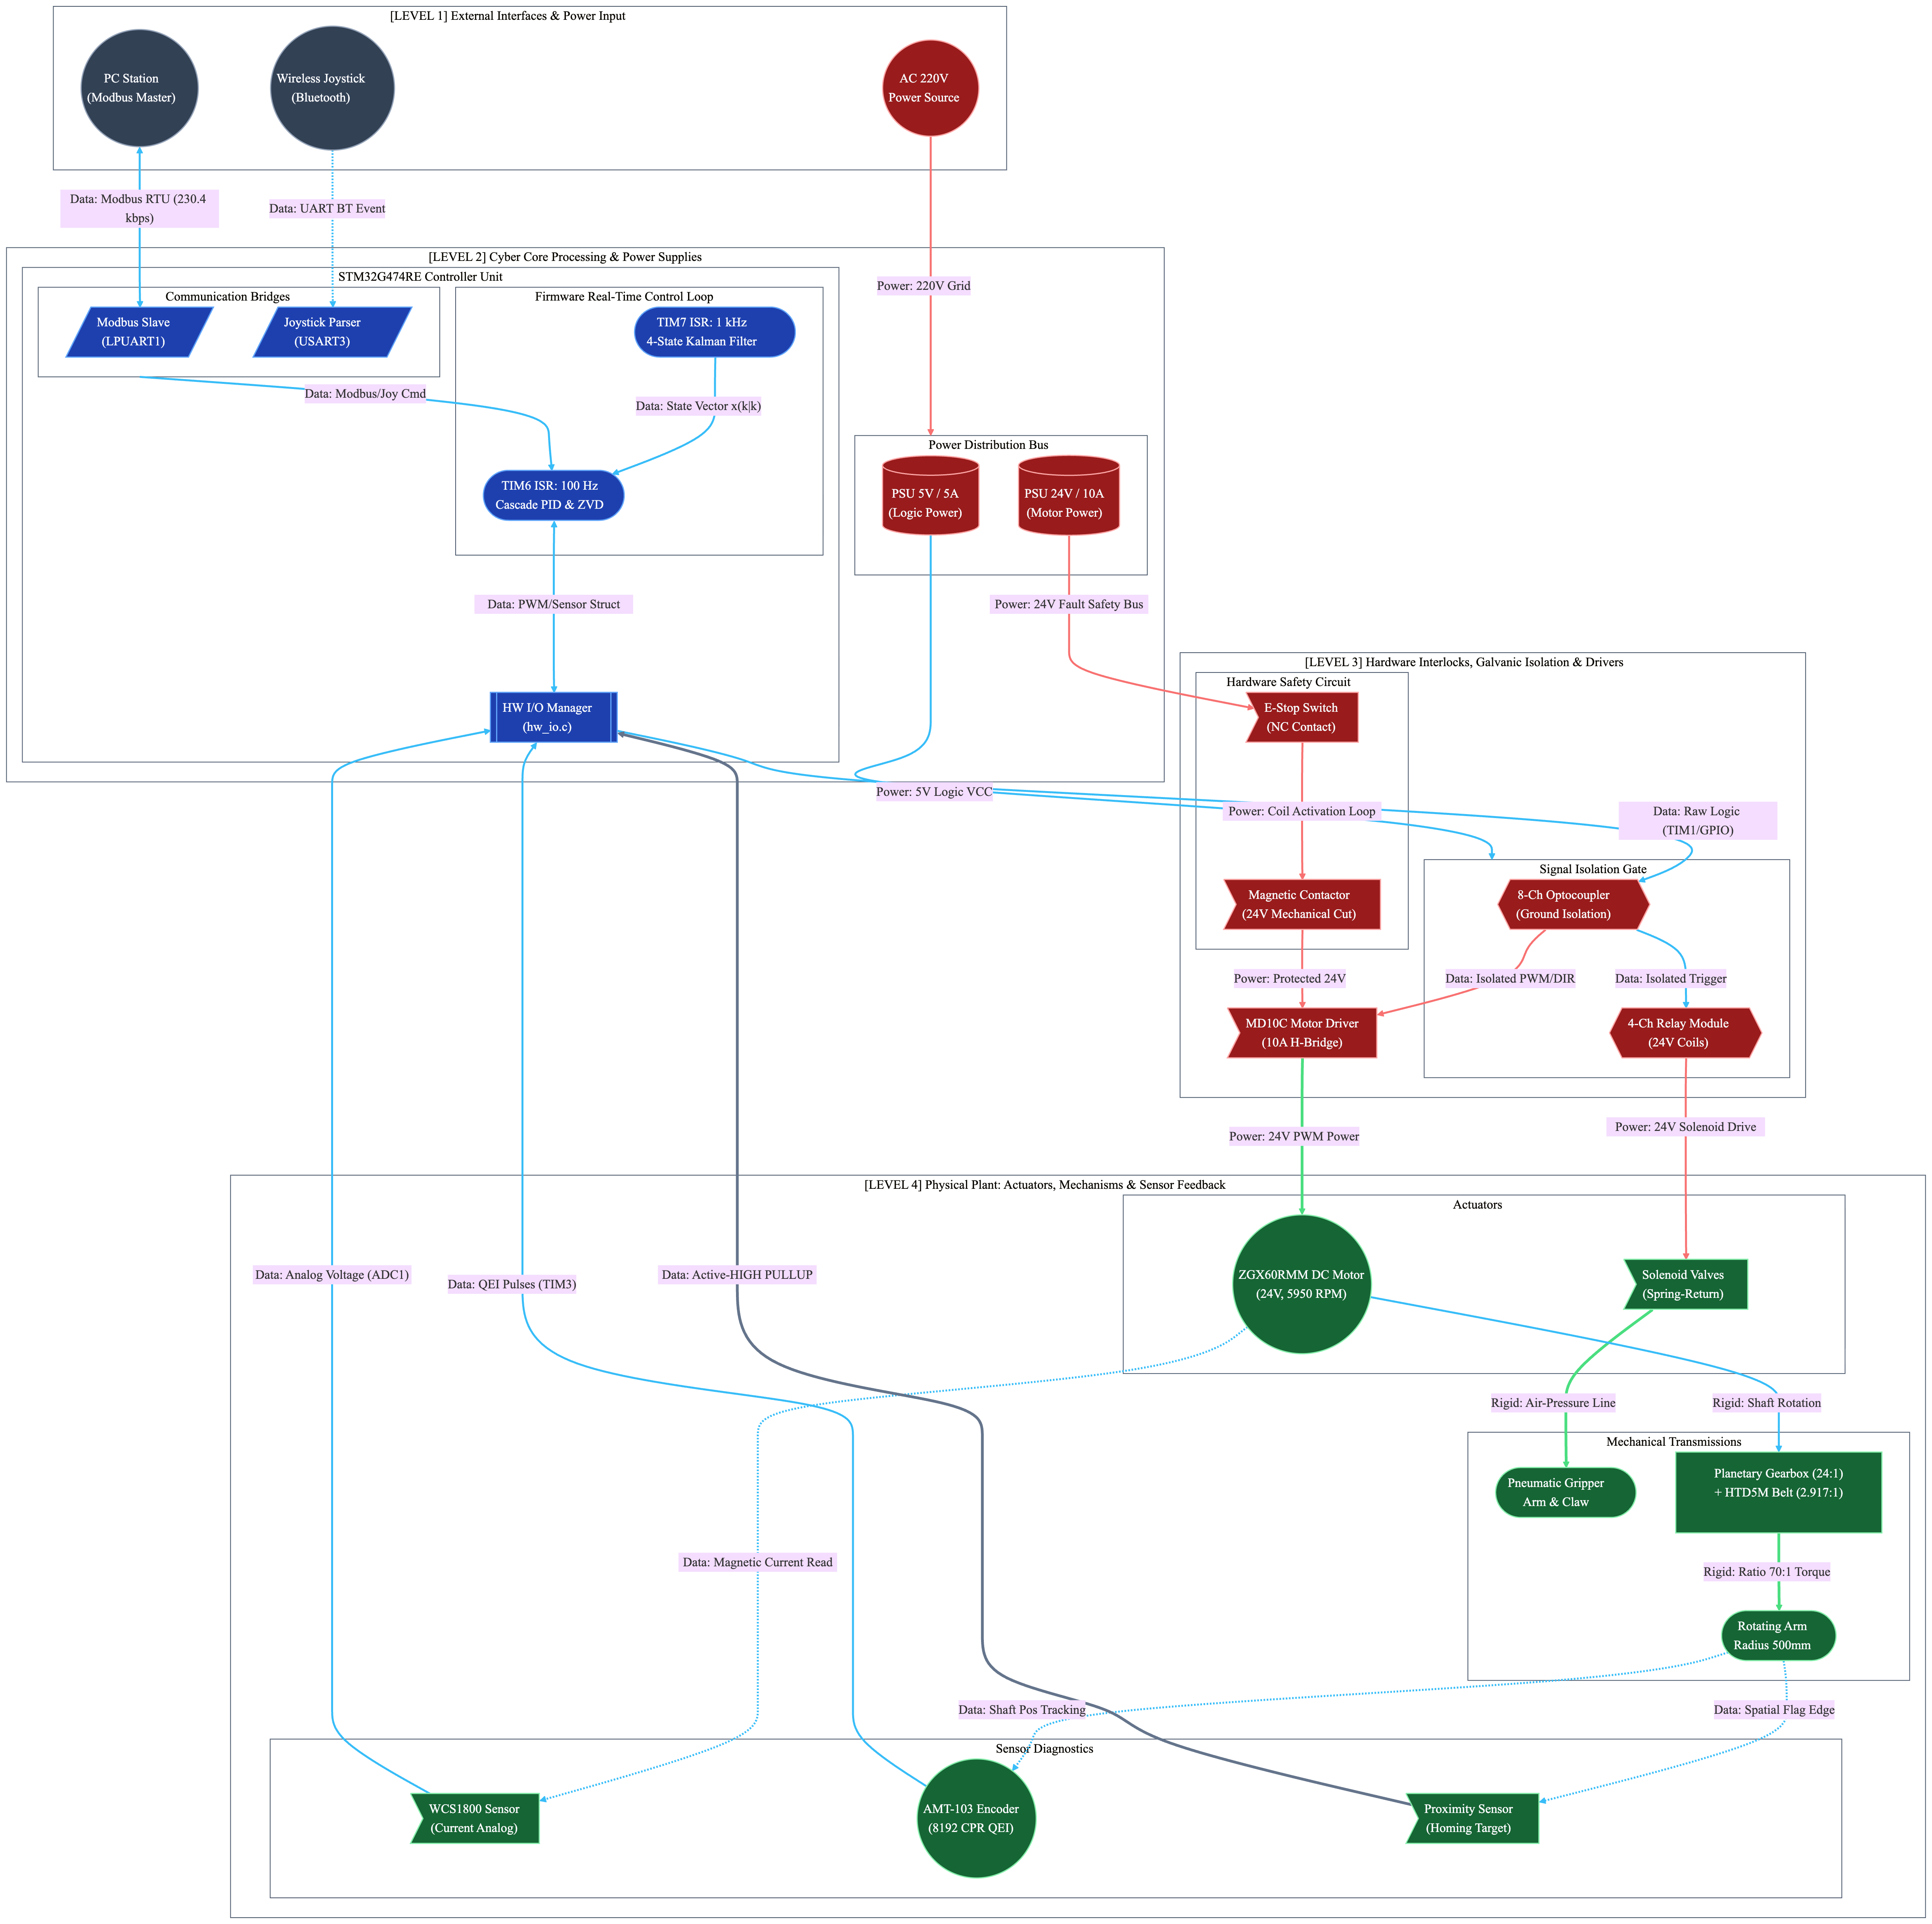
\includegraphics[width=0.95\textwidth]{fig_system_architecture}
    \caption{System Architecture ของระบบ Circular Pick and Place Robot
             แสดง Physical Architecture และ Cyber Architecture}
    \label{fig:sys_arch}
\end{figure}

\begin{itemize}
    \item \textbf{\color[HTML]{38BDF8} เส้นสีฟ้า (Data / Signal Line):} หมายถึง เส้นทางเดินของข้อมูลและสัญญาณควบคุมลอจิกแรงดันต่ำ (Low-voltage Logic) ประกอบด้วยโปรโตคอลการสื่อสารความเร็วสูง เช่น Modbus RTU (230.4 kbps) ผ่าน LPUART1, สัญญาณ Bluetooth จาก Joystick เข้า USART3 รวมถึงสัญญาณพัลส์จาก Quadrature Encoder (TIM3 QEI), สัญญาณอนาล็อกเชิงวินิจฉัยจาก Current Sensor (ADC1 DMA) และสัญญาณทริกเกอร์ลอจิกผ่าน Optocoupler
    
    \item \textbf{\color[HTML]{F87171} เส้นสีแดง (Power \& Safety Interlock Line):} หมายถึง เส้นทางเดินระบบไฟฟ้ากำลังและการกระจายพลังงาน (Power Distribution) รวมถึงวงจรตัดการทำงานฉุกเฉินระดับฮาร์ดแวร์ (Hardware Safety Loop) ได้แก่ สายไฟฟ้ากระแสสลับ 220VAC Grid Input, ระบบบัสแรงดันไฟตรง 24VDC สำหรับขับมอเตอร์และโซลินอยด์วาล์ว, ระบบบัส 5VDC สำหรับเลี้ยงวงจรลอจิก และสายสัญญาณ NC Contact ของ E-Stop ที่เชื่อมต่อไปยัง Magnetic Contactor เพื่อทำ Hardware Interlock
    
    \item \textbf{\color[HTML]{4ADE80} เส้นสีเขียว (Mechanical \& Force Transmission Line):} หมายถึง เส้นทางการส่งถ่ายกำลังเชิงกล แรงบิด และพลังงานไหลเวียน (Kinetic \& Pneumatic Energy Flow) ประกอบด้วยแรงบิดรอบสูงจากเพลามอเตอร์เข้าสู่ Planetary Gearbox (24:1), การส่งกำลังผ่านสายพาน HTD5M Belt Drive (2.917:1) เพื่อขับแขนกลหมุน (Rotating Arm) ด้วยอัตราทดรวม 70:1 รวมถึงแรงดันลม (Pneumatic Pressure) จาก Solenoid Valves ที่ส่งตรงไปขับเคลื่อนกลไกการหยิบจับของตัว Pneumatic Gripper ทั้งในส่วนของกระบอกสูบแนวตั้งและปากจับ
\end{itemize}

ระบบแบ่งออกเป็น 4 Subsystem หลักที่ทำงานร่วมกัน ดังนี้

\paragraph{Rotating Mechanism}
เป็นส่วนที่แปลงพลังงานไฟฟ้าจาก DC Motor ให้กลายเป็นการเคลื่อนที่เชิงมุมของแขนกล
กำลังถูกส่งผ่าน Planetary Gearbox อัตราทด $N_g = 24$
ต่อด้วย Belt Drive HTD5M อัตราทด $N_b = 2.9$
รวมอัตราทดทั้งหมด $N = 70$ ก่อนถึงแขนกลรัศมี 500 mm
ตำแหน่งเชิงมุมวัดโดย Encoder AMT-103 ที่ติดตั้งโดยตรงที่ Output Shaft
เพื่อหลีกเลี่ยง Backlash Error จากระบบส่งกำลัง

\paragraph{Power Management System}
จ่ายพลังงานแก่ทุก Subsystem โดยแบ่งเป็น 2 Bus
High Power Bus (24\,V/10\,A) จ่ายให้มอเตอร์ผ่าน Magnetic Contactor
ที่ถูกควบคุมโดย E-Stop
และ Logic Bus (5\,V) จ่ายให้ STM32, ESP32 และ Sensor
โดยต่อก่อน Contactor ทำให้ Controller ยังมีไฟเลี้ยงแม้กด E-Stop
ตามข้อกำหนด E6

\paragraph{Main Controller}
STM32G474RE ทำหน้าที่เป็นศูนย์กลางประมวลผลทั้งหมด
รัน Cascade PID Control Loop โดยมี Velocity Inner Loop ที่ความถี่ 1\,kHz
และ Position Outer Loop ที่ความถี่ 100\,Hz
พร้อม Kalman Filter 4 สถานะสำหรับประมาณค่าตำแหน่ง ความเร็ว กระแส
และแรงบิดรบกวน
และ ZVD Input Shaper ($f_n = 12.13$\,Hz, $\zeta = 0.041$)
สำหรับลด Residual Vibration ของชิ้นงาน
รับส่งข้อมูลกับ Base System ผ่าน Modbus RTU บน LPUART1
(230400 bps, 8N1, Slave Address~21)

\paragraph{Application FSM}
ระบบมี State Machine หลัก 5 สถานะ ได้แก่
\texttt{INIT} $\rightarrow$ \texttt{HOMING} $\rightarrow$
\texttt{IDLE} $\rightarrow$ \texttt{RUNNING} และ \texttt{FAULT}
โดยทุกสถานะสามารถเข้าสู่ \texttt{FAULT} ได้จาก E-Stop หรือ Safety Fault
และกลับสู่ \texttt{IDLE} ได้เมื่อ Release E-Stop และกด Reset

\paragraph{External Interface}
รองรับการสั่งงาน 2 โหมด ได้แก่
Manual Mode ผ่าน Wireless Joystick ที่รับสัญญาณ Bluetooth ด้วย ESP32
และส่งต่อผ่าน USART3 มายัง STM32
และ Auto Mode ผ่าน Base System ของลูกค้าโดยรับคำสั่งผ่าน Modbus RTU
การควบคุม Gripper ใช้สัญญาณ Digital I/O โดยตรง

\begin{table}[H]
  \centering
  \caption{สรุป Subsystem หลักของระบบ}
  \label{tab:subsystem_summary}
  \begin{tabular}{l p{7.0cm} p{4.5cm}}
    \toprule
    \textbf{Subsystem} & \textbf{องค์ประกอบหลัก} & \textbf{รายละเอียดใน} \\
    \midrule
    Rotating Mechanism
      & \raggedright DC Motor RS-775, Planetary Gearbox ($N_g{=}24$),
        Belt HTD5M ($N_b{=}2.9$), Encoder AMT-103
      & \cref{subsec:mech_arch} \\[0.4em]
    Power Management
      & \raggedright PSU 24\,V/10\,A, PSU 5\,V,
        Magnetic Contactor, E-Stop,
        Circuit Breaker, Fuse
      & \cref{subsec:elec_arch} \\[0.4em]
    Main Controller
      & \raggedright STM32G474RE, Cascade PID (1\,kHz / 100\,Hz),
        Kalman Filter (4 states),
        ZVD Input Shaper,
        Modbus RTU Slave (Addr~21)
      & \cref{subsec:sysid}, \cref{subsec:pid_design} \\[0.4em]
    External Interface
      & \raggedright Joystick + ESP32 (Bluetooth/USART3),
        Base System (Modbus RTU),
        Gripper (Digital I/O)
      & \cref{subsec:joystick_integration}, \cref{subsec:modbus_integration} \\
    \bottomrule
  \end{tabular}
\end{table}

% ----------------------------------------------------------------------------
\section{โครงสร้างของรายงาน}
\label{sec:report_structure}

รายงานฉบับนี้จัดแบ่งเนื้อหาออกเป็น 6 บทหลัก ดังนี้

\begin{enumerate}
  \item \textbf{บทที่ 1 บทนำ:}
        อธิบายที่มาและความสำคัญ วัตถุประสงค์ ขอบเขต
        ข้อกำหนดของระบบทั้ง 32 ข้อ และภาพรวมสถาปัตยกรรมระบบ

  \item \textbf{บทที่ 2 ทฤษฎีและเทคโนโลยีที่เกี่ยวข้อง:}
        นำเสนอทฤษฎีพื้นฐานที่ใช้ในการออกแบบ ได้แก่
        DC Motor State-Space, Cascade PID, ZV Input Shaping,
        Kalman Filter, มาตรฐาน ASME/ISO และ S-Curve Trajectory

  \item \textbf{บทที่ 3 สถาปัตยกรรมและการออกแบบระบบ:}
        นำเสนอรายละเอียดการออกแบบเชิงกล ไฟฟ้า และระบบควบคุม
        รวมถึงการระบุระบบ (System Identification) และการออกแบบตัวควบคุม

  \item \textbf{บทที่ 4 การสร้างและบูรณาการระบบ:}
        บันทึกขั้นตอนการประกอบจริงและการพัฒนา Firmware
        รวมถึงการเชื่อมต่อระบบย่อยทั้งหมดเข้าด้วยกัน

  \item \textbf{บทที่ 5 ผลการทดสอบและการทวนสอบ:}
        รายงานผลการทดสอบเชิงประจักษ์และการทวนสอบข้อกำหนด 32 ข้อ
        พร้อมตาราง Requirements Traceability

  \item \textbf{บทที่ 6 สรุปผลและข้อเสนอแนะ:}
        สรุปภาพรวมความสำเร็จ ปัญหาที่พบ บทเรียนที่ได้
        และแนวทางการพัฒนาต่อยอด
\end{enumerate}
% ============================================================================
%  บทที่ 2: ทฤษฎีและเทคโนโลยีที่เกี่ยวข้อง
% ============================================================================

\chapter{ทฤษฎีและเทคโนโลยีที่เกี่ยวข้อง}
\label{ch:theory}

% ============================================================================
\section{พลศาสตร์ของมอเตอร์กระแสตรง}
\label{sec:dc_motor_model}
% ============================================================================

มอเตอร์กระแสตรง (DC Motor) สามารถจำลองพฤติกรรมได้จากสมการสองโดเมน
ได้แก่ โดเมนวงจรไฟฟ้าและโดเมนพลศาสตร์เชิงกล
โดยทั้งสองโดเมนเชื่อมโยงกันผ่านค่าคงที่ของมอเตอร์
ก่อนการสร้างแบบจำลองทางคณิตศาสตร์ ได้กำหนดสมมติฐานเพื่อลดความซับซ้อนของระบบให้สามารถวิเคราะห์แบบระบบเชิงเส้นไม่แปรผันตามเวลา (Linear Time-Invariant: LTI) ได้ดังนี้

\begin{itemize}
    \item วงจรแม่เหล็กทำงานในช่วงเชิงเส้น (Linear Magnetic Circuit) และไม่เกิดการอิ่มตัวของแกนเหล็ก
    \item ค่าความต้านทาน $R_a$ และตัวเหนี่ยวนำ $L_a$ ของอาร์เมเจอร์มีค่าคงที่ ไม่เปลี่ยนแปลงตามอุณหภูมิที่เพิ่มขึ้น
    \item ละทิ้งผลของแรงดันตกคร่อมที่แปรงถ่าน (Brush Voltage Drop) และแรงเสียดทานสถิต (Coulomb Friction)
\end{itemize}

% ----------------------------------------------------------------------------
\subsection{สมการโดเมนไฟฟ้า}
\label{subsec:electrical_eq}

วงจรอาร์เมเจอร์ประกอบด้วยความต้านทาน $R_a$ และตัวเหนี่ยวนำ $L_a$
ต่อในอนุกรมกับแรงเคลื่อนไฟฟ้าย้อนกลับ (Back-EMF) $e_b$
ตามกฎแรงดันของ Kirchhoff ได้สมการ

% -----------------------------------------------------------------------
% รูปที่ 1: แผนภาพ Electro-mechanical ของ DC Motor
% ชื่อไฟล์แนะนำ: fig_dc_motor_model.pdf
% เนื้อหา: แสดงวงจรไฟฟ้า (Va, Ra, La, eb) เชื่อมต่อกับเพลาทางกล (J, B, tm, td)
% -----------------------------------------------------------------------
\begin{figure}[H]
    \centering
    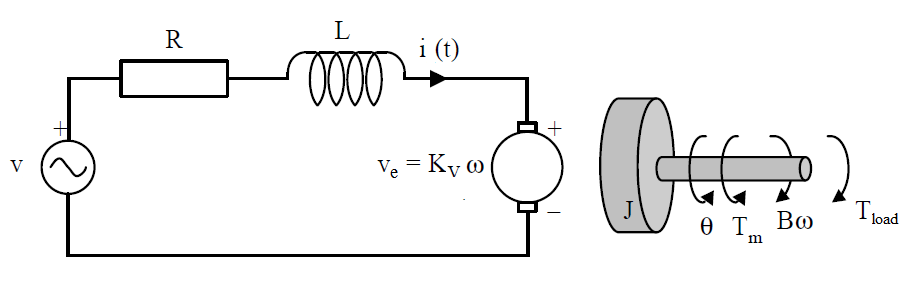
\includegraphics[width=0.8\textwidth]{fig_dc_motor_model}
    \caption{แผนภาพ Electro-mechanical ของมอเตอร์กระแสตรง แสดงความสัมพันธ์ระหว่างโดเมนไฟฟ้าและโดเมนเชิงกล}
    \label{fig:dc_motor_model}
\end{figure}

\begin{equation}
    V_a(t) = R_a\, i_a(t) + L_a\, \frac{di_a(t)}{dt} + e_b(t)
    \label{eq:armature_voltage}
\end{equation}

\noindent โดยที่ $e_b = K_b\,\omega_m$ และ $K_b$ คือค่าคงที่ Back-EMF (\si{\volt\second\per\radian})
กำหนดให้ $\omega_m$ คือความเร็วเชิงมุมที่เพลามอเตอร์ ซึ่งมีความสัมพันธ์กับความเร็วเชิงมุมที่เพลา Output $\omega$ (หลัง Gearbox อัตราทด $N$) ตามความสัมพันธ์ทางจลนศาสตร์ $\omega_m = N\omega$
ดังนั้นเมื่อแทนค่ากลับลงใน\cref{eq:armature_voltage} จะได้สมการเชิงอนุพันธ์ของโดเมนไฟฟ้าที่สอดคล้องกับความเร็วเพลา Output ดังนี้

\begin{equation}
    L_a\, \frac{di_a}{dt} = V_a - R_a\, i_a - K_b\,N\,\omega
    \label{eq:electrical_ode}
\end{equation}

% ----------------------------------------------------------------------------
\subsection{สมการโดเมนเชิงกล}
\label{subsec:mechanical_eq}

แรงบิดแม่เหล็กไฟฟ้า $\tau_m$ ที่มอเตอร์ผลิตได้เป็นสัดส่วนกับกระแสอาร์เมเจอร์ $i_a$

\begin{equation}
    \tau_m = K_t\, i_a
    \label{eq:motor_torque}
\end{equation}

\noindent โดยที่ $K_t$ คือค่าคงที่แรงบิด (\si{\newton\metre\per\ampere})
ทั้งนี้ ตามหลักการอนุรักษ์พลังงานในอุดมคติของระบบหน่วย SI กำลังงานเชิงกลที่สร้างได้จะเท่ากับกำลังงานไฟฟ้าที่ป้อนเข้า (Mechanical Power = Electrical Power) ส่งผลให้ค่าคงที่แรงบิดและค่าคงที่ Back-EMF มีค่าเท่ากันในเชิงตัวเลข ($K_t = K_b$)

กฎที่สองของนิวตันสำหรับการหมุนที่ประยุกต์ใช้กับเพลา Output (พิจารณาผ่าน Gearbox อัตราทด $N$ และประสิทธิภาพ $\eta$) จะได้

\begin{equation}
    J\, \frac{d\omega}{dt} = \eta\, N\, K_t\, i_a - B\,\omega - \tau_d
    \label{eq:mechanical_ode}
\end{equation}

\noindent โดยที่ $J$ คือโมเมนต์ความเฉื่อยรวมทั้งหมดที่ Reflect กลับมายังเพลา Output (\si{\kilogram\metre\squared}),
$B$ คือค่าสัมประสิทธิ์แรงหน่วงหนืด (\si{\newton\metre\second\per\radian}),
และ $\tau_d$ คือแรงบิดรบกวนจากภายนอก

% ----------------------------------------------------------------------------
\subsection{State-Space Representation}
\label{subsec:state_space}

นิยาม State Vector $\mathbf{x} = [\theta,\; \omega,\; i_a,\; \tau_d]^\top$
โดยที่ $\theta$ คือมุมตำแหน่ง (rad), $\omega$ คือความเร็วเชิงมุม (rad/s),
$i_a$ คือกระแสอาร์เมเจอร์ (A) และ $\tau_d$ คือแรงบิดรบกวนที่ Augment เพิ่มเข้ามา
ระบบ 4 สถานะในรูปแบบ Continuous-Time State-Space เขียนได้เป็น

\begin{equation}
    \dot{\mathbf{x}} = \mathbf{A}\mathbf{x} + \mathbf{B}u, \qquad
    y = \mathbf{C}\mathbf{x}
    \label{eq:state_space_ct}
\end{equation}

\noindent โดยที่

\begin{equation}
    \mathbf{A} = \begin{bmatrix}
        0 & 1 & 0 & 0 \\
        0 & -\tfrac{B}{J} & \tfrac{\eta N K_t}{J} & -\tfrac{1}{J} \\
        0 & -\tfrac{K_b N}{L_a} & -\tfrac{R_a}{L_a} & 0 \\
        0 & 0 & 0 & 0
    \end{bmatrix}, \quad
    \mathbf{B} = \begin{bmatrix} 0 \\ 0 \\ \tfrac{1}{L_a} \\ 0 \end{bmatrix}, \quad
    \mathbf{C} = \begin{bmatrix} 1 & 0 & 0 & 0 \end{bmatrix}
    \label{eq:ABCD_matrices}
\end{equation}

\noindent input $u = V_a$ คือแรงดันที่จ่ายให้อาร์เมเจอร์ และ output $y = \theta$ 
(เนื่องจากเซนเซอร์สามารถวัดได้เพียงตำแหน่งเชิงมุม)
สถานะ $\tau_d$ เป็น Augmented State ที่ถือว่าเปลี่ยนแปลงช้า ($\dot{\tau}_d \approx 0$)
ใช้สำหรับเป็น State Estimator ใน Kalman Filter เพื่อประมาณค่าความเร็วและแรงบิดรบกวนแบบ Real-time
ตามที่อธิบายใน\cref{subsec:kalman_filter}

% ============================================================================
\section{ทฤษฎีการควบคุมและการกรองสัญญาณ}
\label{sec:control_theory}
% ============================================================================

% ----------------------------------------------------------------------------
\subsection{Cascade PID Control}
\label{subsec:cascade_pid}

โครงสร้าง Cascade PID ประกอบด้วยวงรอบควบคุมสองชั้นที่ซ้อนกัน
โดยวงรอบใน (Inner Loop) ควบคุมความเร็วเชิงมุม $\omega$
และวงรอบนอก (Outer Loop) ควบคุมตำแหน่งเชิงมุม $\theta$

% -----------------------------------------------------------------------
% รูปที่ 2: Block Diagram ของ Cascade PID
% ชื่อไฟล์แนะนำ: fig_cascade_pid_block.pdf
% เนื้อหา: Block diagram แสดง Position Outer Loop และ Velocity Inner Loop
%          พร้อม ZVD Shaper ที่ input และ Anti-windup ในวง velocity
% -----------------------------------------------------------------------
\begin{figure}[H]
    \centering
    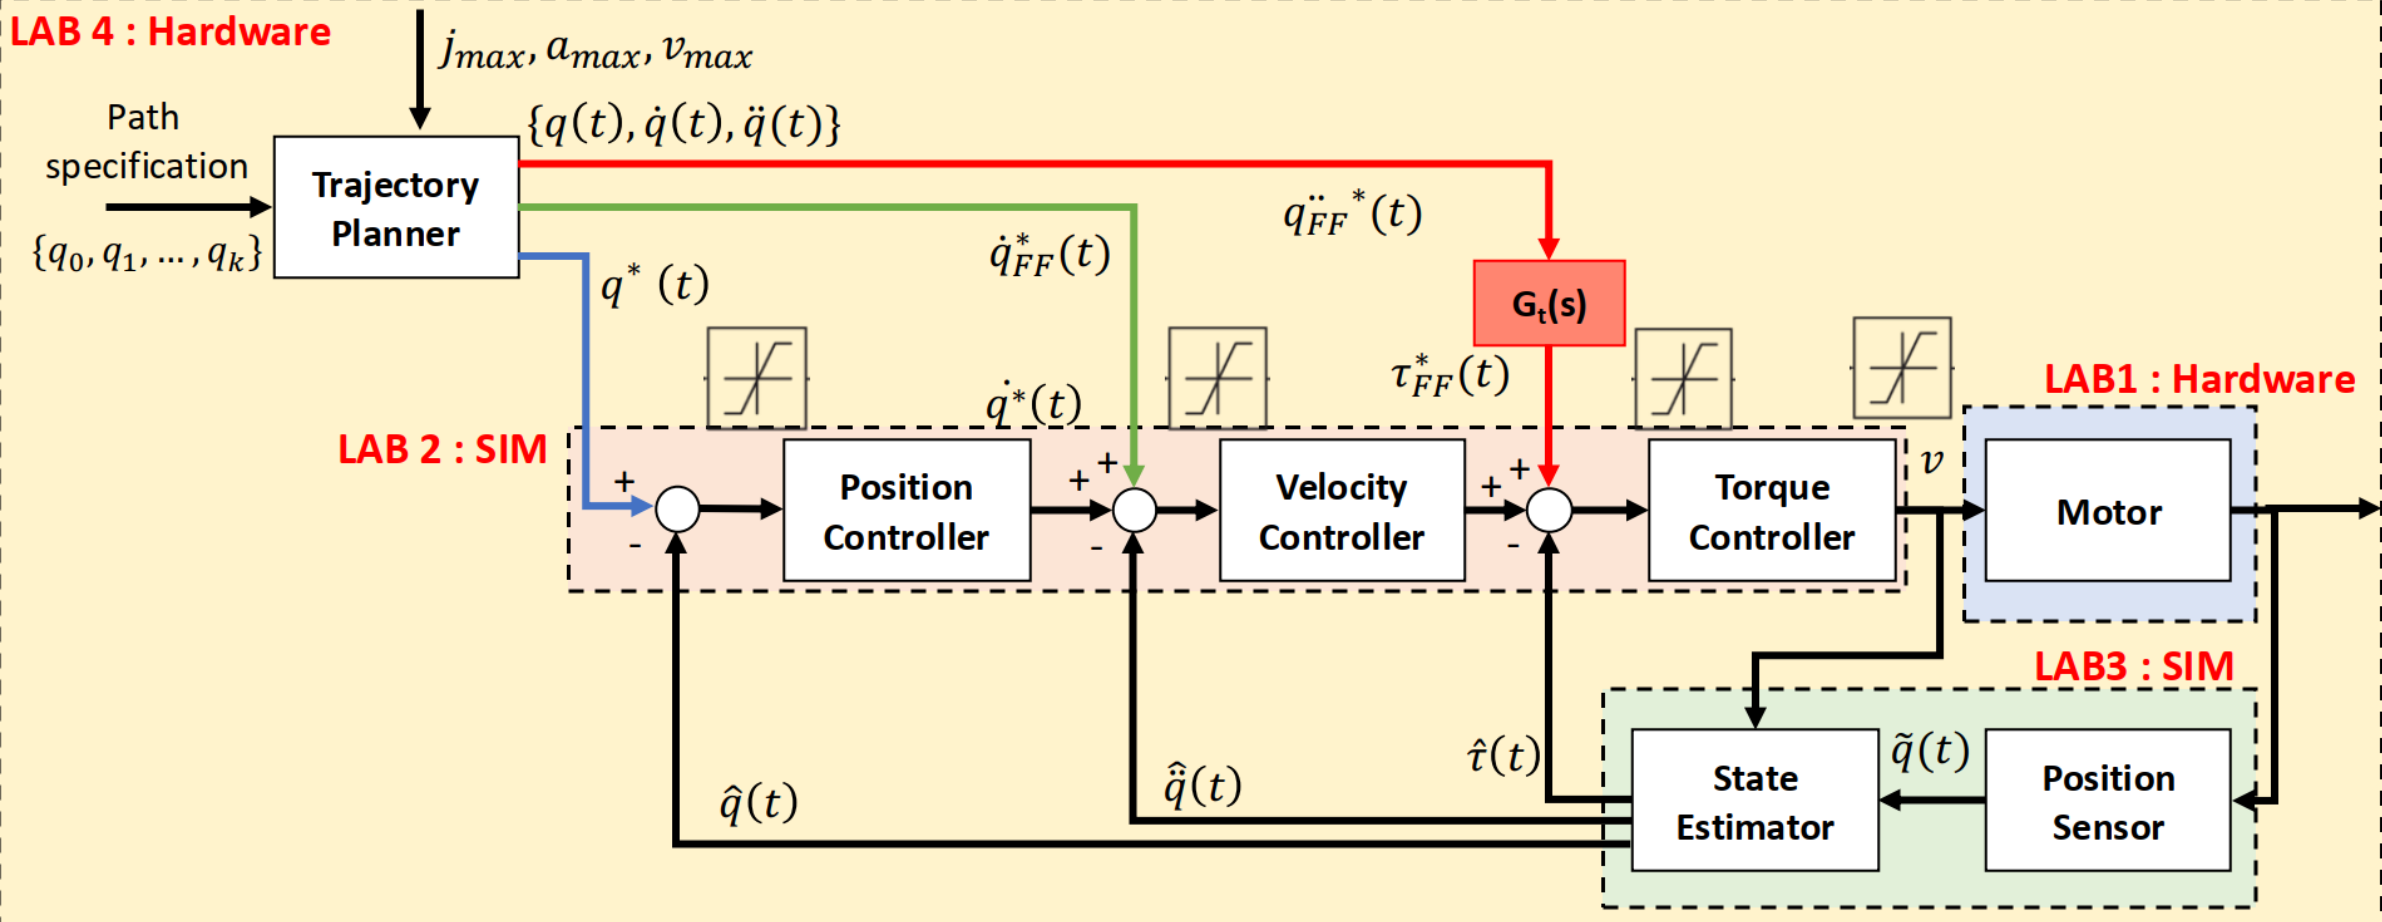
\includegraphics[width=1.0\textwidth]{fig_cascade_pid_block}
    \caption{Block Diagram ของระบบควบคุม Cascade PID
             แสดงวงรอบความเร็วและวงรอบตำแหน่ง}
    \label{fig:cascade_pid_block}
\end{figure}

\subsubsection{Velocity Inner Loop}

ตัวควบคุม PID สำหรับวงรอบความเร็วมี Transfer Function ในรูป

\begin{equation}
    C_v(s) = K_{p,v} + \frac{K_{i,v}}{s} + K_{d,v}\,s
    \label{eq:pid_velocity}
\end{equation}

\noindent ความถี่ Sampling ของวงรอบความเร็วกำหนดที่ $f_v = 1$\,kHz ($T_v = 1$\,ms)
การ Discretize ตัวควบคุมเข้าสู่ Digital Domain ใช้วิธี Tustin (Bilinear Transformation) 
สาเหตุที่เลือกใช้วิธีนี้แทนวิธี Forward Euler เพื่อป้องกันปัญหาความไม่เสถียร เนื่องจากวิธี Tustin 
จะทำการ Map โพล (Pole) ฝั่งซ้ายของระนาบ $s$ ให้อยู่ภายใน Unit Circle ของระนาบ $z$ อย่างสมบูรณ์ 
(Preserve Stability) โดยเฉพาะเมื่อระบบมีอัตราส่วน $K_{i,v} / f_v$ ที่มีขนาดใหญ่

\begin{equation}
    s \;\longrightarrow\; \frac{2}{T_v}\cdot\frac{z-1}{z+1}
    \label{eq:tustin}
\end{equation}

ค่า Gain ที่ใช้ในระบบจริงได้จาก Hardware Commissioning
และแสดงรายละเอียดไว้ใน\cref{subsec:pid_design} และ\cref{tab:pid_gains}
นอกจากนี้ยังมีการเพิ่มระบบ Anti-windup แบบ Back-Calculation เพื่อป้องกันปัญหา Integral Windup 
เมื่อแรงดัน Output อิ่มตัวที่ $\pm$24\,V โดยค่า Integrator State ($I_k$) จะถูกอัปเดตในแต่ละ Time Step ตามสมการ

\begin{equation}
    I_k = I_{k-1} + K_{i,v}\, T_v\, e_k + K_{bc} \left(u_{sat,k} - u_{unsat,k}\right)
    \label{eq:anti_windup}
\end{equation}

\noindent โดยที่ $K_{bc}$ คือ Anti-windup Tracking Gain, $u_{sat,k}$ คือแรงดันควบคุมที่ถูกจำกัดแล้ว 
และ $u_{unsat,k}$ คือแรงดันควบคุมที่คำนวณได้ก่อนเข้า Saturation Block

\subsubsection{Position Outer Loop}

ตัวควบคุม PID สำหรับวงรอบตำแหน่งมีโครงสร้างเดียวกับ\cref{eq:pid_velocity}
โดย Output ของ Outer Loop คือ Velocity Setpoint ที่ส่งเข้าสู่ Inner Loop
ความถี่ Sampling กำหนดที่ $f_p = 100$\,Hz ($T_p = 10$\,ms)

\subsubsection{หลักการออกแบบ Cascade}

การออกแบบวงรอบทั้งสองต้องปฏิบัติตามกฎ Bandwidth Separation
โดย Bandwidth ของ Inner Loop ต้องสูงกว่า Outer Loop อย่างน้อย 5 เท่า
เพื่อให้ Inner Loop ตอบสนองเร็วพอที่จะถูกมองเป็น Unity Gain จาก Outer Loop
การออกแบบในโครงงานนี้ใช้ Root Locus โดยออกแบบ Inner Loop ก่อน
แล้วจึงใช้ Transfer Function ของ Closed-Loop Inner Loop
เป็น Plant ที่แท้จริงสำหรับการออกแบบ Outer Loop

% ----------------------------------------------------------------------------
\subsection{ZVD Input Shaping}
\label{subsec:zv_shaping}

Input Shaping เป็นเทคนิคการปรับ Command Signal ก่อนส่งเข้าระบบ
โดยการ Convolve คำสั่งเดิมกับ Impulse Sequence ที่ออกแบบมาเพื่อยกเลิก
การแกว่งของระบบที่ความถี่ธรรมชาติ $\omega_n$

% -----------------------------------------------------------------------
% รูปที่ 3: กราฟการทำงานของ ZVD Shaper
% ชื่อไฟล์แนะนำ: fig_zvd_response.pdf
% เนื้อหา: กราฟ 2 รูปย่อย (บน: Impulse Sequence 3 ค่า, ล่าง: การตอบสนองของระบบก่อนและหลังทำ Shaping)
% -----------------------------------------------------------------------
\begin{figure}[H]
    \centering
    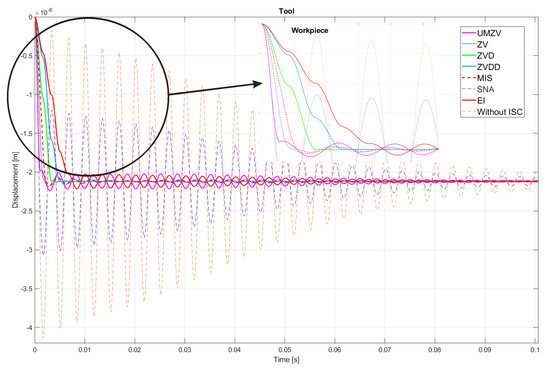
\includegraphics[width=0.9\textwidth]{fig_zvd_response}
    \caption{ลักษณะของสัญญาณ ZVD Impulse Sequence (บน) และเปรียบเทียบการตอบสนองของระบบเพื่อลดการแกว่ง (ล่าง)}
    \label{fig:zvd_response}
\end{figure}

\subsubsection{โครงสร้างของ ZVD Shaper}

ZVD Shaper ใช้ Impulse สามอัน $(A_1, t_1)$, $(A_2, t_2)$, $(A_3, t_3)$
โดยกำหนด $t_1 = 0$ และ Delay ที่เหลือคำนวณจากคาบ Damped Oscillation

\begin{equation}
    t_2 = T_d = \frac{\pi}{\omega_n\sqrt{1-\zeta^2}}, \qquad t_3 = 2T_d
    \label{eq:zv_t2}
\end{equation}

\noindent แอมพลิจูดของ Impulse คำนวณจากเงื่อนไข Zero Residual Vibration,
Zero Derivative ของ Residual Vibration และผลรวมขนาดยอดเท่ากับ 1

\begin{equation}
    K = e^{-\zeta\pi/\sqrt{1-\zeta^2}}, \qquad
    A_1 = \frac{1}{(1+K)^2}, \quad
    A_2 = \frac{2K}{(1+K)^2}, \quad
    A_3 = \frac{K^2}{(1+K)^2}
    \label{eq:zv_amplitudes}
\end{equation}

\noindent ZVD มีความทนทานต่อความคลาดเคลื่อนของ $\omega_n$ สูงกว่า ZV (2-Impulse)
โดยแลกกับ Delay เพิ่มขึ้น $T_d$
ค่า $\omega_n$ และ $\zeta$ ของ Connection Rod วัดจาก Hardware
และพารามิเตอร์ ZVD ที่ได้แสดงใน\cref{tab:zvd_params}

\subsubsection{การ Implementation บน Embedded System (Discrete-Time)}

สำหรับการทำงานจริงบนไมโครคอนโทรลเลอร์ (STM32G474RE) ระบบทำงานในรูปแบบ Discrete-time ตามความถี่ของ Position Loop ($T_p = 10$\,ms) 
ดังนั้นเวลาหน่วง $t_2$ และ $t_3$ ที่คำนวณได้ จะต้องถูกปัดเศษให้เป็นจำนวนเต็มของ Sample ($N_d$) เพื่อใช้งานใน Circular Buffer

\begin{equation}
    N_2 = \text{round}\left(\frac{t_2}{T_p}\right), \qquad N_3 = \text{round}\left(\frac{t_3}{T_p}\right)
    \label{eq:zvd_discrete_delay}
\end{equation}

\noindent ส่งผลให้ Transfer Function ของ ZVD Shaper ในโดเมน $z$ สามารถเขียนได้เป็น

\begin{equation}
    F(z) = A_1 + A_2\, z^{-N_2} + A_3\, z^{-N_3}
    \label{eq:zvd_transfer_function}
\end{equation}

\noindent โดย Command Signal $r(t)$ จะถูกประมวลผลผ่านสมการ\cref{eq:zvd_transfer_function} 
ซึ่งให้ผลเทียบเท่าการ Convolve ใน Discrete-time ก่อนส่งเข้า Position Outer Loop

\subsubsection{ความสำคัญต่อ Cycle Time}

หากไม่ใช้ Input Shaper ชิ้นงาน Connection Rod จะแกว่งหลังจากแขนกลหยุด
โดย Settling Time ของการแกว่งดังกล่าวอยู่ที่ประมาณ 6--7 วินาทีต่อการเคลื่อนที่หนึ่งครั้ง
ซึ่งทำให้ Cycle Time ทั้งหมดเกิน 35 วินาทีอย่างแน่นอน
ZVD Shaper แก้ปัญหานี้โดยเพิ่มเวลาหน่วงรวมเพียง $t_3 \approx 80$\,ms ต่อการเคลื่อนที่
% ----------------------------------------------------------------------------
% ----------------------------------------------------------------------------
\subsection{Kalman Filter}
\label{subsec:kalman_filter}

Kalman Filter เป็นตัวประมาณค่าสถานะ (State Estimator) ที่หาค่าเหมาะสมที่สุด (Optimal) ภายใต้สมมติฐานว่า สัญญาณรบกวนกระบวนการ (Process Noise) และสัญญาณรบกวนการวัด (Measurement Noise) มีการกระจายตัวแบบ Gaussian White Noise โดยมี Computational Complexity เป็น $\mathcal{O}(n^2)$ ต่อ Time Step

% -----------------------------------------------------------------------
% รูปที่ 4: Flowchart การทำงานของ Kalman Filter
% ชื่อไฟล์แนะนำ: fig_kalman_flowchart.pdf
% เนื้อหา: Flowchart แบบลูปปิด แสดงขั้นตอน Predict (Time Update) และ Update (Measurement Update)
% -----------------------------------------------------------------------
\begin{figure}[H]
    \centering
    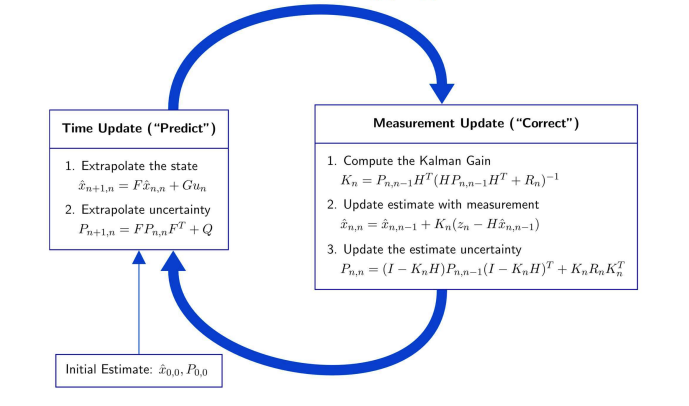
\includegraphics[width=0.85\textwidth]{fig_kalman_flowchart}
    \caption{ขั้นตอนการทำงานของ Discrete-Time Kalman Filter ในแต่ละ Time Step}
    \label{fig:kalman_flowchart}
\end{figure}

\subsubsection{Discrete-Time State-Space Model และ Random Walk}

หนึ่งในความท้าทายหลักของการควบคุมมอเตอร์คือ เซนเซอร์มักจะวัดได้เพียงตำแหน่งเชิงมุม ($\theta$) การหาความเร็วเชิงมุมด้วยการหาอนุพันธ์โดยประมาณ (Approximate Derivative, $\Delta\theta/\Delta t$) จะทำให้เกิด Noise Amplification อย่างรุนแรง นอกจากนี้ ระบบยังเผชิญกับแรงบิดรบกวน ($\tau_d$) ที่ไม่ทราบค่า 

เพื่อแก้ปัญหานี้ แรงบิดรบกวนจึงถูกนำมาต่อขยายในตัวแปรสถานะ (Augmented State) โดยใช้สมมติฐานว่าการเปลี่ยนแปลงของ $\tau_d$ เกิดจากสัญญาณรบกวนแบบสุ่ม (Random Walk) หรือ $\dot{\tau}_d = w_\tau$ 
สำหรับการนำไปใช้งานบน Embedded System ระบบ Continuous-Time ใน\cref{eq:state_space_ct} จะถูกแปลงเป็นเวลาไม่ต่อเนื่อง (Discretization) ด้วยวิธี Zero-Order Hold (ZOH) ที่ Sample Time $T_s$

\begin{equation}
    \mathbf{x}_{k+1} = \mathbf{A}_d\,\mathbf{x}_k + \mathbf{B}_d\,u_k + \mathbf{w}_k, \qquad
    y_k = \mathbf{C}\,\mathbf{x}_k + v_k
    \label{eq:state_space_dt}
\end{equation}

\noindent โดยที่ $\mathbf{w}_k \sim \mathcal{N}(\mathbf{0}, \mathbf{Q})$ คือ Process Noise ของแต่ละสถานะ และ $v_k \sim \mathcal{N}(0, R)$ คือ Measurement Noise

\subsubsection{การกำหนดพารามิเตอร์ Noise ($Q$ และ $R$)}

การกำหนดเมทริกซ์ความแปรปรวนเกี่ยวพัน (Covariance Matrices) มีผลโดยตรงต่อความแม่นยำของตัวกรอง:
\begin{itemize}
    \item \textbf{Measurement Noise ($R$):} สามารถประเมินได้จากความละเอียด (Resolution) ของเซนเซอร์ เช่น หากใช้อุปกรณ์เข้ารหัสสัมบูรณ์ (Absolute Encoder) ขนาด 12-bit จะมีตำแหน่งแยกย่อย 4096 ค่าต่อรอบ (ความละเอียด $\Delta \approx 0.088\degree$) ความแปรปรวนของ Quantization Noise นี้สามารถจำลองด้วย Uniform Distribution ซึ่งมีค่าความแปรปรวน $R = \Delta^2 / 12$
    \item \textbf{Process Noise ($\mathbf{Q}$):} เป็นเมทริกซ์ที่ปรับจูนเพื่อสร้างสมดุลระหว่างความเชื่อมั่นในแบบจำลองทางคณิตศาสตร์กับความเชื่อมั่นในเซนเซอร์ โดยสมาชิกที่ตรงกับสถานะ $\tau_d$ จะเป็นตัวกำหนดความไว (Bandwidth) ในการประมาณค่าแรงบิดรบกวน
\end{itemize}

\subsubsection{Kalman Filter Equations}

กระบวนการทำงานของ Kalman Filter แบ่งเป็นสองขั้นตอนย่อยที่ทำสลับกันทุก Time Step ได้แก่

\noindent\textbf{1. Predict (Time Update):} เป็นการทำนายสถานะล่วงหน้าจากแบบจำลองทางคณิตศาสตร์
\begin{equation}
    \hat{\mathbf{x}}_{k|k-1} = \mathbf{A}_d\,\hat{\mathbf{x}}_{k-1|k-1} + \mathbf{B}_d\,u_{k-1}
    \label{eq:kf_predict_x}
\end{equation}
\begin{equation}
    \mathbf{P}_{k|k-1} = \mathbf{A}_d\,\mathbf{P}_{k-1|k-1}\,\mathbf{A}_d^\top + \mathbf{Q}
    \label{eq:kf_predict_P}
\end{equation}

\noindent\textbf{2. Update (Measurement Update):} เป็นการแก้ไขค่าที่ทำนายด้วยข้อมูลที่วัดได้จริงจากเซนเซอร์
\begin{equation}
    \mathbf{K}_k = \mathbf{P}_{k|k-1}\,\mathbf{C}^\top
                   \left(\mathbf{C}\,\mathbf{P}_{k|k-1}\,\mathbf{C}^\top + R\right)^{-1}
    \label{eq:kf_gain}
\end{equation}
\begin{equation}
    \hat{\mathbf{x}}_{k|k} = \hat{\mathbf{x}}_{k|k-1} + \mathbf{K}_k
                              \left(y_k - \mathbf{C}\,\hat{\mathbf{x}}_{k|k-1}\right)
    \label{eq:kf_update_x}
\end{equation}
\begin{equation}
    \mathbf{P}_{k|k} = \left(\mathbf{I} - \mathbf{K}_k\,\mathbf{C}\right)\mathbf{P}_{k|k-1}
    \label{eq:kf_update_P}
\end{equation}

% -----------------------------------------------------------------------
% รูปที่ 5: กราฟเปรียบเทียบการประมาณค่าความเร็วของ Kalman Filter กับการหาอนุพันธ์
% ชื่อไฟล์แนะนำ: fig_kf_rmse_velocity.pdf
% เนื้อหา: กราฟแสดงความเร็วที่ได้จาก KF ที่เรียบเนียน เทียบกับความเร็วจากการหาอนุพันธ์ที่มี Noise (หรือกราฟ RMSE)
% -----------------------------------------------------------------------
\begin{figure}[H]
    \centering
    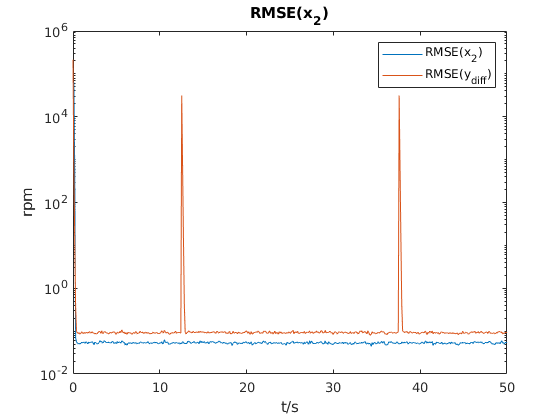
\includegraphics[width=0.9\textwidth]{fig_kf_rmse_velocity}
    \caption{การเปรียบเทียบประสิทธิภาพการประมาณค่าความเร็วเชิงมุมระหว่าง Kalman Filter กับการหาอนุพันธ์โดยประมาณ (Approximate Derivative)}
    \label{fig:kf_rmse_velocity}
\end{figure}

\subsubsection{Steady-State Kalman Gain}

เนื่องจากระบบเชิงเส้นและ Time-Invariant Covariance Matrix $\mathbf{P}$
จะ Converge ไปยังค่า Steady-State $\mathbf{P}_\infty$
ซึ่งสามารถคำนวณล่วงหน้าได้จาก Discrete Algebraic Riccati Equation (DARE)

\begin{equation}
    \mathbf{P}_\infty = \mathbf{A}_d\,\mathbf{P}_\infty\,\mathbf{A}_d^\top - 
    \mathbf{A}_d\,\mathbf{P}_\infty\,\mathbf{C}^\top
    \left(\mathbf{C}\,\mathbf{P}_\infty\,\mathbf{C}^\top + R\right)^{-1}
    \mathbf{C}\,\mathbf{P}_\infty\,\mathbf{A}_d^\top + \mathbf{Q}
    \label{eq:dare}
\end{equation}

\noindent Steady-State Kalman Gain $\mathbf{K}_\infty$ คำนวณครั้งเดียวบน MATLAB
แล้ว Hardcode ลงใน Firmware ทำให้ลด Computational Load บนหน่วยประมวลผลได้อย่างมาก โดยยังคงประสิทธิภาพการประเมินสถานะในระดับที่ใกล้เคียงกับ Optimal Gain

% ============================================================================
\section{มาตรฐานการออกแบบเชิงกล}
\label{sec:mech_standards}
% ============================================================================

% ----------------------------------------------------------------------------
\subsection{การออกแบบเพลา (ASME Shaft Design)}
\label{subsec:shaft_design}

การออกแบบเพลาในโครงงานนี้อ้างอิงมาตรฐาน ASME โดยใช้ทฤษฎีพลังงานความผิดเพี้ยน (Distortion Energy Theory หรือ Von Mises Criterion) สำหรับกรณีที่เพลาต้องรับภาระทั้งโมเมนต์ดัด (Bending Moment) และแรงบิด (Torque) ไปพร้อมกัน 

% -----------------------------------------------------------------------
% รูปที่ 6: Free Body Diagram ของเพลา
% ชื่อไฟล์แนะนำ: fig_shaft_fbd.pdf
% เนื้อหา: FBD แสดงจุดรองรับ (Bearings) และจุดที่เกิดแรงกระทำ เพื่อหา Bending Moment และ Torque
% -----------------------------------------------------------------------
% \begin{figure}[H]
%     \centering
%     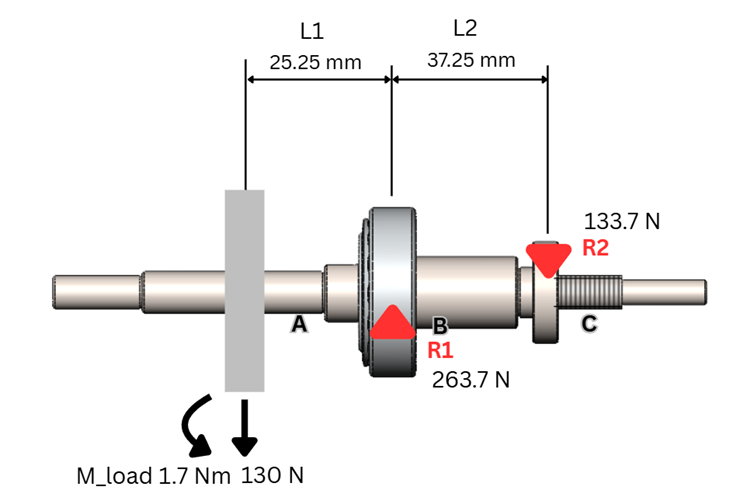
\includegraphics[width=1.0\textwidth]{fig_shaft_fbd}
%     \caption{Free Body Diagram (FBD) ของเพลาแสดงจุดรองรับและภาระที่กระทำในสภาวะการทำงาน}
%     \label{fig:shaft_fbd}
% \end{figure}

\subsubsection{การวิเคราะห์ความล้า (Fatigue Analysis)}

ในการทำงานของระบบขับเคลื่อน เพลาจะรับภาระแบบเปลี่ยนแปลงตามเวลา (Fluctuating Loads) ขนาดเส้นผ่านศูนย์กลางเพลาขั้นต่ำสำหรับการป้องกันความเสียหายจากความล้าคำนวณได้จากสมการ

\begin{equation}
    d \geq \left[\frac{16}{\pi}\cdot\frac{N_s}{S_e}
    \sqrt{\left(K_f M_a\right)^2 + \frac{3}{4}\left(K_{fs} T_a\right)^2}
    \;\right]^{1/3}
    \label{eq:shaft_diameter_fatigue}
\end{equation}

\noindent โดยที่ $N_s$ คือค่าความปลอดภัย (Safety Factor), $K_f$ และ $K_{fs}$ คือตัวคูณความเค้นหนาแน่นสำหรับความล้า (Fatigue Stress Concentration Factor) ของโมเมนต์ดัดและแรงบิดตามลำดับ, $M_a$ คือแอมพลิจูดของโมเมนต์ดัด (\si{\newton\metre}) และ $T_a$ คือแอมพลิจูดของแรงบิด (\si{\newton\metre})

ค่า $S_e$ คือขีดจำกัดความทนทาน (Modified Endurance Limit) (\si{\pascal}) ซึ่งได้จากการปรับลดทอนค่าขีดจำกัดความทนทานในอุดมคติ ($S_e'$) ด้วยปัจจัยอิทธิพลต่างๆ ตามสมการของ Marin (Marin Equation) ดังนี้

\begin{equation}
    S_e = k_a\, k_b\, k_c\, k_d\, k_e\, S_e'
    \label{eq:marin_factors}
\end{equation}

\noindent โดยที่ตัวแปร $k$ ต่างๆ คือปัจจัยปรับแก้ด้านสภาพผิว (Surface), ขนาด (Size), ภาระ (Load), อุณหภูมิ (Temperature) และความน่าเชื่อถือ (Reliability) ตามลำดับ

\subsubsection{การตรวจสอบการครากสถิต (Static Yielding Check)}

นอกจากการวิเคราะห์ความล้าแล้ว เพลาในระบบหุ่นยนต์ที่ต้องทนต่อแรงกระชาก (Jerk) หรือแรงบิดสูงสุดชั่วขณะ (Peak Torque) จากมอเตอร์ จำเป็นต้องได้รับการตรวจสอบไม่ให้เกิดการคราก (Yielding) ในรอบแรกของการทำงาน โดยความเค้นเทียบเท่า (Von Mises Equivalent Stress) สูงสุดจะต้องไม่เกินจุดคราก ($S_y$)

\begin{equation}
    \sigma_{\max}' = \frac{16}{\pi d^3} \sqrt{\left(M_m + M_a\right)^2 + \frac{3}{4}\left(T_m + T_a\right)^2} \leq \frac{S_y}{N_y}
    \label{eq:shaft_yielding}
\end{equation}

\noindent โดยที่ $M_m$ และ $T_m$ คือค่าเฉลี่ย (Mean) ของโมเมนต์ดัดและแรงบิด และ $N_y$ คือค่าความปลอดภัยต่อการคราก

% ----------------------------------------------------------------------------
\subsection{การคำนวณอายุการใช้งานตลับลูกปืน (ISO 281)}
\label{subsec:bearing_life}

เนื่องจากเพลาถูกรองรับด้วยตลับลูกปืน (Rolling Element Bearing) อายุการใช้งาน Nominal ของตลับลูกปืน (ความน่าเชื่อถือ 90\%) จึงถูกคำนวณตามมาตรฐาน ISO 281 ในหน่วยล้านรอบการหมุน (Million Revolutions)

\begin{equation}
    L_{10} = \left(\frac{C}{P}\right)^p
    \label{eq:bearing_life_revs}
\end{equation}

\noindent โดยที่ $C$ คือพิกัดน้ำหนักบรรทุกพลวัตพื้นฐาน (Basic Dynamic Load Rating) (\si{\newton}) ซึ่งได้จากสเปกของตลับลูกปืน, $p$ คือค่าคงที่อายุการใช้งาน ($p = 3$ สำหรับ Ball Bearing และ $p = 10/3$ สำหรับ Roller Bearing) และ $P$ คือแรงลัพธ์พลวัตเทียบเท่า (Equivalent Dynamic Load) (\si{\newton}) 

\subsubsection{แรงลัพธ์พลวัตเทียบเท่า (Equivalent Dynamic Load)}

ในการใช้งานจริง ตลับลูกปืนอาจต้องรับทั้งแรงในแนวรัศมี (Radial Load, $F_r$) จากน้ำหนักของชิ้นงานและแรงดึงสายพาน และแรงในแนวแกน (Axial Load, $F_a$) แรงทั้งสองจะถูกแปลงให้เป็นแรงเทียบเท่า $P$ เดียวผ่านสมการ

\begin{equation}
    P = X F_r + Y F_a
    \label{eq:equivalent_load}
\end{equation}

\noindent โดยที่ $X$ คือตัวประกอบแรงแนวรัศมี (Radial Load Factor) และ $Y$ คือตัวประกอบแรงแนวแกน (Axial Load Factor) ซึ่งพิจารณาจากอัตราส่วน $F_a / F_r$ เทียบกับค่าพารามิเตอร์ $e$ ของแคตตาล็อกตลับลูกปืน

เมื่อได้ค่า $L_{10}$ ในหน่วยล้านรอบแล้ว สามารถแปลงกลับเป็นชั่วโมงการทำงานจริง ($L_{10h}$) ตามความเร็วรอบการหมุนเฉลี่ย $n$ (\si{rpm}) ของข้อต่อหุ่นยนต์ได้ดังสมการ

\begin{equation}
    L_{10h} = \frac{10^6}{60\,n}\,L_{10}
    \label{eq:bearing_life_hours}
\end{equation}

% ----------------------------------------------------------------------------
\subsection{พลศาสตร์ของชิ้นงาน Connection Rod (Simple Pendulum Model)}
\label{subsec:rod_dynamics}
 
Connection Rod ที่ห้อยอยู่ที่ปลายแขนกลสามารถจำลองเป็น Simple Pendulum
โดยมีมวล $m_{rod}$ กระจุกอยู่ที่ระยะ $L_{rod}$ จากจุดหมุน
เมื่อแขนกลมีความเร่งเชิงมุม $\alpha_{arm}$ จะเกิดแรงเฉื่อยกระตุ้นให้ Rod แกว่ง
 
% -----------------------------------------------------------------------
% รูปที่ X: Free Body Diagram ของ Connection Rod
% ชื่อไฟล์แนะนำ: fig_rod_pendulum_fbd.pdf
% เนื้อหา: แสดง FBD ของ Rod ในระบบอ้างอิงที่หมุนตามแขนกล
%          พร้อม annotation มุม phi, แรง mg, แรงเฉื่อย m*alpha_arm*L
% -----------------------------------------------------------------------
\begin{figure}[H]
    \centering
    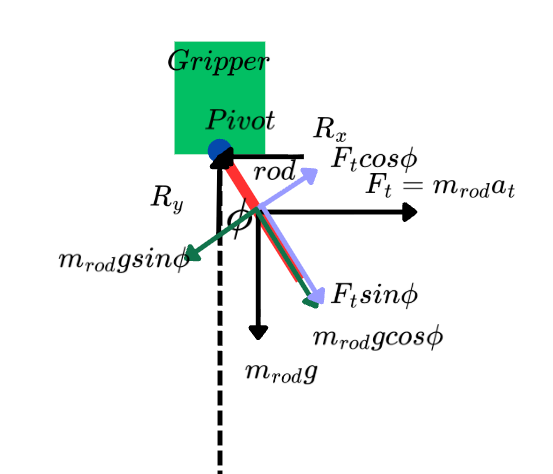
\includegraphics[width=0.65\textwidth]{fig_rod_pendulum_fbd}
    \caption{Free Body Diagram ของ Connection Rod จำลองเป็น Simple Pendulum
             ที่ถูกกระตุ้นด้วยความเร่งเชิงมุมของแขนกล}
    \label{fig:rod_pendulum_fbd}
\end{figure}
 
\subsubsection{สมการการเคลื่อนที่}
 
กำหนดให้ $\phi$ คือมุมเบี่ยงเบนของ Rod จากแนวดิ่ง (rad)
ในกรณี Small-Angle Approximation ($\sin\phi \approx \phi$)
สมการการเคลื่อนที่ของ Rod ในระบบอ้างอิงที่หมุนตามแขนกลได้จาก
 
\begin{equation}
    \ddot{\phi} + 2\zeta_{rod}\,\omega_{n,rod}\,\dot{\phi}
    + \omega_{n,rod}^2\,\phi = \Gamma\,\alpha_{arm}
    \label{eq:rod_eom}
\end{equation}
 
\noindent โดยที่ $\Gamma$ คือ Coupling Factor ระหว่างความเร่งแขนกลและการกระตุ้น Rod
และ $\alpha_{arm} = \ddot{\theta}_{arm}$ คือความเร่งเชิงมุมของแขนกล (rad/s²)
 
\subsubsection{การ Derive ความถี่ธรรมชาติ}
 
สำหรับ Rod ที่มีการกระจายมวลสม่ำเสมอตลอดความยาว $L_{rod}$
โมเมนต์ความเฉื่อยรอบจุดหมุนปลายคือ $I = \tfrac{1}{3}m_{rod}L_{rod}^2$
และ Restoring Torque คือ $\tau = -m_{rod}g\tfrac{L_{rod}}{2}\sin\phi$
จากสมการ $I\ddot{\phi} = \tau$ และ Small-Angle Approximation ได้
 
\begin{equation}
    \omega_{n,rod} = \sqrt{\frac{m_{rod}g\tfrac{L_{rod}}{2}}{\tfrac{1}{3}m_{rod}L_{rod}^2}}
                  = \sqrt{\frac{3g}{2L_{rod}}}
    \label{eq:rod_natural_freq}
\end{equation}
 
\noindent สำหรับ Connection Rod ในโครงงานนี้ที่มีความยาว $L_{rod} = 100$\,mm
 
\begin{equation}
    \omega_{n,rod} = \sqrt{\frac{3 \times 9.81}{2 \times 0.10}}
                  = \sqrt{147.15}
                  \approx 12.13\,\text{rad/s}
                  \quad (f_n \approx 1.93\,\text{Hz})
    \label{eq:rod_wn_num}
\end{equation}
 
\subsubsection{ความสำคัญต่อการออกแบบระบบควบคุม}
 
\cref{eq:rod_wn_num} แสดงว่า Rod มีความถี่ธรรมชาติต่ำมาก ($\approx 2$\,Hz)
เมื่อเทียบกับ Bandwidth ของ Position Loop (100\,Hz)
ดังนั้น Position PID ไม่สามารถ Damp การแกว่งของ Rod ได้
เพราะ Rod ไม่ได้อยู่ใน Feedback Loop ของ Controller
การแก้ปัญหาจึงต้องใช้ ZVD Input Shaper ที่ออกแบบให้ยกเลิกพลังงานที่ความถี่
$\omega_{n,rod}$ โดยตรงตามที่อธิบายใน\cref{subsec:zv_shaping}
\label{sec:trajectory}

% ============================================================================
\section{อัลกอริทึมสร้างโปรไฟล์การเคลื่อนที่}
\label{sec:trajectory}
% ============================================================================

\subsection{S-Curve Trajectory (Jerk-Limited)}
\label{subsec:scurve}

S-Curve Trajectory หรือ Jerk-Limited Trajectory เป็นโปรไฟล์การเคลื่อนที่ที่จำกัดอัตราการเปลี่ยนแปลงของความเร่ง (Jerk, $j = d^3\theta/dt^3$) ให้ไม่เกินค่าสูงสุด $j_{\max}$ ซึ่งช่วยลดแรงกระชากทางกล (Mechanical Shock) และจำกัดการกระตุ้นความถี่ธรรมชาติของระบบ เมื่อเทียบกับ Trapezoidal Profile ที่มีค่า Jerk เป็นอนันต์ ณ จุดที่เปลี่ยนความเร่ง

% -----------------------------------------------------------------------
% รูปที่ 6: กราฟ S-Curve Trajectory
% ชื่อไฟล์แนะนำ: fig_scurve_profile.pdf
% เนื้อหา: กราฟ 4 แกนซ้อนกันแนวตั้ง (Position, Velocity, Acceleration, Jerk) พร้อมเส้นประแบ่ง 7 เฟส
% -----------------------------------------------------------------------
\begin{figure}[H]
    \centering
    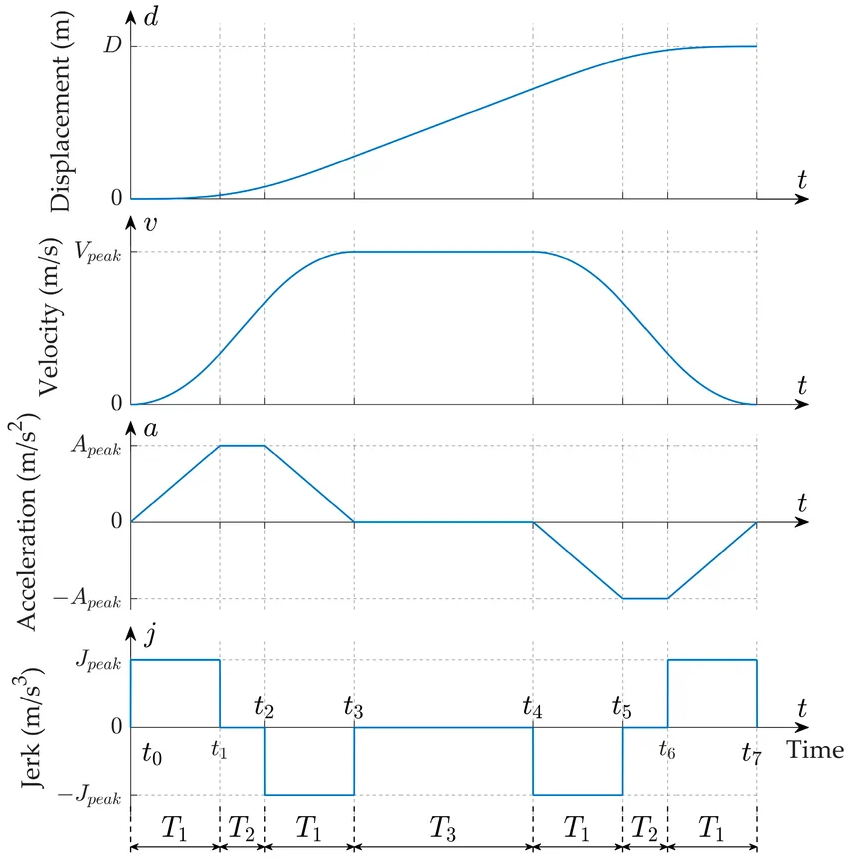
\includegraphics[width=0.9\textwidth]{fig_scurve_profile}
    \caption{โปรไฟล์การเคลื่อนที่แบบ S-Curve (Jerk-Limited) แสดงความสัมพันธ์เชิงจลนศาสตร์ทั้ง 7 เฟส}
    \label{fig:scurve_profile}
\end{figure}

\subsubsection{โครงสร้างเชิงเวลา (Time Intervals) ของ 7 เฟส}

การสร้าง S-Curve แบบสมมาตร (Symmetric Profile) สำหรับระยะทางเป้าหมาย $\Delta\theta$ จะประกอบด้วย 7 เฟส โดยมีสมการคำนวณระยะเวลาในแต่ละช่วง ($T_j, T_a, T_v$) เบื้องต้นดังนี้

\begin{align}
    T_j &= \frac{a_{\max}}{j_{\max}} \label{eq:scurve_tj} \\
    T_a &= \frac{v_{\max}}{a_{\max}} - T_j \label{eq:scurve_ta} \\
    T_v &= \frac{\Delta\theta}{v_{\max}} - (T_a + 2T_j) \label{eq:scurve_tv}
\end{align}

\noindent โดยที่:
\begin{itemize}
    \item \textbf{เฟส 1, 3, 5, 7 (Jerk Phases, $T_j$):} ช่วงที่ Jerk มีค่า $\pm j_{\max}$ เพื่อไต่ระดับหรือลดระดับความเร่ง
    \item \textbf{เฟส 2, 6 (Acceleration Phases, $T_a$):} ช่วงที่ความเร่งคงที่ $\pm a_{\max}$
    \item \textbf{เฟส 4 (Velocity Phase, $T_v$):} ช่วงที่ความเร็วคงที่ $v_{\max}$
\end{itemize}

\subsubsection{การพิจารณาสภาวะโปรไฟล์ไม่สมบูรณ์ (Partial Profiles)}

ในทางปฏิบัติ ระยะทาง $\Delta\theta$ อาจสั้นเกินกว่าที่ระบบจะเร่งไปถึง $v_{\max}$ หรือ $a_{\max}$ ได้ อัลกอริทึมจึงต้องตรวจสอบเงื่อนไขและคำนวณพารามิเตอร์ยอดแหลม (Peak Values) ใหม่ ดังนี้

\begin{itemize}
    \item \textbf{กรณีไม่ถึงความเร่งสูงสุด ($T_a \leq 0$):} ระบบจะถูกตัดเฟส 2 และ 6 ออก ความเร่งสูงสุดใหม่ที่ทำได้จะถูกจำกัดด้วย Jerk คือ $a_{reach} = \sqrt{v_{\max} j_{\max}}$
    \item \textbf{กรณีไม่ถึงความเร็วสูงสุด ($T_v \leq 0$):} ระบบจะถูกตัดเฟส 4 ออก และต้องคำนวณ $v_{reach}$ ใหม่จากสมการรากของระยะทางที่กำหนด
\end{itemize}

\subsubsection{ความสัมพันธ์กับ Cycle Time และ ZVD Shaper}

การกำหนดค่าพารามิเตอร์ต้องสอดคล้องกับข้อกำหนดของโครงงาน กล่าวคือ $v_{\max} \leq 5.84$\,rad/s (P3) และ $a_{\max} \leq 22.0$\,rad/s$^2$ (P4) เพื่อให้ Cycle Time รวมไม่เกิน 35 วินาที (P1)
ทั้งนี้ การใช้ S-Curve ทำหน้าที่เสมือน Pre-filter ที่ช่วยลดแอมพลิจูดของการแกว่งตั้งแต่ต้นทาง ส่งผลให้ ZVD Input Shaper ใน\cref{subsec:zv_shaping} รับภาระในการหักล้างการสั่นน้อยลง และลดโอกาสที่ Command จะทะลุขีดจำกัด Saturation ของวงจรควบคุมความเร็ว
% ============================================================================
\section{การระบุเอกลักษณ์ของระบบ (System Identification)}
\label{sec:system_id}
% ============================================================================

การนำแบบจำลอง State-Space ไปใช้งานจริงในตัวควบคุมและตัวประมาณค่าสถานะ (Kalman Filter) จำเป็นต้องทราบค่าพารามิเตอร์ทางกายภาพที่แม่นยำ ในโครงงานนี้ใช้แนวทาง Grey-Box Modeling โดยยึดโครงสร้างสมการทางฟิสิกส์เป็นหลัก แล้วหาค่าพารามิเตอร์จากการทดลองจริง

% ----------------------------------------------------------------------------
\subsection{การประมาณค่าพารามิเตอร์ทางไฟฟ้า (Stalled Rotor Test)}

เมื่อทำการล็อกเพลามอเตอร์ไม่ให้หมุน ($\omega = 0$) แรงเคลื่อนไฟฟ้าย้อนกลับ $e_b$ จะมีค่าเป็นศูนย์ 
ในการทดลองจะต่อตัวต้านทานชันต์ (Shunt Resistor, $R_{sh}$) อนุกรมเข้ากับมอเตอร์เพื่อใช้วัดกระแสทางอ้อมผ่านแรงดันตกคร่อม ($V_{sh}$) 
ตามกฎแรงดันของ Kirchhoff (KVL) จะได้สมการวงจรดังนี้

\begin{equation}
    V_{in} = i(t)\left(R_a + R_{sh}\right) + L_a \frac{di(t)}{dt}
    \label{eq:kvl_shunt}
\end{equation}

\noindent โดยที่ $V_{in}$ คือแรงดันแบบขั้นบันได (Step Voltage) ที่ป้อนเข้าสู่วงจร

\subsubsection{การหาค่าความต้านทานอาร์เมเจอร์ ($R_a$)}
เมื่อเวลาผ่านไปจนเข้าสู่สภาวะคงตัว (Steady State, $t \to \infty$) อัตราการเปลี่ยนแปลงของกระแสจะมีค่าเป็นศูนย์ ($di/dt = 0$) และกระแสไหลสูงสุด ($i_{ss}$) ซึ่งสามารถหาได้จากแรงดันที่ตกคร่อม Shunt Resistor ในสภาวะคงตัว ($V_{sh}$)

\begin{equation}
    V_{in} = i_{ss}\left(R_a + R_{sh}\right) \quad \text{โดยที่} \quad i_{ss} = \frac{V_{sh}}{R_{sh}}
\end{equation}

\noindent แทนค่า $i_{ss}$ และจัดรูปสมการเพื่อหา $R_a$ จะได้ความสัมพันธ์ดังนี้

\begin{equation}
    V_{in} = \frac{V_{sh}}{R_{sh}}\left(R_a + R_{sh}\right) \implies \frac{V_{in}}{V_{sh}} = \frac{R_a}{R_{sh}} + 1
\end{equation}

\begin{equation}
    R_a = R_{sh} \left( \frac{V_{in}}{V_{sh}} - 1 \right)
    \label{eq:calc_Ra}
\end{equation}

\subsubsection{การหาค่าความเหนี่ยวนำอาร์เมเจอร์ ($L_a$)}
การตอบสนองของกระแสในวงจร RL อนุกรม จะมีลักษณะเป็น First-order System ค่าคงที่เวลา (Time Constant, $\tau$) คือเวลาที่แรงดัน $V_{sh}$ ไต่ระดับขึ้นไปถึง 63.2\% ของค่าสูงสุดในสภาวะคงตัว โดยค่า $\tau$ ของวงจรนี้มีค่าเท่ากับ

\begin{equation}
    \tau = \frac{L_a}{R_{total}} = \frac{L_a}{R_a + R_{sh}}
\end{equation}

\noindent ดังนั้น $L_a = \tau(R_a + R_{sh})$ 
จากสภาวะคงตัวก่อนหน้า เราทราบว่า $(R_a + R_{sh}) = R_{sh}\frac{V_{in}}{V_{sh}}$ เมื่อนำมาแทนค่าจะได้สมการสำหรับคำนวณ $L_a$ ที่สามารถหาได้จากข้อมูลที่วัดได้โดยตรง

\begin{equation}
    L_a = R_{sh} \left( \tau \frac{V_{in}}{V_{sh}} \right)
    \label{eq:calc_La}
\end{equation}

% ----------------------------------------------------------------------------
\subsection{การระบุเอกลักษณ์แบบกล่องเทาด้วย MATLAB (Grey-Box Identification)}
\label{subsec:matlab_sysid}

แม้ว่าการหาพารามิเตอร์ด้วยวิธีล็อกเพลาและการหมุนตัวเปล่าจะให้ค่าประมาณการเบื้องต้น (Initial Guess) ที่อ้างอิงจากสมการทางฟิสิกส์ แต่ในสภาพแวดล้อมจริงระบบอาจมีความไม่เป็นเชิงเส้น (Non-linearities) เล็กน้อยแอบแฝงอยู่ 
โครงงานนี้จึงเลือกใช้ System Identification Toolbox ของซอฟต์แวร์ MATLAB เป็นเทคโนโลยีสำหรับปรับจูนค่าพารามิเตอร์ให้มีความแม่นยำสูงสุดผ่านกระบวนการหาค่าเหมาะสมที่สุด (Optimization)

\subsubsection{วิธีพยากรณ์ความคลาดเคลื่อน (Prediction Error Method: PEM)}
อัลกอริทึมของ MATLAB ทำงานโดยอาศัยหลักการลดรูปความคลาดเคลื่อนระหว่างผลตอบสนองของแบบจำลองคณิตศาสตร์ ($\hat{y}$) และข้อมูลที่วัดได้จริงจากเซนเซอร์ ($y$) โดยนิยามฟังก์ชันต้นทุน (Cost Function) ในรูปแบบของค่าผลรวมความผิดพลาดกำลังสอง (Sum of Squared Errors) ดังสมการ

\begin{equation}
    V_N(\mathbf{p}) = \frac{1}{N} \sum_{k=1}^N \left| y(k) - \hat{y}(k | \mathbf{p}) \right|^2
    \label{eq:pem_cost}
\end{equation}

\noindent โดยที่ $N$ คือจำนวนข้อมูลทั้งหมด (Samples) และ $\mathbf{p} = [R_a,\; L_a,\; K_t,\; J,\; B]^\top$ คือเวกเตอร์ของพารามิเตอร์อิสระ (Free Parameters) ที่ต้องการค้นหา

\subsubsection{กระบวนการประมวลผลอัลกอริทึม}
การประมาณค่าพารามิเตอร์แบบ Grey-Box บน MATLAB มีกลไกการทำงาน 3 ขั้นตอนหลัก ดังนี้
\begin{enumerate}
    \item \textbf{การสร้างแบบจำลอง (Model Definition):} กำหนดโครงสร้างเมทริกซ์ $\mathbf{A}, \mathbf{B}, \mathbf{C}, \mathbf{D}$ ของสมการ State-Space แบบ Continuous-Time ผ่านฟังก์ชันโครงสร้าง \texttt{idgrey} โดยป้อนค่าประมาณการเบื้องต้นที่ได้จากการคำนวณเชิงวิเคราะห์
    \item \textbf{การหาค่าเหมาะสมที่สุด (Parameter Estimation):} ป้อนข้อมูลอินพุต (แรงดัน $V_a$) และเอาต์พุต (กระแส $i_a$ และความเร็ว $\omega$) ที่บันทึกจากการทดลองจริงเข้าสู่ฟังก์ชัน \texttt{greyest} ซึ่งอัลกอริทึมจะใช้วิธีการค้นหาแบบไม่เป็นเชิงเส้น (Non-linear Least Squares) เช่น Levenberg-Marquardt ในการอัปเดตเวกเตอร์ $\mathbf{p}$ ซ้ำๆ (Iteration) จนกว่าฟังก์ชัน $V_N(\mathbf{p})$ จะลู่เข้าสู่ค่าจุดต่ำสุด (Convergence)
    \item \textbf{การตรวจสอบความถูกต้อง (Model Validation):} ประเมินความแม่นยำของแบบจำลองด้วยเปอร์เซ็นต์ความพอดี (Fit Percentage) ซึ่งคำนวณจากค่า Normalized Root Mean Square Error (NRMSE) ระหว่างกราฟผลตอบสนองจากการซิมูเลชัน (Simulated Output) และข้อมูลการวัดจริง (Measured Data)
\end{enumerate}

% % ----------------------------------------------------------------------------
% \subsection{การประมาณค่าพารามิเตอร์ทางกล (Free Run Test)}

% ในการทำงานที่สภาวะไม่มีโหลด ($\tau_d \approx 0$) และป้อนแรงดันคงที่จนมอเตอร์หมุนด้วยความเร็วคงตัว ($d\omega/dt = 0$) สมการโดเมนเชิงกลจะลดรูปลงเหลือ

% \begin{equation}
%     B\,\omega_{ss} = K_t\, i_{a,ss}
% \end{equation}

% \noindent ทำให้สามารถหาค่าสัมประสิทธิ์แรงหน่วงหนืด $B$ ได้จากการวัดกระแสและความเร็วรอบในสภาวะคงตัว สำหรับโมเมนต์ความเฉื่อย $J$ สามารถวิเคราะห์ได้จากการตอบสนองทางเวลา (Transient Response) และเวลาที่ใช้ในการเร่งความเร็ว (Rise Time) ของเพลา

% % ============================================================================
% \section{การขับกำลังมอเตอร์ด้วยสัญญาณ PWM}
% \label{sec:pwm_drive}
% % ============================================================================

% สัญญาณควบคุม $u$ ที่คำนวณจากตัวควบคุม PID จะถูกแปลงเป็นเปอร์เซ็นต์ Duty Cycle ($D \in [0, 1]$) เนื่องจากไมโครคอนโทรลเลอร์ไม่สามารถจ่ายแรงดันอนาล็อกกำลังสูงได้ จึงต้องทำงานร่วมกับวงจรขับมอเตอร์ (H-Bridge) สำหรับการขับแบบ Sign-Magnitude แรงดันอาร์เมเจอร์เฉลี่ยจะมีค่าเท่ากับ

% \begin{equation}
%     V_a = D \cdot V_{cc}
% \end{equation}

% \noindent โดยที่ $V_{cc}$ คือแรงดันจากแหล่งจ่ายกำลัง การเลือกความถี่ PWM ($f_{pwm}$) จะต้องสอดคล้องกับค่าคงที่เวลาทางไฟฟ้า ($\tau_e$) ของมอเตอร์ โดยทั่วไปควรกำหนดให้ $f_{pwm} \gg 1/\tau_e$ เพื่อให้วงจรอาร์เมเจอร์ทำหน้าที่เป็นตัวกรองสัญญาณความถี่ต่ำผ่าน (Low-Pass Filter) ได้อย่างสมบูรณ์ ป้องกันไม่ให้กระแสขาดตอน (Discontinuous Current Mode) และลดกระแสกระเพื่อม (Current Ripple)

% ----------------------------------------------------------------------------
\subsection{Zero-Phase Filtering ด้วย \texttt{filtfilt}}
\label{subsec:filtfilt}
% ----------------------------------------------------------------------------

ในงาน System Identification ข้อมูลที่บันทึกจาก Hardware
มักมีสัญญาณรบกวนความถี่สูงที่ต้องกำจัดออกก่อนนำเข้า Estimator
การกรองสัญญาณด้วย Digital Filter แบบทั่วไป (Causal Filter)
แม้จะลด Noise ได้ แต่มีผลข้างเคียงที่สำคัญคือ
\textbf{Phase Lag} ซึ่งส่งผลโดยตรงต่อความแม่นยำของพารามิเตอร์
ที่ประมาณได้

% ----------------------------------------------------------------------------
\subsubsection{ปัญหาของ Causal Filter: Phase Lag}

Causal Filter ประมวลผลข้อมูลจากอดีตไปปัจจุบันทิศทางเดียว
ทำให้ Output มี Phase Lag สัมพันธ์กับ Input
ที่ทุกความถี่ สำหรับ Butterworth Order~$n$ ที่ Cutoff $\omega_c$
Phase Response คือ

\begin{equation}
    \angle H(j\omega)
    = -n \arctan\!\left(\frac{\omega}{\omega_c}\right)
    \label{eq:butter_phase}
\end{equation}

ตัวอย่างเช่น Butterworth Order~4 ที่ $f_c = 10$\,Hz
มี Phase Lag ที่ $f = 1$\,Hz เท่ากับ

\begin{equation}
    \angle H(j2\pi \cdot 1)
    = -4\arctan\!\left(\frac{1}{10}\right)
    \approx -22.9\degree
    \label{eq:butter_phase_example}
\end{equation}

Phase Lag นี้ทำให้ข้อมูล Output ($\omega$) ล่าช้ากว่า
Input ($V_a$) ในชุดข้อมูลที่นำเข้า Estimator
Estimator จะพยายามปรับค่า Time Constant ของแบบจำลอง
ให้ตรงกับ Delay ที่เกิดจาก Filter แทนที่จะเป็น
Delay จากระบบจริง
ส่งผลให้พารามิเตอร์ที่ควบคุม Phase ของการตอบสนอง
โดยเฉพาะ $L_a$ และ $J$ มี \textbf{Bias Error}

% ----------------------------------------------------------------------------
\subsubsection{หลักการทำงานของ \texttt{filtfilt}}

\texttt{filtfilt} แก้ปัญหา Phase Lag ด้วยการประมวลผลข้อมูล
สองรอบในทิศทางตรงข้ามกัน ดังนี้

\begin{enumerate}
    \item \textbf{Forward Pass:}
          กรองข้อมูลจากต้นจนจบตามปกติ
          Output มี Phase Lag $-\phi(\omega)$
          และ Magnitude Response $|H(j\omega)|$

    \item \textbf{Backward Pass:}
          Reverse ลำดับ Output จาก Forward Pass
          แล้วกรองอีกครั้ง
          ซึ่งเทียบเท่ากับการกรองสัญญาณที่มี
          Phase $+\phi(\omega)$ อยู่แล้ว
          ผลที่ได้จึงมี Phase Lag สุทธิ
          $-\phi(\omega) + \phi(\omega) = 0$

    \item \textbf{Reverse กลับ:}
          Reverse ลำดับ Output จาก Backward Pass
          เพื่อให้ได้ข้อมูลที่เรียงลำดับถูกต้อง
\end{enumerate}

ผลลัพธ์คือสัญญาณที่มี \textbf{Zero-Phase Response}
ในทุกความถี่ แต่ Magnitude Response เทียบเท่ากับ
Filter เดิมยกกำลังสอง

\begin{equation}
    \left|H_{filtfilt}(j\omega)\right|
    = \left|H(j\omega)\right|^2
    = \frac{1}{\sqrt{1 + \left(\omega/\omega_c\right)^{2n}}}^{\,2}
    = \frac{1}{1 + \left(\omega/\omega_c\right)^{2n}}
    \label{eq:filtfilt_mag}
\end{equation}

กล่าวคือ Butterworth Order~4 เมื่อใช้ \texttt{filtfilt}
จะให้ Effective Order~8 และ Roll-off Rate $-160$\,dB/decade
ทำให้กำจัด Noise ได้รุนแรงขึ้นด้วย

% -----------------------------------------------------------------------
% รูปที่: filtfilt Zero-Phase Filtering
% ชื่อไฟล์แนะนำ: fig_filtfilt_concept.png
% เนื้อหา: กราฟ 3 แถวซ้อนกัน แกน X คือเวลา (s)
%   แถวบน:   Raw signal (สีเทา noisy) overlay กับ
%             Causal filter output (สีแดง) เห็น phase lag ชัดเจน
%   แถวกลาง: Raw signal (สีเทา) overlay กับ
%             filtfilt output (สีน้ำเงิน) ทับ peak ตรงๆ ไม่ lag
%   แถวล่าง: Causal (สีแดง) vs filtfilt (สีน้ำเงิน) overlay
%             พร้อม annotation ลูกศรชี้ phase difference
% สร้างด้วย MATLAB (run ใน command window):
%   fs = 1000; t = 0:1/fs:2;
%   x = sin(2*pi*1*t) + 0.3*randn(size(t));
%   [b,a] = butter(4, 10/(fs/2));
%   y_c = filter(b,a,x);
%   y_f = filtfilt(b,a,x);
%   figure('Color','w');
%   subplot(3,1,1); plot(t,x,'Color',[.7 .7 .7]); hold on;
%     plot(t,y_c,'r','LineWidth',1.5);
%     legend('Raw','Causal'); ylabel('Amplitude');
%   subplot(3,1,2); plot(t,x,'Color',[.7 .7 .7]); hold on;
%     plot(t,y_f,'b','LineWidth',1.5);
%     legend('Raw','filtfilt'); ylabel('Amplitude');
%   subplot(3,1,3); plot(t,y_c,'r','LineWidth',1.5); hold on;
%     plot(t,y_f,'b','LineWidth',1.5);
%     legend('Causal','filtfilt'); ylabel('Amplitude'); xlabel('Time (s)');
% -----------------------------------------------------------------------
\begin{figure}[H]
    \centering
    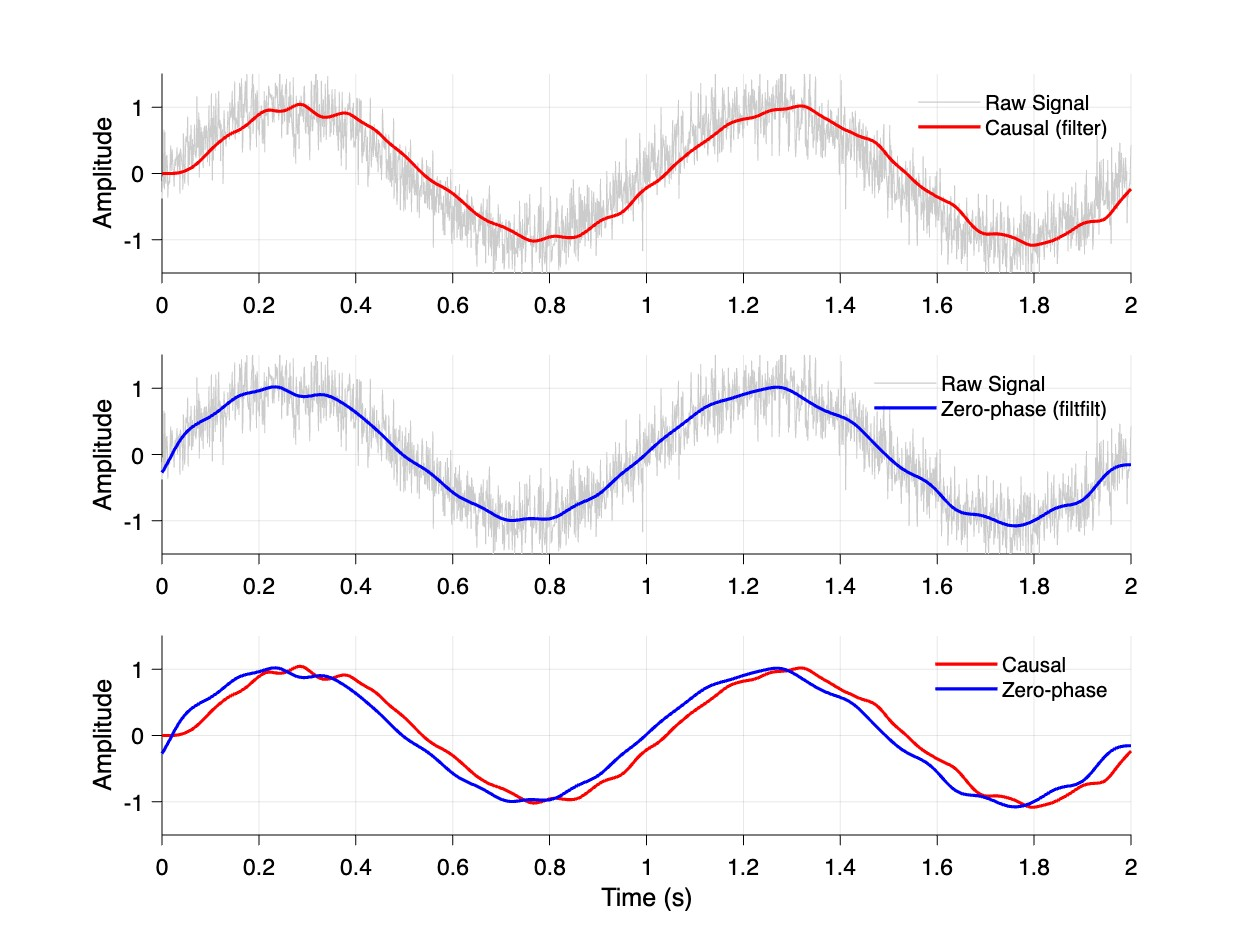
\includegraphics[width=0.90\textwidth]{fig_filtfilt_concept}
    \caption{เปรียบเทียบ Causal Filter (สีแดง) และ \texttt{filtfilt}
             Zero-Phase Filter (สีน้ำเงิน) บนสัญญาณเดียวกัน
             (บน) Causal Filter มี Phase Lag ที่สังเกตได้
             (กลาง) \texttt{filtfilt} ทับ Peak ของสัญญาณต้นฉบับได้ตรงทุกจุด
             (ล่าง) Phase Difference ระหว่างทั้งสองวิธี}
    \label{fig:filtfilt_concept}
\end{figure}

% ----------------------------------------------------------------------------
\subsubsection{ข้อจำกัดของ \texttt{filtfilt}}

เนื่องจากต้องใช้ข้อมูลทั้งชุดก่อนประมวลผล
\texttt{filtfilt} จึงเป็น \textbf{Offline Filter}
ไม่สามารถใช้งาน Real-time บน Embedded System ได้
ซึ่งเป็นที่ยอมรับได้ในบริบทของ System Identification
ที่ข้อมูลทั้งหมดถูกบันทึกไว้ก่อนแล้ว
สำหรับการใช้งานบน STM32G474RE ใน Closed-loop Control
จะใช้ Kalman Filter เป็น State Estimator แบบ Real-time
ตามที่อธิบายใน\cref{subsec:kalman_filter}
แทนการกรองสัญญาณโดยตรง

% ============================================================================
\section{ปรากฏการณ์อินทิกรัลไวนด์อัป (Integral Windup)}
\label{sec:integral_windup}
% ============================================================================

% -----------------------------------------------------------------------
% รูปที่ 12: กราฟแสดงปรากฏการณ์ Integral Windup และการแก้ปัญหาด้วย Back-Calculation
% แนะนำให้เปลี่ยนชื่อไฟล์ภาพเป็น fig_integral_windup.png ก่อนนำไปใช้งาน
% -----------------------------------------------------------------------
\begin{figure}[H]
    \centering
    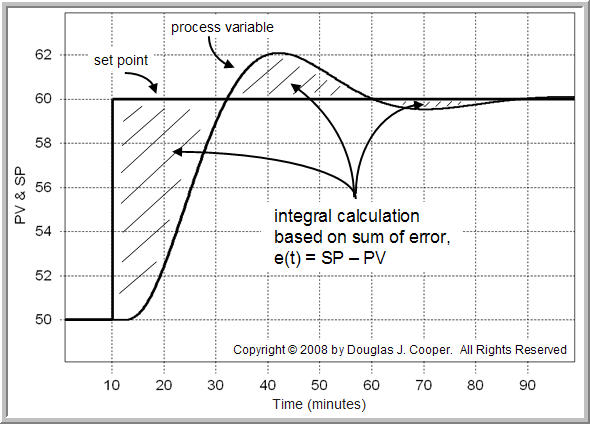
\includegraphics[width=0.7\textwidth]{fig_integral_windup}
    \caption{การเปรียบเทียบการตอบสนองของระบบ (บน) สัญญาณควบคุม (กลาง) และการสะสมสถานะของตัวอินทิเกรต (ล่าง) ระหว่างตัวควบคุม PID มาตรฐานและตัวควบคุมที่มีการติดตั้งระบบ Anti-Windup แบบ Back-Calculation}
    \label{fig:integral_windup}
\end{figure}

ในระบบควบคุมจริง อุปกรณ์ขับกำลัง (เช่น H-Bridge) มีขีดจำกัดการจ่ายแรงดันสูงสุด (Saturation Limit, $u_{\max}$) หากระบบเกิดความคลาดเคลื่อนสะสมเป็นเวลานาน เทอมอินทิกรัล ($K_i \int e \,dt$) จะมีค่าเพิ่มขึ้นเรื่อยๆ จนเกินความสามารถของอุปกรณ์ ปรากฏการณ์นี้เรียกว่า Integral Windup ซึ่งส่งผลให้ระบบมีการตอบสนองที่ล่าช้าเมื่อความคลาดเคลื่อนเปลี่ยนทิศทาง และทำให้เกิด Overshoot ขนาดใหญ่

ดังที่ได้แสดงสมการการทำงานของระบบ Anti-Windup แบบ Back-Calculation ไว้ใน\cref{eq:anti_windup} อัลกอริทึมจะป้อนกลับส่วนต่างระหว่างคำสั่งก่อนจำกัด (Unsaturated Command) และหลังจำกัด (Saturated Command) มาลดทอนสถานะของ Integrator แบบ Real-time เพื่อรักษาระบบให้อยู่ในขอบเขตเชิงเส้น

% ============================================================================
\section{มาตรฐานตู้ควบคุมอุตสาหกรรม (Industrial Enclosures)}
\label{sec:industrial_standards}
% ============================================================================

% การนำระบบควบคุมหุ่นยนต์ไปใช้งานในสภาพแวดล้อมคลังสินค้า (Warehouse Environment) ตู้ควบคุม (Control Cabinet) จะต้องได้รับการออกแบบให้ทนทานต่อสภาวะแวดล้อมและมีความปลอดภัยทางไฟฟ้าตามมาตรฐานอุตสาหกรรม การออกแบบตู้ควบคุมที่ดีไม่เพียงแต่ปกป้องฮาร์ดแวร์ภายใน แต่ยังช่วยลดปัญหาสัญญาณรบกวนและยืดอายุการใช้งานของระบบ

% \subsection{การป้องกันสิ่งแปลกปลอม (Ingress Protection: IEC 60529)}
% การปกป้องแผงวงจรและอุปกรณ์อิเล็กทรอนิกส์จากฝุ่นละอองและน้ำอ้างอิงตามมาตรฐาน IEC 60529 (IP Rating) ในสภาพแวดล้อมคลังสินค้าทั่วไป มักกำหนดระดับการป้องกันขั้นต่ำที่ IP54
% \begin{itemize}
%     \item \textbf{เลขหลักแรก (Solid Particle Protection):} ระดับ 5 หมายถึงป้องกันฝุ่นละอองได้ในระดับที่ฝุ่นไม่สามารถเข้าไปรบกวนการทำงานและทำให้เกิดการลัดวงจรของอุปกรณ์
%     \item \textbf{เลขหลักที่สอง (Liquid Ingress Protection):} ระดับ 4 หมายถึงป้องกันละอองน้ำที่กระเด็นมาจากทุกทิศทาง
% \end{itemize}
% อย่างไรก็ตาม การเพิ่มระดับการป้องกันที่สูงกว่านี้ (เช่น IP65) จะทำให้ตู้เป็นระบบปิดสมบูรณ์แบบ ซึ่งส่งผลกระทบโดยตรงต่อการระบายความร้อน จึงต้องมีการวิเคราะห์การจัดการทางความร้อนควบคู่กันเสมอ

% \subsection{การจัดการความร้อน (Thermal Management)}
% อุปกรณ์ขับกำลัง (Motor Driver) และหน่วยประมวลผลแบบ Edge AI มีการคายความร้อน (Heat Dissipation) ระหว่างทำงาน หากตู้ควบคุมเป็นระบบปิด ความร้อนสะสมจะทำให้อุณหภูมิภายในพุ่งสูงขึ้น อุณหภูมิที่เพิ่มขึ้น ($\Delta T$) สามารถประเมินได้จากสมการสมดุลความร้อน

% \begin{equation}
%     \Delta T = \frac{P_{loss}}{U \cdot A}
%     \label{eq:enclosure_temp}
% \end{equation}

% \noindent โดยที่ $P_{loss}$ คือกำลังงานสูญเสียรวมของอุปกรณ์ภายใน (\si{\watt}), $U$ คือสัมประสิทธิ์การถ่ายเทความร้อนของวัสดุตู้ (\si{\watt\per\metre\squared\per\kelvin}) (เช่น แผ่นเหล็กพ่นสีมีค่าประมาณ 5.5) และ $A$ คือพื้นที่ผิวสัมผัสอากาศของตู้ควบคุม (\si{\metre\squared}) 
% หากผลรวมอุณหภูมิแวดล้อมกับ $\Delta T$ มีค่าเกินกว่าอุณหภูมิการทำงานสูงสุด (Maximum Operating Temperature) ของอุปกรณ์ จะต้องพิจารณาติดตั้งพัดลมระบายอากาศพร้อมฟิลเตอร์กันฝุ่น (Filter Fan) หรือแผ่นระบายความร้อน (Heatsink)

\subsection{การจัดการสายไฟและลดสัญญาณรบกวน (Wiring \& EMI Mitigation)}
การออกแบบการจัดวางสายไฟอ้างอิงตามมาตรฐานความปลอดภัยของเครื่องจักร IEC 60204-1 โดยยึดรางอุปกรณ์มาตรฐาน (DIN 35mm) และมีหลักการจัดการคลื่นแม่เหล็กไฟฟ้าแทรกสอด (Electromagnetic Interference: EMI) ดังนี้
\begin{itemize}
    \item \textbf{Cable Segregation:} สายไฟฟ้ากำลัง (Power Cables) และสายสัญญาณ (Signal Cables) จะต้องถูกแยกเดินในรางเก็บสาย (Wire Duct) ที่ต่างกัน โดยมีระยะห่างอย่างน้อย 50 มิลลิเมตร หากมีความจำเป็นต้องเดินสายพาดผ่านกัน จะต้องจัดวางให้ตัดกันแบบตั้งฉาก ($90\degree$) เพื่อลดค่าความเหนี่ยวนำร่วม (Mutual Inductance) ให้เหลือน้อยที่สุด
    \item \textbf{Shielding \& Grounding:} สายสัญญาณแอนะล็อกและสายสื่อสาร (เช่น CAN Bus) ต้องใช้สายคู่ตีเกลียวมีชิลด์ (Shielded Twisted Pair) และจุดต่อสายดิน (Grounding) ของระบบควบคุมทั้งหมดต้องเชื่อมต่อรวมกันแบบจุดเดียว (Star Grounding) เพื่อป้องกันการเกิดลูปของสายดิน (Ground Loop) ที่จะสร้างความต่างศักย์รบกวนสัญญาณเซนเซอร์
\end{itemize}

\subsection{ความปลอดภัยทางไฟฟ้าและวงจรหยุดฉุกเฉิน (Electrical Safety \& E-Stop)}
ภายในตู้ควบคุมต้องติดตั้งอุปกรณ์ป้องกันกระแสเกิน (Overcurrent Protection) เช่น เบรกเกอร์ (MCB) หรือฟิวส์ ที่มีพิกัดสอดคล้องกับขนาดหน้าตัดของสายไฟ นอกจากนี้ หุ่นยนต์เคลื่อนที่อัตโนมัติต้องมีวงจรหยุดฉุกเฉิน (Emergency Stop) ระดับฮาร์ดแวร์ โดยสวิตช์ E-Stop ต้องต่ออนุกรมเพื่อตัดแหล่งจ่ายไฟออกจากอุปกรณ์ขับกำลัง (Actuators) โดยตรง (Hard-wired) โดยไม่พึ่งพาการประมวลผลทางซอฟต์แวร์เพียงอย่างเดียว เพื่อรับประกันความปลอดภัยเมื่อไมโครคอนโทรลเลอร์เกิดการค้าง (System Hang)

% ============================================================================
\section{การออกแบบระบบไฟฟ้าและวงจรป้องกัน (Electrical System and Protection Design)}
\label{sec:electrical_protection}
% ============================================================================

การออกแบบฮาร์ดแวร์สำหรับหุ่นยนต์อัตโนมัติ ไม่เพียงแต่ต้องพิจารณาด้านประสิทธิภาพการประมวลผล แต่ยังต้องคำนึงถึงเสถียรภาพของระบบจ่ายกำลังและการป้องกันความเสียหายจากสภาวะผิดปกติทางไฟฟ้า โดยอ้างอิงหลักการออกแบบวงจรสำหรับระบบหุ่นยนต์ระดับอุตสาหกรรม ดังนี้

\subsection{วงจรป้องกันความผิดปกติทางไฟฟ้า (Electrical Protection Circuits)}
ในระบบที่ต้องจัดการกับกระแสไฟฟ้าสูงและอุปกรณ์ทางกล มีความเสี่ยงที่จะเกิดความผิดปกติทางไฟฟ้าซึ่งอาจทำลายหน่วยประมวลผลหลักได้ การออกแบบจึงต้องมีมาตรการป้องกันใน 3 ระดับ:

\begin{itemize}
    \item \textbf{การป้องกันกระแสเกิน (Overcurrent Protection):} การใช้งานฟิวส์ (Fuses) หรือฟิวส์แบบตั้งค่าใหม่ได้ (PTC Resettable Fuses) ต่ออนุกรมในวงจรแหล่งจ่ายกำลัง เพื่อตัดวงจรเมื่อกระแสโหลดเกินพิกัด (Overload) หรือเกิดการลัดวงจร (Short Circuit) ป้องกันความร้อนสะสมที่อาจทำให้สายไฟหลอมละลายหรือเกิดเพลิงไหม้
    \item \textbf{การป้องกันการต่อสลับขั้ว (Reverse Polarity Protection):} การใช้ไดโอดกำลัง (Power Diode) แบบชอตต์กี (Schottky Diode) หรือวงจร P-Channel MOSFET เพื่อป้องกันกระแสไหลย้อนกลับเข้าไปทำลายแผงวงจรหลัก ในกรณีที่มีการต่อขั้วแบตเตอรี่หรือจุดเชื่อมต่อแหล่งจ่ายไฟสลับขั้ว
    \item \textbf{การป้องกันแรงดันกระชาก (Transient Voltage Suppression):} มอเตอร์กระแสตรงมีคุณสมบัติเป็นโหลดทางเหนี่ยวนำ (Inductive Load) เมื่อมีการตัดต่อกระแสไฟฟ้าอย่างรวดเร็ว (เช่น สัญญาณ PWM) หรือเมื่อเกิดสภาวะหยุดกะทันหัน จะเกิดแรงดันเหนี่ยวนำย้อนกลับ (Inductive Kickback) การติดตั้งตัวต้านทานแรงดันกระชาก (TVS Diode) ขนานกับสายไฟกำลัง จะช่วยขริบแรงดันกระชาก (Voltage Clamping) ไม่ให้ทะลุขีดจำกัดแรงดันของอุปกรณ์เซมิคอนดักเตอร์
\end{itemize}

\subsection{การแยกกัลวานิกทางแสง (Galvanic Isolation)}

% -----------------------------------------------------------------------
% รูปที่ 8: การแยกกัลวานิกด้วย Optocoupler
% ชื่อไฟล์แนะนำ: fig_galvanic_isolation.pdf
% เนื้อหา: Block diagram แสดงการแยก Ground ระหว่างภาค Logic และภาค Power อย่างเด็ดขาด
% -----------------------------------------------------------------------
\begin{figure}[H]
    \centering
    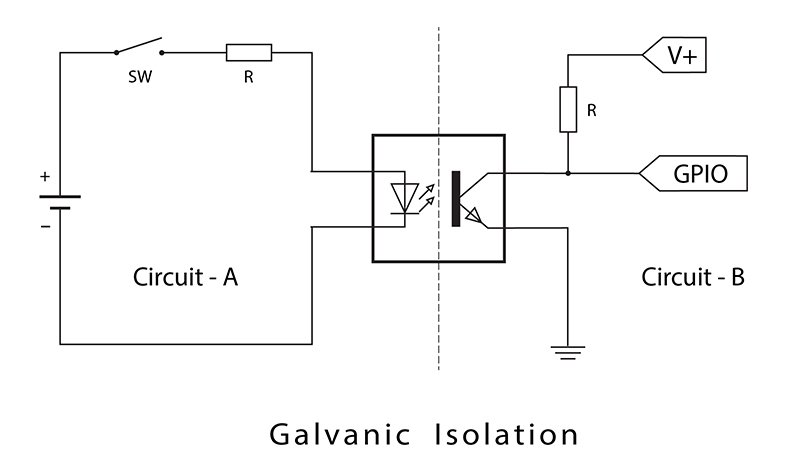
\includegraphics[width=0.75\textwidth]{fig_galvanic_isolation}
    \caption{หลักการแยกกัลวานิกทางแสง (Galvanic Isolation) เพื่อป้องกันสัญญาณรบกวนจากภาคขับกำลังไหลกลับเข้าสู่ภาคตรรกะ}
    \label{fig:galvanic_isolation}
\end{figure}

ระบบควบคุมหุ่นยนต์จำเป็นต้องแยกสภาวะทางไฟฟ้าระหว่าง "วงจรลอจิกแรงดันต่ำ" (Low-Voltage Logic เช่น MCU 3.3V/5V) และ "วงจรขับกำลังแรงดันสูง" (High-Power Drive เช่น Motor 24V) ออกจากกันอย่างเด็ดขาด โครงงานนี้ใช้ ออปโตคัปเปลอร์ (Optocouplers หรือ Optoisolators) ในการส่งผ่านสัญญาณ PWM จากไมโครคอนโทรลเลอร์ไปยัง H-Bridge ผ่านแสงอินฟราเรด ซึ่งช่วยป้องกันไม่ให้สัญญาณรบกวน (Noise) และแรงดันกระชากจากฝั่งมอเตอร์ไหลกลับมาทำลายหน่วยประมวลผลหลัก แม้ว่าอุปกรณ์ขับกำลังจะเกิดความเสียหายรุนแรงก็ตาม

\subsection{การจัดการสายไฟและหน้าสัมผัส (Wiring and Strain Relief)}
ความต้านทานแฝงและความเค้นทางกลในระบบสายไฟ เป็นสาเหตุหลักที่ทำให้หุ่นยนต์ทำงานผิดพลาด
\begin{itemize}
    \item \textbf{ขนาดพิกัดสายไฟ (Wire Gauge):} การเลือกขนาดหน้าตัดสายไฟตามมาตรฐาน AWG (American Wire Gauge) ต้องสอดคล้องกับพิกัดกระแสไฟฟ้าสูงสุด โดยสายกำลังของมอเตอร์ (Power Lines) ต้องมีค่า AWG ต่ำ (หน้าตัดใหญ่) เพื่อลดค่าความต้านทานและกำลังสูญเสียในรูปความร้อน ($I^2R$) ในขณะที่สายสัญญาณ (Signal Lines) สามารถใช้สาย AWG สูง (หน้าตัดเล็ก) เพื่อความยืดหยุ่นได้
    \item \textbf{จุดเชื่อมต่อและการลดความเค้น (Connectors \& Strain Relief):} บริเวณจุดเชื่อมต่อระหว่างบอร์ด PCB และสายไฟภายนอก จะต้องใช้คอนเนกเตอร์ที่ทนกระแสสูงและมีการล็อกทางกล (Mechanical Lock) อย่างแน่นหนา รวมถึงการออกแบบตัวลดความเค้นสายไฟ (Strain Relief) เพื่อป้องกันการขยับตัวที่อาจทำให้จุดบัดกรีฉีกขาด (Solder Joint Fatigue) ระหว่างที่กลไกของหุ่นยนต์มีการเคลื่อนที่และสั่นสะเทือน
\end{itemize}

% ============================================================================
\section{โพรโทคอลการสื่อสารข้อมูลอุตสาหกรรม}
\label{sec:communication_protocols}
% ============================================================================

การแลกเปลี่ยนข้อมูลระหว่าง Node ประมวลผล ระบบ Edge AI และอุปกรณ์ระดับล่าง (Sensors/Actuators) จำเป็นต้องใช้โครงข่ายการสื่อสารที่มีความน่าเชื่อถือสูงและทนทานต่อสภาพแวดล้อมทางอุตสาหกรรมที่มีสัญญาณรบกวนทางแม่เหล็กไฟฟ้า (EMI) หนาแน่น

% ----------------------------------------------------------------------------
\subsection{Controller Area Network (CAN Bus)}

CAN Bus เป็นโพรโทคอลแบบอนุกรมที่ถูกออกแบบมาสำหรับระบบยานยนต์และหุ่นยนต์โดยเฉพาะ ตามมาตรฐาน ISO 11898


\subsubsection{หลักการทำงานเชิงลึกและกลไกการเข้าถึงบัส}
ชั้นกายภาพ (Physical Layer) ของ CAN ใช้สายคู่ตีเกลียวส่งสัญญาณแบบผลต่าง (Differential Signaling) ผ่านสาย CAN\_H และ CAN\_L โดยกำหนดสถานะลอจิกเป็นสองระดับ ได้แก่
\begin{itemize}
    \item \textbf{Dominant State (ลอจิก '0'):} สาย CAN\_H มีแรงดันสูงกว่า CAN\_L ($V_{diff} \approx 2.0\text{V}$)
    \item \textbf{Recessive State (ลอจิก '1'):} สาย CAN\_H และ CAN\_L มีแรงดันเท่ากัน ($V_{diff} \approx 0\text{V}$)
\end{itemize}

% -----------------------------------------------------------------------
% รูปที่แนะนำ: แสดงกลไก Arbitration ของ CAN Bus
% ชื่อไฟล์แนะนำ: fig_can_arbitration.pdf
% เนื้อหา: แผนภาพแสดง Node A และ Node B ส่งข้อมูลพร้อมกัน และ Node ที่ส่งบิต '1' (Recessive) จะพ่ายแพ้ให้กับบิต '0' (Dominant)
% -----------------------------------------------------------------------
% \begin{figure}[H]
%     \centering
%     \includegraphics[width=0.85\textwidth]{fig_can_arbitration}
%     \caption{กลไก Bit-wise Arbitration ของ CAN Bus ที่ให้สิทธิ์ Node ที่มี ID ต่ำกว่าสามารถยึดบัสได้โดยข้อมูลไม่สูญหาย}
%     \label{fig:can_arbitration}
% \end{figure}

% -----------------------------------------------------------------------
% รูปที่ 9: ระดับแรงดันของสัญญาณ CAN Bus
% ชื่อไฟล์แนะนำ: fig_can_voltage_levels.pdf
% เนื้อหา: กราฟแสดงผลต่างแรงดันระหว่างสาย CAN_H และ CAN_L ในสถานะ Dominant และ Recessive
% -----------------------------------------------------------------------
\begin{figure}[H]
    \centering
    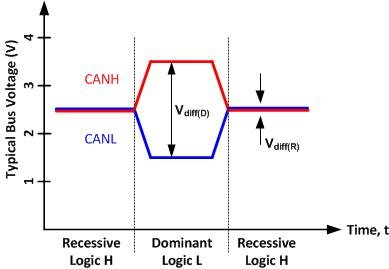
\includegraphics[width=0.8\textwidth]{fig_can_voltage_levels}
    \caption{ลักษณะทางกายภาพของสัญญาณ CAN Bus แสดงผลต่างแรงดันในการกำหนดสถานะตรรกะแบบ Dominant และ Recessive}
    \label{fig:can_voltage_levels}
\end{figure}

กลไกจัดการการชนกันของข้อมูลใช้เทคนิค \textbf{CSMA/CD+AMP} (Carrier Sense Multiple Access / Collision Detection with Arbitration on Message Priority) เมื่อมีหลาย Node พยายามส่งข้อมูลพร้อมกัน บัสจะทำการเปรียบเทียบรหัสประจำตัว (Message ID) ทีละบิต (Bit-wise Arbitration) หาก Node ใดส่งสถานะ Recessive ('1') แต่ตรวจพบว่าบัสอยู่ในสถานะ Dominant ('0') จาก Node อื่น Node นั้นจะหยุดส่งข้อมูลทันทีและเปลี่ยนเป็นผู้รับ ส่งผลให้ Message ID ที่มีค่าน้อยที่สุดจะมีความสำคัญสูงสุด (Highest Priority) และสามารถยึดบัสได้โดยที่เฟรมข้อมูลไม่เกิดการสูญหาย

% \subsubsection{ความเหมาะสมต่อระบบหุ่นยนต์}
% CAN Bus เหมาะสมอย่างยิ่งสำหรับโครงสร้างการควบคุมแบบกระจายศูนย์ (Distributed Control) เช่น การสื่อสารระหว่างตัวควบคุมหลัก (Main Controller) และตัวขับมอเตอร์ (Motor Drivers) ในแต่ละข้อต่อของหุ่นยนต์ เนื่องจากรองรับสถาปัตยกรรมแบบ Multi-Master ทำให้ทุก Node สามารถริเริ่มการส่งข้อมูลได้ทันทีเมื่อเกิดเหตุการณ์สำคัญ (Event-Driven) และให้ความแน่นอนทางเวลา (Real-time Determinism) สูง

% ----------------------------------------------------------------------------
\subsection{ชั้นกายภาพ RS-485 และโพรโทคอล Modbus RTU}

ในขณะที่ CAN Bus เหมาะสำหรับระบบภายในตัวหุ่นยนต์ การสื่อสารระยะไกลกับอุปกรณ์อุตสาหกรรมภายนอก (เช่น เซนเซอร์ระยะทาง, PLC, หรืออุปกรณ์ในคลังสินค้า) มักอาศัยมาตรฐาน RS-485 ร่วมกับ Modbus RTU

\subsubsection{หลักการทำงานของ UART และ RS-485}
ไมโครคอนโทรลเลอร์ประมวลผลข้อมูลผ่านฮาร์ดแวร์ UART (Universal Asynchronous Receiver-Transmitter) ซึ่งจัดข้อมูลในรูปของเฟรม ประกอบด้วย Start Bit, Data Bits (8 บิต), Parity Bit (ทางเลือก) และ Stop Bit แต่เนื่องจากสัญญาณ UART เป็นแบบ Single-Ended (อ้างอิงกับกราวด์) จึงมีข้อจำกัดด้านระยะทางและอ่อนไหวต่อสัญญาณรบกวน 

เพื่อแก้ปัญหานี้ สัญญาณ UART จะถูกแปลงผ่าน Transceiver ให้เข้าสู่มาตรฐาน \textbf{RS-485} ซึ่งส่งสัญญาณแบบผลต่าง (Differential) ตามสมการ:
\begin{equation}
    V_{diff} = V_A - V_B
\end{equation}
\noindent หาก $V_A - V_B > +200\text{mV}$ ตัวรับจะอ่านค่าเป็นลอจิก '1' และหาก $V_A - V_B < -200\text{mV}$ จะอ่านเป็นลอจิก '0' การใช้ผลต่างแรงดันนี้ทำให้สามารถส่งข้อมูลได้ไกลสูงสุดถึง 1,200 เมตร และหักล้างสัญญาณรบกวนที่เหนี่ยวนำเข้ามาพร้อมกันทั้งสองเส้น (Common-Mode Noise Rejection)

\subsubsection{กลไกของ Modbus RTU}
Modbus RTU ทำงานในชั้น Application Layer บนโครงข่าย RS-485 ด้วยสถาปัตยกรรมแบบ \textbf{Master-Slave} โดยอุปกรณ์ Master เพียงตัวเดียวจะเป็นผู้สั่งการ (Polling) และ Slave จะตอบสนองเมื่อถูกเรียกตาม Address ของตนเท่านั้น ป้องกันปัญหาการชนกันของข้อมูลโดยเด็ดขาด 

เฟรมข้อมูลของ Modbus RTU มีการต่อท้ายด้วยรหัส \textbf{CRC-16 (Cyclic Redundancy Check)} ซึ่งเป็นการหารพหุนาม (Polynomial Division) ระดับบิต เพื่อตรวจสอบความสมบูรณ์ของข้อมูลทั้งหมดในแพ็กเกจ หากฝั่งรับคำนวณ CRC ได้ไม่ตรงกับที่แนบมา ข้อมูลชุดนั้นจะถูกเพิกเฉยเพื่อป้องกันพฤติกรรมผิดพลาดของ Actuator

% -----------------------------------------------------------------------
% รูปที่ 11: โครงสร้างแพ็กเกจข้อมูล Modbus RTU
% ชื่อไฟล์แนะนำ: fig_modbus_frame.pdf
% เนื้อหา: แผนภาพแสดงไบต์ข้อมูลภายในเฟรม Modbus RTU โดยเน้นย้ำตำแหน่งของ CRC
% -----------------------------------------------------------------------
\begin{figure}[H]
    \centering
    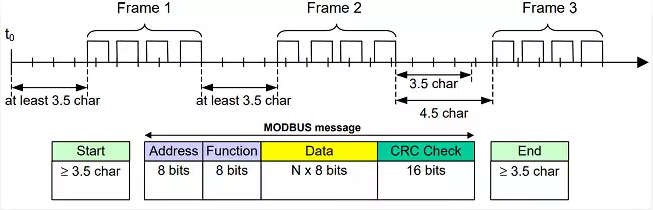
\includegraphics[width=0.85\textwidth]{fig_modbus_frame}
    \caption{โครงสร้างเฟรมข้อมูลของโพรโทคอล Modbus RTU แสดงการจัดเรียงไบต์ข้อมูลและรหัสตรวจสอบความผิดพลาด (CRC-16)}
    \label{fig:modbus_frame}
\end{figure}

% \subsubsection{ความเหมาะสมต่อระบบหุ่นยนต์}
% โครงสร้าง Master-Slave ของ Modbus RTU แม้จะมีความล่าช้า (Latency) จากวงรอบการ Polling แต่มีความน่าเชื่อถือสูงมาก และเป็นมาตรฐานที่พบได้ทั่วไปในอุปกรณ์อุตสาหกรรม จึงเหมาะสมสำหรับการเชื่อมต่อระหว่างระบบจัดการส่วนกลาง (Edge AI หรือ Warehouse Control System) กับอุปกรณ์โครงสร้างพื้นฐาน

        % % ----------------------------------------------------------------------------
        % \subsection{การสื่อสารไร้สาย Bluetooth (IEEE 802.15.1)}
        % สำหรับการควบคุมแบบมนุษย์อยู่ในวงรอบ (Human-in-the-loop) ผ่านอุปกรณ์จอยสติ๊กไร้สาย โครงงานนี้เลือกใช้มาตรฐาน Bluetooth ซึ่งทำงานในย่านความถี่ ISM Band (2.4 GHz) 

        % \subsubsection{เทคนิค Adaptive Frequency Hopping (AFH)}
        % เนื่องจากย่านความถี่ 2.4 GHz เป็นย่านสาธารณะที่มีการรบกวนสูง (เช่น จาก Wi-Fi ในพื้นที่) มาตรฐาน Bluetooth ได้แก้ไขปัญหานี้ด้วยเทคนิค \textbf{AFH} ซึ่งอัลกอริทึมจะประเมินคุณภาพของช่องสัญญาณ (Channel Assessment) เพื่อสร้างแผนที่ช่องสัญญาณที่ใช้งานได้ (Channel Map) จากนั้นตัวส่งและตัวรับจะกระโดดสลับความถี่ (Frequency Hopping) ไปยังช่องสัญญาณที่ว่างในอัตรา 1,600 ครั้งต่อวินาที (ทุกๆ 625 ไมโครวินาที)

        % \subsubsection{ความเหมาะสมต่อระบบ}
        % ความสามารถในการหลบหลีกสัญญาณรบกวนแบบพลวัต (Dynamic Interference Avoidance) ทำให้ Bluetooth มีเสถียรภาพเพียงพอสำหรับการส่งคำสั่งควบคุมทิศทางแบบเรียลไทม์ (Teleoperation) ภายในระยะทำการของตัวหุ่นยนต์ โดยไม่ถูกตัดขาดแม้ทำงานในสภาพแวดล้อมที่มีสัญญาณวิทยุหนาแน่น
        % % \subsection{การสื่อสารไร้สาย Bluetooth (IEEE 802.15.1)}
        % % สำหรับการควบคุมแบบมนุษย์อยู่ในวงรอบ (Human-in-the-loop) ผ่านอุปกรณ์จอยสติ๊ก (Joystick) โครงงานนี้เลือกใช้การสื่อสารไร้สายผ่านมาตรฐาน Bluetooth ซึ่งทำงานในย่านความถี่ ISM Band (2.4 GHz) 
        % % แม้ว่าย่านความถี่นี้จะมีการใช้งานหนาแน่นและมีโอกาสเกิดสัญญาณรบกวน (Interference) จากระบบ Wi-Fi ในพื้นที่ แต่มาตรฐาน Bluetooth ได้แก้ไขปัญหานี้ด้วยเทคนิค \textbf{Adaptive Frequency Hopping (AFH)} ซึ่งอัลกอริทึมจะทำการประเมินคุณภาพของช่องสัญญาณ (Channel Assessment) อย่างต่อเนื่อง และทำการกระโดดสลับความถี่ (Hopping) ไปยังช่องสัญญาณที่ว่างหรือมีสัญญาณรบกวนต่ำในอัตรา 1,600 ครั้งต่อวินาที ทำให้มีความน่าเชื่อถือเพียงพอสำหรับการส่งคำสั่งควบคุม (Control Command) เข้าสู่ระบบ

% ============================================================================
\section{เซนเซอร์และอุปกรณ์ตรวจวัด}
\label{sec:sensors}
% ============================================================================
 
ระบบใช้เซนเซอร์สามประเภทที่ทำงานร่วมกัน
ได้แก่ Encoder สำหรับวัดตำแหน่ง, Current Sensor สำหรับตรวจสอบความปลอดภัย
และ Proximity Sensor สำหรับกำหนดจุด Home
 
% ----------------------------------------------------------------------------
\subsection{Incremental Encoder (AMT-103)}
\label{subsec:encoder_theory}
 
Incremental Encoder วัดการเปลี่ยนแปลงตำแหน่งเชิงมุมโดยนับพัลส์
จาก Quadrature Signal สองช่อง (Channel A และ Channel B)
ที่มีเฟสต่างกัน $90\degree$ ทำให้สามารถระบุทิศทางการหมุนได้
 
% -----------------------------------------------------------------------
% รูปที่ X: Encoder AMT-103 และ Quadrature Signal
% ชื่อไฟล์แนะนำ: fig_encoder_quadrature.pdf
% เนื้อหา: แสดงรูป AMT-103 (ซ้าย) และ Timing Diagram ของ CH A, CH B, Index (ขวา)
%          พร้อม annotation ทิศทาง CW/CCW จากลำดับ edge
% -----------------------------------------------------------------------
\begin{figure}[H]
    \centering
    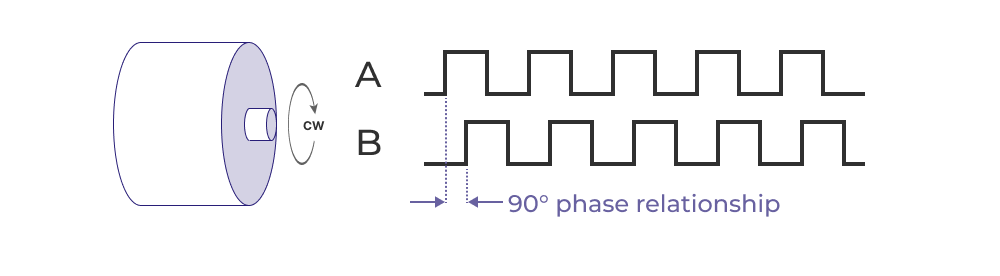
\includegraphics[width=0.85\textwidth]{fig_encoder_quadrature}
    \caption{Encoder AMT-103 และ Quadrature Signal แสดงการระบุทิศทางจากลำดับ Phase}
    \label{fig:encoder_quadrature}
\end{figure}
 
\subsubsection{Quadrature Encoding (×4)}
 
การอ่านค่าแบบ ×4 (4-edge decoding) นับทั้ง Rising Edge และ Falling Edge
ของทั้ง Channel A และ B ทำให้ Resolution เพิ่มขึ้น 4 เท่า
 
\begin{equation}
    \text{Resolution} = \text{PPR} \times 4
                      = 2048 \times 4 = 8192\;\text{counts/rev}
    \label{eq:encoder_resolution}
\end{equation}
 
ค่าตำแหน่งเชิงมุมแปลงจาก Encoder Count ได้จาก
 
\begin{equation}
    \theta\;(\text{deg}) = \frac{N_{count}}{8192} \times 360\degree
    \label{eq:encoder_to_deg}
\end{equation}
 
\noindent โดยที่ $N_{count}$ คือค่า Counter ของ TIM3 (STM32 QEI Mode)
Encoder ติดตั้งที่ Output Shaft โดยตรง (หลัง Gearbox และ Belt)
ทำให้ค่าที่อ่านได้สะท้อนตำแหน่งแขนกลจริงโดยไม่มี Backlash Error
ผ่านระบบส่งกำลัง
 
\subsubsection{Index Pulse}
 
AMT-103 มี Index Channel (Channel Z) ที่ให้พัลส์หนึ่งครั้งต่อรอบ
ใช้สำหรับยืนยันตำแหน่ง Home ระหว่าง Homing Sequence
 
% ----------------------------------------------------------------------------
\subsection{Current Sensor (WCS1800)}
\label{subsec:current_sensor_theory}
 
WCS1800 เป็น Hall-Effect Current Sensor วัดกระแสแบบ Non-contact
โดยอาศัยสนามแม่เหล็กที่เกิดจากกระแสไฟฟ้าไหลผ่านตัวนำ
แปลงเป็นแรงดันเอาต์พุตแบบ Linear
 
% -----------------------------------------------------------------------
% รูปที่ X: WCS1800 Current Sensor และ Output Characteristic
% ชื่อไฟล์แนะนำ: fig_current_sensor.pdf
% เนื้อหา: แสดงรูป WCS1800 (ซ้าย) และกราฟ V_out vs Current (ขวา)
%          พร้อม annotation จุด Zero-current voltage และ Sensitivity
% -----------------------------------------------------------------------
\begin{figure}[H]
    \centering
    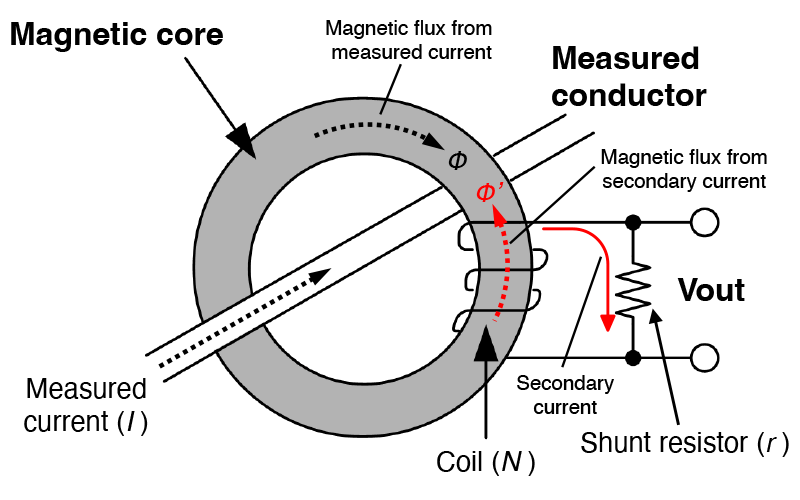
\includegraphics[width=0.80\textwidth]{fig_current_sensor}
    \caption{WCS1800 Hall-Effect Current Sensor และลักษณะการตอบสนองเชิงเส้น}
    \label{fig:current_sensor}
\end{figure}
 
\subsubsection{หลักการวัดกระแส}
 
แรงดัน Output ของ WCS1800 มีความสัมพันธ์เชิงเส้นกับกระแส
 
\begin{equation}
    V_{out} = V_{zero} + S \cdot I_a
    \label{eq:current_sensor}
\end{equation}
 
\noindent โดยที่ $V_{zero}$ คือแรงดันที่กระแสเป็นศูนย์ (ประมาณ 2.5\,V ที่ $V_{cc} = 5$\,V),
$S = 0.040$\,V/A คือ Sensitivity และ $I_a$ คือกระแสที่ต้องการวัด (A)
ค่า $V_{zero}$ ถูก Calibrate อัตโนมัติเมื่อ Boot โดยวัดเฉลี่ยจากตัวอย่าง
100 ค่าแรกในขณะที่มอเตอร์ยังไม่ทำงาน
 
\subsubsection{การนำไปใช้ใน Safety Stack}
 
ค่ากระแสที่อ่านได้ผ่านการกรองด้วย Exponential Moving Average (EMA)
เพื่อลด ADC Noise ก่อนนำไปตรวจสอบใน Safety Monitor
หากกระแสเกิน $I_{limit} = 2.0$\,A ต่อเนื่องนานกว่า 100\,ms
ระบบจะเข้าสู่ \texttt{STATE\_FAULT} (Fault Code 0x42)
 
% ----------------------------------------------------------------------------
\subsection{Proximity Sensor (Inductive)}
\label{subsec:proximity_sensor_theory}
 
Proximity Sensor แบบ Inductive ตรวจจับวัตถุโลหะโดยไม่สัมผัส
โดยอาศัยการเปลี่ยนแปลงของสนามแม่เหล็กไฟฟ้าเมื่อมีวัตถุเข้ามาในระยะตรวจจับ
ใช้สำหรับระบุตำแหน่ง Home ใน Two-Stage Homing Sequence
 
% -----------------------------------------------------------------------
% รูปที่ X: Proximity Sensor และการติดตั้งบนแขนกล
% ชื่อไฟล์แนะนำ: fig_proximity_sensor.pdf
% เนื้อหา: แสดงรูป Sensor ที่ติดตั้ง (ซ้าย) และ Timing Diagram ของสัญญาณ
%          ระหว่าง Homing: Edge A, Backoff, Edge B, Center (ขวา)
% -----------------------------------------------------------------------
\begin{figure}[H]
    \centering
    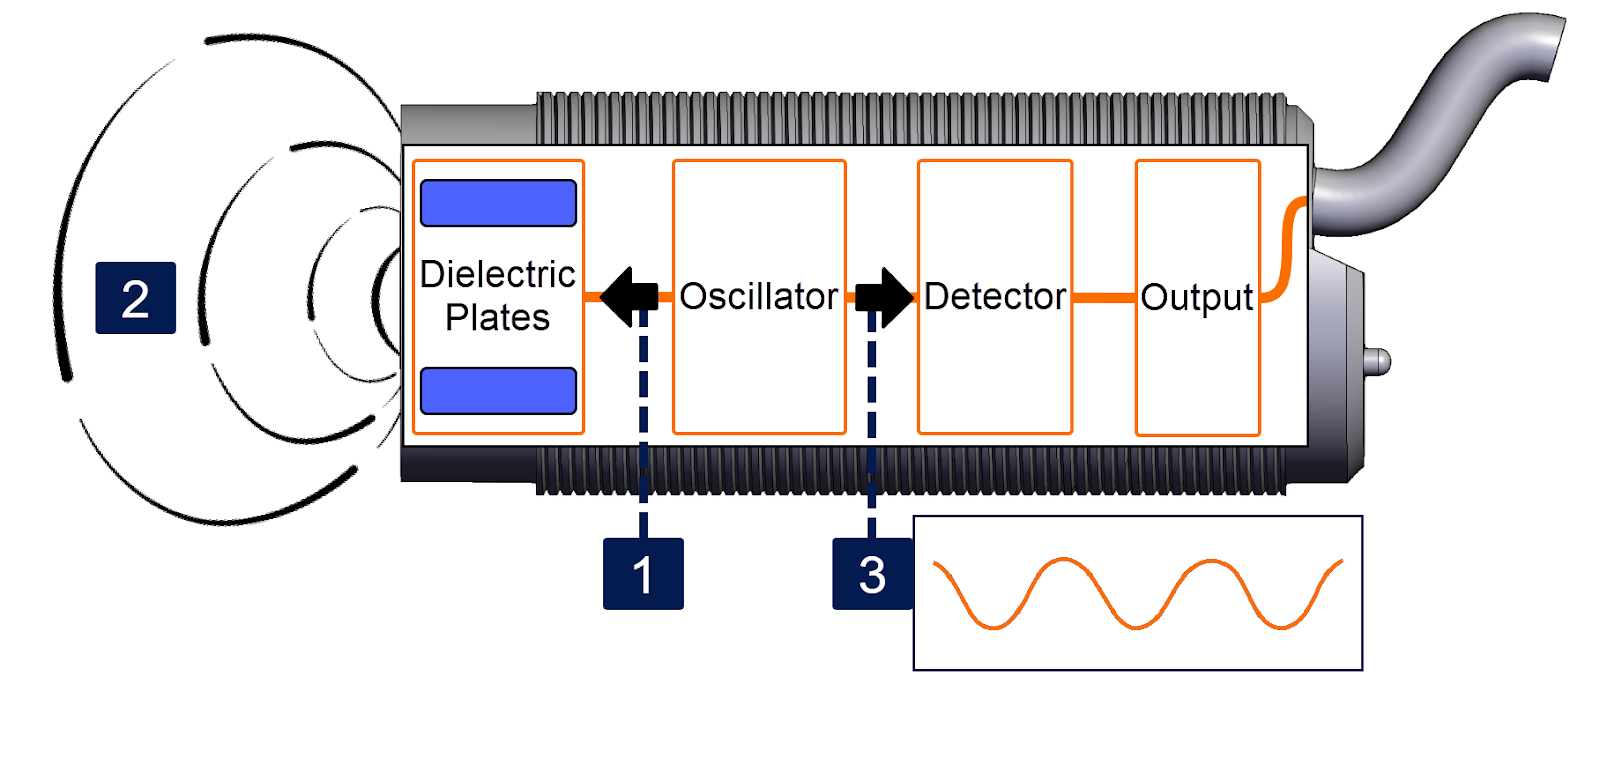
\includegraphics[width=0.85\textwidth]{fig_proximity_sensor}
    \caption{Proximity Sensor บนแขนกลและ Timing Diagram ของสัญญาณระหว่าง Two-Stage Homing}
    \label{fig:proximity_sensor}
\end{figure}
 
\subsubsection{วงจรเอาต์พุตแบบ Open-Collector}
 
Sensor ที่ใช้เป็นแบบ Open-Collector Optocoupler
โดยมีสถานะดังนี้
 
\begin{itemize}
    \item \textbf{ไม่มีวัตถุ (Normal):} Transistor นำกระแส ขา Output ถูก Pull ลง GND \texttt{LOW}
    \item \textbf{มีวัตถุ (Triggered):} Transistor หยุดนำกระแส ขา Output ลอย
          ถูก Pull-up ขึ้น 3.3\,V ผ่าน Internal PULLUP ของ STM32 \texttt{HIGH}
\end{itemize}
 
ดังนั้น Active Condition คือ \texttt{GPIO\_PIN\_SET} (HIGH)
และต้องตั้งค่า GPIO เป็น \texttt{GPIO\_PULLUP} เสมอ
การตั้งค่าเป็น \texttt{GPIO\_PULLDOWN} จะทำให้ทั้งสองสถานะเป็น 0\,V
และ MCU ไม่สามารถตรวจจับสัญญาณได้
 
\subsubsection{การนำไปใช้ใน Homing Sequence}
 
Proximity Sensor ใช้ Debounce 1 tick (10\,ms) ซึ่งสั้นกว่า Sensor อื่น
เนื่องจาก Detection Zone แคบ ต้องการการตอบสนองที่รวดเร็วเพื่อจับ Edge ได้แม่นยำ
ระบบ Homing ใช้หลักการ Midpoint Capture ระหว่าง Edge A และ Edge B
ซึ่งมาจากทิศทางตรงกันข้ามที่ความเร็วเท่ากัน
ทำให้ค่ากึ่งกลางที่ได้ไม่มี Bias จาก Sensor Switching Delay
% ============================================================================
%  บทที่ 3: สถาปัตยกรรมและการออกแบบระบบ
% ============================================================================

\chapter{สถาปัตยกรรมและการออกแบบระบบ}
\label{ch:design}

% ============================================================================
\section{สถาปัตยกรรมระบบภาพรวม}
\label{sec:system_arch}
% ============================================================================

ระบบ Circular Pick and Place Robot ออกแบบตามหลัก Cyber-Physical System
โดยแบ่งสถาปัตยกรรมออกเป็น Physical Layer ซึ่งประกอบด้วยฮาร์ดแวร์จริง
และ Cyber Layer ซึ่งประกอบด้วยโครงสร้าง Firmware และ Communication
ภายใน STM32G474RE ดังแสดงใน\cref{fig:sys_arch}

% -----------------------------------------------------------------------
% รูปที่: System Architecture Overview
% ชื่อไฟล์แนะนำ: fig_system_architecture.png
% เนื้อหา: Layered block diagram แสดง 4 ระดับ (External $\rightarrow$ STM32 Cyber $\rightarrow$
%          Power Management $\rightarrow$ Physical Actuators/Sensors)
%          พร้อม color coding: blue=signal, red=power, green=mechanical
% -----------------------------------------------------------------------
\begin{figure}[H]
    \centering
    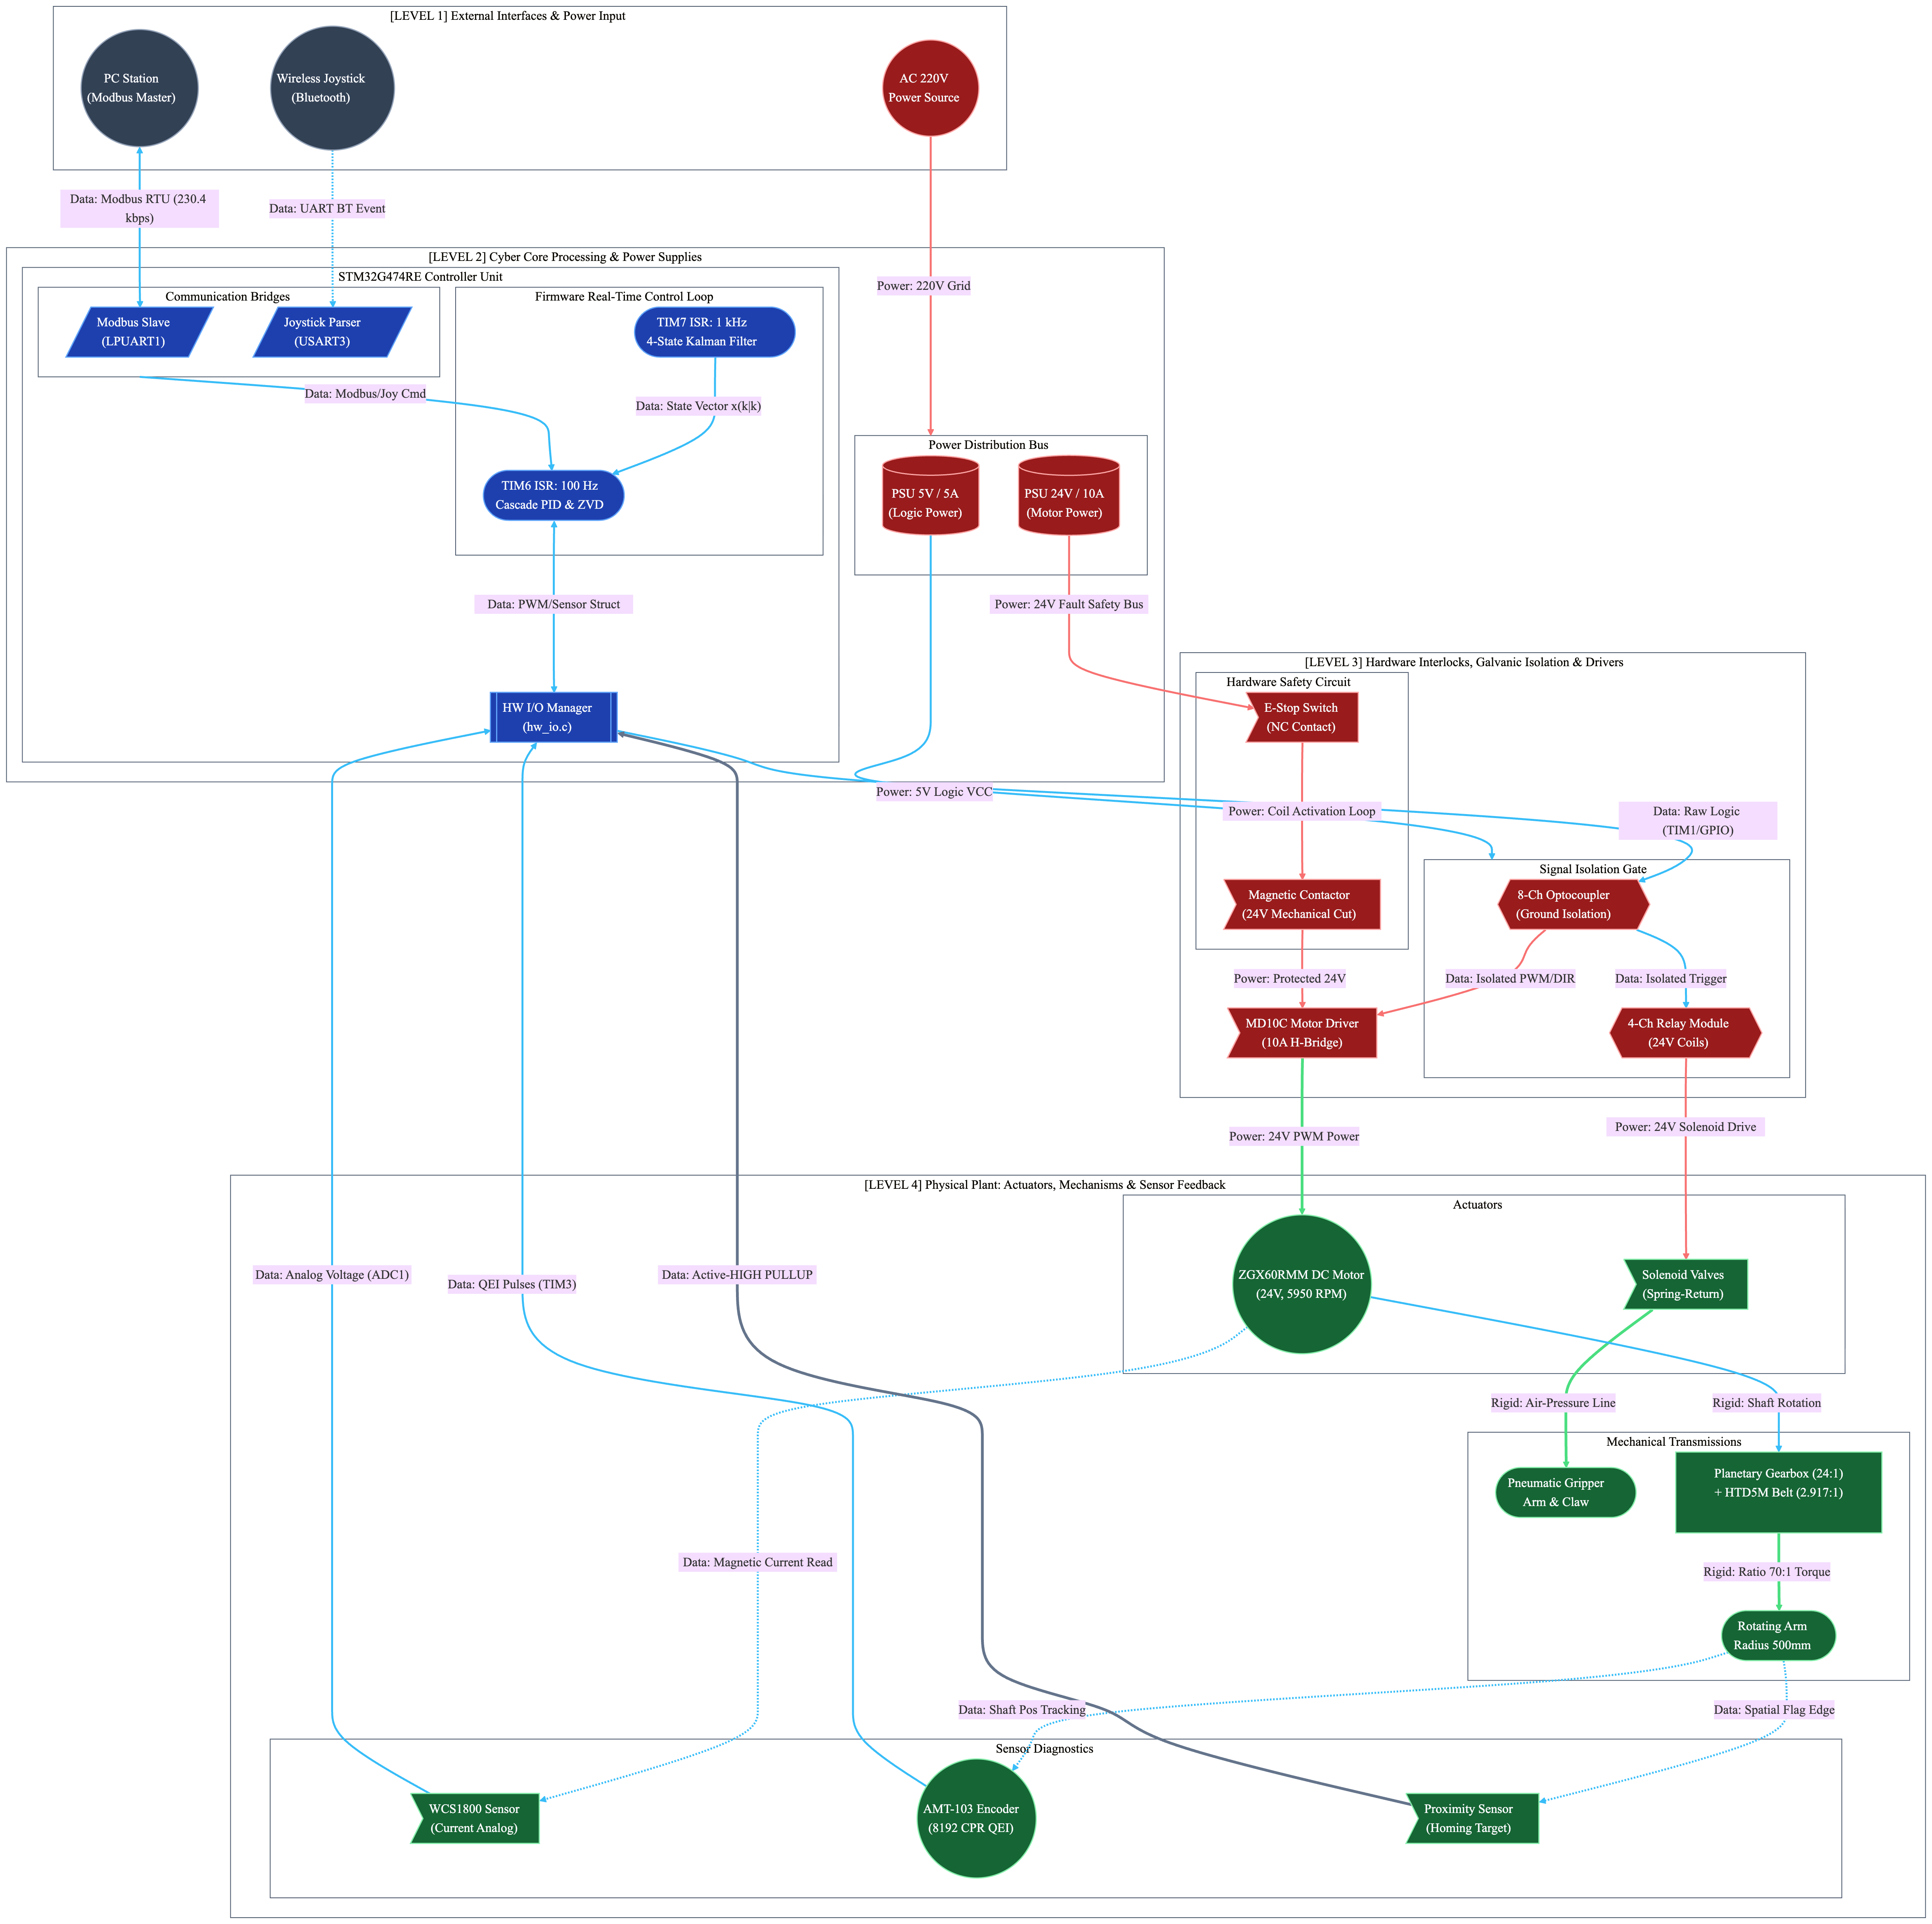
\includegraphics[width=0.95\textwidth]{fig_system_architecture}
    \caption{System Architecture ของระบบ Circular Pick and Place Robot
             แสดง Physical Architecture และ Cyber Architecture}
    \label{fig:sys_arch}
\end{figure}

% -----------------------------------------------------------------------
\subsection{ห่วงโซ่การส่งกำลัง (Power Transmission Chain)}
\label{subsec:drivetrain_arch}
% -----------------------------------------------------------------------

ข้อกำหนด P3 กำหนดให้ความเร็วเชิงมุมที่เพลาแขนกลอยู่ในช่วง
$2.9 \leq \omega \leq 5.84$\,rad/s และ P4 กำหนดให้ความเร่งสูงสุด
$\alpha_{max} \leq 22.0$\,rad/s$^2$ ในขณะที่มอเตอร์ RS-775 มีความเร็วสูงสุด
5,950\,RPM ($\approx 623$\,rad/s) แสดงว่าระบบต้องการอัตราทดรวม
ในช่วง $N \approx 70$ เพื่อแปลงความเร็วสูงของมอเตอร์ให้เป็น
แรงบิดสูงสำหรับงานหยิบวางชิ้นงาน 2\,kg ที่รัศมี 500\,mm

การบรรลุอัตราทดดังกล่าวด้วย Single-stage Gearbox เพียงอย่างเดียว
จะทำให้ขนาดของ Gearbox ใหญ่เกินขีดจำกัดฐาน 200$\times$200\,mm
(ข้อกำหนด M1) ระบบจึงออกแบบเป็น 2-stage โดยแยกหน้าที่ดังนี้

\begin{itemize}
  \item \textbf{Planetary Gearbox} ($N_g = 24$): รับภาระ Torque Amplification
        หลัก เนื่องจาก Planetary configuration ให้อัตราทดสูงในขนาด
        Footprint เล็กกว่า Spur Gear ที่อัตราทดเทียบเท่า
  \item \textbf{Belt Drive HTD5M} ($N_b = 70/24 \approx 2.917$):
        ทำหน้าที่ปรับ Layout โดยส่งกำลังข้ามระยะ Center Distance 181.25\,mm
        เพื่อแยกตำแหน่งมอเตอร์ออกจากจุดหมุนของแขนกล
        ซึ่งช่วยลดโมเมนต์ความเฉื่อยของส่วนที่หมุน
        และยังทำให้สามารถติดตั้ง Encoder ได้โดยตรง
        ที่ Output Shaft โดยไม่ผ่าน Gearbox
\end{itemize}

อัตราทดรวม $N = N_g \times N_b = 24 \times 2.917 = 70$ และ
ประสิทธิภาพรวม $\eta = \eta_{gear} \times \eta_{belt} = 0.88 \times 0.95 = 0.836$
ให้แรงบิดที่เพลาแขนกล

\begin{equation}
  T_{arm} = T_{motor} \times N \times \eta
           = 0.0955 \times 70 \times 0.836
           = 5.40\,\text{N}\cdot\text{m}
  \label{eq:tarm_verify}
\end{equation}

ซึ่งมี Safety Factor เทียบกับแรงบิดที่ต้องการ
$T_{req} = J \cdot \alpha_{min} \times SF = 0.5764 \times 2.0 \times 2.0 = 2.31$\,N$\cdot$m
คือ $SF_{actual} = 5.40 / 2.31 = 2.34 > 2.0$ \textbf{(ผ่าน P3, P4)}

\textbf{การติดตั้ง Encoder ที่ Output Shaft:}
เพื่อลด Backlash Error ที่สะสมจากทั้ง Planetary Gearbox และ Belt Drive
Encoder AMT-103 จึงติดตั้งโดยตรงที่ Output Shaft ซึ่งเป็นตำแหน่ง
\emph{หลัง} ระบบส่งกำลังทั้งหมด Control Loop จึงปิดผ่านตำแหน่ง
จริงของแขนกลโดยตรง ทำให้ Backlash ในทุก Stage
ไม่ส่งผลต่อ Closed-loop Accuracy และ Repeatability (A2)

% -----------------------------------------------------------------------
% รูปที่: แผนผังห่วงโซ่การส่งกำลัง
% ชื่อไฟล์แนะนำ: fig_drivetrain_chain.png
% เนื้อหา: Block diagram ลำดับ Motor $\rightarrow$ Planetary Gearbox $\rightarrow$ Belt $\rightarrow$ Output Shaft
%          แสดงค่า RPM, Torque, และ N ที่แต่ละจุด พร้อมตำแหน่ง Encoder
% -----------------------------------------------------------------------
\begin{figure}[H]
    \centering
    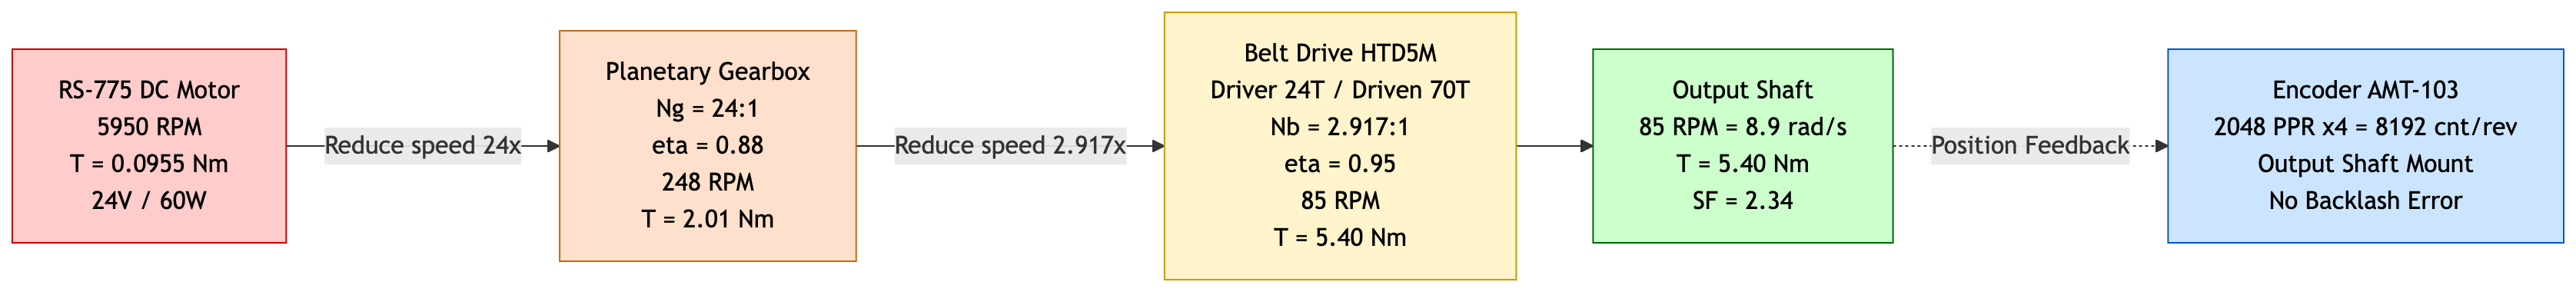
\includegraphics[width=\textwidth]{fig_drivetrain_chain}
    \caption{แผนผังห่วงโซ่การส่งกำลังแสดงการเปลี่ยนแปลงความเร็วและแรงบิด
             ตั้งแต่มอเตอร์ถึงแขนกล พร้อมตำแหน่ง Encoder ที่ Output Shaft}
    \label{fig:drivetrain_chain}
\end{figure}

% -----------------------------------------------------------------------
\subsection{Application Finite State Machine}
\label{subsec:fsm_arch}
% -----------------------------------------------------------------------

โครงสร้าง FSM ออกแบบให้ตอบสนองข้อกำหนดด้านความปลอดภัยและการใช้งาน
พร้อมกันในเวลาเดียว ระบบมี 5 สถานะหลักดังนี้

\begin{itemize}
  \item \textbf{\texttt{INIT}:} ตรวจสอบฮาร์ดแวร์และโหลดค่า Configuration
        จาก Flash ก่อนอนุญาตให้ระบบทำงาน
  \item \textbf{\texttt{HOMING}:} ค้นหาจุด Home ด้วย Two-Stage Homing
        (Coarse Search ไป Fine Search ด้วย Proximity Sensor)
        ตามข้อกำหนด A3 ที่ต้องสามารถตั้งจุด Home ได้หลังติดตั้ง
  \item \textbf{\texttt{IDLE}:} พร้อมรับคำสั่ง รอ Command จาก Modbus
        หรือ Joystick โดยตรวจสอบ Heartbeat Watchdog ต่อเนื่อง
  \item \textbf{\texttt{RUNNING}:} กำลังประมวลผล Motion Sequence
        ทั้ง Pick-Place Cycle และ Manual Jog
  \item \textbf{\texttt{FAULT}:} หยุดฉุกเฉิน ตัด PWM ทันที
        และ Log Fault Code เพื่อ Diagnosis
\end{itemize}

ทุกสถานะสามารถเข้าสู่ \texttt{FAULT} ได้จาก E-Stop Hardware หรือ
Software Safety Fault (Overcurrent, Heartbeat Timeout, Workspace Violation)
โดยไม่ผ่านสถานะกลาง เพื่อรับประกัน Worst-case Response Time
ที่ขึ้นกับ TIM6 ISR Period ($\leq 1$\,ms) เท่านั้น

สถานะ \texttt{FAULT} ตัดเฉพาะ PWM Output (Motor Power)
แต่ STM32 ยังคงรัน Firmware ต่อเนื่องเพื่อรับ Reset Command
และรายงาน Fault Code ผ่าน Modbus ซึ่งเป็นไปตามข้อกำหนด E6
ที่กำหนดให้ Controller มีไฟเลี้ยงแม้หลังกด E-Stop
สอดคล้องกับการออกแบบ Power Bus แบบ Dual-rail ใน\cref{subsec:elec_arch}

% -----------------------------------------------------------------------
% รูปที่: FSM State Diagram
% ชื่อไฟล์แนะนำ: fig_fsm_diagram.png
% เนื้อหา: State diagram แสดง 5 states (INIT, HOMING, IDLE, RUNNING, FAULT)
%          พร้อม transition conditions และ entry/exit actions
%          เน้น FAULT transitions จากทุก state ด้วยลูกศรสีแดง
% -----------------------------------------------------------------------
\begin{figure}[H]
    \centering
    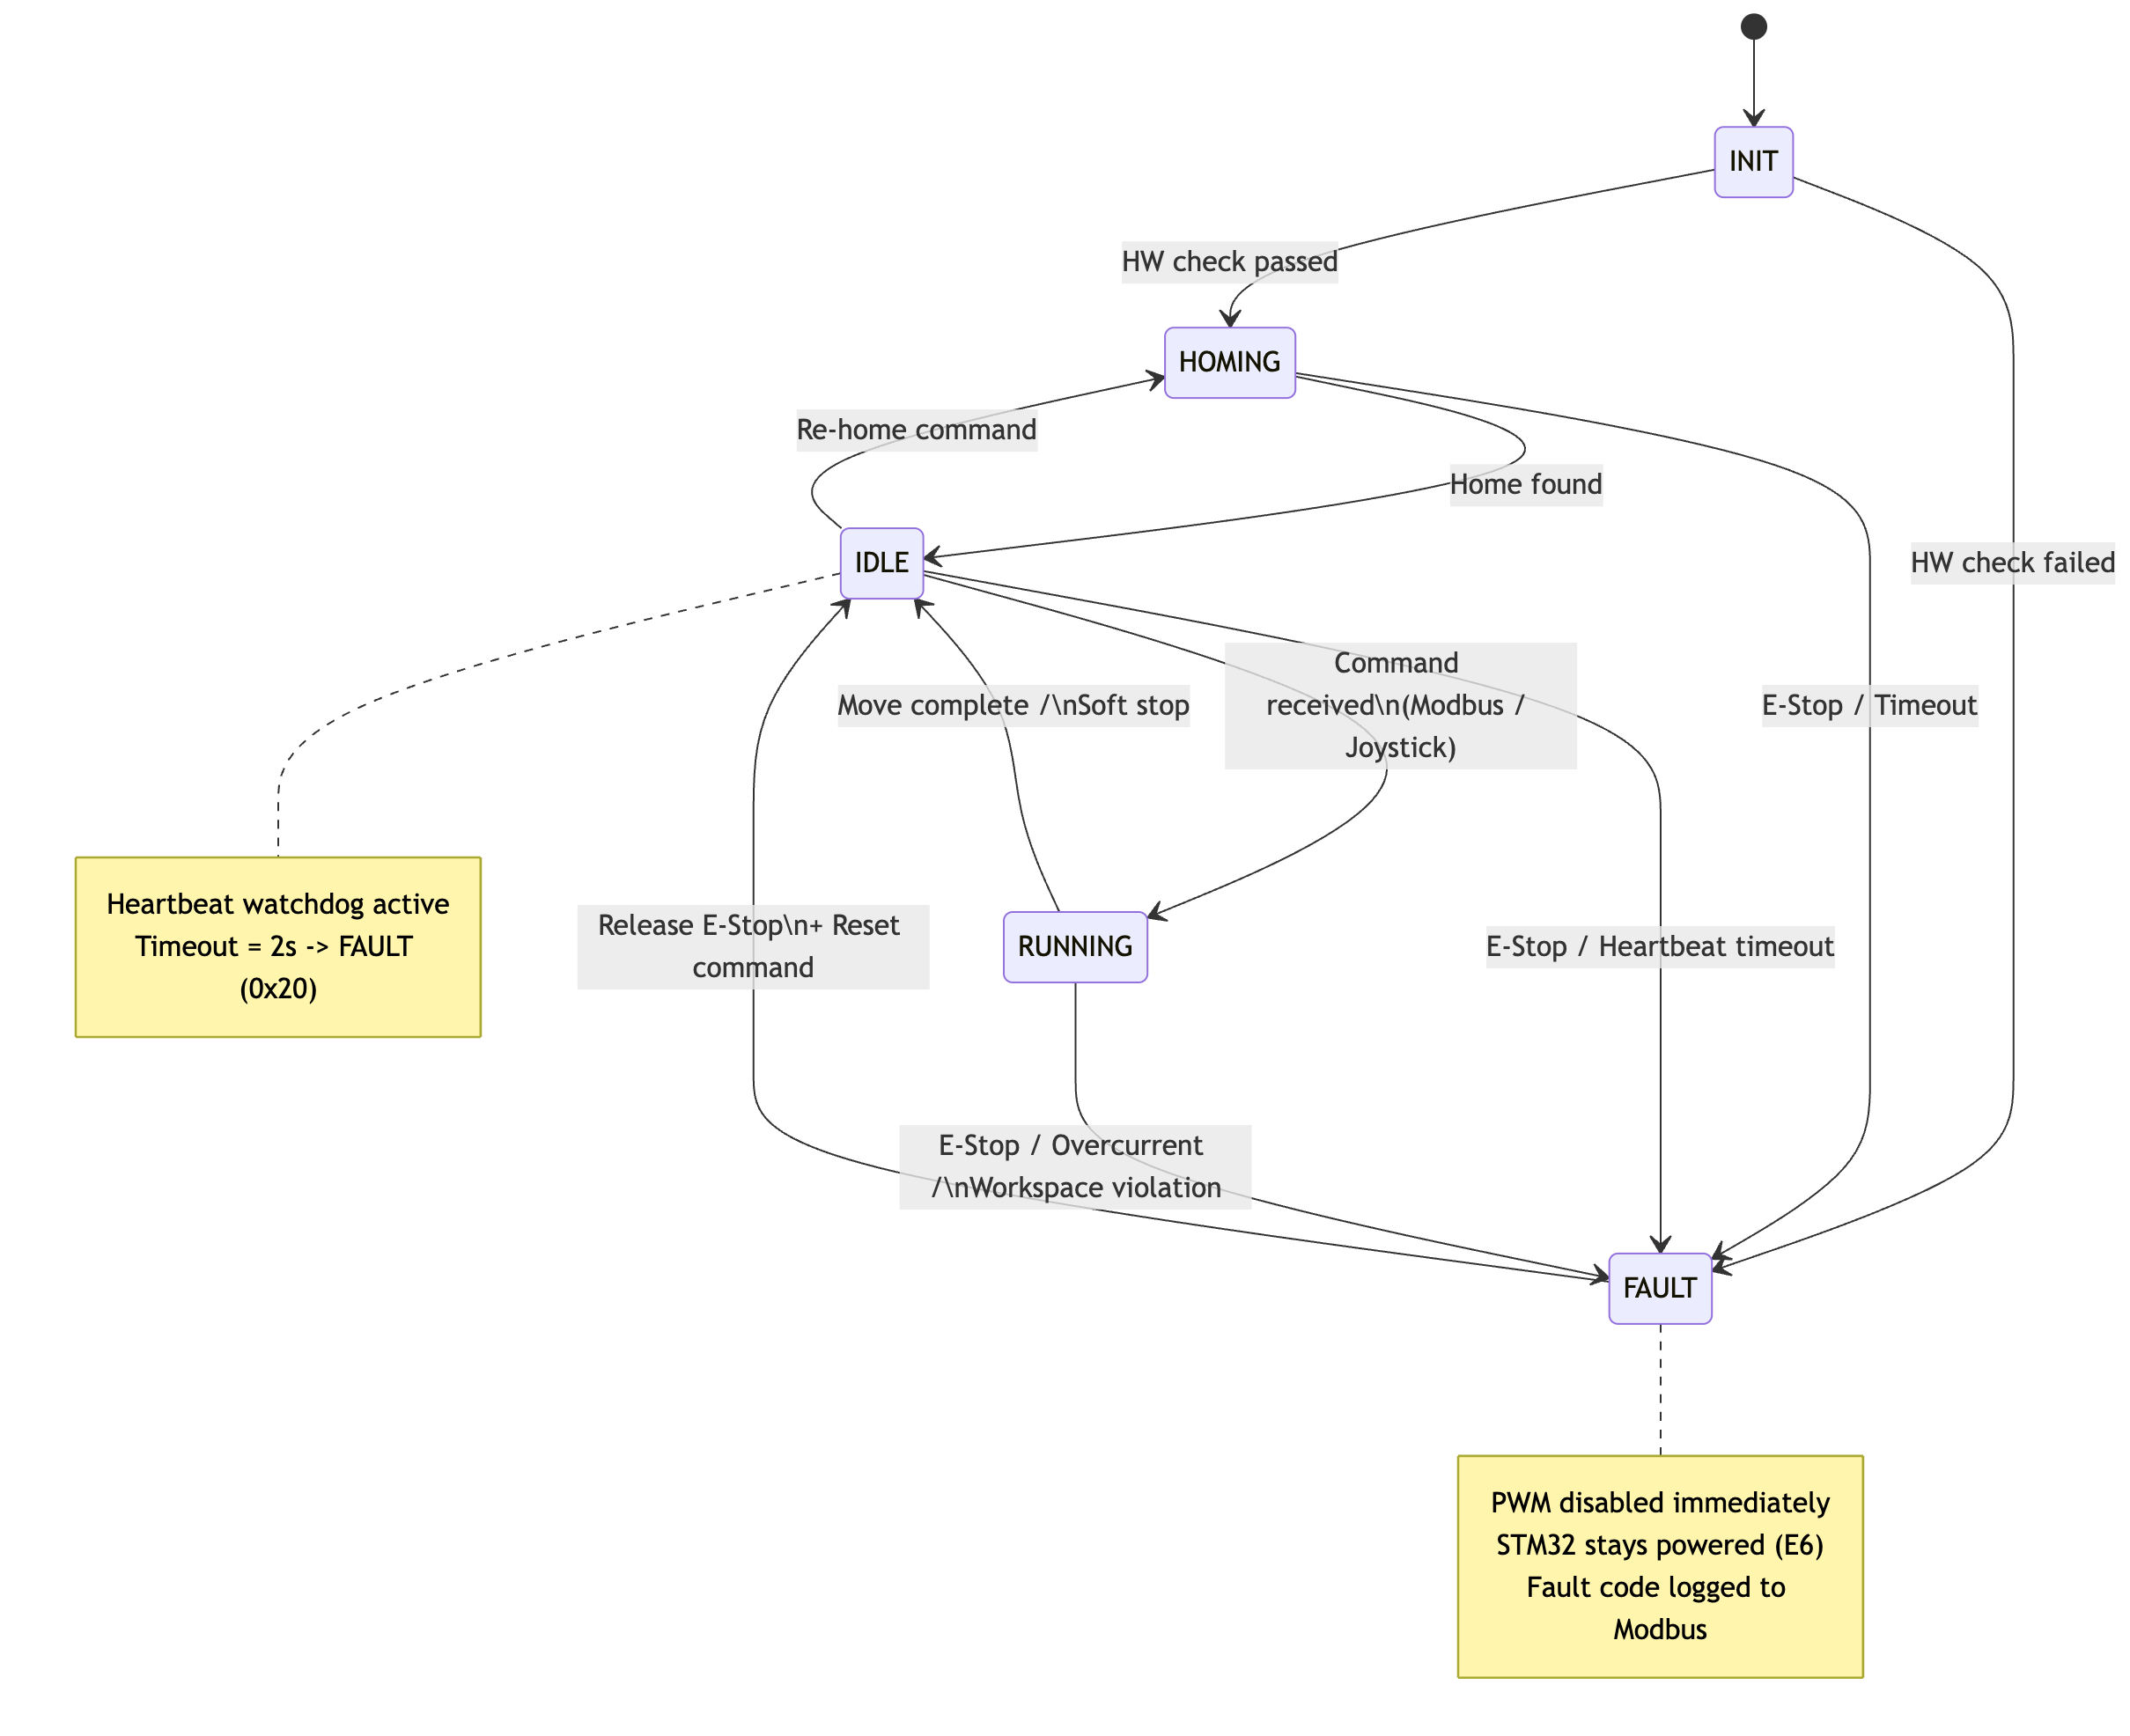
\includegraphics[width=0.80\textwidth]{fig_fsm_diagram}
    \caption{Application FSM แสดง 5 สถานะหลักและเงื่อนไข Transition
             โดย FAULT สามารถถูก Trigger ได้จากทุกสถานะ (ลูกศรสีแดง)}
    \label{fig:fsm_diagram}
\end{figure}

% ============================================================================
\section{การออกแบบเชิงกล}
\label{sec:mech_design}
% ============================================================================

\subsection{สถาปัตยกรรมเชิงกลโดยรวม}
\label{subsec:mech_arch}

โครงสร้างเชิงกลของระบบแบ่งออกเป็น 3 ส่วนหลักที่ประกอบกัน ได้แก่
ส่วนฐาน (Base) ที่ยึดกับแท่นของลูกค้าด้วยสกรู M8 ตามข้อกำหนด M7,
ส่วนแขนกล (Rotating Arm) รัศมี 500\,mm ที่หมุนรอบแกนแนวตั้ง
และชุดส่งกำลัง 2-stage ที่อธิบายใน\cref{subsec:drivetrain_arch}
ภาพรวม CAD Assembly แสดงใน\cref{fig:mech_cad}

% -----------------------------------------------------------------------
% รูปที่: CAD Assembly ภาพรวม
% ชื่อไฟล์แนะนำ: fig_cad_assembly.png
% เนื้อหา: CAD render มุมมอง Isometric แสดง Base, Arm, Gearbox,
%          Belt Drive, Encoder mount และ Gripper Housing
%          ควร label ส่วนประกอบหลักด้วย callout
% -----------------------------------------------------------------------
\begin{figure}[H]
    \centering
    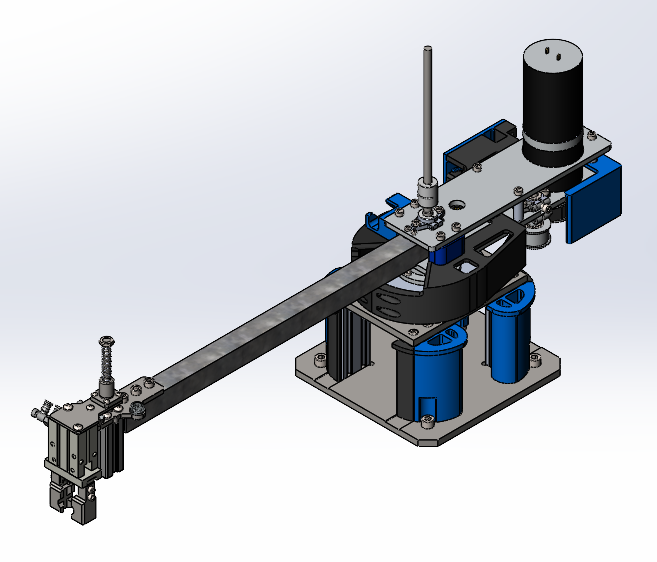
\includegraphics[width=0.75\textwidth]{fig_cad_assembly}
    \caption{CAD Assembly ของระบบเชิงกล แสดงส่วนประกอบหลักทั้งหมด}
    \label{fig:mech_cad}
\end{figure}

% -----------------------------------------------------------------------
\subsection{การคำนวณเพลา}
\label{subsec:shaft_calc}
% -----------------------------------------------------------------------

การคำนวณขนาดเพลาดำเนินการตาม Maximum Shear Stress Theory (ASME Code)
โดยมีจุดวิกฤตอยู่ที่ตำแหน่งลูกปืนบน ซึ่งรับทั้งโมเมนต์ดัดจากน้ำหนัก
ปลายแขนและแรงดึงสายพานพร้อมกัน

\subsubsection{พารามิเตอร์และวัสดุ}

\begin{table}[H]
  \centering
  \caption{พารามิเตอร์ภาระโหลดของระบบเพลา}
  \label{tab:shaft_loads}
  \begin{tabular}{llll}
    \toprule
    พารามิเตอร์ & สัญลักษณ์ & ค่า & หน่วย \\
    \midrule
    มวลโหลดที่ปลายเพลา        & $m$        & 3.72   & kg \\
    น้ำหนักโหลดในแนวดิ่ง       & $W$        & 37.20  & N \\
    ระยะเยื้องศูนย์            & $L_{cg}$   & 46.63  & mm \\
    ความเร็วรอบ               & $n$        & 85.00  & RPM \\
    แรงเหวี่ยงหนีศูนย์กลาง     & $F_c$      & 13.75  & N \\
    แรงดึงสายพานรวม            & $F_{belt}$ & 130.00 & N \\
    ระยะจากโหลดถึงลูกปืนบน    & $L_1$      & 25.25  & mm \\
    ระยะลูกปืนบนถึงล่าง        & $L_2$      & 37.25  & mm \\
    \bottomrule
  \end{tabular}
\end{table}

วัสดุเพลาเลือกใช้ Stainless Steel AISI~304
เนื่องจากเป็นวัสดุมาตรฐานที่หาซื้อได้ง่ายในตลาดไทย
มี Yield Strength $S_{yt} = 215$\,MPa
เพียงพอสำหรับการรับภาระในระบบนี้
และ Allowable Shear Stress ตามมาตรฐาน ASME คือ

\begin{equation}
  \tau_{allow} = 0.30 \times S_{yt} = 0.30 \times 215 = 64.5\,\text{MPa}
  \label{eq:shaft_tau_allow}
\end{equation}

% -----------------------------------------------------------------------
% รูปที่: Free Body Diagram เพลา
% ชื่อไฟล์แนะนำ: fig_shaft_fbd.png
% เนื้อหา: FBD แสดง W, Fc, Fbelt ที่กระทำต่อเพลา
%          พร้อม reaction forces ที่ลูกปืนบนและล่าง
%          และระบุจุดวิกฤตด้วยลูกศรหรือ highlight
% -----------------------------------------------------------------------
\begin{figure}[H]
    \centering
    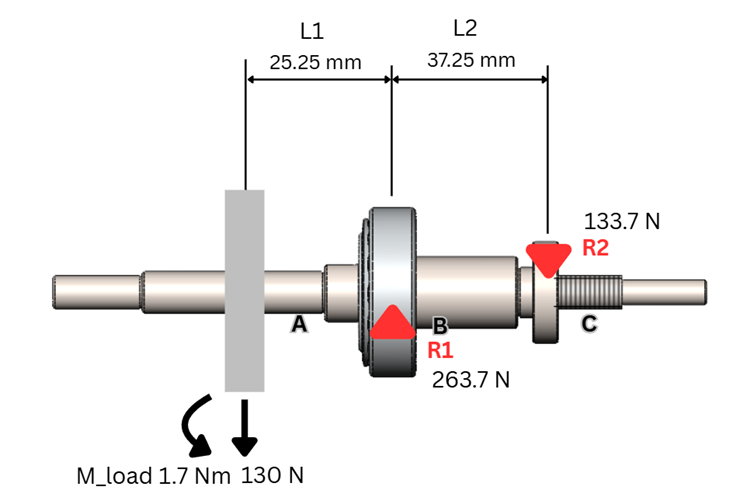
\includegraphics[width=0.75\textwidth]{fig_shaft_fbd}
    \caption{Free Body Diagram ของระบบเพลาแสดงแรงและโมเมนต์ที่จุดวิกฤต}
    \label{fig:shaft_fbd}
\end{figure}

\subsubsection{การวิเคราะห์โมเมนต์ดัด}

โมเมนต์ดัดจากโหลดปลายแขนและแรงเหวี่ยง

\begin{equation}
  M_{overhang} = (W + F_c) \times L_1
               = (37.20 + 13.75) \times 0.02525
               = 1.287\,\text{N}\cdot\text{m}
  \label{eq:shaft_m_overhang}
\end{equation}

โมเมนต์ดัดจากแรงดึงสายพาน

\begin{equation}
  M_{belt} = F_{belt} \times L_1
           = 130.00 \times 0.02525
           = 3.283\,\text{N}\cdot\text{m}
  \label{eq:shaft_m_belt}
\end{equation}

โมเมนต์รวม Worst-case โดย Vector Superposition (ทิศทางเสริมกัน)

\begin{equation}
  M_{total} = 5.014\,\text{N}\cdot\text{m}
  \label{eq:shaft_m_total}
\end{equation}

\subsubsection{การคำนวณขนาดเพลา}

เลือก Fatigue Shock Factors $C_m = 2.0$ (Bending) และ $C_t = 1.5$ (Torsion)
สำหรับสภาวะ Light Shock เนื่องจาก S-curve Trajectory จำกัด Jerk
ให้ไม่เกิน $j_{max} = 1400$\,rad/s$^3$ ทำให้ภาระที่เพลา
เปลี่ยนแปลงแบบต่อเนื่องไม่ใช่ Impact Load
แต่ยังคง $C_m > 1$ เพื่อรองรับ Transient ที่อาจเกิดขณะ
Emergency Stop

\begin{equation}
  d_{min} = \left[
    \frac{16}{\pi\,\tau_{allow}}
    \sqrt{(C_m M_{total})^2 + (C_t T)^2}
  \right]^{1/3}
  \label{eq:shaft_dmin}
\end{equation}

\begin{equation}
  d_{min} = \left[
    \frac{16}{\pi \times 64.5 \times 10^6}
    \sqrt{(2.0 \times 5.014)^2 + (1.5 \times 5.398)^2}
  \right]^{1/3}
  = 10.59\,\text{mm}
  \label{eq:shaft_result}
\end{equation}

\subsubsection{การออกแบบ Step Shaft}

แม้ว่า $d_{min} = 10.59$\,mm จากการวิเคราะห์ความล้า
แต่ขนาดจริงที่จุดวิกฤตถูกกำหนดโดย Bearing Seat ของ
SKF~30203 Tapered Roller Bearing ซึ่งมี ID~=~17\,mm
ดังนั้นจึงเลือก $d_{actual} = 17$\,mm ที่จุดวิกฤต
ซึ่งให้ FOS~$\geq 1.6$ เทียบกับ $d_{min}$

เพลาออกแบบเป็น Step Shaft เพื่อรองรับ Bearing
ที่ขนาดต่างกัน และสร้าง Shoulder สำหรับ Axial Location
ดังสรุปใน\cref{tab:shaft_summary}

\begin{table}[H]
  \centering
  \caption{สรุปผลการคำนวณเพลาและการออกแบบ Step Shaft}
  \label{tab:shaft_summary}
  \begin{tabular}{lccl}
    \toprule
    พารามิเตอร์ & ค่า & หน่วย & หมายเหตุ \\
    \midrule
    $M_{total}$ (Worst-case)  & 5.014 & N$\cdot$m & Vector Superposition \\
    $T$ (Torsion)             & 5.398 & N$\cdot$m & จากระบบส่งกำลัง \\
    $d_{min}$ (คำนวณ)         & 10.59 & mm        & จุดวิกฤต (Fatigue) \\
    $d_{actual}$ (จุดวิกฤต)   & 17    & mm        & Bearing Seat SKF 30203 \\
    $d$ (ช่วงกลาง)            & 12    & mm        & ผ่าน \\
    $d$ (ช่วงปลาย)            & 8--10 & mm        & ไม่ใช่จุดวิกฤต \\
    \bottomrule
  \end{tabular}
\end{table}

% -----------------------------------------------------------------------
\subsection{การวิเคราะห์เพลาด้วย FEA (Shaft FEA)}
\label{subsec:shaft_fea}
% -----------------------------------------------------------------------

เพื่อยืนยันผลการคำนวณเชิงวิเคราะห์ใน\cref{subsec:shaft_calc}
ดำเนินการวิเคราะห์ Finite Element Analysis (Static Study)
ด้วย SOLIDWORKS Simulation โดยจำลองเพลาเป็น Beam Element
ซึ่งเหมาะสมกับโครงสร้างที่มี Aspect Ratio สูง (ความยาวรวม $\approx 68$\,mm
เทียบกับเส้นผ่าศูนย์กลางสูงสุด 17\,mm)
การใช้ Beam Mesh แทน Solid Mesh ในกรณีนี้ให้ความแม่นยำเทียบเท่า
แต่ใช้ Computational Cost ต่ำกว่าอย่างมีนัยสำคัญ
เนื่องจากทฤษฎี Euler–Bernoulli Beam ถูกต้องเมื่อ
$L/d > 10$ ซึ่งเป็นเงื่อนไขที่เพลานี้ตอบสนองได้

\subsubsection{สภาวะการจำลอง (FEA Setup)}

โมเดลเพลาแบบ Step Shaft สร้างขึ้นใน SOLIDWORKS โดยแบ่งออกเป็น
6 Beam Segment ตามขนาดเส้นผ่าศูนย์กลางที่เปลี่ยนไปในแต่ละช่วง
วัสดุที่ใช้คือ Stainless Steel AISI~304 ซึ่งสอดคล้องกับการออกแบบ
ใน\cref{subsec:shaft_calc}

\begin{table}[H]
  \centering
  \caption{คุณสมบัติวัสดุที่ใช้ใน FEA เพลา (AISI 304)}
  \label{tab:shaft_fea_material}
  \begin{tabular}{lll}
    \toprule
    คุณสมบัติ & ค่า & หน่วย \\
    \midrule
    Yield Strength   & $2.068 \times 10^8$ & N/m$^2$ \\
    Tensile Strength & $5.170 \times 10^8$ & N/m$^2$ \\
    Elastic Modulus  & $1.900 \times 10^{11}$ & N/m$^2$ \\
    Poisson's Ratio  & 0.29 & -- \\
    Mass Density     & 8,000 & kg/m$^3$ \\
    Shear Modulus    & $7.500 \times 10^{10}$ & N/m$^2$ \\
    \bottomrule
  \end{tabular}
\end{table}

กำหนด Boundary Conditions ดังนี้

\begin{itemize}
  \item \textbf{Fixture:} Immovable (No Translation) ที่ Joint
        ตำแหน่งลูกปืนบน (SKF~30203) และลูกปืนล่าง (F6901ZZ)
        จำลองการยึดแน่นของ Bearing Housing ในแนวรัศมี
  \item \textbf{Load:} แรงดึงสายพาน $F_{belt} = 130$\,N
        ในแนวรัศมีที่ตำแหน่ง Belt Pulley
        และ Moment $M = 1.7$\,N$\cdot$m
        (แรงบิดที่ส่งผ่านสายพานเมื่อระบบทำงานเต็มกำลัง)
  \item \textbf{Mesh:} Beam Mesh, 37 Nodes, 30 Elements
        (Automatic, High Quality)
\end{itemize}

% -----------------------------------------------------------------------
% รูปที่: Shaft FEA — Load and Fixture Setup
% ชื่อไฟล์แนะนำ: fig_shaft_fea_setup.png
% เนื้อหา: SOLIDWORKS screenshot แสดง Step Shaft พร้อม
%          Fixture ที่ตำแหน่งลูกปืน (สีฟ้า) และ
%          แรง F=130N + Moment=1.7N.m ที่ตำแหน่ง Pulley (ลูกศรสีชมพู)
% -----------------------------------------------------------------------
\begin{figure}[H]
    \centering
    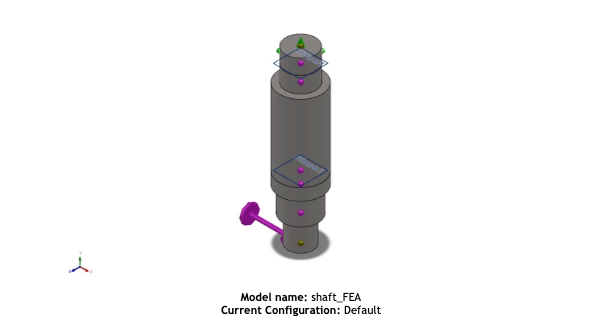
\includegraphics[width=0.75\textwidth]{fig_shaft_fea_setup}
    \caption{การตั้งค่าโมเดล FEA เพลา แสดง Fixture ที่ตำแหน่งลูกปืน
             และภาระแรงดึงสายพาน 130\,N พร้อม Moment 1.7\,N$\cdot$m}
    \label{fig:shaft_fea_setup}
\end{figure}

\subsubsection{ผลการวิเคราะห์ FEA เพลา}

% -----------------------------------------------------------------------
% รูปที่: Shaft FEA — Stress Distribution
% ชื่อไฟล์แนะนำ: fig_shaft_fea_stress.png
% เนื้อหา: SOLIDWORKS color map (Upper bound axial and bending stress)
%          Max = 2.221e+07 N/m² ที่ Element 24 (บริเวณ Belt Pulley seat)
%          แสดง deformed shape + color scale
% -----------------------------------------------------------------------
\begin{figure}[H]
    \centering
    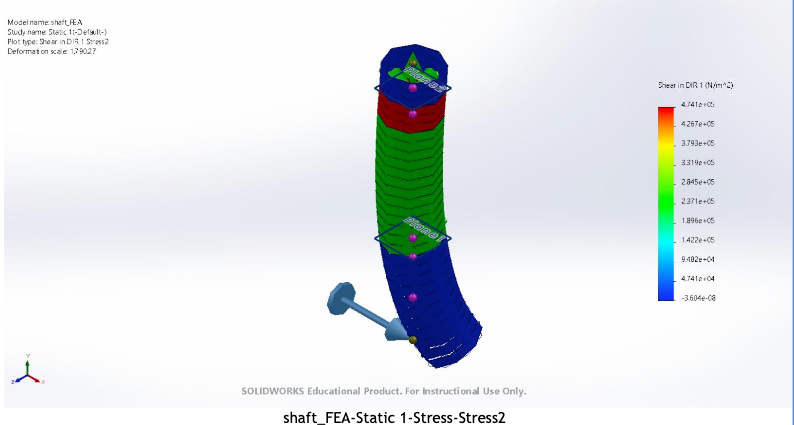
\includegraphics[width=0.75\textwidth]{fig_shaft_fea_stress}
    \caption{ผล FEA เพลา: การกระจายตัวของ Upper Bound Axial and Bending Stress
             (Max $= 2.221 \times 10^7$\,N/m$^2$ บริเวณตำแหน่ง Belt Pulley)}
    \label{fig:shaft_fea_stress}
\end{figure}

% -----------------------------------------------------------------------
% รูปที่: Shaft FEA — Displacement
% ชื่อไฟล์แนะนำ: fig_shaft_fea_displacement.png
% เนื้อหา: SOLIDWORKS color map ของ URES Resultant Displacement
%          Max = 4.721e-03 mm ที่ Node 30 (ปลายเพลาด้านล่าง)
% -----------------------------------------------------------------------
\begin{figure}[H]
    \centering
    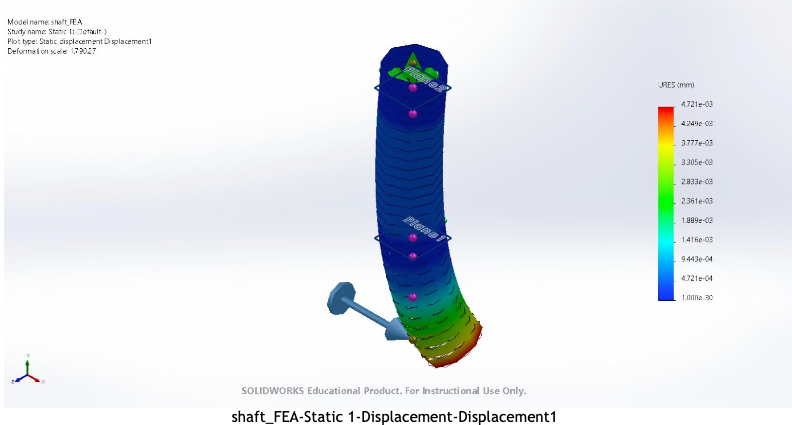
\includegraphics[width=0.75\textwidth]{fig_shaft_fea_displacement}
    \caption{ผล FEA เพลา: ระยะการเบี่ยงเบน (URES Displacement)
             (Max $= 4.721 \times 10^{-3}$\,mm ที่ปลายเพลา)}
    \label{fig:shaft_fea_displacement}
\end{figure}

% -----------------------------------------------------------------------
% รูปที่: Shaft FEA — Factor of Safety
% ชื่อไฟล์แนะนำ: fig_shaft_fea_fos.png
% เนื้อหา: SOLIDWORKS FOS color map
%          Min FOS = 9.313 ที่ Node 5 (บริเวณ Belt Pulley)
%          แสดง scale ด้านขวา พร้อม label Min FOS
% -----------------------------------------------------------------------
\begin{figure}[H]
    \centering
    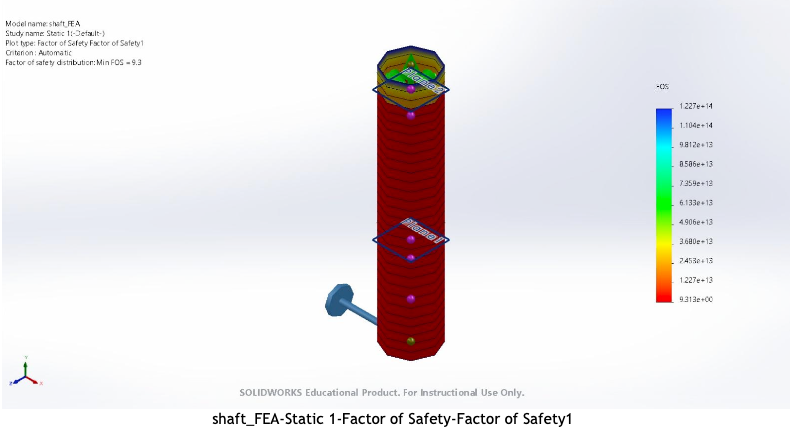
\includegraphics[width=0.75\textwidth]{fig_shaft_fea_fos}
    \caption{ผล FEA เพลา: ค่าความปลอดภัย (Factor of Safety)
             (Min FOS $= 9.313$ บริเวณตำแหน่ง Belt Pulley)}
    \label{fig:shaft_fea_fos}
\end{figure}

% -----------------------------------------------------------------------
% รูปที่: Shaft FEA — Shear Force Diagram
% ชื่อไฟล์แนะนำ: fig_shaft_fea_shear.png
% เนื้อหา: SOLIDWORKS Shear Force in Dir2 diagram
%          แสดง shear diagram ตามความยาวเพลา
%          Max shear = 88.12 N ในช่วง Belt Pulley
% -----------------------------------------------------------------------
\begin{figure}[H]
    \centering
    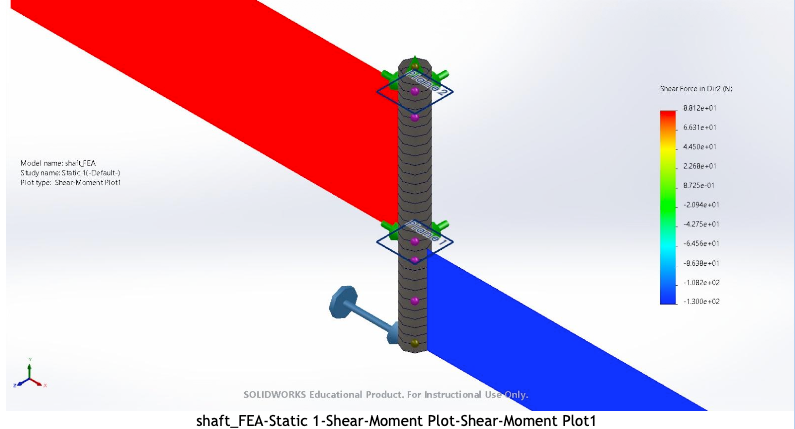
\includegraphics[width=0.75\textwidth]{fig_shaft_fea_shear}
    \caption{ผล FEA เพลา: แผนภาพแรงเฉือน (Shear Force in Dir2)
             แสดงการเปลี่ยนแปลงแรงเฉือนตลอดความยาวเพลา}
    \label{fig:shaft_fea_shear}
\end{figure}

% -----------------------------------------------------------------------
% รูปที่: Shaft FEA — Bending Moment Diagram
% ชื่อไฟล์แนะนำ: fig_shaft_fea_moment.png
% เนื้อหา: SOLIDWORKS Moment about Dir2 diagram
%          Max moment = 1.7 N.m ที่ Fixture ด้านบน
%          แสดง moment diagram ตามความยาวเพลา
% -----------------------------------------------------------------------
\begin{figure}[H]
    \centering
    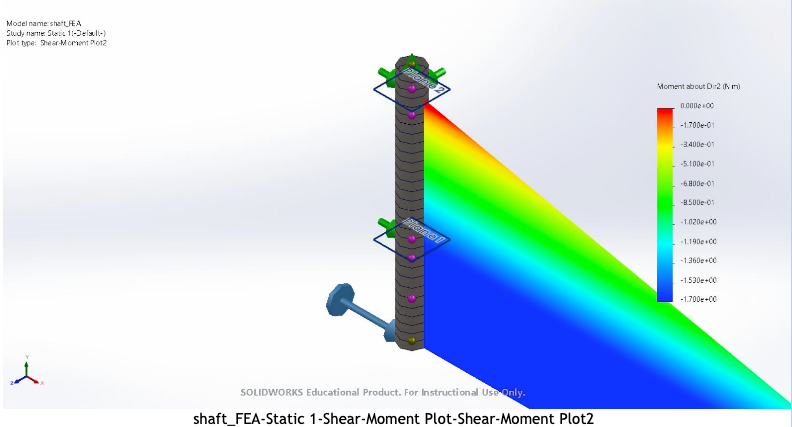
\includegraphics[width=0.75\textwidth]{fig_shaft_fea_moment}
    \caption{ผล FEA เพลา: แผนภาพโมเมนต์ดัด (Bending Moment about Dir2)
             แสดงการกระจาย Bending Moment ตลอดความยาวเพลา}
    \label{fig:shaft_fea_moment}
\end{figure}

\subsubsection{การตรวจสอบความสอดคล้องกับการคำนวณเชิงวิเคราะห์}

\begin{table}[H]
  \centering
  \caption{สรุปผลการวิเคราะห์ FEA เพลาเทียบกับการคำนวณ ASME Code}
  \label{tab:shaft_fea_results}
  \begin{tabular}{lcccc}
    \toprule
    พารามิเตอร์ & ผล FEA & เกณฑ์ & หน่วย & ผล \\
    \midrule
    Max Bending+Axial Stress & $2.221 \times 10^7$ & $< 2.068 \times 10^8$
      & N/m$^2$ & \textbf{ผ่าน} \\
    Max Displacement (URES)  & $4.721 \times 10^{-3}$ & --
      & mm & -- \\
    Min Factor of Safety     & 9.313 & $> 2.0$
      & -- & \textbf{ผ่าน} \\
    \bottomrule
  \end{tabular}
\end{table}

ผล FEA ยืนยันผลการคำนวณ ASME Code ใน\cref{subsec:shaft_calc}
โดย Min FOS = 9.313 สูงกว่าที่คำนวณได้จาก $d_{min} = 10.59$\,mm
เนื่องจากเส้นผ่าศูนย์กลางจริงที่จุดวิกฤต $d_{actual} = 17$\,mm
มี Margin สูงกว่าค่าขั้นต่ำอย่างมาก
Max Displacement เพียง $4.721 \times 10^{-3}$\,mm
บ่งชี้ว่าเพลามีความแข็งเกร็งเพียงพอ
และการโก่งตัวของเพลาจะไม่ส่งผลต่อ Alignment
ของ Encoder ที่ติดตั้งที่ Output Shaft
ซึ่งเป็นปัจจัยสำคัญต่อความแม่นยำของ Closed-loop Control (A1, A2)

% -----------------------------------------------------------------------
% รูปที่: Step Shaft Drawing
% ชื่อไฟล์แนะนำ: fig_shaft_drawing.png
% เนื้อหา: Engineering drawing แสดงขนาดแต่ละช่วง (17/12/8-10 mm)
%          ตำแหน่ง Bearing Seat, Key slot และ Shoulder
% -----------------------------------------------------------------------
\begin{figure}[H]
    \centering
    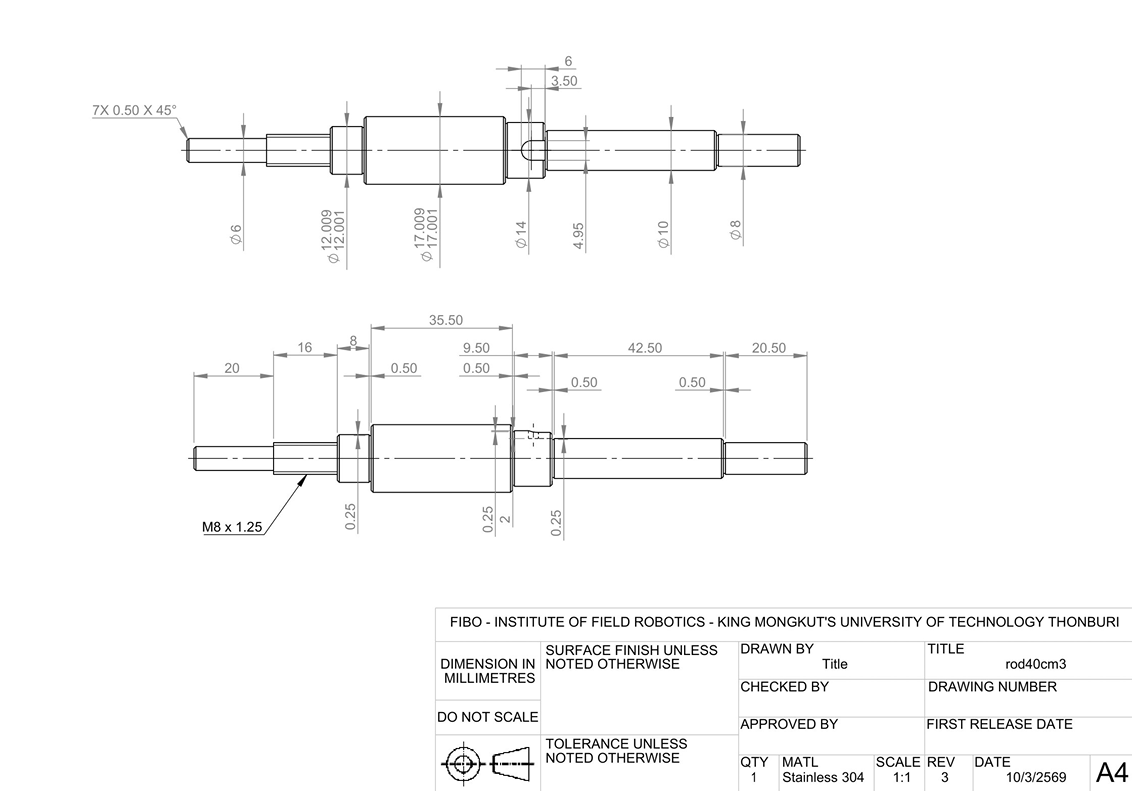
\includegraphics[width=0.85\textwidth]{fig_shaft_drawing}
    \caption{Step Shaft Drawing แสดงขนาดเพลาแต่ละช่วงและตำแหน่งลูกปืน}
    \label{fig:shaft_drawing}
\end{figure}

% -----------------------------------------------------------------------
\subsection{การคำนวณสายพาน}
\label{subsec:belt_calc}
% -----------------------------------------------------------------------

ระบบเลือกใช้สายพาน HTD5M (High Torque Drive, 5\,mm Pitch)
แทน XL หรือ GT2 เนื่องจาก Curvilinear Tooth Profile ของ HTD
ออกแบบมาเฉพาะสำหรับ High Torque Low Speed Application
โดยกระจายแรงกดที่ฟันสายพานได้สม่ำเสมอกว่า Trapezoidal Profile
ของ XL ซึ่งมีความเสี่ยง Tooth Jump เมื่อ Tight Side Tension สูง

\subsubsection{ค่าเริ่มต้นของระบบสายพาน}

\begin{table}[H]
  \centering
  \caption{ค่าเริ่มต้นของระบบสายพาน HTD5M}
  \label{tab:belt_initial}
  \begin{tabular}{llll}
    \toprule
    พารามิเตอร์ & สัญลักษณ์ & ค่า & หน่วย \\
    \midrule
    ประเภทสายพาน    & --        & HTD5M (Steel Cord, Joined Endless) & -- \\
    ความกว้างสายพาน & $b_0$     & 15    & mm \\
    Belt Pitch      & $P_b$     & 5     & mm \\
    Driver Pulley   & $z_1$     & 24    & teeth \\
    Driven Pulley   & $z_2$     & 70    & teeth \\
    ระยะศูนย์กลาง   & $e$       & 181.25 & mm \\
    แรงบิดที่แขนกล  & $T_{arm}$ & 8.3279 & N$\cdot$m \\
    อัตราทด         & $i$       & 2.917 & -- \\
    \bottomrule
  \end{tabular}
\end{table}

\subsubsection{Peripheral Force}

\begin{equation}
  d_1 = \frac{z_1 P_b}{\pi} = \frac{24 \times 5}{\pi} = 38.20\,\text{mm}, \qquad
  d_2 = \frac{z_2 P_b}{\pi} = \frac{70 \times 5}{\pi} = 111.41\,\text{mm}
  \label{eq:belt_diameters}
\end{equation}

\begin{equation}
  F_U = \frac{2\,T_{driver}}{d_1}
      = \frac{2 \times 2.855}{0.03820}
      = 130\,\text{N}
  \label{eq:belt_fu}
\end{equation}

ค่า Admissible Peripheral Force ของ HTD5M ขนาด 15\,mm
จาก Habasit Catalog คือ 400\,N
ดังนั้น $F_U = 130\,\text{N} \ll 400\,\text{N}$ \textbf{(ผ่าน)}
ความกว้าง 15\,mm เกินค่าขั้นต่ำที่คำนวณได้ ($b_{req} = 3.9$\,mm)
อย่างมีนัยสำคัญ เพื่อรองรับ Misalignment ที่อาจเกิดขึ้นใน
การประกอบจริง และลดความเสี่ยง Edge Wear ของสายพาน

\begin{figure}[H]
    \centering
    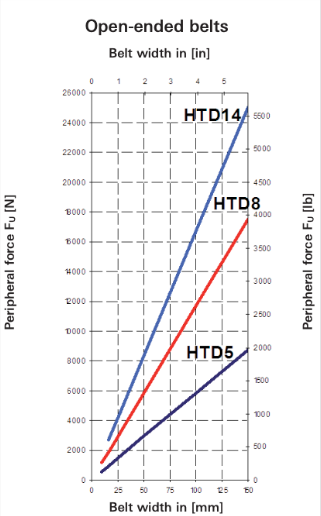
\includegraphics[width=0.5\textwidth]{fig_habasit_catalog}
    \caption{ตารางค่า Admissible Peripheral Force ของสายพาน HTD5M
             จาก Habasit Engineering Guide แสดงพิกัด 400\,N
             สำหรับความกว้าง 15\,mm}
    \label{fig:habasit_catalog}
\end{figure}


\subsubsection{Belt Length และ Teeth in Mesh}

\begin{equation}
  z_b = \frac{2e}{P_b} + \frac{z_1+z_2}{2}
      + \frac{P_b}{4e}\!\left(\frac{z_2-z_1}{\pi}\right)^2
      = 119\,\text{teeth}, \qquad
  l_0 = z_b \times P_b = 595\,\text{mm}
  \label{eq:belt_length}
\end{equation}

\begin{equation}
  z_m = z_1\!\left(0.5 - \frac{d_2-d_1}{2\pi e}\right)
      = 6.74\,\text{teeth} > 5
  \quad\Rightarrow\quad t_m = 1.0\;\textbf{(ผ่าน)}
  \label{eq:belt_zm}
\end{equation}

\subsubsection{Belt Tension และ Width Verification}

\begin{equation}
  F_1 = F_2 + F_U = 26 + 130 = 156\,\text{N (Tight Side)}, \qquad
  F_2 = 26\,\text{N (Slack Side)}
  \label{eq:belt_tension}
\end{equation}

\begin{table}[H]
  \centering
  \caption{สรุปผลการคำนวณสายพาน HTD5M}
  \label{tab:belt_summary}
  \begin{tabular}{lcccc}
    \toprule
    พารามิเตอร์ & ผลคำนวณ & เกณฑ์ & หน่วย & ผล \\
    \midrule
    Peripheral Force $F_U$ & 130  & $\leq 400$ & N     & \textbf{ผ่าน} \\
    Teeth in Mesh $z_m$    & 6.74 & $> 5$      & teeth & \textbf{ผ่าน} \\
    Belt Width $b_0$        & 15   & $\geq 3.9$ & mm    & \textbf{ผ่าน} \\
    Belt Length $l_0$       & 595  & --         & mm    & -- \\
    Tight Side Tension $F_1$ & 156 & --         & N     & -- \\
    Slack Side Tension $F_2$ & 26  & --         & N     & -- \\
    \bottomrule
  \end{tabular}
\end{table}

% -----------------------------------------------------------------------
\subsection{การเลือกตลับลูกปืนและการคำนวณอายุการใช้งาน}
\label{subsec:bearing_calc}
% -----------------------------------------------------------------------

เลือกตลับลูกปืน 2 ตำแหน่งโดยอ้างอิงมาตรฐาน ISO~281
ที่ความเร็วรอบ 85\,RPM

ลูกปืนบน (SKF~30203, Tapered Roller) เลือกเพราะต้องรับทั้ง
Radial Load จากแรงดึงสายพานและ Axial Load จากน้ำหนักแขนกล
พร้อมกัน ซึ่ง Tapered Roller Bearing รับ Combined Load
ได้ดีกว่า Deep Groove Ball Bearing ที่ขนาด Bore เดียวกัน
ลูกปืนล่าง (F6901ZZ, Deep Groove Ball) รับเฉพาะ
Radial Load เป็นหลักจึงเลือก Ball Bearing ที่มีแรงเสียดทานต่ำกว่า

\begin{table}[H]
  \centering
  \caption{ผลการคำนวณอายุการใช้งานของตลับลูกปืน}
  \label{tab:bearing_life}
  \begin{tabular}{lcccc}
    \toprule
    ตำแหน่ง / รุ่น & $C$ (kN) & $P$ (kN) & $L_{10h}$ (ชั่วโมง) & ผล \\
    \midrule
    SKF 30203 (Taper Roller, ลูกปืนบน)     & 23.400 & 0.2600
      & $6.1 \times 10^8$ & \textbf{ผ่าน} \\
    F6901ZZ (Deep Groove Ball, ลูกปืนล่าง) & 2.886  & 0.1388
      & $1.76 \times 10^6$ & \textbf{ผ่าน} \\
    \bottomrule
    \multicolumn{5}{l}{\small เกณฑ์มาตรฐานทั่วไปสำหรับเครื่องจักรกล:
      20,000--100,000 ชั่วโมง}\\
  \end{tabular}
\end{table}

\subsection{การวิเคราะห์การโก่งตัวด้วย FEA}
\label{subsec:fea}

ดำเนินการวิเคราะห์ Finite Element Analysis (Static Study)
ด้วย SOLIDWORKS Simulation ภายใต้โหลด 2\,kg ตามข้อกำหนด M3
วัสดุแขนกลเลือกใช้ Galvanized Steel แทน Stainless Steel AISI~304
เนื่องจากน้ำหนักที่เบากว่าช่วยลดโมเมนต์ความเฉื่อย $J$ ของส่วนที่หมุน
ซึ่งส่งผลโดยตรงต่อ Torque Budget และ Cycle Time (P1)
โดยยอมรับ Trade-off ด้าน Corrosion Resistance ที่ต่ำกว่า
เนื่องจากสภาพแวดล้อมการใช้งานเป็น Indoor Industrial

\subsubsection{สภาวะการจำลอง (FEA Setup)}

กำหนด Boundary Conditions ดังนี้

\begin{itemize}
  \item \textbf{Fixture:} Fixed Geometry ที่ขอบรูน็อตทั้งสองฝั่ง
        และหน้าสัมผัสที่แนบกับตัวฐานหุ่นยนต์
  \item \textbf{Load:} Remote Load 2.76\,kg ที่หน้าสัมผัสปลายแขน
        (ตำแหน่ง $x = -0.9$\,mm, $y = -46.82$\,mm, $z = 55.58$\,mm)
        โดยใช้ Remote Load แทน Point Load
        เพื่อกระจายแรงผ่าน Remote Point
        ตามน้ำหนักจริงของ Gripper และ Connection Rod รวมกัน
  \item \textbf{Mesh:} Solid, Blended Curvature-based,
        High Quality (Jacobian 16 Points),
        11,607 Nodes, 5,722 Elements
\end{itemize}

% -----------------------------------------------------------------------
% รูปที่: FEA Setup — Fixture และ Load Direction
% ชื่อไฟล์แนะนำ: fig_fea_setup_fixture.png
% เนื้อหา: SOLIDWORKS screenshot แสดงจุดจับยึด (สีฟ้า)
%          และทิศทางของภาระแรง (ลูกศรสีชมพู)
% -----------------------------------------------------------------------
\begin{figure}[H]
    \centering
    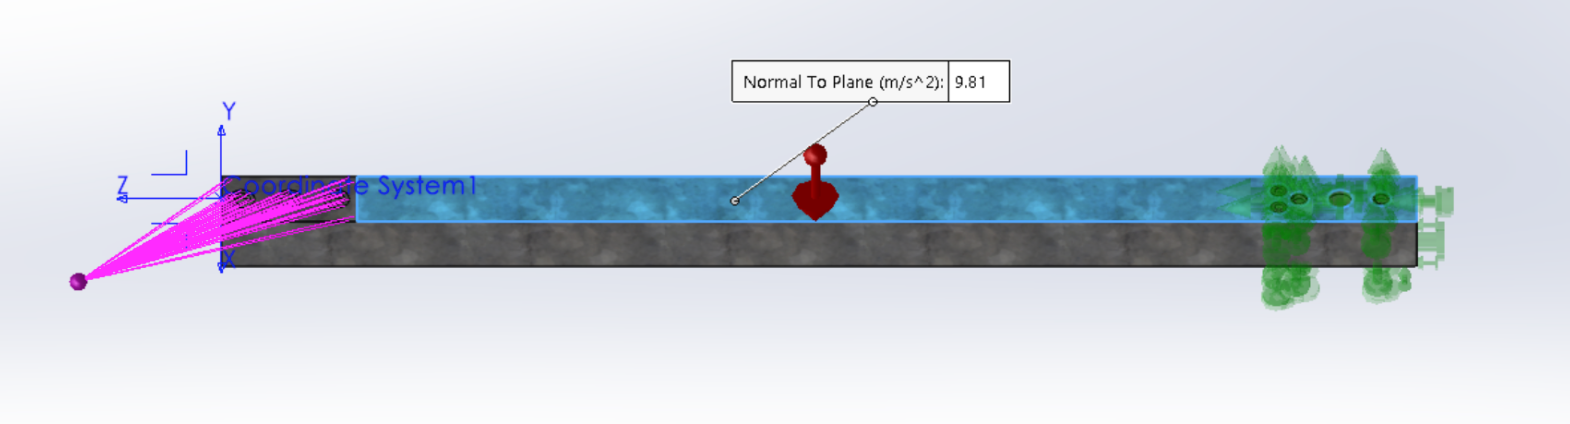
\includegraphics[width=0.82\textwidth]{fig_fea_setup_fixture}
    \caption{โมเดลจำลอง FEA แสดงจุดจับยึด Fixture (สีฟ้า)
             และทิศทางของภาระแรง Remote Load (ลูกศรสีชมพู)}
    \label{fig:fea_setup_fixture}
\end{figure}

% -----------------------------------------------------------------------
% รูปที่: FEA Setup — Remote Load Parameters
% ชื่อไฟล์แนะนำ: fig_fea_setup_remoteload.png
% เนื้อหา: SOLIDWORKS screenshot แสดง Remote Mass = 2.76 kg
%          พร้อม coordinate ของ Remote Point
% -----------------------------------------------------------------------
\begin{figure}[H]
    \centering
    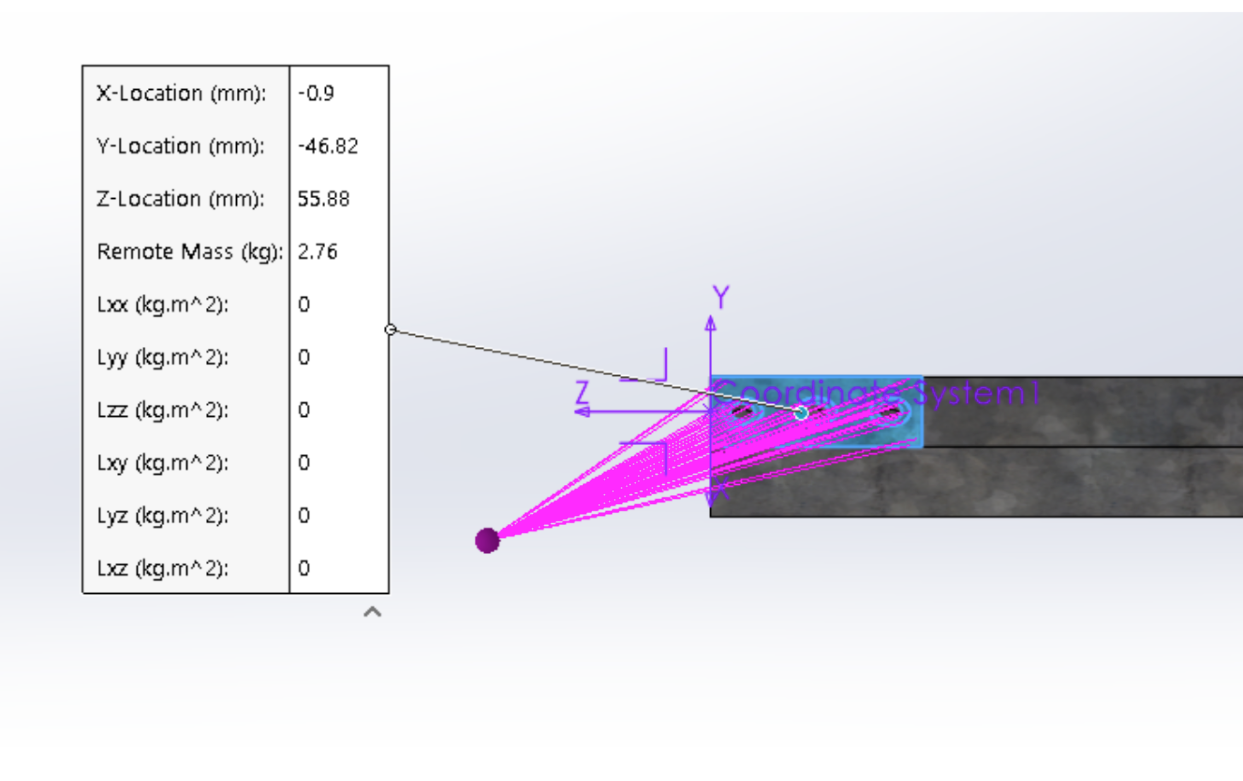
\includegraphics[width=0.82\textwidth]{fig_fea_setup_remoteload}
    \caption{การตั้งค่า Remote Load 2.76\,kg แสดง Remote Point
             และ Moment of Inertia ที่กำหนด}
    \label{fig:fea_setup_remoteload}
\end{figure}

\subsubsection{การตรวจสอบเชิงวิเคราะห์ก่อน FEA (Analytical Verification)}

ก่อนดำเนินการ FEA ทำการตรวจสอบเบื้องต้นด้วยการคำนวณเชิงวิเคราะห์
โดยจำลองแขนกลเป็น Cantilever Beam หน้าตัด Galvanized Square Tube
$25 \times 25$\,mm หนา 1.4\,mm ความยาว $L = 0.5$\,m

Second Moment of Inertia ของหน้าตัดท่อสี่เหลี่ยม

\begin{equation}
  I = \frac{bh^3 - b_i h_i^3}{12}
    = \frac{25 \times 25^3 - 20.4 \times 20.4^3}{12}
    = 18{,}119.65\,\text{mm}^4
  \label{eq:arm_inertia}
\end{equation}

การโก่งตัวแบ่งออกเป็น 2 ส่วน ได้แก่
การโก่งจากน้ำหนักแขนกลเอง (Distributed Load $w$)
และการโก่งจากโหลดที่ปลายแขน (Point Load $P$)

\begin{align}
  \delta_1 &= \frac{wL^4}{8EI}
            = \frac{5.123 \times 0.5^4}
                   {8 \times 200{,}000 \times 18{,}119.65 \times 10^{-12}}
            = 0.0110\,\text{mm}
  \label{eq:deflection_dist} \\[6pt]
  \delta_2 &= \frac{PL^3}{3EI}
            = \frac{19.62 \times 0.5^3}
                   {3 \times 200{,}000 \times 18{,}119.65 \times 10^{-12}}
            = 0.2256\,\text{mm}
  \label{eq:deflection_point}
\end{align}

การโก่งตัวรวม

\begin{equation}
  \delta_{total} = \delta_1 + \delta_2
                = 0.0110 + 0.2256
                = 0.2366\,\text{mm} < 1.0\,\text{mm}
                \quad\textbf{(ผ่าน)}
  \label{eq:deflection_total}
\end{equation}

\subsubsection{ผลการวิเคราะห์ FEA}

\begin{table}[H]
  \centering
  \caption{คุณสมบัติวัสดุที่ใช้ใน FEA (Galvanized Steel)}
  \label{tab:fea_material}
  \begin{tabular}{lll}
    \toprule
    คุณสมบัติ & ค่า & หน่วย \\
    \midrule
    Yield Strength  & $2.35 \times 10^8$ & N/m$^2$ \\
    Elastic Modulus & $2.00 \times 10^{11}$ & N/m$^2$ \\
    Poisson's Ratio & 0.26 & -- \\
    Mass Density    & 7,850 & kg/m$^3$ \\
    \bottomrule
  \end{tabular}
\end{table}

% -----------------------------------------------------------------------
% รูปที่: Von Mises Stress Distribution
% ชื่อไฟล์แนะนำ: fig_fea_stress.png
% เนื้อหา: SOLIDWORKS color map ของ Von Mises Stress
%          Max = 2.721e+07 N/m² บริเวณขอบหน้าสัมผัสฐาน
%          ระบุจุด Max ด้วย callout
% -----------------------------------------------------------------------
\begin{figure}[H]
    \centering
    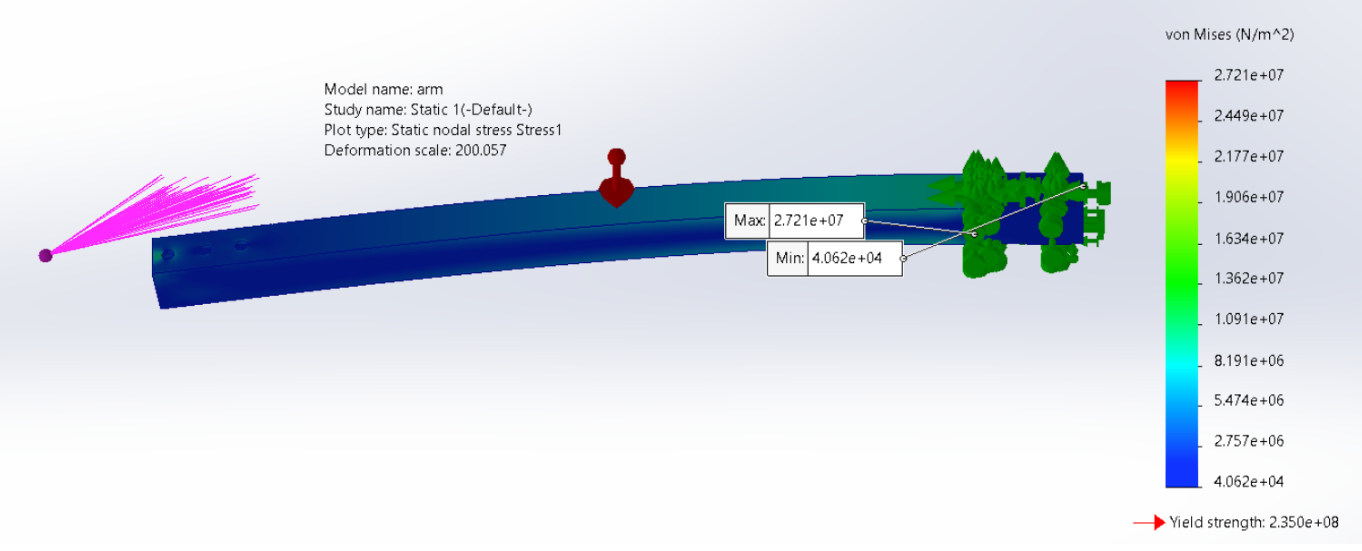
\includegraphics[width=0.82\textwidth]{fig_fea_stress}
    \caption{ผล FEA: การกระจายตัวของ Von Mises Stress บนแขนกล
             (Max $= 2.721 \times 10^7$\,N/m$^2$ บริเวณขอบหน้าสัมผัสกับฐาน)}
    \label{fig:fea_stress}
\end{figure}

% -----------------------------------------------------------------------
% รูปที่: Displacement Distribution
% ชื่อไฟล์แนะนำ: fig_fea_displacement.png
% เนื้อหา: SOLIDWORKS color map ของ URES Displacement
%          Max = 2.337e-01 mm ที่ปลายแขนกล
% -----------------------------------------------------------------------
\begin{figure}[H]
    \centering
    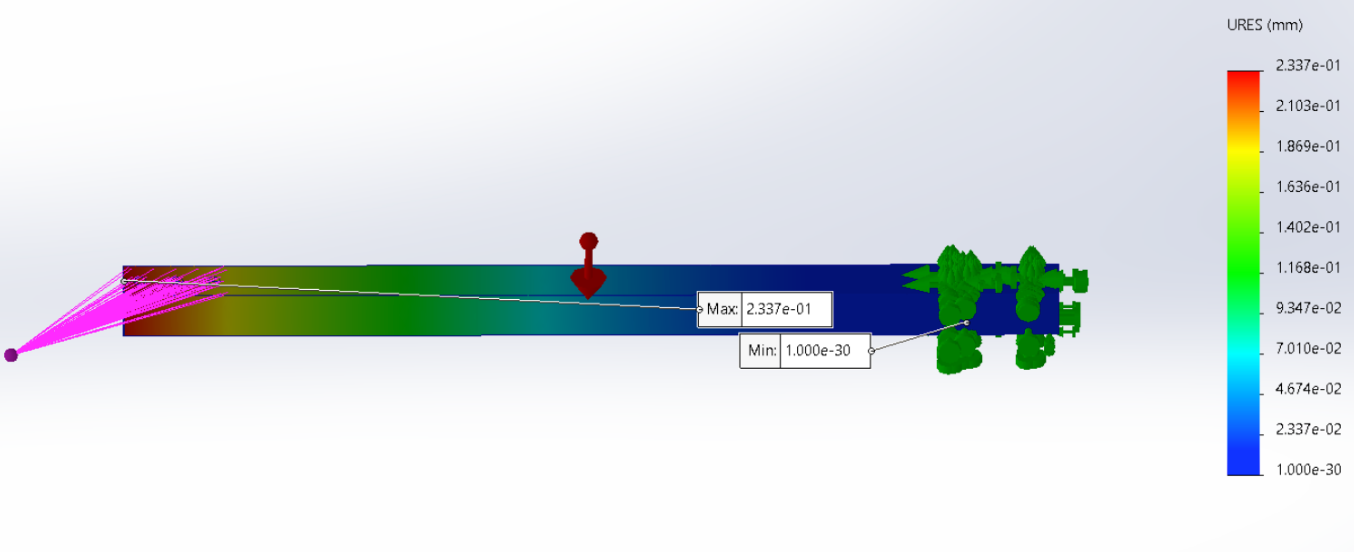
\includegraphics[width=0.82\textwidth]{fig_fea_displacement}
    \caption{ผล FEA: ระยะการแอ่นตัว (Displacement) บนแขนกล
             (Max $= 0.2337$\,mm ที่ปลายสุดของแขนกล)}
    \label{fig:fea_displacement}
\end{figure}

% -----------------------------------------------------------------------
% รูปที่: Factor of Safety Distribution
% ชื่อไฟล์แนะนำ: fig_fea_fos.png
% เนื้อหา: SOLIDWORKS color map ของ FOS
%          Min FOS = 8.6 ที่บริเวณขอบหน้าสัมผัสฐาน
% -----------------------------------------------------------------------
\begin{figure}[H]
    \centering
    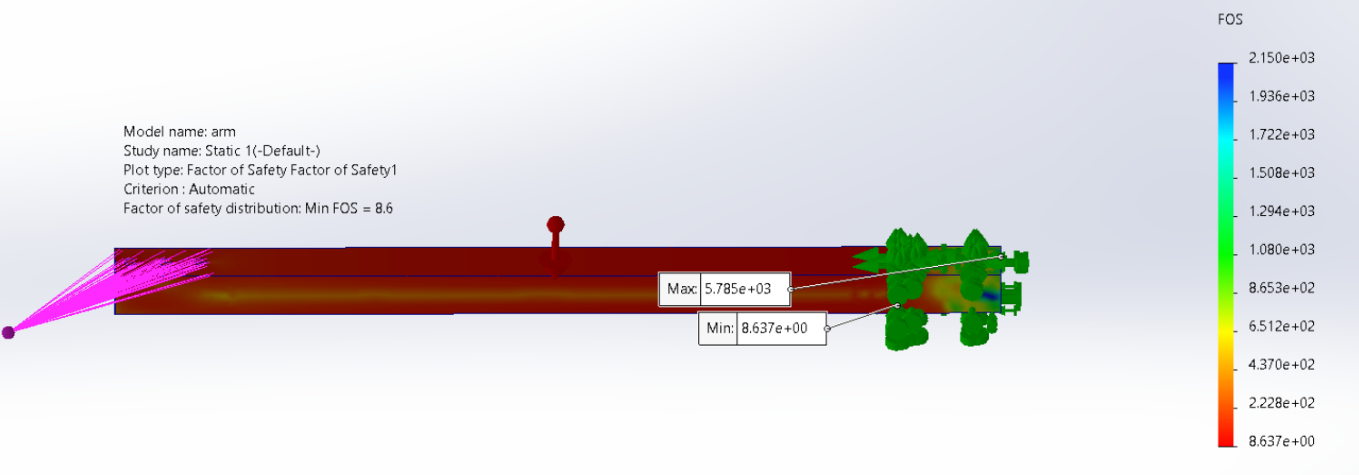
\includegraphics[width=0.82\textwidth]{fig_fea_fos}
    \caption{ผล FEA: ค่าความปลอดภัย (Factor of Safety)
             บนแขนกล (Min FOS $= 8.6$)}
    \label{fig:fea_fos}
\end{figure}

\begin{table}[H]
  \centering
  \caption{สรุปผลการวิเคราะห์ FEA เทียบกับข้อกำหนด M3}
  \label{tab:fea_results}
  \begin{tabular}{lcccc}
    \toprule
    พารามิเตอร์ & ผล FEA & เกณฑ์ & หน่วย & ผล \\
    \midrule
    Max Von Mises Stress & $2.721 \times 10^7$ & $< 2.35 \times 10^8$
      & N/m$^2$ & \textbf{ผ่าน} \\
    Max Displacement (URES) & 0.2337 & $\leq 1.0$
      & mm & \textbf{ผ่าน} \\
    Min Factor of Safety & 8.6 & $> 1.0$
      & -- & \textbf{ผ่าน} \\
    \bottomrule
  \end{tabular}
\end{table}

ผลการคำนวณเชิงวิเคราะห์ ($\delta_{total} = 0.2366$\,mm)
สอดคล้องกับผล FEA ($\delta_{max} = 0.2337$\,mm)
โดยมีความคลาดเคลื่อน $< 2\%$
ซึ่งยืนยันความถูกต้องของแบบจำลอง FEA
ทั้งสองวิธีให้ผลต่ำกว่าเกณฑ์ 1.0\,mm อย่างมีนัยสำคัญ
และ Min FOS $= 8.6 \gg 1.0$ แสดงว่าโครงสร้างมีความแข็งแรง
เพียงพอสำหรับการใช้งานจริงตามข้อกำหนด M3
% ============================================================================
\section{การออกแบบระบบไฟฟ้า}
\label{sec:elec_design}
% ============================================================================

\subsection{สถาปัตยกรรมไฟฟ้าโดยรวม}
\label{subsec:elec_arch}

ระบบไฟฟ้าออกแบบโดยแบ่ง Power Bus ออกเป็น 2 วงจรที่แยกจากกันอย่างชัดเจน
เพื่อให้ E-Stop ตัดเฉพาะกำลังไฟของมอเตอร์ตามข้อกำหนด E6
โดยไม่กระทบต่อการทำงานของ Controller และ Sensor

\textbf{High Power Bus (24\,V/10\,A):}
ไฟ AC 220\,V เข้าผ่าน Circuit Breaker CB1 แล้วจ่ายให้ PSU 24\,V/10\,A
Output ของ PSU ต่อผ่าน NC Contact ของ E-Stop เข้า Magnetic Contactor
เมื่อกด E-Stop สัญญาณ NC Contact เปิดวงจร ทำให้ Contactor
ตัดไฟมอเตอร์ทันทีโดยไม่ผ่าน Firmware (Hardware Fail-Safe)
การเลือกใช้ NC Contact แทน NO Contact
เพื่อให้ระบบ Fail-Safe โดยธรรมชาติ
กล่าวคือหากสายขาดหรือ Coil เสียหาย
Contactor จะตัดไฟโดยอัตโนมัติ

\textbf{Logic Bus (5\,V):}
PSU 5\,V ต่อตรงจาก AC 220\,V \emph{ก่อน} E-Stop Contactor
ทำให้ STM32, ESP32, Encoder, Sensor และ Relay Control Side
มีไฟเลี้ยงตลอดเวลาแม้กด E-Stop
ซึ่งเป็นไปตามข้อกำหนด E6 ที่กำหนดให้ Controller ยังทำงานได้
หลัง E-Stop เพื่อรับ Reset Command และรายงาน Fault Code ผ่าน Modbus

สัญญาณดิจิทัลทุกเส้นระหว่าง High Voltage Side (24\,V)
และ Logic Side (5\,V/3.3\,V) ผ่าน Optocoupler Module 8 ช่อง
เพื่อแยก Ground Loop และป้องกัน Noise จากการสวิตช์ PWM
ของ Motor Driver ไม่ให้ Couple เข้าสู่วงจรลอจิกของ STM32

% -----------------------------------------------------------------------
% รูปที่: Electrical Block Diagram
% ชื่อไฟล์แนะนำ: fig_electric_block.png
% เนื้อหา: Block diagram แสดง 2 Bus แยกกัน (24V และ 5V)
%          E-Stop Contactor คั่นกลาง High Power Bus
%          Optocoupler แยก Signal ระหว่าง 2 domain
%          STM32 และ Sensor อยู่ฝั่ง Logic Bus เสมอ
% -----------------------------------------------------------------------
\begin{figure}[H]
    \centering
    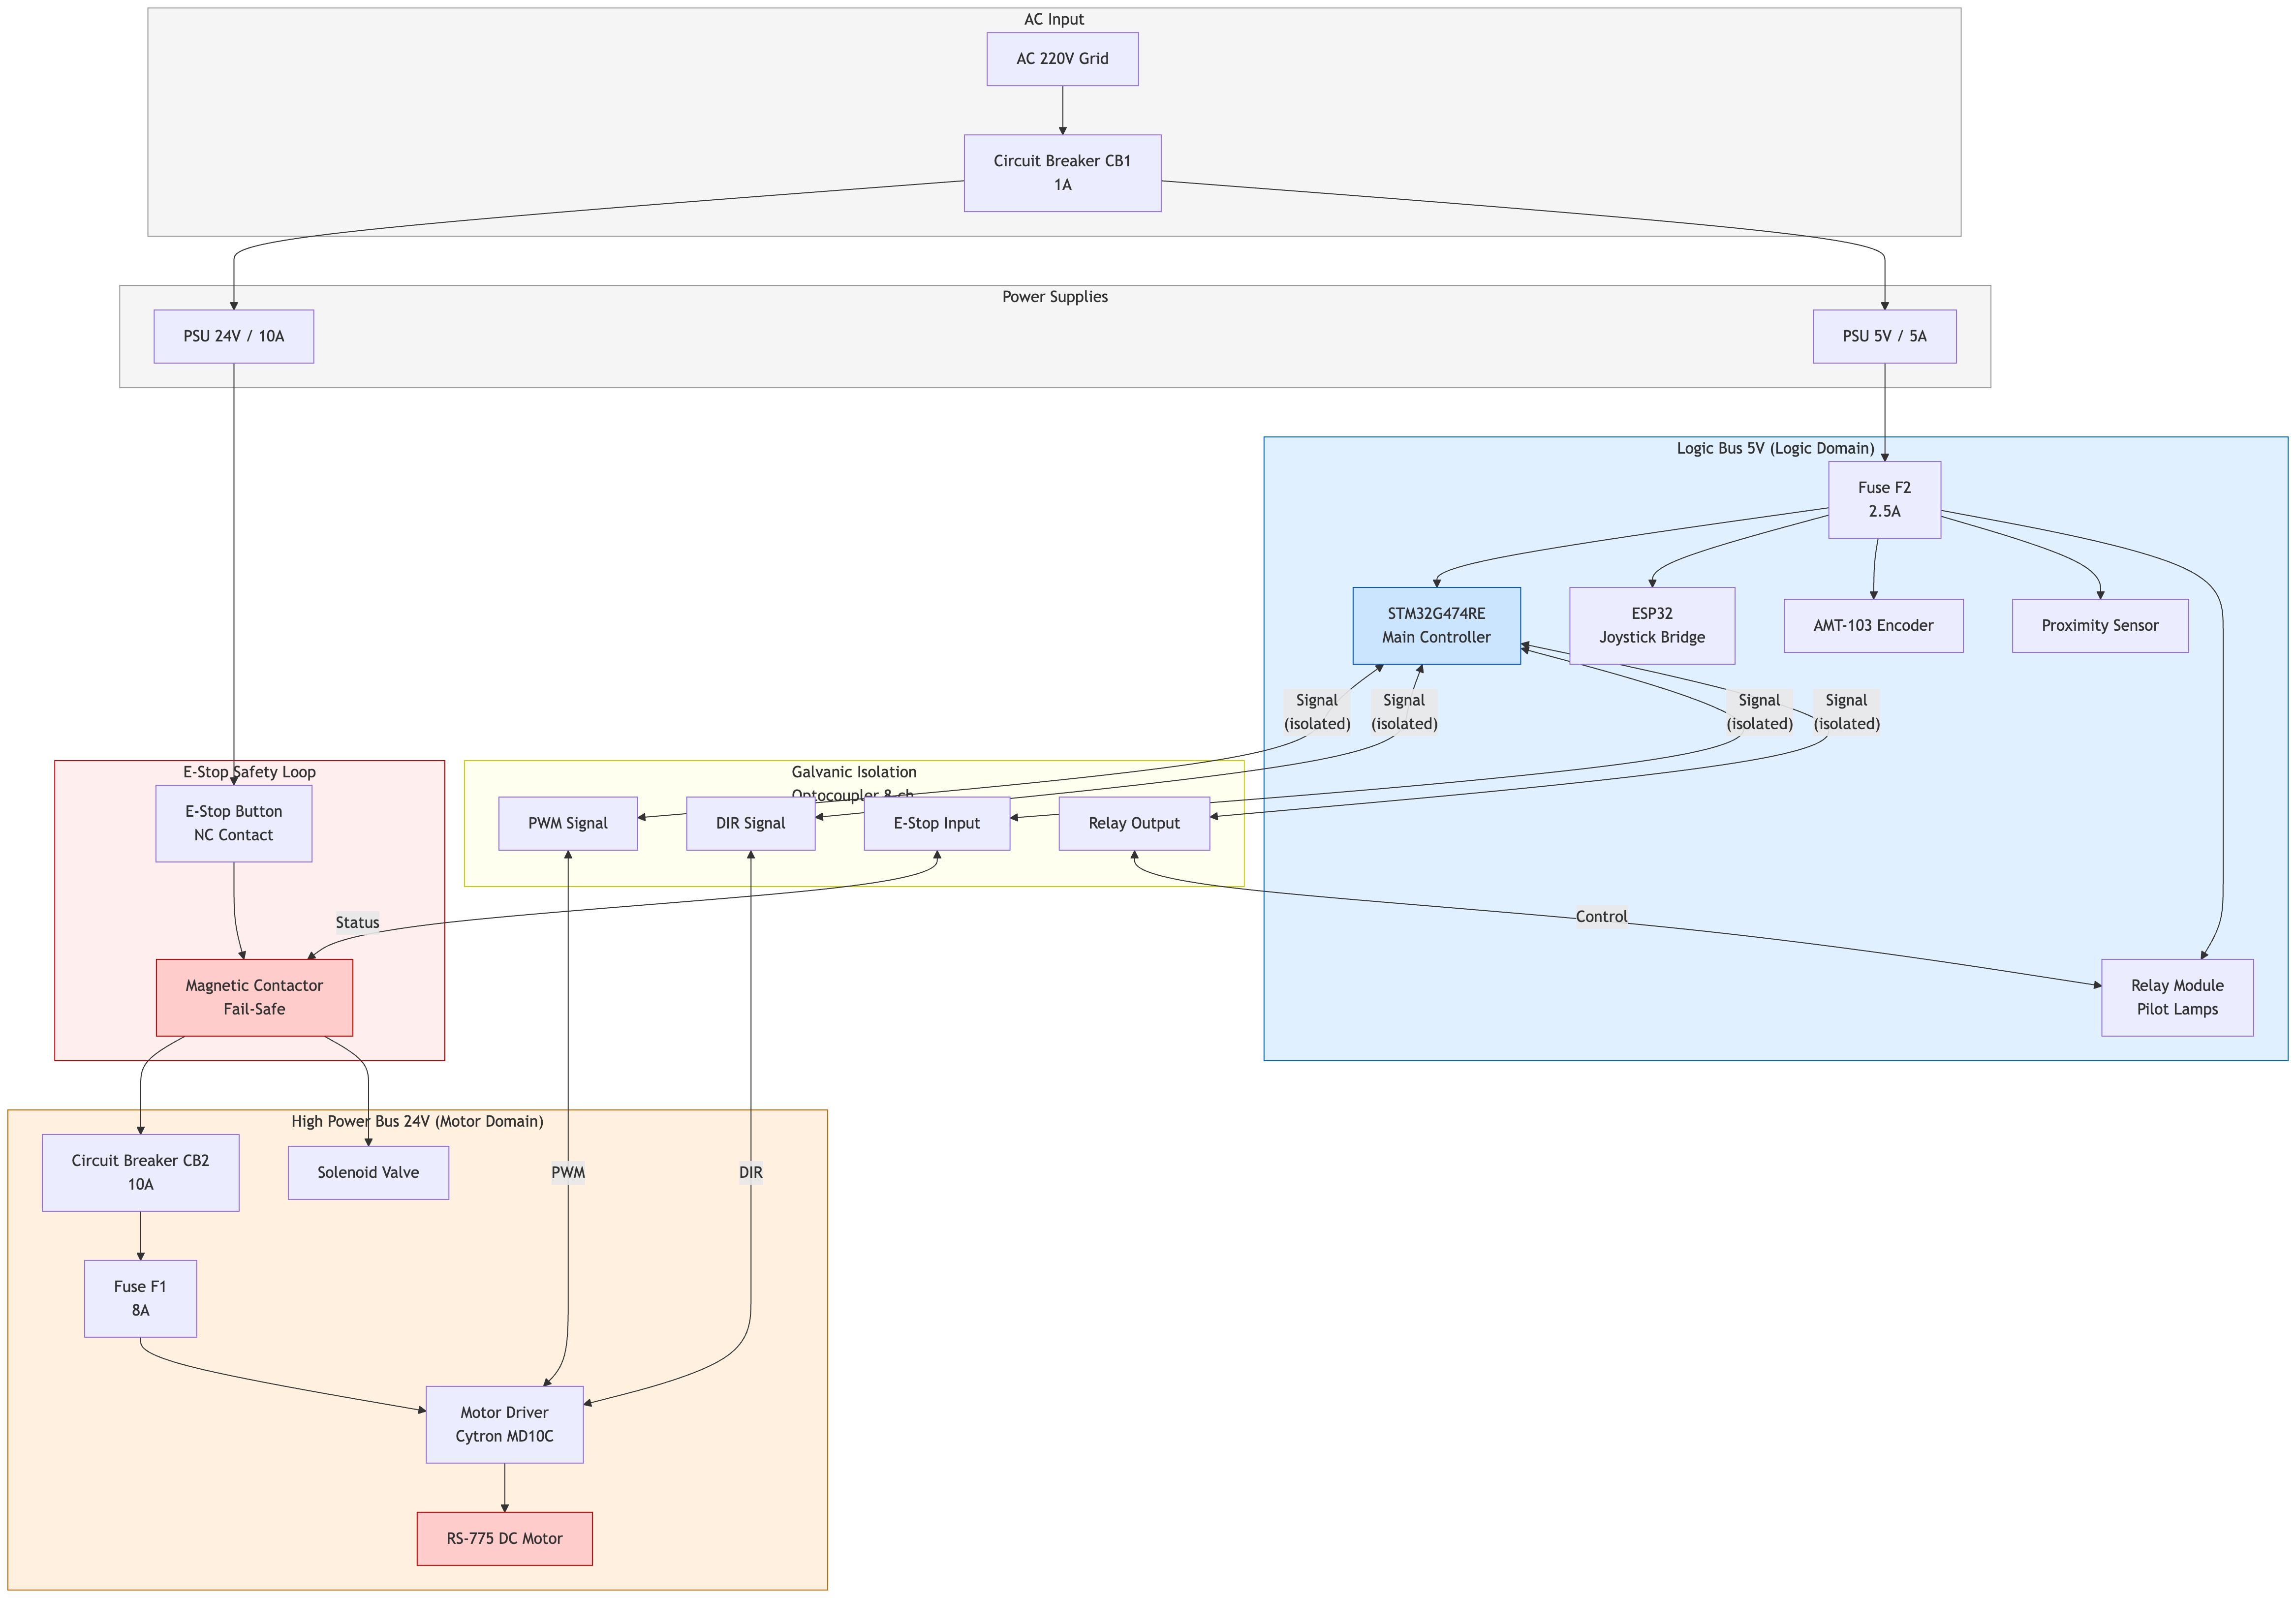
\includegraphics[width=0.95\textwidth]{fig_electric_block}
    \caption{Electrical Block Diagram แสดงการแบ่ง Power Bus
             และการแยก Signal ระหว่าง High Power และ Logic Domain}
    \label{fig:elec_block}
\end{figure}

% -----------------------------------------------------------------------
\subsection{การคำนวณกำลังไฟฟ้าและการเลือก Circuit Breaker}
\label{subsec:power_calc}
% -----------------------------------------------------------------------

\begin{table}[H]
  \centering
  \caption{การคำนวณกำลังไฟฟ้าของ 24\,V Motor Bus}
  \label{tab:power_24v}
  \begin{tabular}{lccr}
    \toprule
    อุปกรณ์ & แรงดัน (V) & กระแสสูงสุด (A) & กำลังไฟฟ้า (W) \\
    \midrule
    DC Motor RS-775    & 24 & 10.00 & 240.00 \\
    Motor Driver MD10C & 24 &  0.10 &   2.40 \\
    Contactor Coil     & 24 &  0.10 &   2.40 \\
    Relay Module       & 24 &  0.20 &   4.80 \\
    Solenoid Valve     & 24 &  0.50 &  12.00 \\
    \midrule
    Safety Margin 20\% & -- &  2.18 &  52.32 \\
    \midrule
    \textbf{รวม 24V Bus} & \textbf{24} & \textbf{13.08} & \textbf{313.92} \\
    \bottomrule
  \end{tabular}
\end{table}

กระแสรวม 13.08\,A เกิน Rating ของ PSU 24\,V/10\,A
อย่างไรก็ตาม Peak Current ของมอเตอร์เกิดขึ้นเพียงช่วงสั้น
ในระหว่าง Acceleration (Current Clamp Zone = 0.71\% ของเวลา)
ระบบจึง Implement Software Current Clamp ใน Firmware
โดยจำกัด Duty Cycle สูงสุดตาม Voltage Budget

\begin{equation}
  D_{max} = \frac{I_{limit} \cdot R_a}{V_{supply}}
           = \frac{8.0 \times 1.4534}{24}
           = 48.4\%
  \label{eq:duty_clamp}
\end{equation}

นอกจากนี้ Safety Stack ใน Firmware ยังตรวจสอบกระแสจริง
จาก WCS1800 Current Sensor แบบ Real-time
โดยหากกระแสเกิน $I_{limit} = 2.0$\,A ต่อเนื่องนานกว่า 100\,ms
ระบบจะ Trigger Fault Code \texttt{0x42} ทันที
เป็น Software Fuse ชั้นที่สองนอกเหนือจาก Hardware Fuse

Safety Margin 20\% เพิ่มเข้าไปเพื่อรองรับ Component Aging
และ Inrush Current ที่อาจสูงกว่าค่า Steady-State
ในช่วง Power-on ของ Solenoid Valve และ Relay Coil

\begin{table}[H]
  \centering
  \caption{การคำนวณกำลังไฟฟ้าของ 5\,V Logic Bus}
  \label{tab:power_5v}
  \begin{tabular}{lccr}
    \toprule
    อุปกรณ์ & แรงดัน (V) & กระแสสูงสุด (A) & กำลังไฟฟ้า (W) \\
    \midrule
    STM32G474RE Nucleo & 5 & 0.50 & 2.50 \\
    ESP32 DevKit V1    & 5 & 0.50 & 2.50 \\
    AMT-103 Encoder    & 5 & 0.10 & 0.50 \\
    Proximity Sensor   & 5 & 0.05 & 0.25 \\
    Optocoupler Module & 5 & 0.04 & 0.20 \\
    Relay Module       & 5 & 0.10 & 0.50 \\
    LED Indicator (×3) & 5 & 0.06 & 0.30 \\
    Selector Switch    & 5 & 0.01 & 0.05 \\
    \midrule
    Safety Margin 20\% & -- & 0.27 & 1.36 \\
    \midrule
    \textbf{รวม 5V Bus} & \textbf{5} & \textbf{1.63} & \textbf{8.16} \\
    \bottomrule
  \end{tabular}
\end{table}

กระแสรวม 1.63\,A $<$ 5\,A ของ PSU 5\,V/5\,A \textbf{(ผ่าน)}

\begin{table}[H]
  \centering
  \caption{การเลือกขนาด Circuit Breaker และ Fuse}
  \label{tab:protection_select}
  \begin{tabular}{llcl}
    \toprule
    อุปกรณ์ & วงจร & กระแสโหลด (A) & ขนาดที่เลือก \\
    \midrule
    Circuit Breaker CB1 & AC Input -- 24V Branch & 0.67  & 1\,A \\
    Circuit Breaker CB2 & DC 24V -- Motor Branch  & 5.28  & 10\,A \\
    Fuse F1             & DC 24V -- Motor         & 5.28  & 8\,A \\
    Fuse F2             & DC 5V -- Logic          & 1.63  & 2.5\,A \\
    \bottomrule
  \end{tabular}
\end{table}

Fuse F1 เลือกขนาด 8\,A ซึ่งต่ำกว่า Rating มอเตอร์ 10\,A
เพื่อให้ Fuse ขาดก่อนที่กระแสจะสูงเกินขีดจำกัดของ
Motor Driver MD10C และ Wiring ภายในตู้ควบคุม
โดยยังมี Software Current Clamp เป็น Protection ชั้นแรก

% -----------------------------------------------------------------------
\subsection{การออกแบบ PCB และวงจรป้องกัน}
\label{subsec:pcb_design}
% -----------------------------------------------------------------------

PCB ออกแบบด้วย KiCad 9.0.0 โดยรวม STM32G474RE Nucleo Board,
ESP32-DEVKITC-32UE, Optocoupler Module 8 ช่อง, Relay Module
และ Connector ทั้งหมดไว้บน Board เดียว
แทนการต่อสายระหว่าง Module แยกกัน
เพื่อลดจำนวน Connector Joint ภายในตู้ควบคุม
ซึ่งเป็นแหล่งหลักของ Intermittent Fault
ในสภาพแวดล้อมที่มีการสั่นสะเทือน

วงจรป้องกันตามข้อกำหนด E7 ออกแบบเป็น 3 ชั้น ดังนี้

\begin{itemize}
  \item \textbf{Hardware Overcurrent Protection:}
        Circuit Breaker CB2 และ Fuse F1 ต่ออนุกรมใน
        24\,V Motor Bus ตัดวงจรเมื่อกระแสเกินพิกัด
        โดยไม่ต้องพึ่ง Firmware
  \item \textbf{Galvanic Isolation:}
        Optocoupler Module แยก Ground ระหว่าง
        High Power Domain (24\,V) และ Logic Domain (5\,V/3.3\,V)
        ทุกเส้นสัญญาณ ป้องกัน Voltage Spike จากการสวิตช์
        PWM ของ Motor Driver ไม่ให้เข้าถึง STM32
  \item \textbf{E-Stop Hardware Interlock:}
        NC Contact ของ E-Stop ต่อ Hard-wired
        ไปยัง Magnetic Contactor โดยตรง
        ไม่ผ่าน Firmware ทำให้ระบบหยุดได้แม้
        STM32 เกิด System Hang
\end{itemize}

% -----------------------------------------------------------------------
% รูปที่: PCB Layout และ 3D Render
% ชื่อไฟล์แนะนำ: fig_pcb_layout.png, fig_pcb_3d.png
% -----------------------------------------------------------------------
\begin{figure}[H]
    \centering
    \begin{subfigure}[b]{0.48\textwidth}
        \centering
        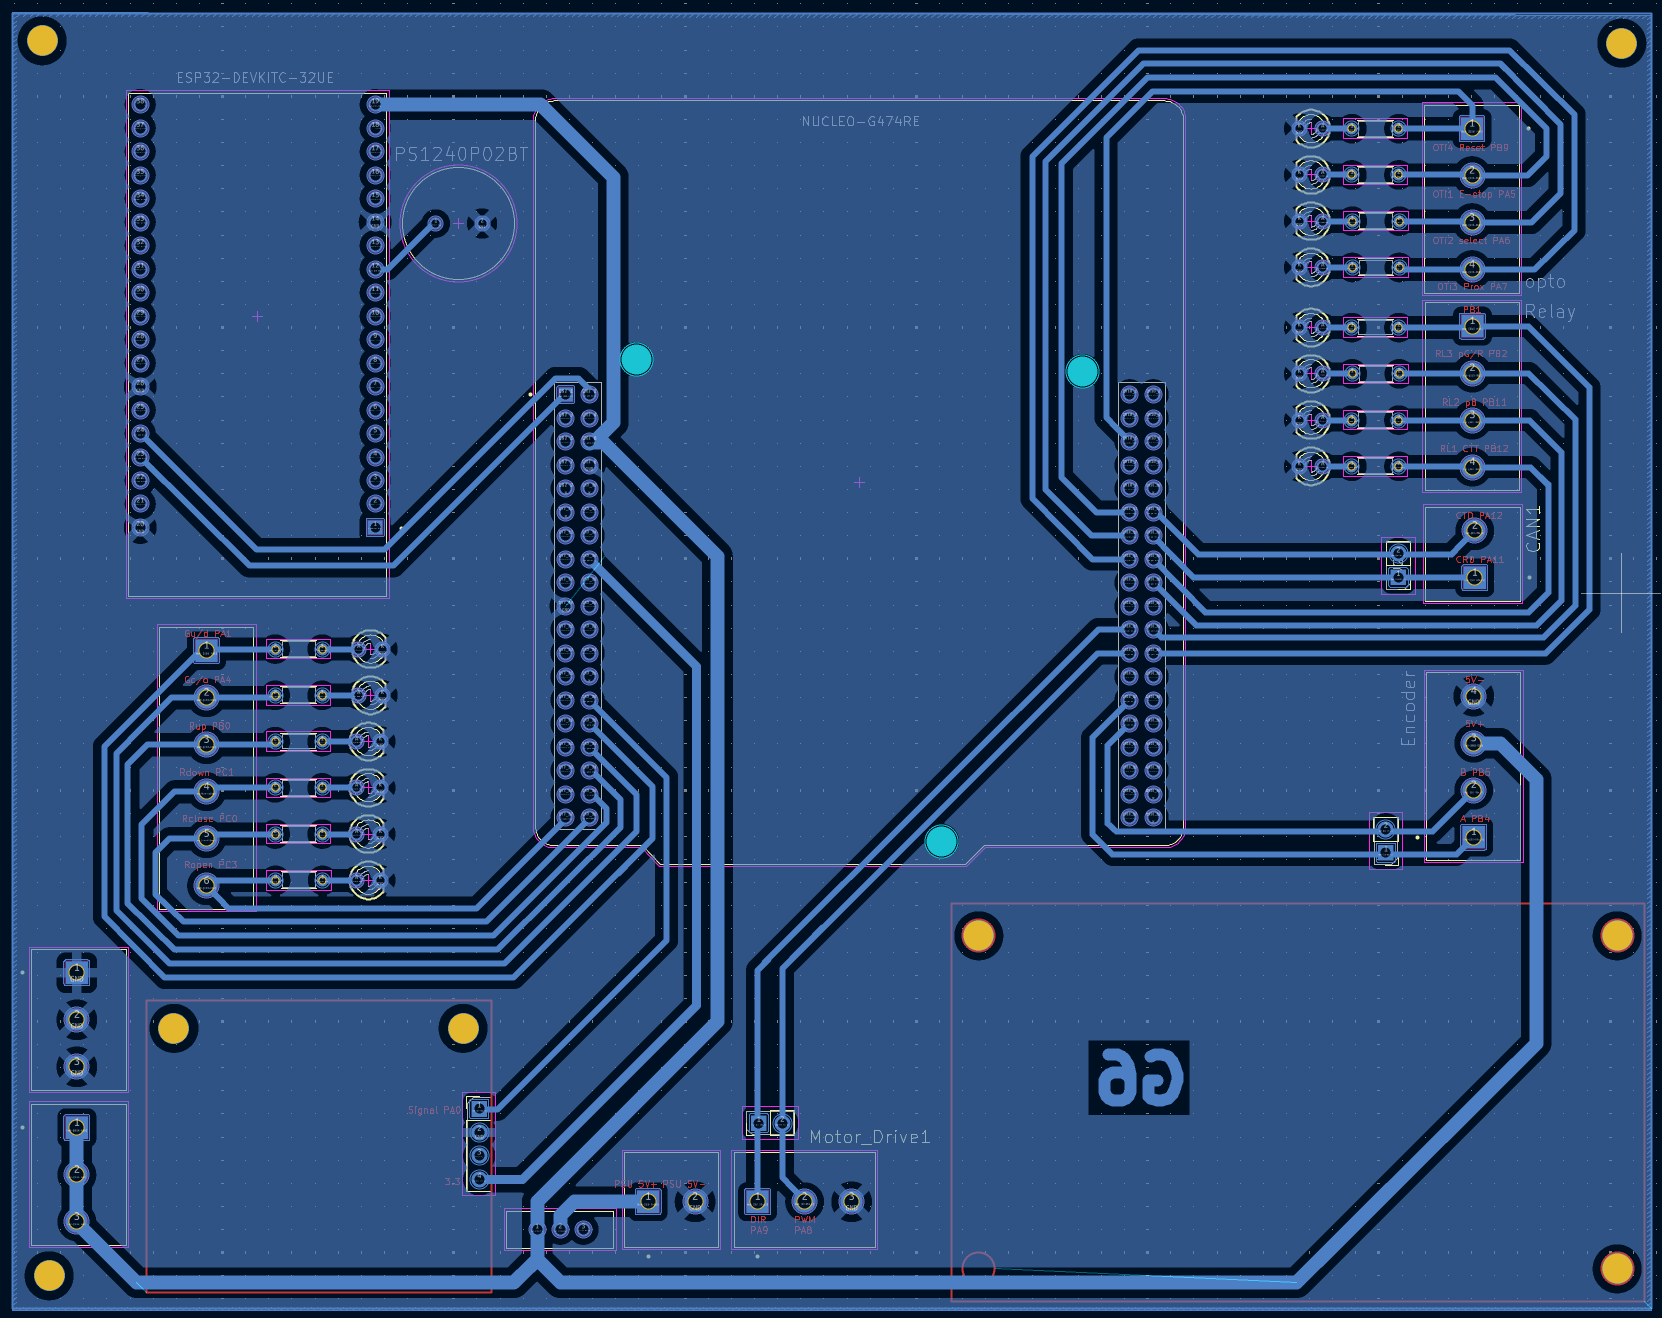
\includegraphics[width=\textwidth]{fig_pcb_layout}
        \caption{PCB Layout (KiCad 9.0.0)}
        \label{fig:pcb_layout}
    \end{subfigure}
    \hfill
    \begin{subfigure}[b]{0.48\textwidth}
        \centering
        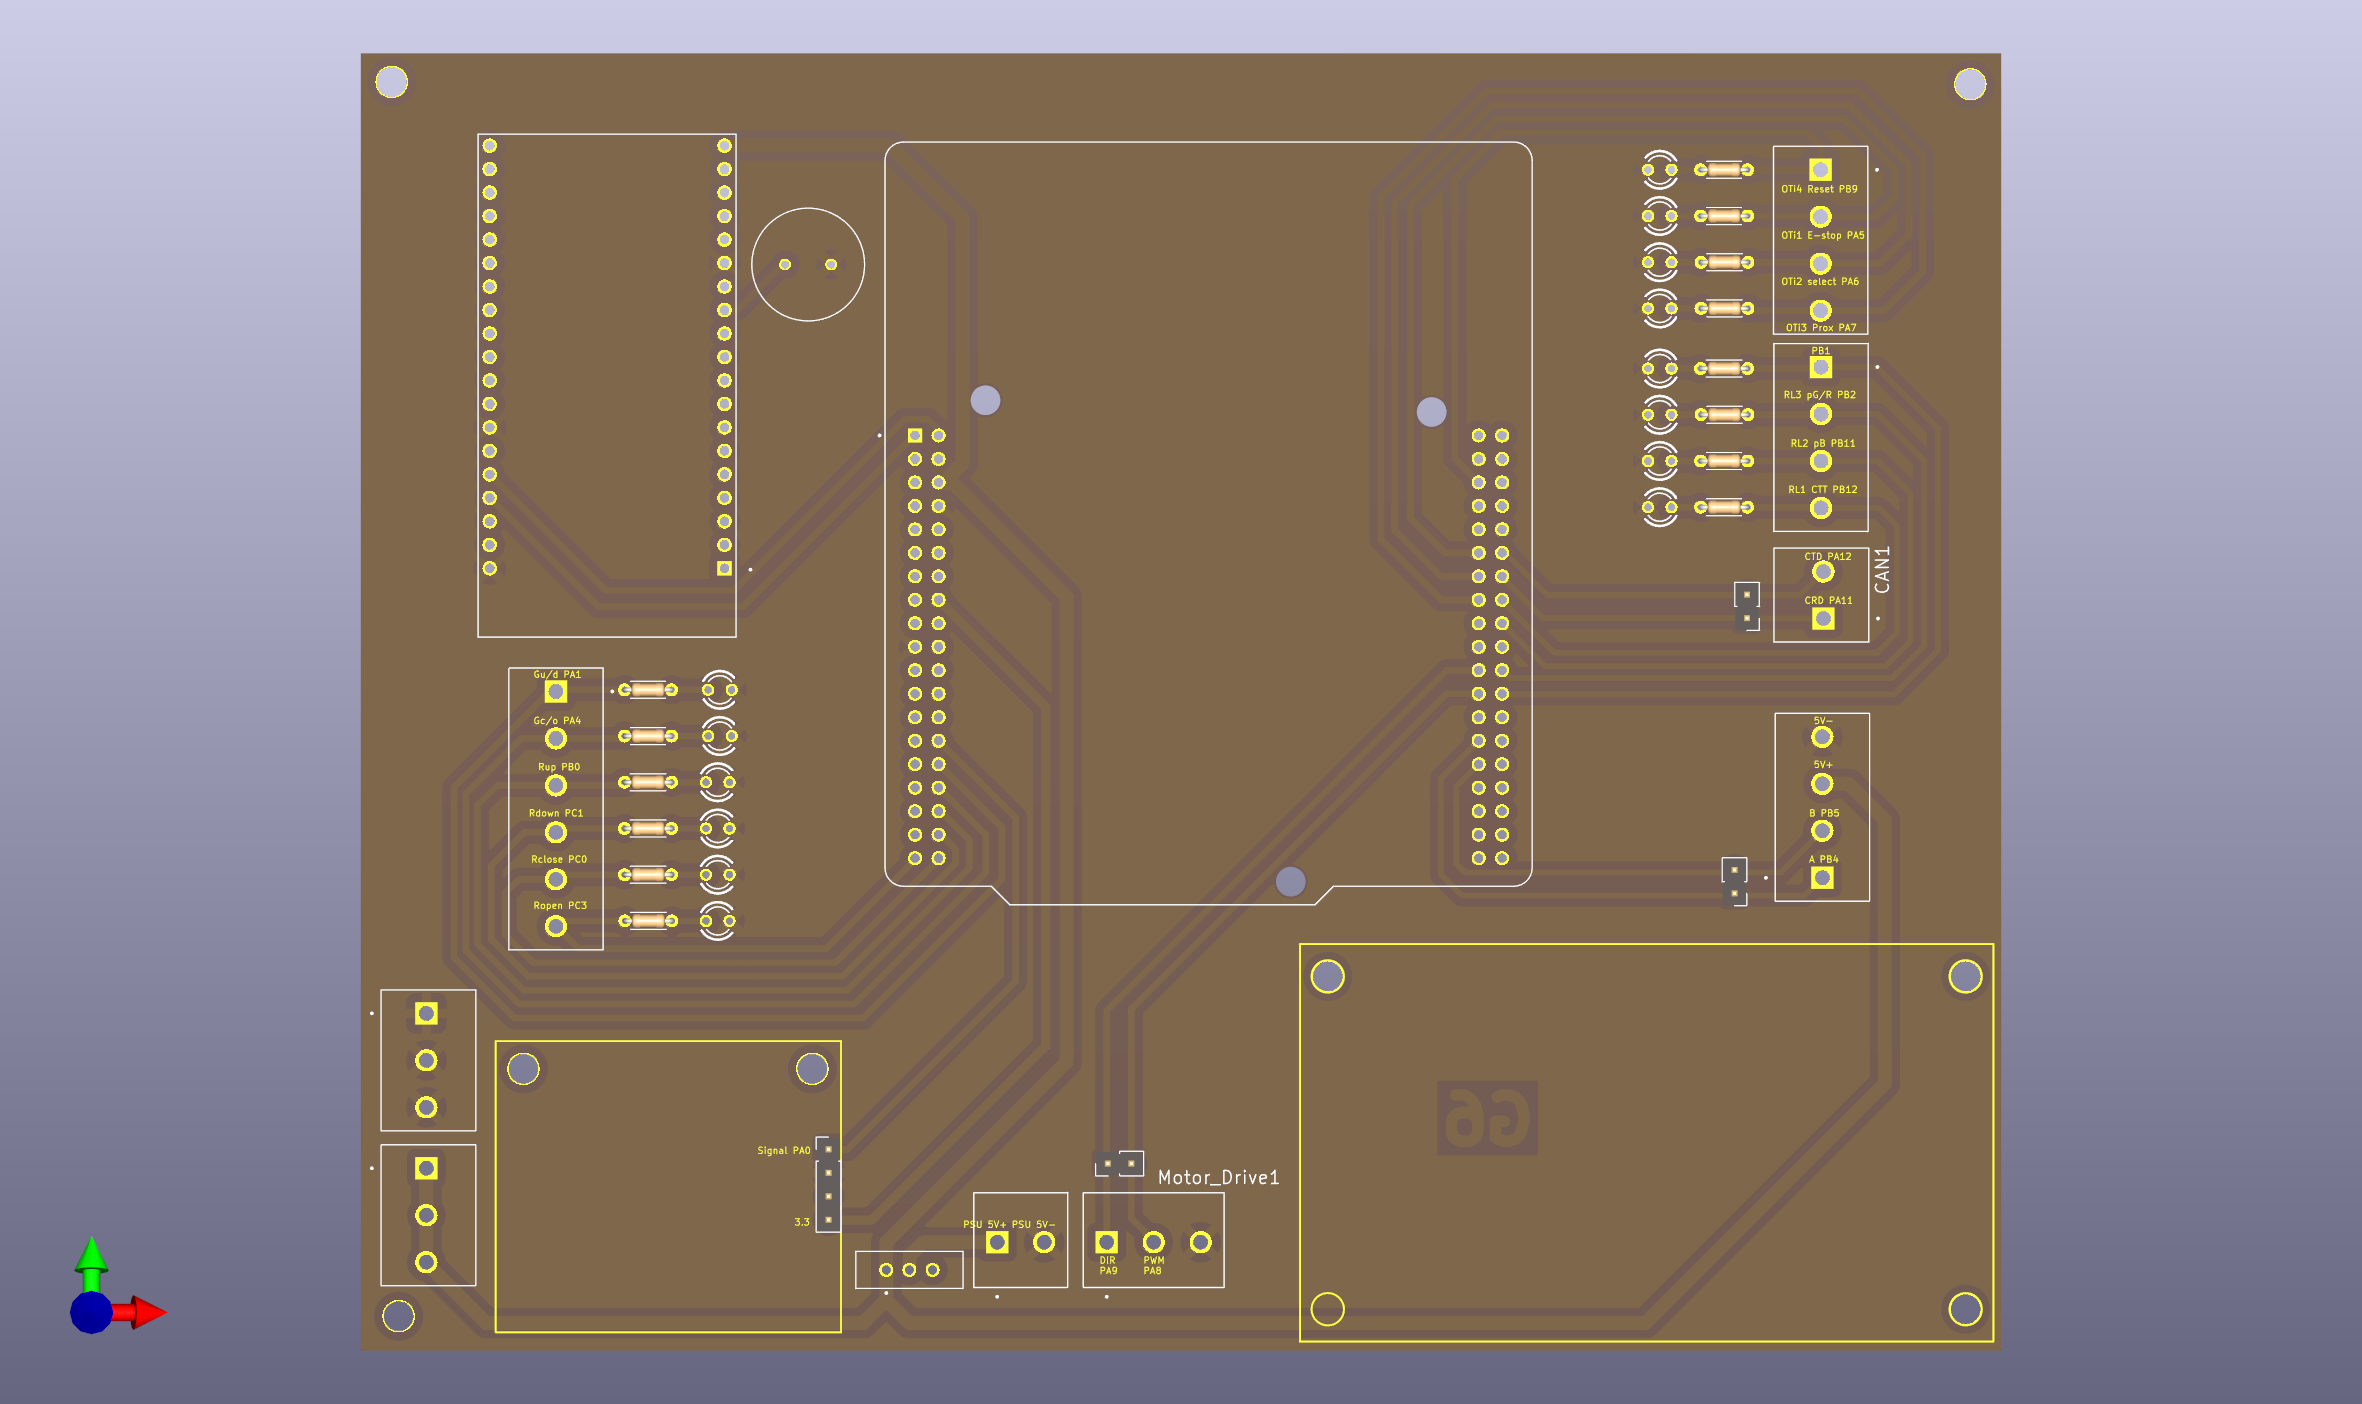
\includegraphics[width=\textwidth]{fig_pcb_3d}
        \caption{PCB 3D Render}
        \label{fig:pcb_3d}
    \end{subfigure}
    \caption{การออกแบบ PCB สำหรับระบบควบคุม
             รวม STM32, ESP32, Optocoupler และ Relay ไว้บน Board เดียว}
    \label{fig:pcb_design}
\end{figure}

% -----------------------------------------------------------------------
\subsection{STM32 Pin Assignment}
\label{subsec:pin_assignment}

Pin Assignment ทั้งหมดกำหนดใน STM32CubeMX และล็อกไว้ใน
\texttt{.ioc} file เพื่อป้องกันการเปลี่ยนแปลงโดยไม่ตั้งใจ
เมื่อ Regenerate Code

% -----------------------------------------------------------------------
% รูปที่: STM32CubeMX Pin Configuration
% ชื่อไฟล์แนะนำ: fig_cubemx_pinout.png
% เนื้อหา: Screenshot จาก STM32CubeMX แสดง Pin layout ของ STM32G474RE
%          ในมุมมอง Pinout View พร้อม color coding ตาม peripheral
%          (TIM=เขียว, UART=ส้ม, GPIO=เหลือง, ADC=ม่วง, CAN=ฟ้า)
% -----------------------------------------------------------------------
\begin{figure}[H]
    \centering
    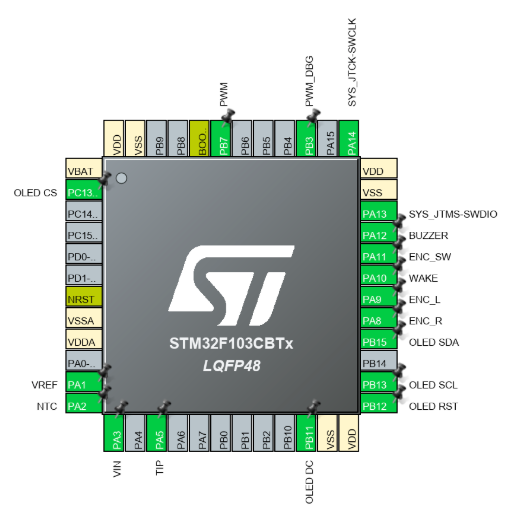
\includegraphics[width=0.75\textwidth]{fig_cubemx_pinout}
    \caption{STM32G474RE Pin Configuration จาก STM32CubeMX
             แสดง Peripheral Assignment ทั้งหมดของระบบ}
    \label{fig:cubemx_pinout}
\end{figure}

ข้อสังเกตสำคัญด้าน GPIO Configuration:

\begin{itemize}
  \item \textbf{Proximity Sensor (PB9):} ตั้งค่าเป็น
        \texttt{GPIO\_PULLUP} เนื่องจากใช้ Open-Collector
        Optocoupler ซึ่ง Active Condition คือ
        \texttt{GPIO\_PIN\_SET} (transistor หยุดนำกระแส
        pin ลอยขึ้น 3.3\,V ผ่าน Internal Pull-up)
        การตั้งค่าเป็น \texttt{GPIO\_PULLDOWN}
        จะทำให้ MCU ตรวจจับสัญญาณไม่ได้เลย
  \item \textbf{Reed Switches (PB0, PC0, PC1, PC3):}
        ตั้งค่าเป็น \texttt{GPIO\_PULLDOWN}
        เนื่องจาก Reed Switch ต่อระหว่าง Pin กับ VCC
        Active Condition คือ \texttt{GPIO\_PIN\_SET}
  \item \textbf{E-Stop (PA5):} ตั้งค่าเป็น
        \texttt{GPIO\_PULLUP} สวิตช์ต่อแบบ NC
        Active Condition คือ \texttt{GPIO\_PIN\_RESET}
        (สวิตช์กด ตัดวงจร pin ถูก Pull-up ขึ้น HIGH)
\end{itemize}

\begin{table}[H]
  \centering
  \caption{STM32G474RE Pin Assignment (จาก CubeMX IOC)}
  \label{tab:pin_assignment}
  \small
  \begin{tabular}{p{1.0cm} p{2.7cm} p{2.3cm} p{3.5cm} p{5.5cm}}
    \toprule
    Pin & GPIO Label & Signal & Mode & Config \\
    \midrule
    \multicolumn{5}{l}{\textit{Motor Control}} \\
    PA8 & Motor\_PWM        & TIM1\_CH1   & PWM Output        & AF, 19.6\,kHz, ARR=50 \\
    PA9 & Motor\_Direction  & GPIO Output & Push-Pull         & -- \\
    \midrule
    \multicolumn{5}{l}{\textit{Encoder (QEI)}} \\
    PB4 & --                & TIM3\_CH1   & Encoder Interface & NOPULL \\
    PB5 & --                & TIM3\_CH2   & Encoder Interface & NOPULL \\
    \midrule
    \multicolumn{5}{l}{\textit{Communication}} \\
    PA2  & LPUART1\_TX & LPUART1\_TX & Async UART & 230400\,bps, 8E1 \\
    PA3  & LPUART1\_RX & LPUART1\_RX & Async UART & 230400\,bps, 8E1 \\
    PC10 & --          & USART3\_TX  & Async UART & 115200\,bps, 8N1 \\
    PC11 & --          & USART3\_RX  & Async UART & 115200\,bps, 8N1 \\
    PA11 & --          & FDCAN1\_RX  & CAN Bus    & 500\,kbps classic CAN \\
    PA12 & --          & FDCAN1\_TX  & CAN Bus    & 500\,kbps classic CAN \\
    \midrule
    \multicolumn{5}{l}{\textit{Safety \& Control Input}} \\
    PA5 & E-Stop          & GPIO Input & PULLUP & Active HIGH \\
    PA6 & Selected\_Mode  & GPIO Input & PULLUP & Active LOW \\
    PA7 & Reset\_Btn      & GPIO Input & PULLUP & Active LOW \\
    PB9 & Proximity\_Sensor & GPIO Input & PULLUP & Active HIGH (open-collector) \\
    \midrule
    \multicolumn{5}{l}{\textit{Relay Output}} \\
    PB12 & Relay\_MotorPower & GPIO Output & Push-Pull & Motor Power Contactor \\
    PB11 & Relay\_Sysmode   & GPIO Output  & Push-Pull & Mode Pilot Lamp \\
    PB2  & Relay\_SysStatus & GPIO Output  & Push-Pull & Status Pilot Lamp \\
    \midrule
    \multicolumn{5}{l}{\textit{Gripper Output}} \\
    PA1 & Gripper\_Up   & GPIO Output & Push-Pull & Relay: Arm Up \\
    PA4 & Gripper\_Down & GPIO Output & Push-Pull & Relay: Arm Down \\
    \midrule
    \multicolumn{5}{l}{\textit{Reed Switch Input (Position Feedback)}} \\
    PB0 & Reed\_Up    & GPIO Input & PULLDOWN & Gripper Arm Up confirmed \\
    PC0 & Reed\_Close & GPIO Input & PULLDOWN & Claw Close confirmed \\
    PC1 & Reed\_Down  & GPIO Input & PULLDOWN & Gripper Arm Down confirmed \\
    PC3 & Reed\_Open  & GPIO Input & PULLDOWN & Claw Open confirmed \\
    \midrule
    \multicolumn{5}{l}{\textit{Analog Input}} \\
    PA0 & Current\_Sensor & ADC1\_IN1 & Analog DMA & WCS1800, DMA1\_Ch1, Continuous \\
    \bottomrule
  \end{tabular}
\end{table}

\subsection{การระบุระบบ (System Identification)}
\label{subsec:sysid}

การระบุระบบแบ่งออกเป็นสองขั้นตอนตามลำดับ ได้แก่
การวัดพารามิเตอร์ทางไฟฟ้าโดยตรงด้วย Locked Rotor Test
และการประมาณพารามิเตอร์เชิงกลด้วย Grey-box Parameter Estimation
โดยใช้ Chirp Signal เป็น Training Data
แนวทางนี้เลือกใช้เนื่องจากพารามิเตอร์ทางไฟฟ้า ($R_a$, $L_a$)
สามารถวัดได้โดยตรงจากวงจรเมื่อ Back-EMF = 0
ในขณะที่พารามิเตอร์เชิงกล ($J$, $B$, $\eta$, $K_t$, $K_b$)
ต้องอาศัยการสังเกตพฤติกรรมของระบบขณะหมุนจริง
ภายหลังการประมาณค่าพารามิเตอร์ แบบจำลองที่ได้รับการตรวจสอบ
ความถูกต้อง (Cross-Validation) ด้วยข้อมูล 2 ประเภทที่ไม่ได้ใช้
ในการ Training ได้แก่ Step Input และ Stair-Step Input
เพื่อยืนยันว่าแบบจำลองสามารถทำนายการตอบสนองได้ถูกต้อง
ทั้งในสภาวะ Transient และ Steady-State ที่แรงดันหลายระดับ

% -----------------------------------------------------------------------
\subsubsection{Locked Rotor Test: วัด $R_a$ และ $L_a$}
% -----------------------------------------------------------------------

\paragraph{หลักการและ Setup}

เมื่อล็อกเพลามอเตอร์ไม่ให้หมุน ($\omega = 0$)
Back-EMF จะมีค่าเป็นศูนย์ ($e_b = K_b\omega = 0$)
วงจรจึงลดรูปลงเหลือเพียง RL Series Circuit ดังแสดงใน\cref{fig:locked_rotor_setup}
การป้อน Step Voltage $V_{in}$ แล้ววัดแรงดันตกคร่อม Shunt Resistor $R_{sh}$
จึงเพียงพอสำหรับคำนวณทั้ง $R_a$ และ $L_a$
โดยตรงจาก KVL ของวงจร RL ตามที่อธิบายใน\cref{subsec:matlab_sysid}

\begin{equation}
    V_{in}(t) = (R_a + R_{sh})\,i(t) + L_a\,\frac{di(t)}{dt}
    \label{eq:kvl_locked}
\end{equation}

% -----------------------------------------------------------------------
% รูปที่: Locked Rotor Test — วงจรและ Oscilloscope Setup
% ชื่อไฟล์แนะนำ: fig_locked_rotor_setup.png
% เนื้อหา: วงจร RL Series แสดง V_in, R_sh, มอเตอร์ (R_a, L_a)
%          และ Oscilloscope วัดคร่อม R_sh พร้อม Probe
%          (นำจาก Slide Progress Update 2 หน้า 19 ได้เลย)
% -----------------------------------------------------------------------
\begin{figure}[H]
    \centering
    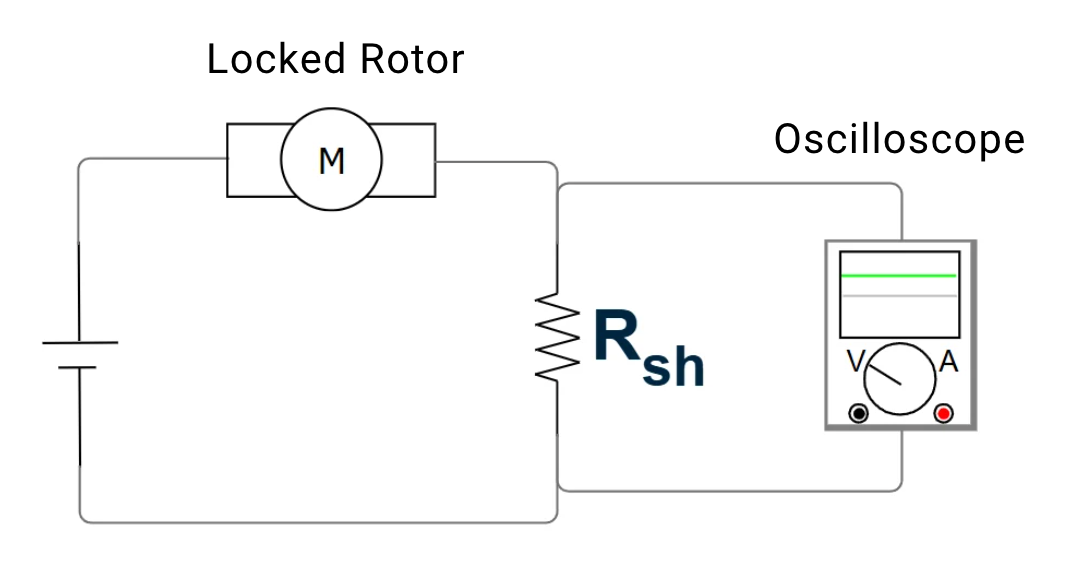
\includegraphics[width=0.75\textwidth]{fig_locked_rotor_setup}
    \caption{วงจรทดสอบ Locked Rotor Test แสดงการต่อ Shunt Resistor
             อนุกรมกับมอเตอร์เพื่อวัดกระแสทางอ้อมผ่าน Oscilloscope}
    \label{fig:locked_rotor_setup}
\end{figure}

\paragraph{การเลือก $R_{sh} = 0.1\,\Omega$}

การเลือกค่า $R_{sh}$ ต้องสอดคล้องเงื่อนไขสองข้อพร้อมกัน

\textbf{เงื่อนไขที่ 1 --- ไม่รบกวนวงจร:}
$R_{sh}$ ต้องเล็กกว่า $R_a$ มาก
เพื่อไม่ให้แรงดันตกคร่อมที่เพิ่มขึ้นเปลี่ยนพฤติกรรมของวงจร
โดยกำหนดเกณฑ์ที่ 10\%

\begin{equation}
    \frac{R_{sh}}{R_a} < 0.10
    \quad\Rightarrow\quad
    R_{sh} < 0.10 \times 1.453 = 0.1453\,\Omega
    \label{eq:rsh_cond1}
\end{equation}

\textbf{เงื่อนไขที่ 2 --- ทนกำลังไฟได้:}
กระแส Stall สูงสุดประมาณได้จาก $I_{stall} \approx V_{in}/R_a$
กำลังที่ $R_{sh}$ ต้องรับที่ $V_{in} = 12$\,V คือ

\begin{equation}
    P_{sh} = I_{stall}^2\,R_{sh}
           = \left(\frac{12}{1.453}\right)^2 \times 0.1
           = (8.26)^2 \times 0.1
           = 0.682\,\text{W}
    \label{eq:rsh_power}
\end{equation}

เลือก $R_{sh} = 0.1\,\Omega$ ขนาด 50\,W ซึ่งตอบสนองทั้งสองเงื่อนไข
และมีขนาดมาตรฐานหาซื้อได้ทั่วไป
ตรวจสอบสัดส่วน

\begin{equation}
    \frac{R_{sh}}{R_a} = \frac{0.1}{1.453} = 6.9\% < 10\%
    \quad\checkmark
    \label{eq:rsh_ratio}
\end{equation}

\paragraph{การหาสมการคำนวณพารามิเตอร์}

เมื่อระบบเข้าสู่ Steady State ($di/dt = 0$)
กระแสในวงจรคือ $i_{ss} = V_{sh,ss}/R_{sh}$
แทนลงใน\cref{eq:kvl_locked} ได้

\begin{equation}
    V_{in} = i_{ss}(R_a + R_{sh})
    \quad\Rightarrow\quad
    R_a = R_{sh}\!\left(\frac{V_{in}}{V_{sh,ss}} - 1\right)
    \label{eq:calc_Ra_ch3}
\end{equation}

การตอบสนองของกระแสเป็น First-order Exponential
ค่าคงที่เวลา $\tau = L_a/(R_a + R_{sh})$
ซึ่งวัดได้จาก Oscilloscope ที่จุด 63.2\% ของ $V_{sh,ss}$
จัดรูปใหม่ได้

\begin{equation}
    L_a = R_{sh}\!\left(\tau\,\frac{V_{in}}{V_{sh,ss}}\right)
    \label{eq:calc_La_ch3}
\end{equation}

% \cref{eq:calc_Ra_ch3,eq:calc_La_ch3} อ้างอิงมาจาก\cref{eq:calc_Ra,eq:calc_La}
% ในบทที่~2 โดยใช้ $V_{sh,ss}$ ซึ่งวัดได้โดยตรงจาก Oscilloscope Waveform
% ดังแสดงใน\cref{fig:locked_rotor_scope}

% -----------------------------------------------------------------------
% รูปที่: Oscilloscope Waveform จาก Locked Rotor Test
% ชื่อไฟล์แนะนำ: fig_locked_rotor_scope.png
% เนื้อหา: Oscilloscope screenshot แสดง waveform ของ V_sh
%          ระบุจุด V_sh,ss (Steady-State) และจุด 63.2% สำหรับอ่านค่า tau
%          พร้อม annotation แสดงระยะเวลา tau บนแกน X
%          (มีรูปนี้อยู่ใน Progress Report 2 แล้ว ใช้ได้เลย)
% -----------------------------------------------------------------------
\begin{figure}[H]
    \centering
    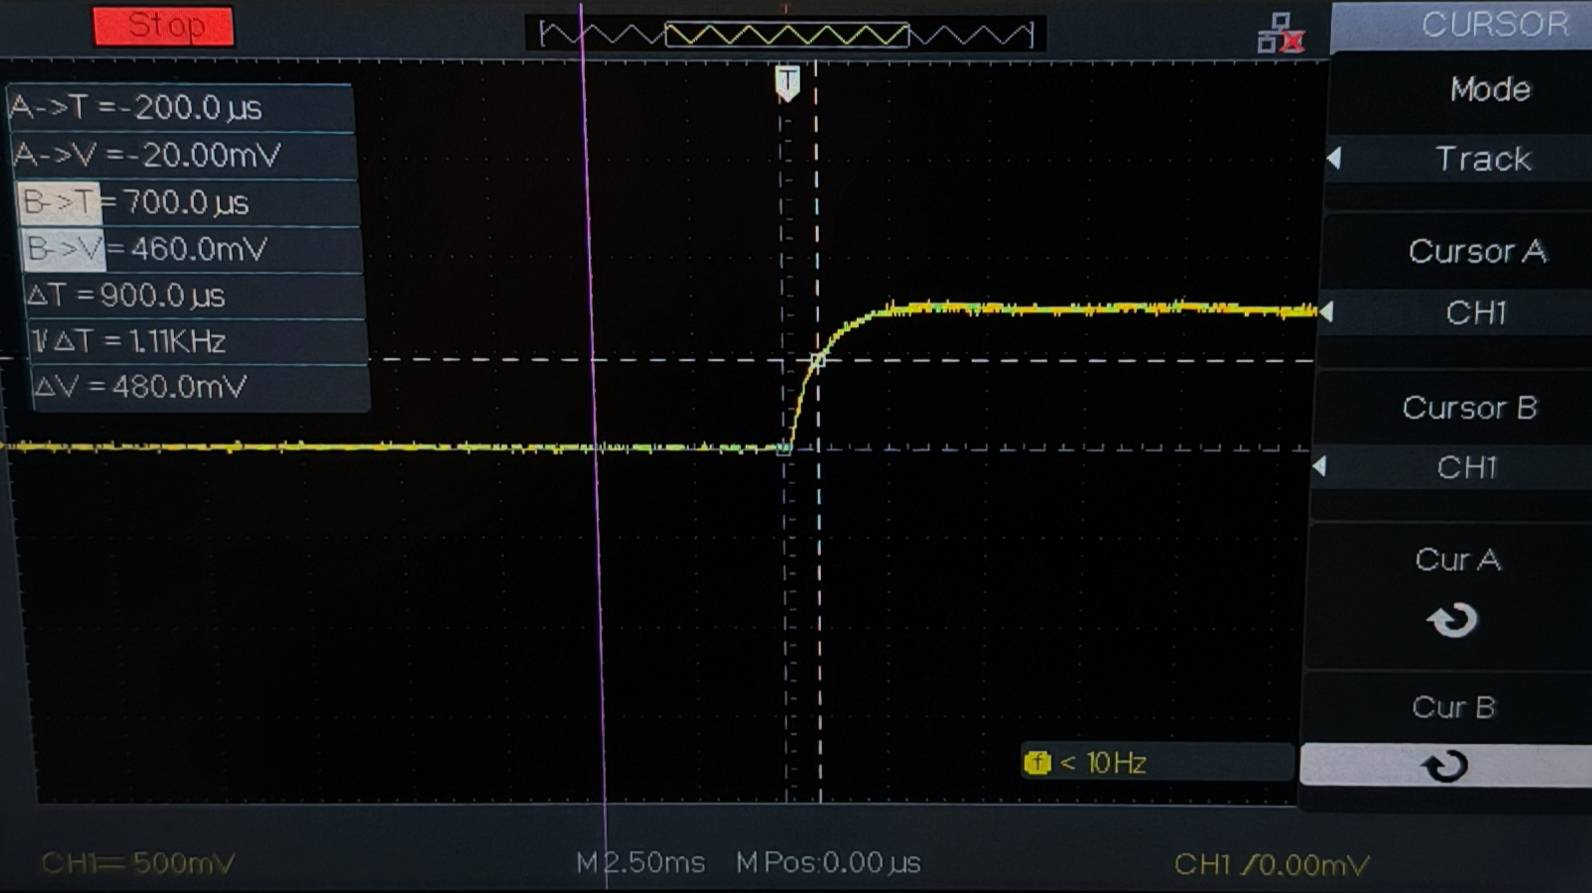
\includegraphics[width=0.70\textwidth]{fig_locked_rotor_scope}
    \caption{Oscilloscope Waveform จาก Locked Rotor Test ที่ $V_{in} = 12$\,V
             แสดงแรงดัน $V_{sh}$ ที่ไต่ระดับแบบ First-order Exponential
             พร้อมจุดอ่านค่า $V_{sh,ss}$ และ $\tau$}
    \label{fig:locked_rotor_scope}
\end{figure}

\paragraph{การเลือกแรงดันทดสอบและการวิเคราะห์ความสม่ำเสมอ}

ทดสอบที่แรงดัน 3 ระดับ ($V_{in} = 6$, $9$, $12$\,V)
โดยแต่ละระดับทำซ้ำ 3 ครั้งเพื่อประเมิน Statistical Consistency

\begin{table}[H]
  \centering
  \caption{ผลการวัด $R_a$ และ $L_a$ จาก Locked Rotor Test ทั้ง 3 แรงดัน}
  \label{tab:locked_rotor_all}
  \begin{tabular}{ccccc}
    \toprule
    $V_{in}$ (V) & $\bar{R}_a$ ($\Omega$) & $\sigma_{R_a}$ ($\Omega$)
                 & $\bar{L}_a$ (H)        & $\sigma_{L_a}$ (H) \\
    \midrule
    6  & 1.7300 & 0.0374 & 0.001490 & 0.000062 \\
    9  & 1.5398 & 0.0604 & 0.001473 & 0.000095 \\
    12 & \textbf{1.4534} & 0.0523 & \textbf{0.001448} & 0.000055 \\
    \bottomrule
  \end{tabular}
\end{table}

จากตารางพบว่าค่า $\bar{R}_a$ มีแนวโน้มลดลงเมื่อแรงดันเพิ่มขึ้น
สาเหตุหลักมาจากสองปัจจัย ได้แก่

\begin{itemize}
  \item \textbf{Contact Resistance:}
        ที่ $V_{in}$ ต่ำ กระแสที่ไหลผ่าน Brush Contact มีค่าน้อย
        ทำให้ความต้านทานสัมผัสของแปรงถ่านมีสัดส่วนสูงกว่าในค่า $R_a$ รวม
        เมื่อแรงดันสูงขึ้น กระแสเพิ่มขึ้น สัดส่วนของ Contact Resistance ลดลง
  \item \textbf{Signal-to-Noise Ratio:}
        ที่ $V_{in} = 6$\,V แรงดัน $V_{sh,ss} \approx 0.37$\,V
        ซึ่งมีขนาดใกล้เคียงกับ Noise Floor ของ Oscilloscope
        ทำให้ Error ในการอ่านค่า $\tau$ และ $V_{sh,ss}$ สูงกว่า
        สะท้อนใน $\sigma_{R_a} = 0.0374\,\Omega$ ที่ต่ำผิดปกติ
\end{itemize}

เลือกใช้ผลจาก $V_{in} = 12$\,V เป็นค่าอ้างอิงด้วยสองเหตุผล ได้แก่
ใกล้เคียงแรงดันใช้งานจริง 24\,V มากที่สุดในชุดที่ทดสอบ
ทำให้สภาวะ Brush Contact สอดคล้องกับการทำงานจริง
และ $\sigma_{R_a} = 0.0523\,\Omega$ ต่ำที่สุดในสามแรงดัน
ยืนยันความสม่ำเสมอของการวัด
ทั้งนี้ไม่ทดสอบที่ 24\,V เนื่องจากเพลาจะหมุนแรงเกินไปและอาจก่อให้เกิดอันตรายได้

% -----------------------------------------------------------------------
\subsubsection{Chirp Excitation และ Grey-box Parameter Estimation}
% -----------------------------------------------------------------------

\paragraph{เหตุผลในการเลือก Chirp Signal}

พารามิเตอร์เชิงกล ($J$, $B$, $\eta$, $K_t$, $K_b$)
ไม่สามารถวัดโดยตรงได้จากวงจร
จำเป็นต้องสังเกตพฤติกรรมของระบบขณะหมุนจริงภายใต้ Input ที่ครอบคลุม
Frequency Content ของ Slow Dynamics ที่ต้องการระบุ
Chirp Signal (Linear Frequency Sweep) ถูกเลือกเนื่องจาก

\begin{itemize}
  \item \textbf{Persistent Excitation:}
        Chirp ที่ Sweep จาก $f_1$ ถึง $f_2$ การันตีว่าทุก Frequency
        ในช่วงดังกล่าวได้รับการกระตุ้น ต่างจาก Step Signal
        ที่มี Spectral Energy กระจุกที่ DC และลดลงตาม $1/f$
  \item \textbf{ครอบคลุม Mechanical Bandwidth:}
        ย่านความถี่ 0.1--2.0\,Hz ครอบคลุม Slow Dynamics ของ Inertia
        และ Viscous Damping เมื่อเทียบกับ Mechanical Bandwidth
        ของระบบที่คำนวณได้จากพารามิเตอร์ทางไฟฟ้า

        \begin{equation}
            f_{mech} = \frac{1}{2\pi}
                       \sqrt{\frac{R_a B + K_b K_t N^2}{L_a J}}
                     = \frac{\sqrt{8136}}{2\pi}
                     \approx 14.4\,\text{Hz}
            \label{eq:f_mech}
        \end{equation}

        ย่าน 0.1--2.0\,Hz จึงอยู่ต่ำกว่า $f_{mech}$ อย่างมีนัยสำคัญ
        ทำให้ Dynamic ที่วัดได้สะท้อน Inertia และ Damping โดยตรง
        โดยไม่ปะปนกับ Electrical Pole ที่ $R_a/L_a \approx 1004$\,rad/s
\end{itemize}

\paragraph{Preprocessing และ Filtering}

ข้อมูลดิบกรองด้วย Butterworth Low-pass Filter Order~4
ที่ $f_c = 10$\,Hz ด้วยคำสั่ง \texttt{filtfilt} ของ MATLAB
(หลักการ Zero-Phase Filtering อธิบายไว้ใน\cref{subsec:filtfilt})
เลือก $f_c = 10$\,Hz เนื่องจาก

\begin{itemize}
  \item สูงกว่าย่านความถี่ Identification (0.1--2.0\,Hz) ถึง 5 เท่า
        ทำให้ Attenuation ที่ขอบบนของย่าน ($f = 2$\,Hz)
        น้อยกว่า 0.001\% ตามที่แสดงใน\cref{eq:filtfilt_mag}
        จึงไม่ลดทอน Amplitude ของ Signal ที่ต้องการ
  \item กำจัด Noise จาก PWM Switching ($f_{pwm} = 19.6$\,kHz)
        และ Quantization Noise ของ Encoder ที่ความถี่สูงได้อย่างมีประสิทธิภาพ
\end{itemize}

ความถูกต้องของการเลือก $f_c$ ซึ่งแสดงว่า Magnitude และ Phase
ของ \texttt{filtfilt} ทับกับ Raw Signal ได้อย่างสมบูรณ์
ในย่าน 0.1--2.0\,Hz และ\cref{fig:filtfilt_concept}
แสดงให้เห็นว่า \texttt{filtfilt} ไม่มี Phase Lag
ต่างจาก Causal Filter ที่มี Lag สังเกตได้ชัดเจน

\begin{figure}[H]
    \centering
    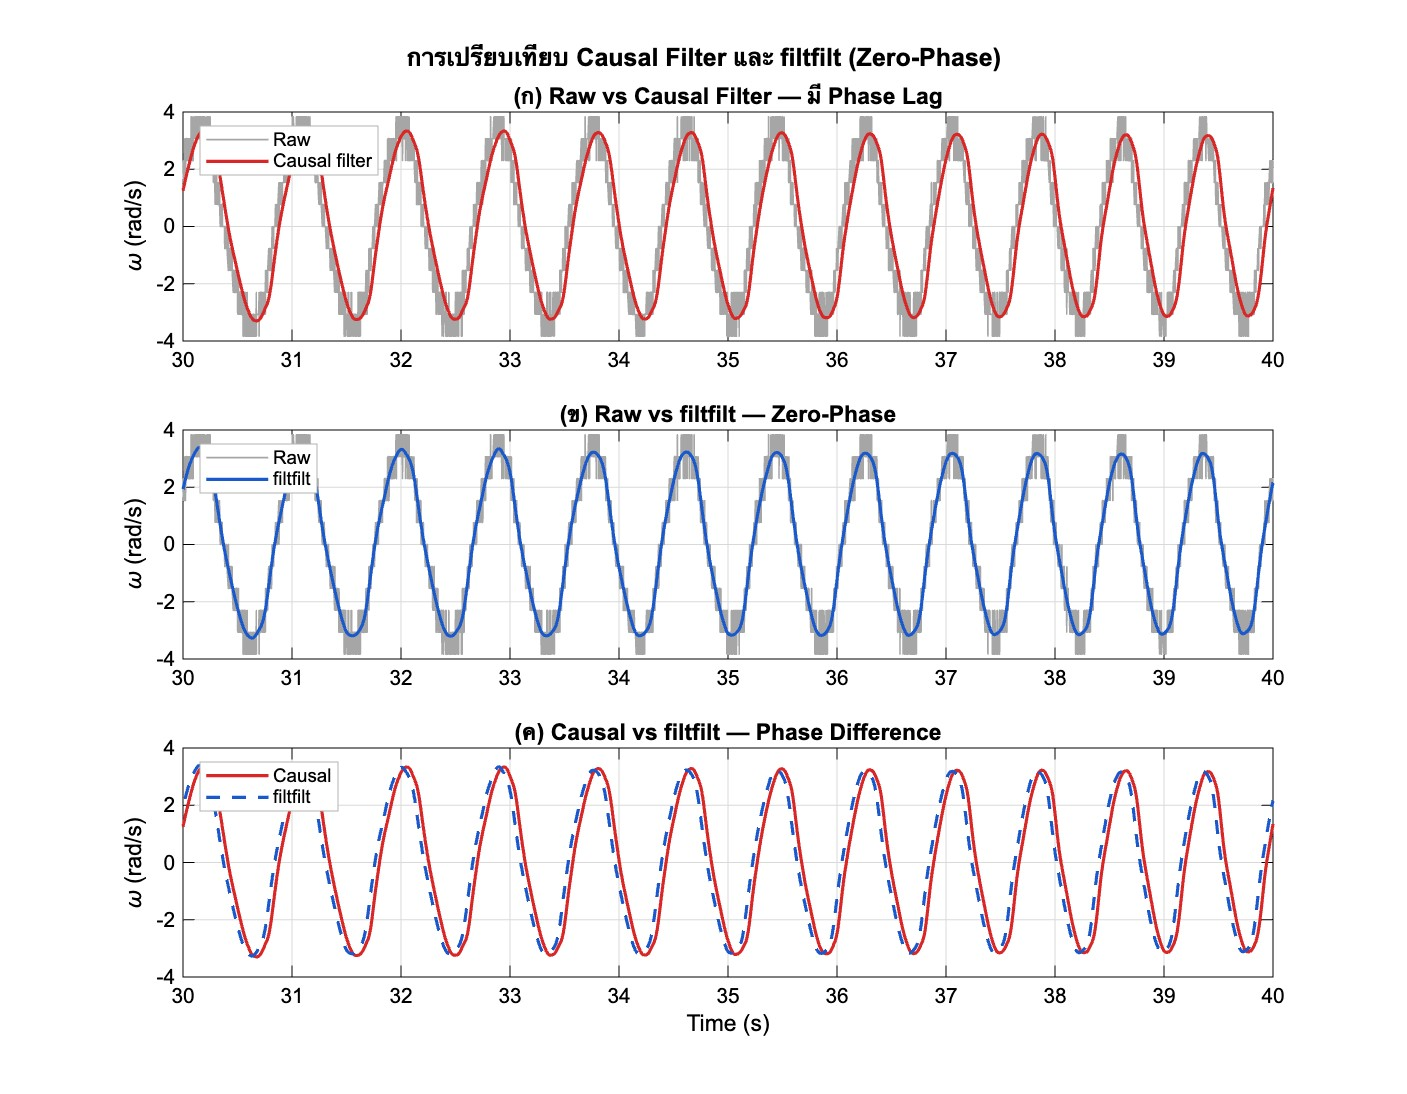
\includegraphics[width=0.90\textwidth]{fig_filfilt.jpg}
    \caption{เปรียบเทียบ Causal Filter (สีแดง) และ \texttt{filtfilt}
             (สีน้ำเงิน) ในโดเมนเวลา
             (ก)~Causal Filter มี Phase Lag สังเกตได้ชัดเจน
             (ข)~\texttt{filtfilt} ทับ Raw Signal ได้ตรงทุกจุด
             (ค)~Phase Difference ระหว่างสองวิธี}
    \label{fig:filtfilt_concept}
\end{figure}

\begin{figure}[H]
    \centering
    \begin{subfigure}[b]{0.48\textwidth}
        \centering
        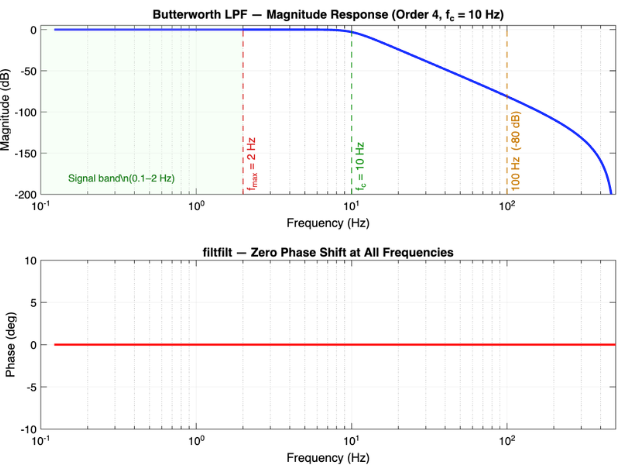
\includegraphics[width=\textwidth]{fig_butter_bode_actual}
        \caption{Magnitude Response ของ Butterworth LPF Order~4
                 ($f_c = 10$\,Hz) และ Phase Response ของ
                 \texttt{filtfilt} ที่เป็นศูนย์ในทุกความถี่}
        \label{fig:butter_bode_actual}
    \end{subfigure}
    \hfill
    \begin{subfigure}[b]{0.48\textwidth}
        \centering
        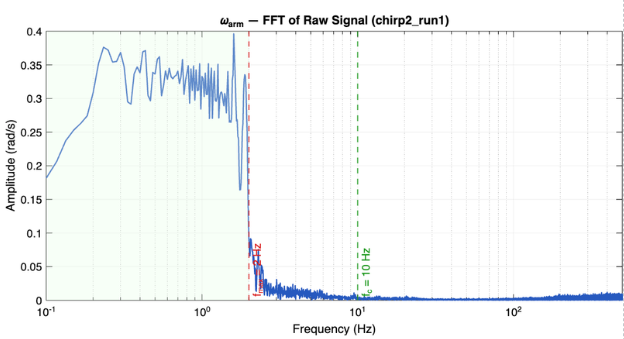
\includegraphics[width=\textwidth]{fig_fft_raw_actual}
        \caption{FFT ของ Raw Signal $\omega_{arm}$
                 จาก Chirp Run 1 (0.1--2\,Hz)
                 แสดง Signal Energy กระจุกที่ 0.1--2\,Hz
                 และ Noise Floor ที่ความถี่สูงกว่า $f_c = 10$\,Hz}
        \label{fig:fft_raw_actual}
    \end{subfigure}
    \caption{การตรวจสอบความเหมาะสมของ $f_c = 10$\,Hz
             กับข้อมูลจริงของระบบ:
             (ซ้าย) \texttt{filtfilt} ให้ Phase Shift เป็นศูนย์
             และ Attenuation ที่ 2\,Hz น้อยกว่า 0.001\%
             (ขวา) Signal Dynamics ของระบบจริงทั้งหมด
             อยู่ในย่าน 0.1--2\,Hz ห่างจาก $f_c$ ถึง 5 เท่า
             ยืนยันว่า Filter ไม่รบกวน Signal ที่ต้องการ}
    \label{fig:preprocessing_validation}
\end{figure}

ผลใน\cref{fig:preprocessing_validation} ยืนยันความเหมาะสมของการเลือก
$f_c = 10$\,Hz จากสองมุมมอง ได้แก่

\textbf{มุมมองที่ 1 --- คุณสมบัติของ Filter (กราฟซ้าย):}
Butterworth LPF Order~4 มี Magnitude Response แบน (0\,dB)
ในย่าน Passband ตลอด 0.1--2\,Hz โดยไม่มี Ripple
และ Roll-off เริ่มต้นที่ $f_c = 10$\,Hz
ที่ความถี่ 100\,Hz ซึ่งเป็นย่าน Noise
Filter ลดทอนสัญญาณได้ถึง $-80$\,dB หรือเทียบเท่า
ลดแอมพลิจูดลง 10,000 เท่า
ที่สำคัญ Phase Response ของ \texttt{filtfilt}
เป็นเส้นตรงที่ $0°$ ในทุกความถี่โดยไม่มีข้อยกเว้น
ยืนยันว่าไม่มี Phase Distortion เกิดขึ้นกับ Signal ใดๆ
ในชุดข้อมูล

\textbf{มุมมองที่ 2 --- Spectral Content ของข้อมูลจริง (กราฟขวา):}
FFT ของ $\omega_{arm}$ จาก Chirp Run 1 แสดงให้เห็นชัดว่า
Signal Energy ทั้งหมดกระจุกอยู่ในย่าน 0.1--2\,Hz
ตรงกับความถี่ของ Chirp Input ที่ป้อนเข้าระบบ
หลังจาก $f = 2$\,Hz แอมพลิจูดลดลงอย่างรวดเร็ว
และกลายเป็น Noise Floor ที่มีขนาดเล็กมาก
($< 0.01$\,rad/s) ตลอดย่าน 2--500\,Hz
ระยะห่างระหว่าง $f_{max,signal} = 2$\,Hz
และ $f_c = 10$\,Hz จึงมี Margin 5 เท่า
ซึ่งเพียงพอที่จะการันตีว่า Filter
ไม่ตัด Signal ที่มีประโยชน์ออกไปแม้แต่น้อย

\paragraph{Grey-box Estimation บน MATLAB}

การประมาณค่าพารามิเตอร์ใช้ \texttt{idgrey} + \texttt{greyest}
บน MATLAB System Identification Toolbox
โดยกำหนดโครงสร้างเมทริกซ์ $\mathbf{A}$, $\mathbf{B}$, $\mathbf{C}$
ตามสมการ State-Space ใน\cref{eq:ABCD_matrices}
แล้วปล่อยให้ $\mathbf{p} = [K_t,\; K_b,\; J,\; B,\; \eta]^\top$
เป็น Free Parameters
อัลกอริทึมใช้ Prediction Error Method (PEM)
ลดรูป Cost Function

\begin{equation}
    V_N(\mathbf{p}) = \frac{1}{N}\sum_{k=1}^{N}
                      \bigl|y(k) - \hat{y}(k\mid\mathbf{p})\bigr|^2
    \label{eq:pem_cost_ch3}
\end{equation}

\noindent ตามที่อธิบายใน\cref{subsec:matlab_sysid}
ทดสอบ 3 ย่านความถี่ $\times$ 3 runs/ย่าน = 9 Experiments รวม
ดังแสดงใน\cref{tab:chirp_config}

\begin{table}[H]
  \centering
  \caption{การตั้งค่า Chirp Signal สำหรับ Grey-box Estimation}
  \label{tab:chirp_config}
  \begin{tabular}{lccc}
    \toprule
    ย่านความถี่ & $f_{start}$ (Hz) & $f_{end}$ (Hz) & จำนวน Runs \\
    \midrule
    Low Band    & 0.1 & 0.5 & 3 \\
    Mid Band    & 0.1 & 1.0 & 3 \\
    High Band   & 0.1 & 2.0 & 3 \\
    \midrule
    \textbf{รวม} & -- & -- & \textbf{9} \\
    \bottomrule
  \end{tabular}
\end{table}

% -----------------------------------------------------------------------
% รูปที่: MATLAB Simulink Block Diagram สำหรับ Grey-box Estimation
% ชื่อไฟล์แนะนำ: fig_sysid_simulink.png
% เนื้อหา: Simulink model แสดง State-Space ของมอเตอร์
%          พร้อม Free Parameters ที่ highlight ด้วยสี
%          (นำจาก Slide Progress Update 2 หน้า 21 ได้เลย)
% -----------------------------------------------------------------------
\begin{figure}[H]
    \centering
    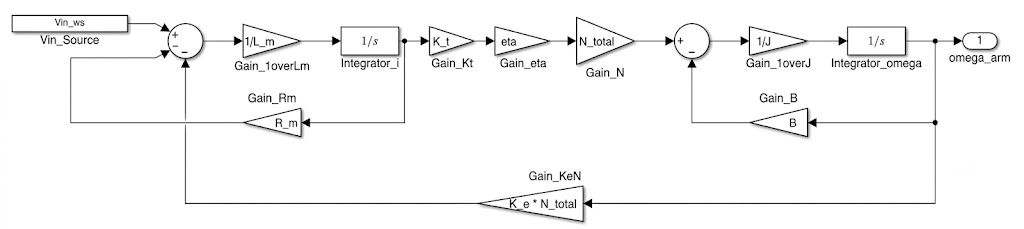
\includegraphics[width=0.90\textwidth]{fig_sysid_simulink}
    \caption{Simulink Block Diagram ของแบบจำลอง DC Motor
             ที่ใช้ใน Grey-box Parameter Estimation
             แสดง Free Parameters ที่ปรับค่าโดย \texttt{greyest}}
    \label{fig:sysid_simulink}
\end{figure}

\paragraph{Cross-Validation}

เพื่อยืนยันว่าแบบจำลองที่ได้ไม่เกิด Overfitting กับ Chirp Training Data
จึงทดสอบกับข้อมูล 2 ประเภทที่ไม่ได้ใช้ใน Training ได้แก่
Step Input (3 แรงดัน: 6, 12, 24\,V) และ Stair-Step Input
รวม 21 Runs ทั้งหมด
ผล Fit Score วัดจาก NRMSE ระหว่าง Simulated Output
กับ Measured Data แสดงใน\cref{tab:crossval_fit}
และ\cref{fig:crossval_all_runs}

\begin{table}[H]
  \centering
  \caption{ผลการ Cross-Validation ของแบบจำลองกับข้อมูลประเภทต่าง ๆ}
  \label{tab:crossval_fit}
  \begin{tabular}{llcc}
    \toprule
    ประเภทข้อมูล & แรงดัน & Fit Score (\%) & หมายเหตุ \\
    \midrule
    Chirp (Training) & 0.1--0.5\,Hz & 88.3--97.1 & -- \\
    Chirp (Training) & 0.1--1.0\,Hz & 93.9--98.1 & -- \\
    Chirp (Training) & 0.1--2.0\,Hz & 81.8--92.2 & -- \\
    \midrule
    Step (Validation) & 6\,V  & 33.6--59.8 & Static Friction dominant \\
    Step (Validation) & 12\,V & 76.7--90.8 & -- \\
    Step (Validation) & 24\,V & 84.7--95.4 & -- \\
    Stair-Step (Validation) & 24\,V & 95.2--96.6 & -- \\
    \bottomrule
  \end{tabular}
\end{table}

\begin{figure}[H]
    \centering
    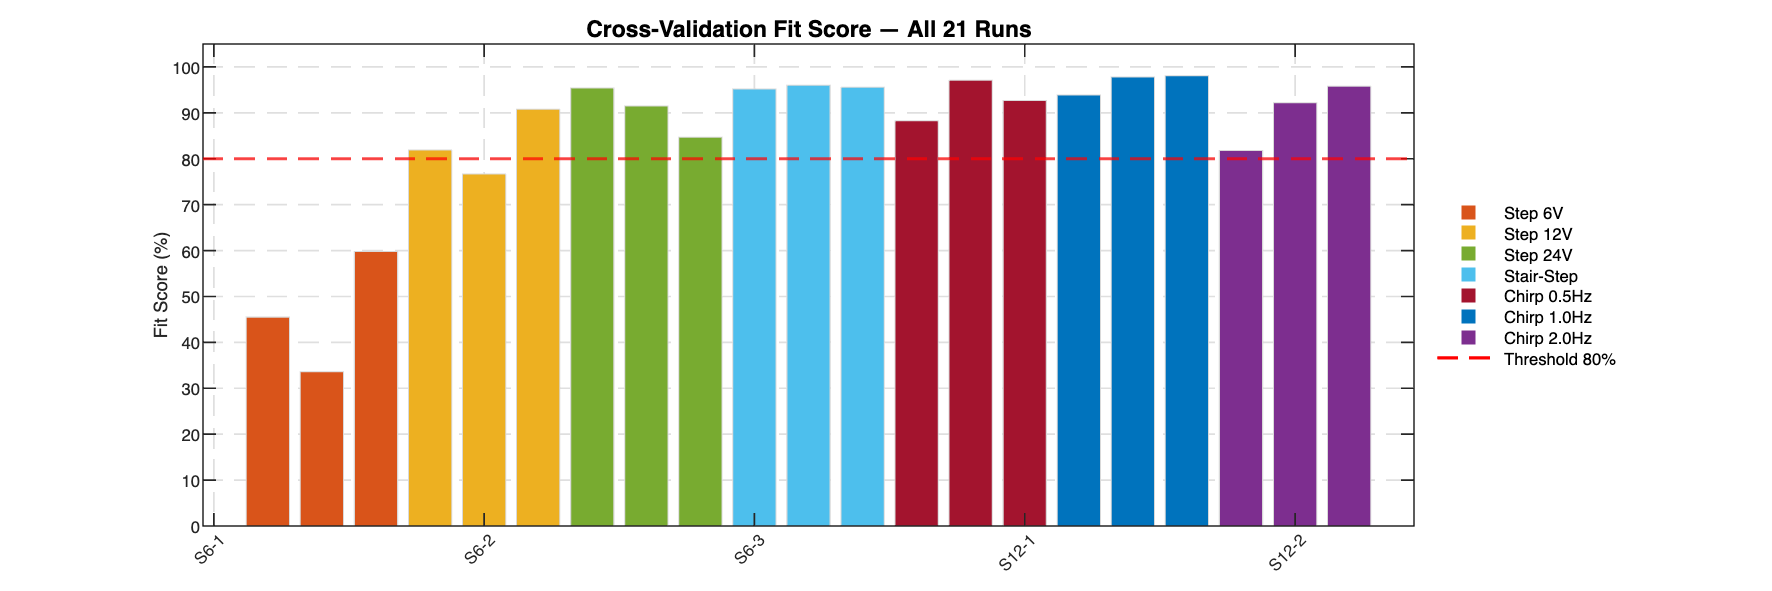
\includegraphics[width=1\textwidth]{fig_crossval_histogram}
    \caption{Cross-Validation Fit Score ทั้ง 21 Runs แสดงเป็น Histogram
             จำแนกตามประเภทข้อมูล
             เส้นประสีแดงคือเกณฑ์ขั้นต่ำที่ยอมรับได้ 80\%}
    \label{fig:crossval_histogram}
\end{figure}

\begin{figure}[H]
    \centering
    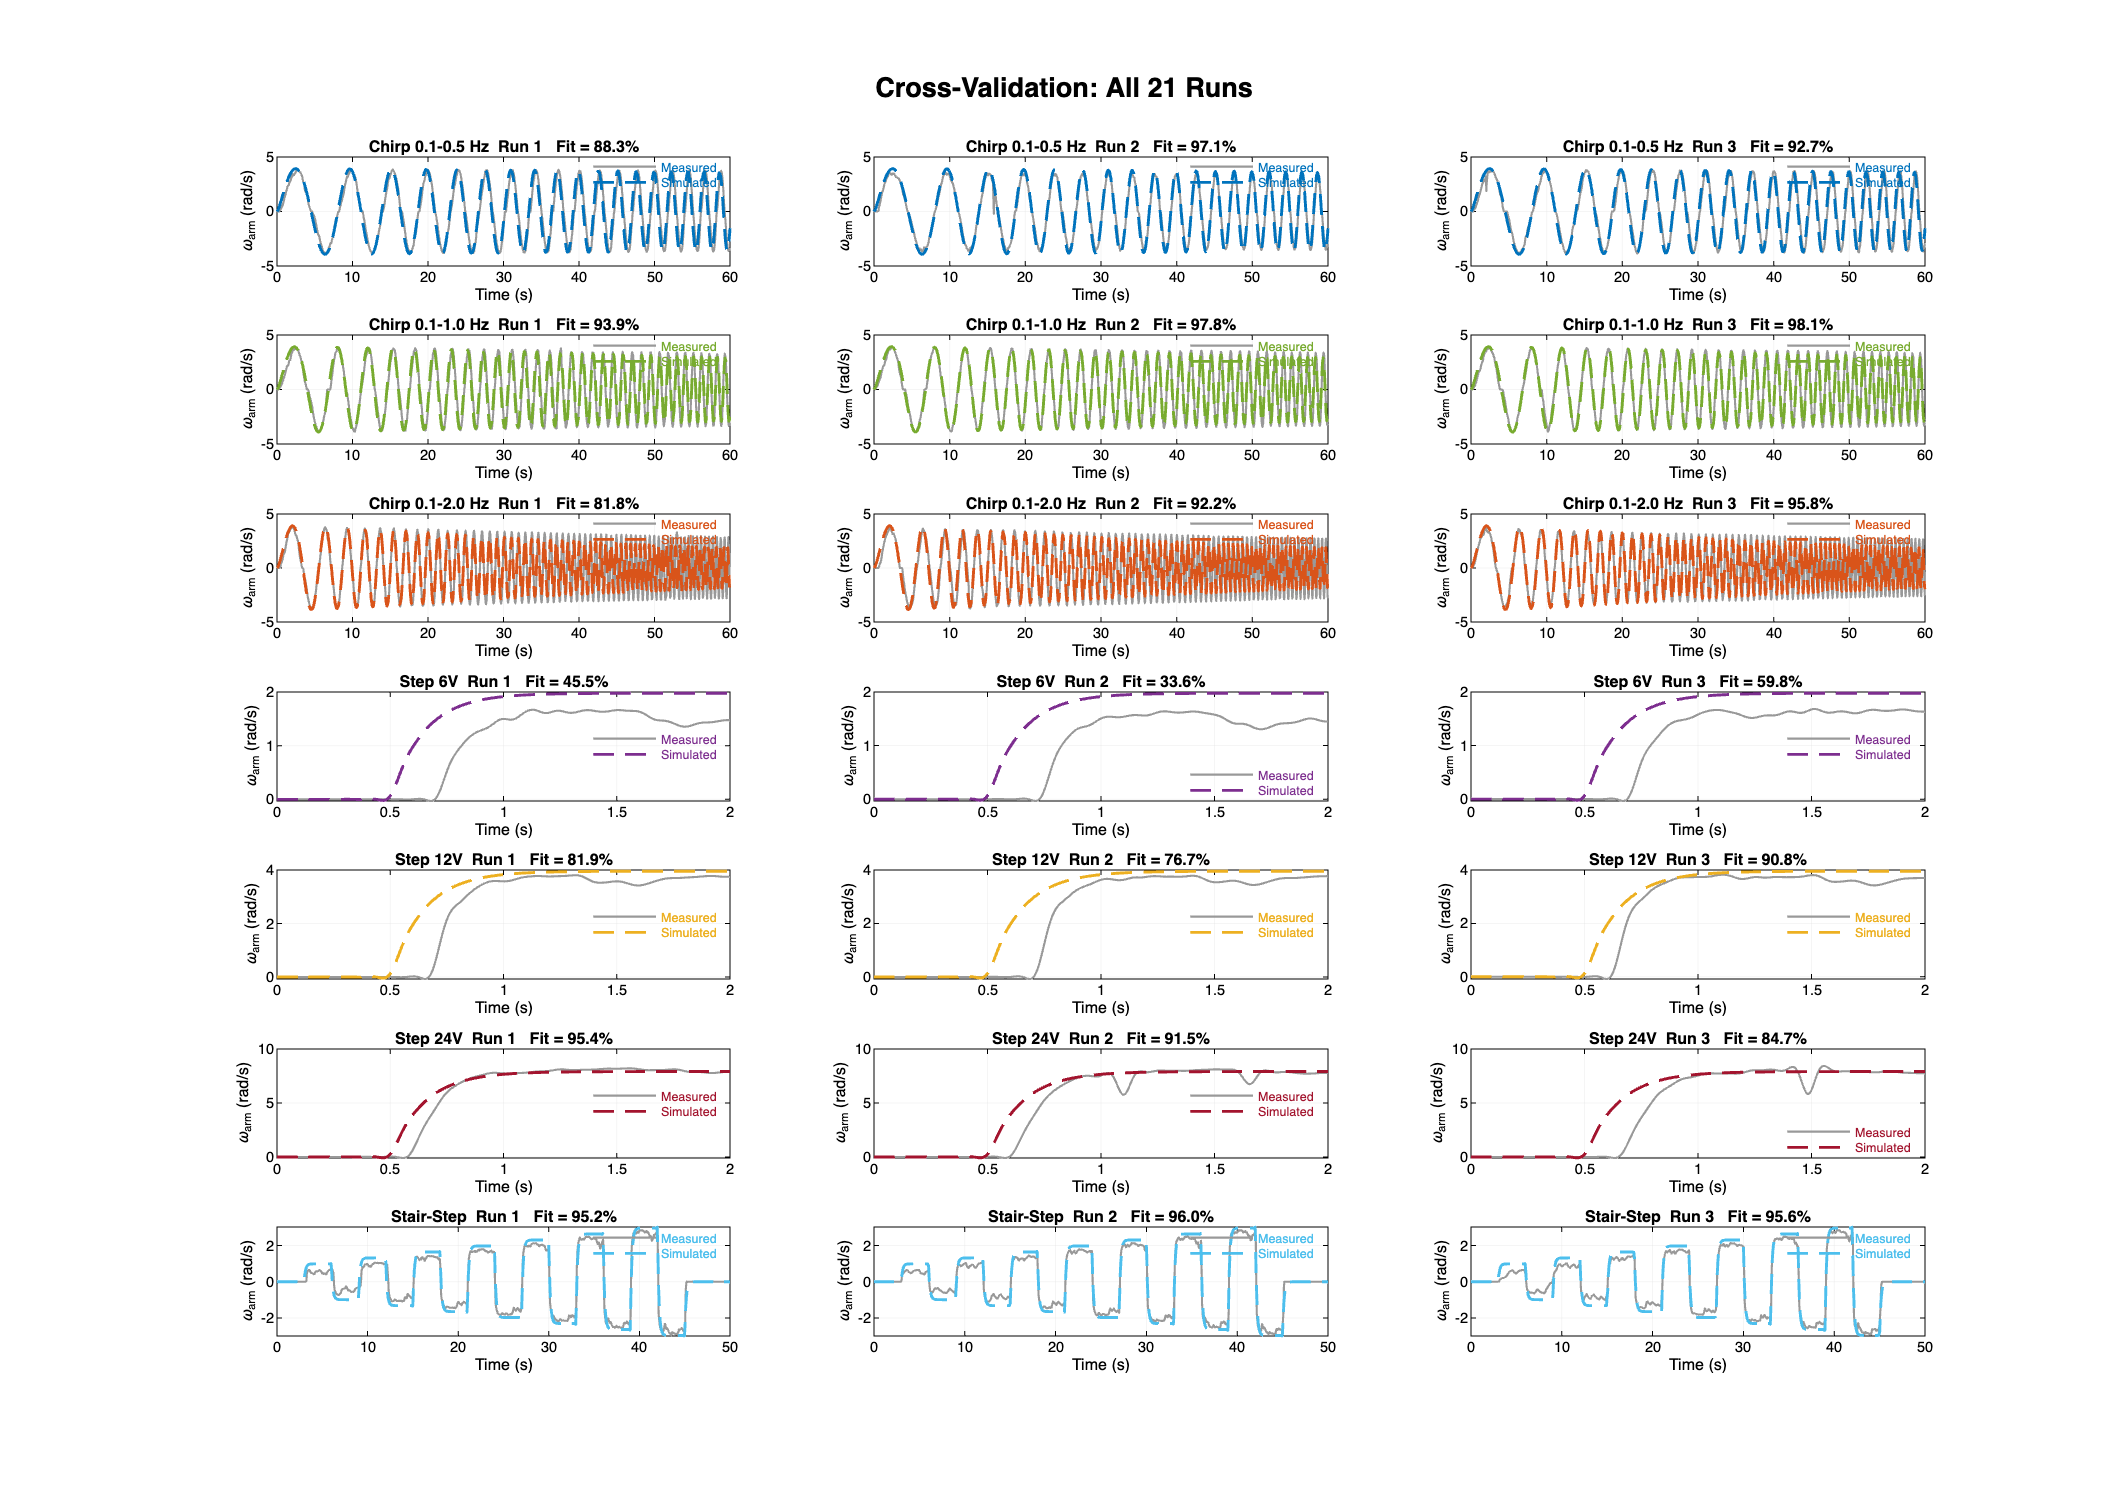
\includegraphics[width=\textwidth]{fig_crossval_all_runs}
    \caption{เปรียบเทียบ Measured (เส้นทึบ) และ Simulated (เส้นประ)
             ทั้ง 21 Runs จำแนกตามประเภท Input
             ได้แก่ Chirp 3 ย่านความถี่, Step 3 แรงดัน และ Stair-Step}
    \label{fig:crossval_all_runs}
\end{figure}

ผล Fit Score ที่ต่ำผิดปกติที่ Step 6\,V (33.6--59.8\%)
เกิดจาก Static Friction ของ Bearing และ Belt Drive
มีนัยสำคัญที่แรงดันต่ำ ในขณะที่แบบจำลองเชิงเส้น
ตาม\cref{eq:mechanical_ode} ละทิ้ง Coulomb Friction ออกไป
ตามสมมติฐานใน\cref{sec:dc_motor_model}
อย่างไรก็ตาม ที่แรงดันใช้งานจริง 24\,V
Fit Score = 84.7--95.4\% (Step) และ 95.2--96.6\% (Stair-Step)
ยืนยันว่าแบบจำลองเพียงพอสำหรับการออกแบบตัวควบคุม
ในย่านแรงดันที่ใช้งานจริง

% -----------------------------------------------------------------------
\subsubsection{ผลการระบุระบบ}
% -----------------------------------------------------------------------

\begin{table}[H]
  \centering
  \caption{พารามิเตอร์ที่ได้จาก System Identification}
  \label{tab:sysid_params}
  \begin{tabular}{llccc}
    \toprule
    พารามิเตอร์ & สัญลักษณ์ & ค่า & หน่วย & วิธีการ \\
    \midrule
    Armature Resistance & $R_a$  & 1.4534   & $\Omega$              & Locked Rotor Test \\
    Armature Inductance & $L_a$  & 0.001448 & H                     & Locked Rotor Test \\
    Back-EMF Constant   & $K_b$  & 0.04165  & V$\cdot$s/rad         & Grey-box Estimation \\
    Torque Constant     & $K_t$  & 0.04065  & N$\cdot$m/A           & Grey-box Estimation \\
    Viscous Damping     & $B$    & 0.19279  & N$\cdot$m$\cdot$s/rad & Grey-box Estimation \\
    Moment of Inertia   & $J$    & 0.72762  & kg$\cdot$m$^2$        & Grey-box Estimation \\
    Total Gear Ratio    & $N$    & 70       & --                    & $N_g \times N_b$ \\
    Efficiency          & $\eta$ & 0.836    & --                    & Grey-box Estimation \\
    \bottomrule
  \end{tabular}
\end{table}

\paragraph{การ Derive Transfer Function}

แทนค่าพารามิเตอร์จากตารางลงในสมการ State-Space
ใน\cref{eq:ABCD_matrices} แล้ว Laplace Transform
พร้อมกำหนดให้ Input = $V_a(s)$ และ Output = $\omega(s)$
ได้ Velocity Plant

\begin{equation}
    G_{vel}(s) = \frac{\omega(s)}{V_a(s)}
               = \frac{\eta K_t N / (L_a J)}
                      {s^2 + \!\left(\dfrac{R_a}{L_a}
                      + \dfrac{B}{J}\right)\!s
                      + \dfrac{R_a B + K_b K_t N^2}{L_a J}}
    \label{eq:Gvel_sym}
\end{equation}

แทนค่าตัวเลข

\begin{align}
    K_{num} &= \frac{\eta K_t N}{L_a J}
             = \frac{0.836 \times 0.04065 \times 70}{0.001448 \times 0.72762}
             = \frac{2.376}{0.001054} = 2254 \label{eq:Gvel_Knum} \\[4pt]
    a_1     &= \frac{R_a}{L_a} + \frac{B}{J}
             = \frac{1.4534}{0.001448} + \frac{0.19279}{0.72762}
             = 1003.5 + 0.265 = 1003.8 \label{eq:Gvel_a1} \\[4pt]
    a_0     &= \frac{R_a B + K_b K_t N^2}{L_a J} \nonumber \\
             &= \frac{(1.4534)(0.19279) + (0.04165)(0.04065)(70)^2}
                    {(0.001448)(0.72762)} \nonumber \\
             &= \frac{0.280 + 8.297}{0.001054} = 8136 \label{eq:Gvel_a0}
\end{align}

\begin{equation}
    G_{vel}(s) = \frac{2254}{s^2 + 1003.8\,s + 8136}
    \label{eq:Gvel_num}
\end{equation}

สังเกตว่า Pole ทางไฟฟ้า ($R_a/L_a \approx 1004$\,rad/s)
มีขนาดใหญ่กว่า Pole ทางกล ($B/J \approx 0.265$\,rad/s) มาก
ทำให้ Electrical Dynamics ดับลงเร็วมากและสามารถตัดทิ้งได้
เมื่อออกแบบ Velocity Controller ที่ Bandwidth
$\omega_{n,vel} \ll R_a/L_a$ ตามที่จะอธิบายใน\cref{subsec:pid_design}
\subsection{การออกแบบตัวควบคุม Cascade PID}
\label{subsec:pid_design}

โครงสร้างตัวควบคุมใช้ Cascade PID สองวงรอบซ้อนกัน
ดังแสดงใน\cref{fig:cascade_pid_block_ch3}
โดย Velocity Inner Loop ทำหน้าที่ควบคุมความเร็วเชิงมุม $\omega_{arm}$
และ Position Outer Loop ทำหน้าที่ควบคุมตำแหน่ง $\theta_{arm}$
พร้อมด้วย Feedforward 3 ช่องทาง ได้แก่
Velocity Feedforward ($K_{vff}$), Acceleration Feedforward ($K_{aff}$)
และ Torque Disturbance Feedforward ($K_{tff}$)
เพื่อลด Tracking Error ในระหว่างการเคลื่อนที่

% -----------------------------------------------------------------------
% รูปที่: Block Diagram ของ Cascade PID พร้อม Feedforward
% ชื่อไฟล์แนะนำ: fig_cascade_pid_block_ch3.png
% เนื้อหา: Block diagram แสดง
%   - ZVD Shaper $\rightarrow$ Position Outer Loop (P) $\rightarrow$ Velocity Inner Loop (PI)
%   - Feedforward 3 ช่อง: Kvff (velocity), Kaff (acceleration),
%     Ktff (torque disturbance) รวมเข้าที่ summing junction ก่อน Plant
%   - Anti-windup Back-calculation ใน Velocity Loop
%   - Plant: G_vel(s) = 2254/(s^2 + 1003.8s + 8136)
%   - Encoder feedback ที่ Output Shaft
% -----------------------------------------------------------------------
\begin{figure}[H]
    \centering
    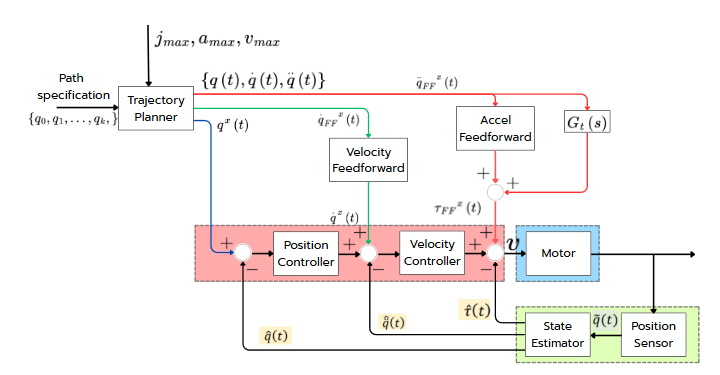
\includegraphics[width=\textwidth]{fig_cascade_pid_block_ch3}
    \caption{Block Diagram ของระบบควบคุม Cascade PID
             แสดง Position Outer Loop, Velocity Inner Loop,
             Feedforward 3 ช่องทาง และ Anti-windup Back-calculation}
    \label{fig:cascade_pid_block_ch3}
\end{figure}

% -----------------------------------------------------------------------
\subsubsection{การแปลง Requirements เป็น Desired Pole Locations}
% -----------------------------------------------------------------------

จาก P6 (Overshoot $\leq 1\%$) เลือก $\zeta = 0.9$
ซึ่งให้ Overshoot ตามสมการ

\begin{equation}
    \%OS = e^{-\pi\zeta/\sqrt{1-\zeta^2}} \times 100
         = e^{-6.486} \times 100
         = 0.152\% \leq 1\%
    \quad\checkmark
    \label{eq:os_check}
\end{equation}

จาก P5 (Settling Time $\leq 0.5$\,s) ใช้สูตร 2\% Criterion

\begin{equation}
    \omega_{n,pos} \geq \frac{4}{\zeta\,t_s}
                       = \frac{4}{0.9 \times 0.5}
                       = 8.889\,\text{rad/s}
    \label{eq:wn_req}
\end{equation}

Desired Poles ของ Position Loop

\begin{equation}
    s^*_{pos} = -\zeta\,\omega_{n,pos}
                \pm j\,\omega_{n,pos}\sqrt{1-\zeta^2}
              = -8.000 \pm j3.875
    \label{eq:s_des_pos}
\end{equation}

% -----------------------------------------------------------------------
\subsubsection{Velocity Inner Loop (PI)}
% -----------------------------------------------------------------------

\paragraph{การกำหนด Bandwidth Separation}

ระบบ Cascade PID นี้ใช้ Sampling Rate ที่แตกต่างกันสองระดับ
ได้แก่ Position Loop ที่ $f_{p} = 100$\,Hz ($T_p = 10$\,ms)
และ Velocity Loop ที่ $f_{v} = 1{,}000$\,Hz ($T_v = 1$\,ms)
อัตราส่วน Sampling Rate ระหว่างสองวงรอบจึงเป็น 10 เท่าพอดี

การกำหนด Bandwidth Separation ให้สอดคล้องกับอัตราส่วนนี้
มีเหตุผลทางปฏิบัติที่ชัดเจน ได้แก่
หาก $\omega_{n,vel}$ สูงกว่า $\omega_{n,pos}$ น้อยกว่า 10 เท่า
Velocity Loop จะมี Bandwidth ใกล้เคียงกับ
Nyquist Frequency ของ Position Loop ($f_{p}/2 = 50$\,Hz)
ซึ่งทำให้ Position Controller มองเห็น Velocity Loop
เป็น Unity Gain ได้ไม่สมบูรณ์
และเกิด Interaction ระหว่างสองวงรอบ
ดังนั้นจึงกำหนด

\begin{equation}
    \omega_{n,vel} = 10 \times \omega_{n,pos}
                  = 10 \times 8.889
                  = 88.889\,\text{rad/s}
    \label{eq:bw_sep}
\end{equation}

\textbf{หมายเหตุ:} การกำหนด Bandwidth Separation เป็น Heuristic
ไม่ใช่ทฤษฎีเคร่งครัด วรรณกรรมทั่วไปแนะนำค่าระหว่าง 5--10 เท่า
โครงงานนี้เลือก 10 เท่าเนื่องจากสอดคล้องกับอัตราส่วน
Sampling Rate ของ Hardware จริง
ความถูกต้องของการเลือกนี้ยืนยันได้จากผล Simulation
ที่แสดงว่า Velocity Loop ตอบสนองเร็วกว่า Position Loop
อย่างมีนัยสำคัญ

Desired Poles ของ Velocity Loop คือ
$s^*_{vel} = -\zeta\,\omega_{n,vel} \pm j\,\omega_{n,vel}\sqrt{1-\zeta^2}
           = -80.000 \pm j38.747$

\paragraph{การ Reduce Plant จาก 2nd-order เป็น 1st-order}

Full Velocity Plant จาก\cref{eq:Gvel_num} มีสองโพล ได้แก่
Electrical Pole ที่ $s = -R_a/L_a \approx -1004$\,rad/s
และ Mechanical Pole ที่ $s = -B/J \approx -0.265$\,rad/s
เนื่องจาก Desired Bandwidth ของ Velocity Loop คือ
$\omega_{n,vel} = 88.889$\,rad/s ซึ่งน้อยกว่า
$R_a/L_a$ ถึง 11 เท่า

\begin{equation}
    \frac{R_a}{L_a} = \frac{1.4534}{0.001448} = 1003.7\,\text{rad/s}
    \gg \omega_{n,vel} = 88.889\,\text{rad/s}
    \label{eq:elec_pole_check}
\end{equation}

Electrical Dynamics จึงดับลงเร็วมากและถูกมองเป็น
Algebraic Gain จากมุมมองของ Velocity Controller
สามารถตั้งสมมติฐาน $L_a \approx 0$ ได้
วงจรไฟฟ้าใน\cref{eq:electrical_ode} ลดรูปเป็น

\begin{equation}
    i_a \approx \frac{V_a - K_b N \omega}{R_a}
    \label{eq:ia_reduced}
\end{equation}

แทน\cref{eq:ia_reduced} ลงใน\cref{eq:mechanical_ode}
แล้วจัดรูปได้ Reduced 1st-order Plant

\begin{equation}
    \tilde{G}_v(s) = \frac{\omega(s)}{V_a(s)}
                   = \frac{K_{eq}}{J\,s + b_{eq}}
    \label{eq:Gv_red}
\end{equation}

\noindent โดยที่ $b_{eq}$ คือ Viscous Damping สมมูล
ซึ่งรวม Mechanical Damping $B$ และ Back-EMF Damping
$K_b K_t N^2 \eta / R_a$ เข้าด้วยกัน
และ $K_{eq}$ คือ DC Gain สมมูลของ Plant

\begin{equation}
    \begin{aligned}
        b_{eq} &= B + \frac{K_b K_t N^2 \eta}{R_a} \\
               &= 0.19279 + \frac{0.04165 \times 0.04065 \times 70^2 \times 0.836}{1.4534} \\
               &= 0.193 + 4.772 \\
               &= 4.9647 \, \mathrm{N \cdot m \cdot s/rad}
    \end{aligned}
    \label{eq:beq}
\end{equation}

\begin{equation}
    \begin{aligned}
        K_{eq} &= \frac{\eta \, K_t \, N}{R_a} \\
               &= \frac{0.836 \times 0.04065 \times 70}{1.4534} \\
               &= 1.6367 \, \mathrm{N \cdot m/V}
    \end{aligned}
    \label{eq:Keq}
\end{equation}

สังเกตว่า Back-EMF Damping ($4.772$) มีขนาดใหญ่กว่า
Mechanical Damping ($0.193$) ถึง 25 เท่า
แสดงว่า Damping หลักของระบบนี้มาจาก Back-EMF
ไม่ใช่จาก Bearing Friction

แทนค่าตัวเลขได้ Reduced Plant

\begin{equation}
    \tilde{G}_v(s) = \frac{1.6367}{0.7276\,s + 4.9647}
    \label{eq:Gv_red_num}
\end{equation}

% -----------------------------------------------------------------------
% รูปที่: Root Locus — Velocity Inner Loop
% ชื่อไฟล์แนะนำ: fig_rlocus_velocity.png
% เนื้อหา: Root Locus ของ PI × G_v_reduced(s)
%          Desired Poles s* = -80 ± j38.7 แสดงด้วย * สีแดง
%          เส้นประสีน้ำเงินแสดง Damping Ratio ζ = 0.9
% -----------------------------------------------------------------------
\begin{figure}[H]
    \centering
    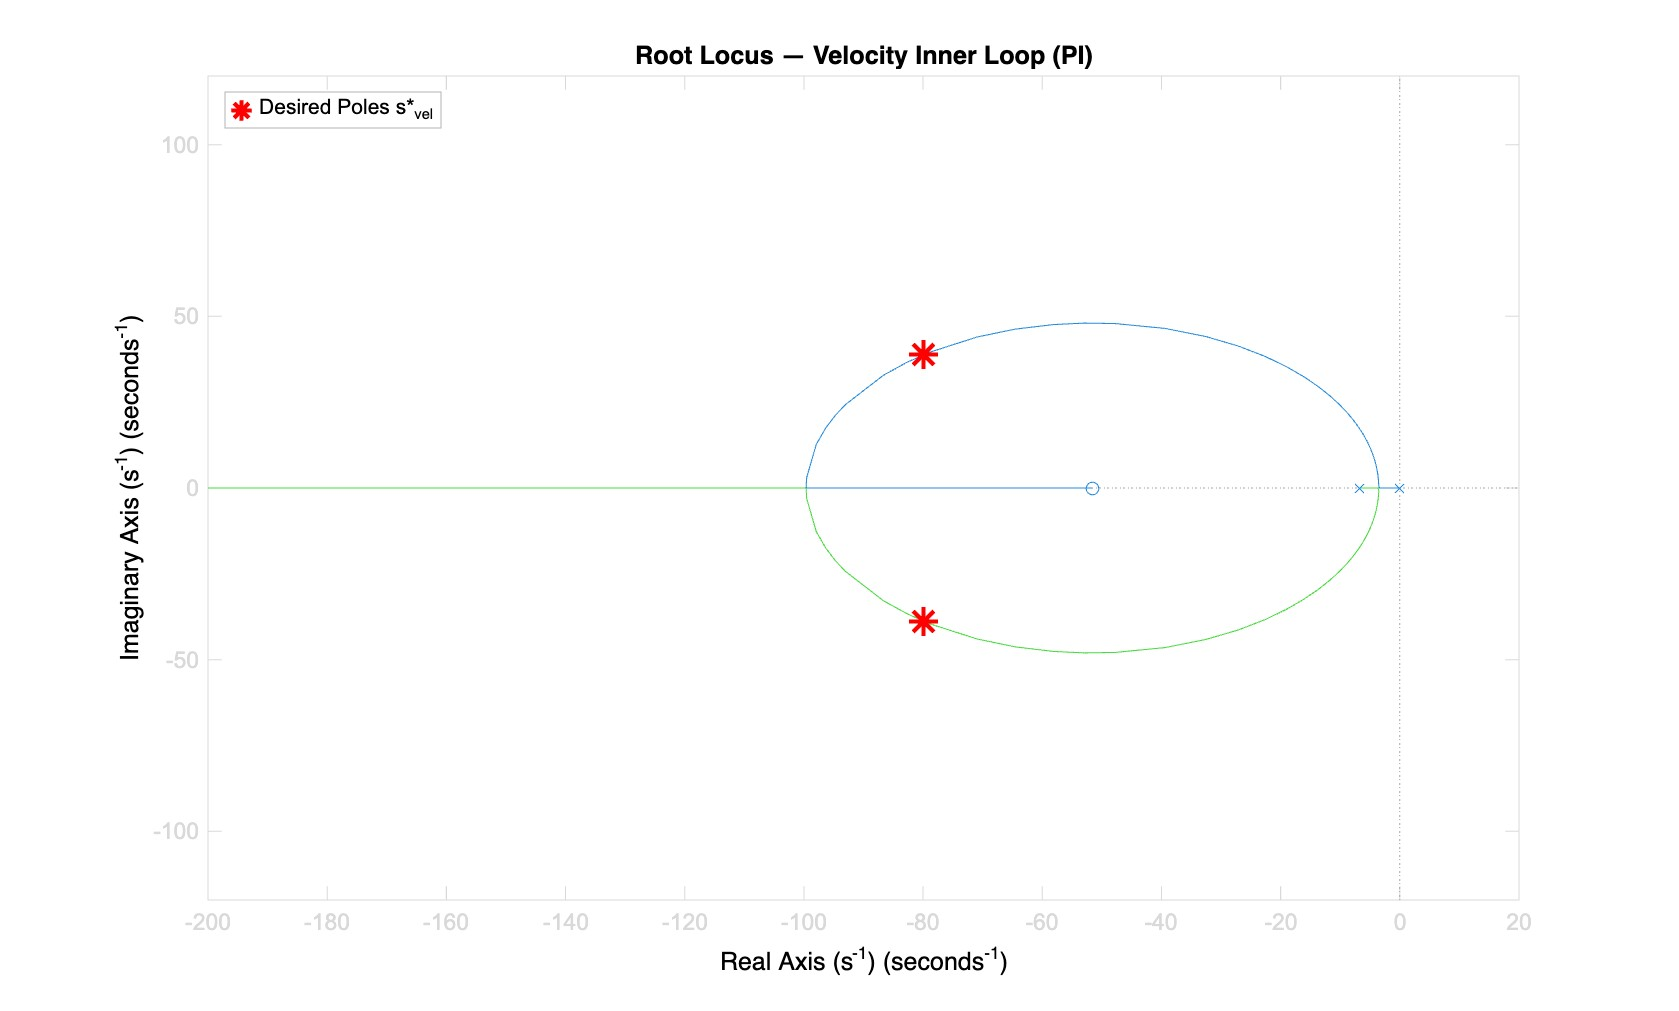
\includegraphics[width=1\textwidth]{fig_rlocus_velocity}
    \caption{Root Locus ของ Velocity Inner Loop (PI + Reduced Plant)
             แสดง Desired Poles $s^*_{vel} = -80.000 \pm j38.747$
             (เครื่องหมาย $\times$ สีแดง) บนเส้น Damping Ratio
             $\zeta = 0.9$ (เส้นประสีน้ำเงิน)}
    \label{fig:rlocus_velocity}
\end{figure}

\paragraph{การคำนวณ Velocity PI Gains}

ใช้ Pole Placement บน Reduced Plant
โดย Characteristic Equation ของ Closed-loop
Velocity Loop ที่ต้องการคือ

\begin{equation}
    s^2 + 2\zeta\,\omega_{n,vel}\,s + \omega_{n,vel}^2
    = s^2 + 160.000\,s + 7901.235
    \label{eq:vel_char}
\end{equation}

เทียบสัมประสิทธิ์กับ Closed-loop Characteristic Equation
ของ PI + 1st-order Plant ได้

\begin{align}
    K_{p,vel} &= \frac{2\zeta\,\omega_{n,vel}\,J - b_{eq}}{K_{eq}}
              = \frac{2 \times 0.9 \times 88.889 \times 0.72762 - 4.9647}{1.6367}
              = 68.940
    \label{eq:Kpv} \\[6pt]
    K_{i,vel} &= \frac{\omega_{n,vel}^2\,J}{K_{eq}}
              = \frac{(88.889)^2 \times 0.72762}{1.6367}
              = 3512.963
    \label{eq:Kiv}
\end{align}

% -----------------------------------------------------------------------
\subsubsection{Position Outer Loop (P)}
% -----------------------------------------------------------------------

เมื่อ Velocity Loop ปิดแล้วและ Bandwidth Separation
เป็น 10 เท่า Closed-loop Velocity Transfer Function
มีค่าใกล้เคียง Unity ในย่านที่ Position Loop ทำงาน
Plant สำหรับ Position Loop จึงประมาณได้เป็น Integrator

\begin{equation}
    G_{pos,plant}(s) \approx \frac{1}{s}
    \label{eq:pos_plant_approx}
\end{equation}

ใช้ P Controller เพียงอย่างเดียว
เนื่องจาก Integrator ใน Plant ทำให้ Steady-State Error
ต่อ Step Position Command เป็นศูนย์โดยธรรมชาติ
โดยไม่ต้องการ Integral Term เพิ่มเติม

\begin{equation}
    K_{p,pos} = \omega_{n,pos} = 8.889\,\text{s}^{-1}
    \quad\Rightarrow\quad
    t_s = \frac{4}{K_{p,pos}} = 0.450\,\text{s} \leq 0.5\,\text{s}
    \quad\checkmark
    \label{eq:Kpp}
\end{equation}

% -----------------------------------------------------------------------
% รูปที่: Root Locus — Position Outer Loop
% ชื่อไฟล์แนะนำ: fig_rlocus_position.png
% เนื้อหา: Root Locus ของ P × (1/s)
%          Desired Poles s* = -8 ± j3.875 แสดงด้วย * สีแดง
%          เส้นประสีน้ำเงินแสดง Damping Ratio ζ = 0.9
% -----------------------------------------------------------------------
\begin{figure}[H]
    \centering
    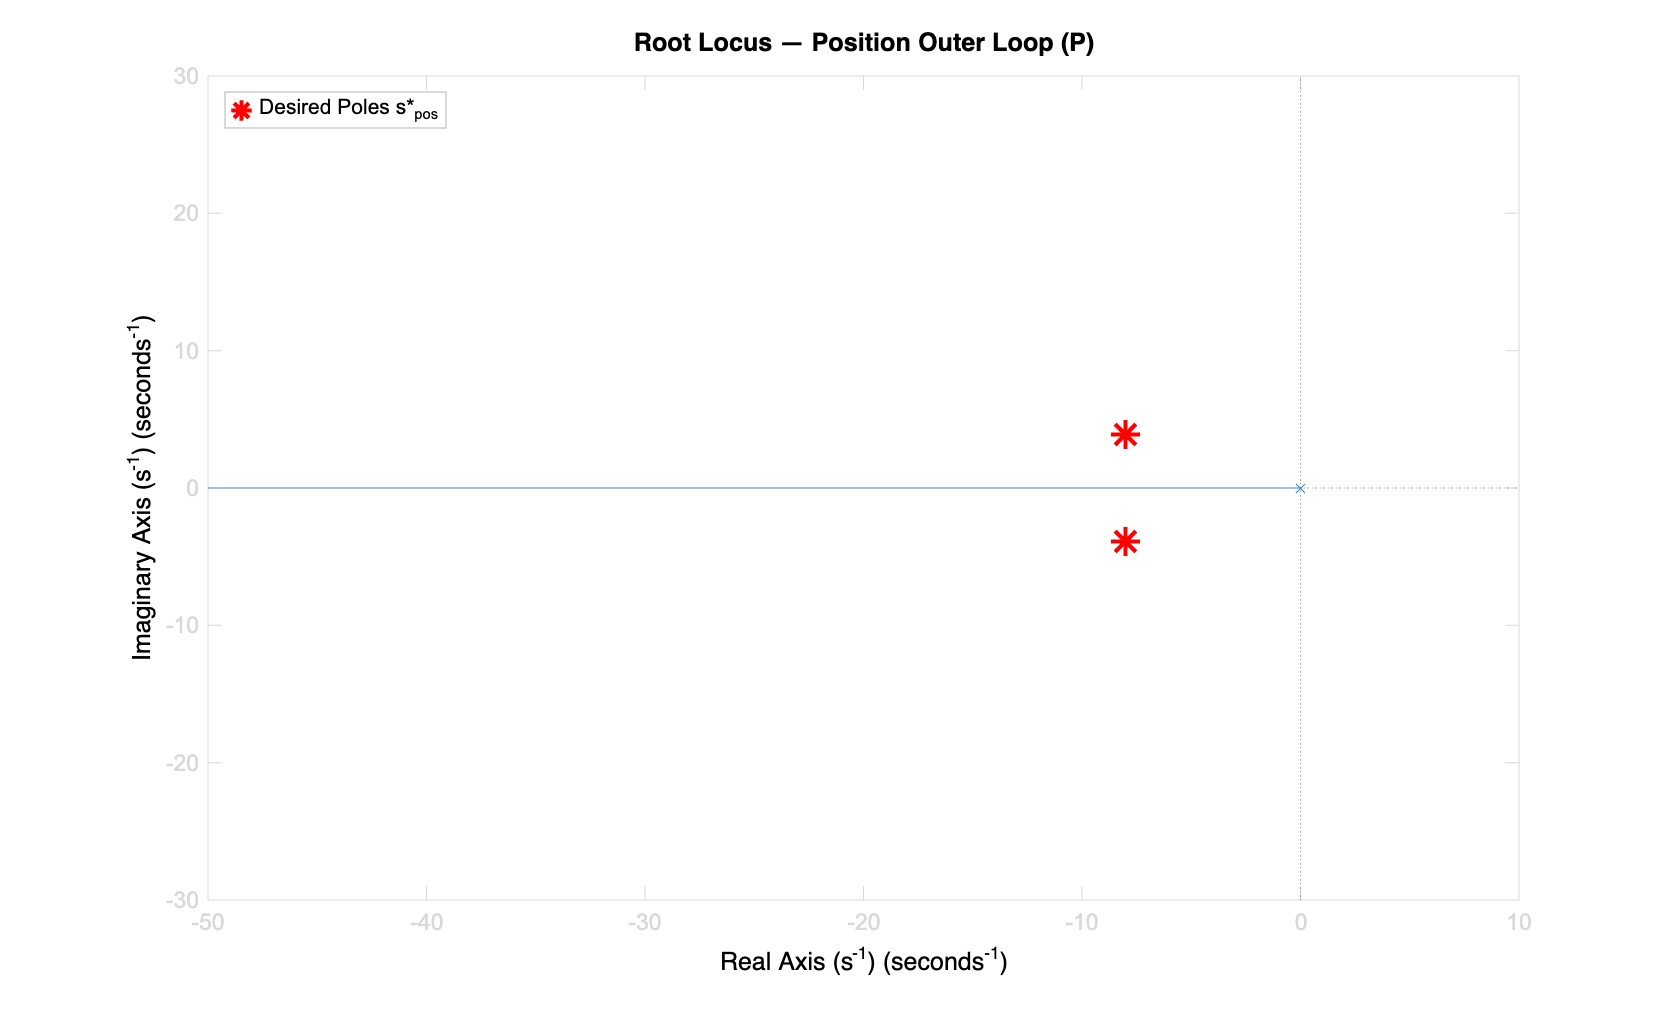
\includegraphics[width=1\textwidth]{fig_rlocus_position}
    \caption{Root Locus ของ Position Outer Loop (P + Integrator Plant)
             แสดง Desired Poles $s^*_{pos} = -8.000 \pm j3.875$
             (เครื่องหมาย $\times$ สีแดง) บนเส้น Damping Ratio
             $\zeta = 0.9$ (เส้นประสีน้ำเงิน)}
    \label{fig:rlocus_position}
\end{figure}

% -----------------------------------------------------------------------
\subsubsection{Anti-windup และ Feedforward}
% -----------------------------------------------------------------------

\paragraph{Anti-windup Back-calculation}

Velocity Loop มี $K_{i,vel}$ ขนาดใหญ่
ทำให้เมื่อเกิด Large Setpoint Change
Integrator State สะสมค่าสูงก่อนที่แรงดัน Output
จะถึง Saturation Limit $\pm 24$\,V (Integral Windup)
Anti-windup แบบ Back-calculation แก้ปัญหานี้
โดยป้อนกลับส่วนต่างระหว่าง Unsaturated
และ Saturated Output มาลด Integrator State
ตามที่อธิบายใน\cref{eq:anti_windup}

\begin{equation}
    K_{t,aw} = \frac{K_{i,vel}}{K_{p,vel}}
             = \frac{3512.963}{68.940}
             = 50.958\,\text{s}^{-1}
    \label{eq:Ktaw}
\end{equation}

\paragraph{Feedforward Gains}

Feedforward ช่วยลด Tracking Error ระหว่างการเคลื่อนที่
โดยไม่ต้องรอ Error สะสมก่อน
ระบบนี้มี Feedforward 3 ช่องทาง

\textbf{Velocity Feedforward ($K_{vff}$):}
ในสภาวะ Steady-State ที่ความเร็วคงที่
($\dot{\omega} = 0$, $\tau_d = 0$)
แทนค่าลงใน\cref{eq:mechanical_ode} และ\cref{eq:electrical_ode}
ได้แรงดันที่จำเป็น

\begin{equation}
    K_{vff} = \frac{R_a\,B}{\eta\,N\,K_t} + K_b\,N
            = \frac{1.4534 \times 0.19279}{0.836 \times 70 \times 0.04065}
              + 0.04165 \times 70
            = 0.117 + 2.916
            = 3.033\,\text{V/(rad/s)}
    \label{eq:kvff}
\end{equation}

\textbf{Acceleration Feedforward ($K_{aff}$):}
ในสภาวะที่มีความเร่ง $\dot{\omega} \neq 0$
แรงบิดส่วนที่ใช้เร่งมวล $J\dot{\omega}$
ต้องการแรงดันเพิ่มเติม

\begin{equation}
    K_{aff} = \frac{R_a\,J}{\eta\,N\,K_t}
            = \frac{1.4534 \times 0.72762}{0.836 \times 70 \times 0.04065}
            = \frac{1.0577}{2.376}
            = 0.445\,\text{V/(rad/s}^2\text{)}
    \label{eq:kaff}
\end{equation}

\textbf{Torque Disturbance Feedforward ($K_{tff}$):}
หาก Kalman Filter ประมาณค่า Disturbance Torque $\hat{\tau}_d$
ได้แล้ว สามารถชดเชยล่วงหน้าได้โดย

\begin{equation}
    \begin{aligned}
        K_{tff} &= \frac{R_a}{\eta \, N \, K_t} \\
                &= \frac{1.4534}{0.836 \times 70 \times 0.04065} \\
                &= \frac{1.4534}{2.376} \\
                &= 0.612 \, \mathrm{V/(N \cdot m)}
    \end{aligned}
    \label{eq:ktff}
\end{equation}

\noindent โดย $K_{tff}$ เปิดใช้งานเมื่อ Kalman Filter
Converge แล้วเท่านั้น ตามที่อธิบายใน\cref{subsec:kalman_filter}

\begin{table}[H]
  \centering
  \caption{สรุปค่า PID Gain และ Feedforward ของระบบควบคุม}
  \label{tab:pid_gains}
  \begin{tabular}{llccc}
    \toprule
    Loop & Gain & สัญลักษณ์ & ค่า & หน่วย \\
    \midrule
    \multirow{2}{*}{Velocity Inner (PI)}
      & Proportional & $K_{p,vel}$ & 68.940   & V/(rad/s) \\
      & Integral     & $K_{i,vel}$ & 3512.963 & V/rad \\
    \midrule
    Anti-windup
      & Back-calc    & $K_{t,aw}$  & 50.958   & s$^{-1}$ \\
    \midrule
    Position Outer (P)
      & Proportional & $K_{p,pos}$ & 8.889    & (rad/s)/rad \\
    \midrule
    \multirow{3}{*}{Feedforward}
      & Velocity FF      & $K_{vff}$ & 3.033 & V/(rad/s) \\
      & Acceleration FF  & $K_{aff}$ & 0.445 & V/(rad/s$^2$) \\
      & Disturbance FF   & $K_{tff}$ & 0.612 & V/(N$\cdot$m) \\
    \bottomrule
    \multicolumn{5}{l}{\small หมายเหตุ: $K_{vff}$, $K_{aff}$, $K_{tff}$
      ปิดระหว่าง Commissioning} \\
    \multicolumn{5}{l}{\small จนกว่า SysID uncertainty $< 10\%$
      และ Kalman Filter Converge} \\
  \end{tabular}
\end{table}

% -----------------------------------------------------------------------
\subsubsection{Hardware Commissioning และค่า Gain จริง}
\label{subsubsec:hw_commissioning}
% -----------------------------------------------------------------------

ค่า Gain ที่ได้จาก Pole Placement ใน\cref{eq:Kpv,eq:Kiv,eq:Kpp}
คำนวณภายใต้สมมติฐานว่าแบบจำลอง Plant มีความแม่นยำสมบูรณ์
และ Output ของ Controller คือแรงดัน $V_a$ ในหน่วย Volt
อย่างไรก็ตาม Firmware จริงบน STM32G474RE
ส่งคำสั่งในรูป PWM Count ($0$ ถึง $\pm$50)
ผ่านฟังก์ชัน \texttt{Motor\_SetPWM()} โดยมี Scale Factor

\begin{equation}
    \text{Scale} = \frac{V_{supply}}{PWM_{max}}
                 = \frac{24}{50}
                 = 0.48\,\text{V/PWM}
    \label{eq:pwm_scale}
\end{equation}

ดังนั้น Theoretical Gains ที่แปลงหน่วยเป็น PWM Unit แล้วคือ

\begin{equation}
    K_{p,vel}^{theory,hw}
        = \frac{K_{p,vel}^{theory}}{\text{Scale}}
        = \frac{68.940}{0.48}
        \approx 143.6\,\text{PWM/(rad/s)}
    \label{eq:Kpv_scaled}
\end{equation}

ซึ่งยังคงสูงกว่าค่าที่ใช้งานได้จริงอย่างมีนัยสำคัญ
เนื่องจากปัจจัยหลักสามประการ ได้แก่

\begin{itemize}
    \item \textbf{Model Uncertainty:}
          พารามิเตอร์ $J = 0.728\,\text{kg·m}^2$ และ $B = 0.193\,\text{N·m·s/rad}$
          ประมาณจาก Chirp Excitation ที่ความถี่ต่ำ (0.1--2\,Hz)
          ซึ่งอาจไม่สะท้อน Dynamic ของระบบที่ Bandwidth สูงกว่าได้อย่างแม่นยำ

    \item \textbf{Nonlinearity:}
          แบบจำลอง LTI ละทิ้ง Static Friction ของ Bearing และ Belt Drive
          ซึ่งมีผลต่อ Gain ที่เหมาะสมในสภาวะ Low-Velocity

    \item \textbf{PWM Saturation:}
          Gain สูงทำให้ Controller Output Saturate ที่ $\pm$50 PWM
          ในช่วง Transient เกือบตลอดเวลา
          ทำให้ระบบไม่ทำงานในย่าน Linear ตามที่ Pole Placement สมมติ
\end{itemize}

ด้วยเหตุนี้ Theoretical Gains จึงใช้เป็น \textbf{Order-of-Magnitude Reference}
และ \textbf{Starting Point} สำหรับ Hardware Commissioning เท่านั้น
ไม่ใช่ค่าที่นำไปใช้งานโดยตรง

\paragraph{ขั้นตอน Hardware Commissioning}

ดำเนินการ Tune Gains บน Hardware จริงตามลำดับดังนี้

\begin{enumerate}
    \item \textbf{Velocity Loop ก่อน:}
          ปิด Position Loop ชั่วคราว
          เพิ่ม $K_{p,vel}$ ทีละน้อยจนระบบเริ่ม Oscillate
          บันทึก $K_{p,crit}$ แล้วลดลงเหลือประมาณ $0.5 \times K_{p,crit}$
          จากนั้นเพิ่ม $K_{i,vel}$ ช้าๆ จนกำจัด Steady-State Error ได้

    \item \textbf{Position Loop ถัดไป:}
          เปิด Position Loop แล้วเพิ่ม $K_{p,pos}$ ทีละน้อย
          จนได้ Response ที่เร็วเพียงพอโดยไม่มี Overshoot
          จากนั้นปรับ $K_{d,pos}$ เพื่อ Damp การสั่น
          และ $K_{i,pos}$ เพื่อกำจัด Steady-State Error จาก Friction

    \item \textbf{ตรวจสอบ Requirements:}
          วัด Settling Time และ Overshoot จากการทดสอบ Step Response
          บน Hardware จริง เทียบกับ P5 ($t_s \leq 0.5$\,s)
          และ P6 (\%OS $\leq 1\%$)
\end{enumerate}

\subsection{ค่า Gain ที่ใช้งานจริง (Hardware-Tuned)}

\begin{table}[H]
  \centering
  \caption{เปรียบเทียบค่า PID Gain จาก Theoretical Design
           และ Hardware Commissioning}
  \label{tab:pid_gains_comparison}
  \begin{tabular}{llcccc}
    \toprule
    Loop & สัญลักษณ์ & Theoretical & Hardware & หน่วย (Theory) & หน่วย (HW) \\
    \midrule
    \multirow{2}{*}{Velocity (PI)}
      & $K_{p,vel}$ & 68.940   & [HW\_KPV] & V/(rad/s)      & PWM/(rad/s) \\
      & $K_{i,vel}$ & 3512.963 & [HW\_KIV] & V/rad          & PWM/rad     \\
    \midrule
    \multirow{3}{*}{Position (PID)}
      & $K_{p,pos}$ & 8.889  & [HW\_KPP] & (rad/s)/rad & (rad/s)/rad \\
      & $K_{i,pos}$ & --     & [HW\_KIP] & --          & (rad/s)/(rad·s) \\
      & $K_{d,pos}$ & --     & [HW\_KDP] & --          & (rad/s)·s/rad \\
    \midrule
    Anti-windup
      & $K_{t,aw}$  & 50.958 & [HW\_KAW] & s$^{-1}$ & s$^{-1}$ \\
    \midrule
    \multirow{3}{*}{Feedforward}
      & $K_{vff}$ & 3.033 & [HW\_KVFF] & V/(rad/s)     & PWM/(rad/s) \\
      & $K_{aff}$ & 0.445 & [HW\_KAFF] & V/(rad/s$^2$) & PWM/(rad/s$^2$) \\
      & $K_{tff}$ & 0.612 & [HW\_KTFF] & V/(N·m)       & PWM/(N·m) \\
    \bottomrule
    \multicolumn{6}{l}{\small [HW\_*] = ค่าที่ได้จาก Hardware Commissioning
      — อัปเดตหลัง Tuning เสร็จสิ้น} \\
  \end{tabular}
\end{table}

% -----------------------------------------------------------------------
% รูปที่: Step Response จาก Hardware Commissioning
% ชื่อไฟล์แนะนำ: fig_step_response_hw.png
% เนื้อหา: กราฟ Position (deg) vs Time (s) แสดง Step Response จริง
%          บน Hardware พร้อม annotation Settling Time และ Overshoot
%          เปรียบเทียบ Reference (เส้นประ) กับ Actual (เส้นทึบ)
% -----------------------------------------------------------------------
% \begin{figure}[H]
%     \centering
%     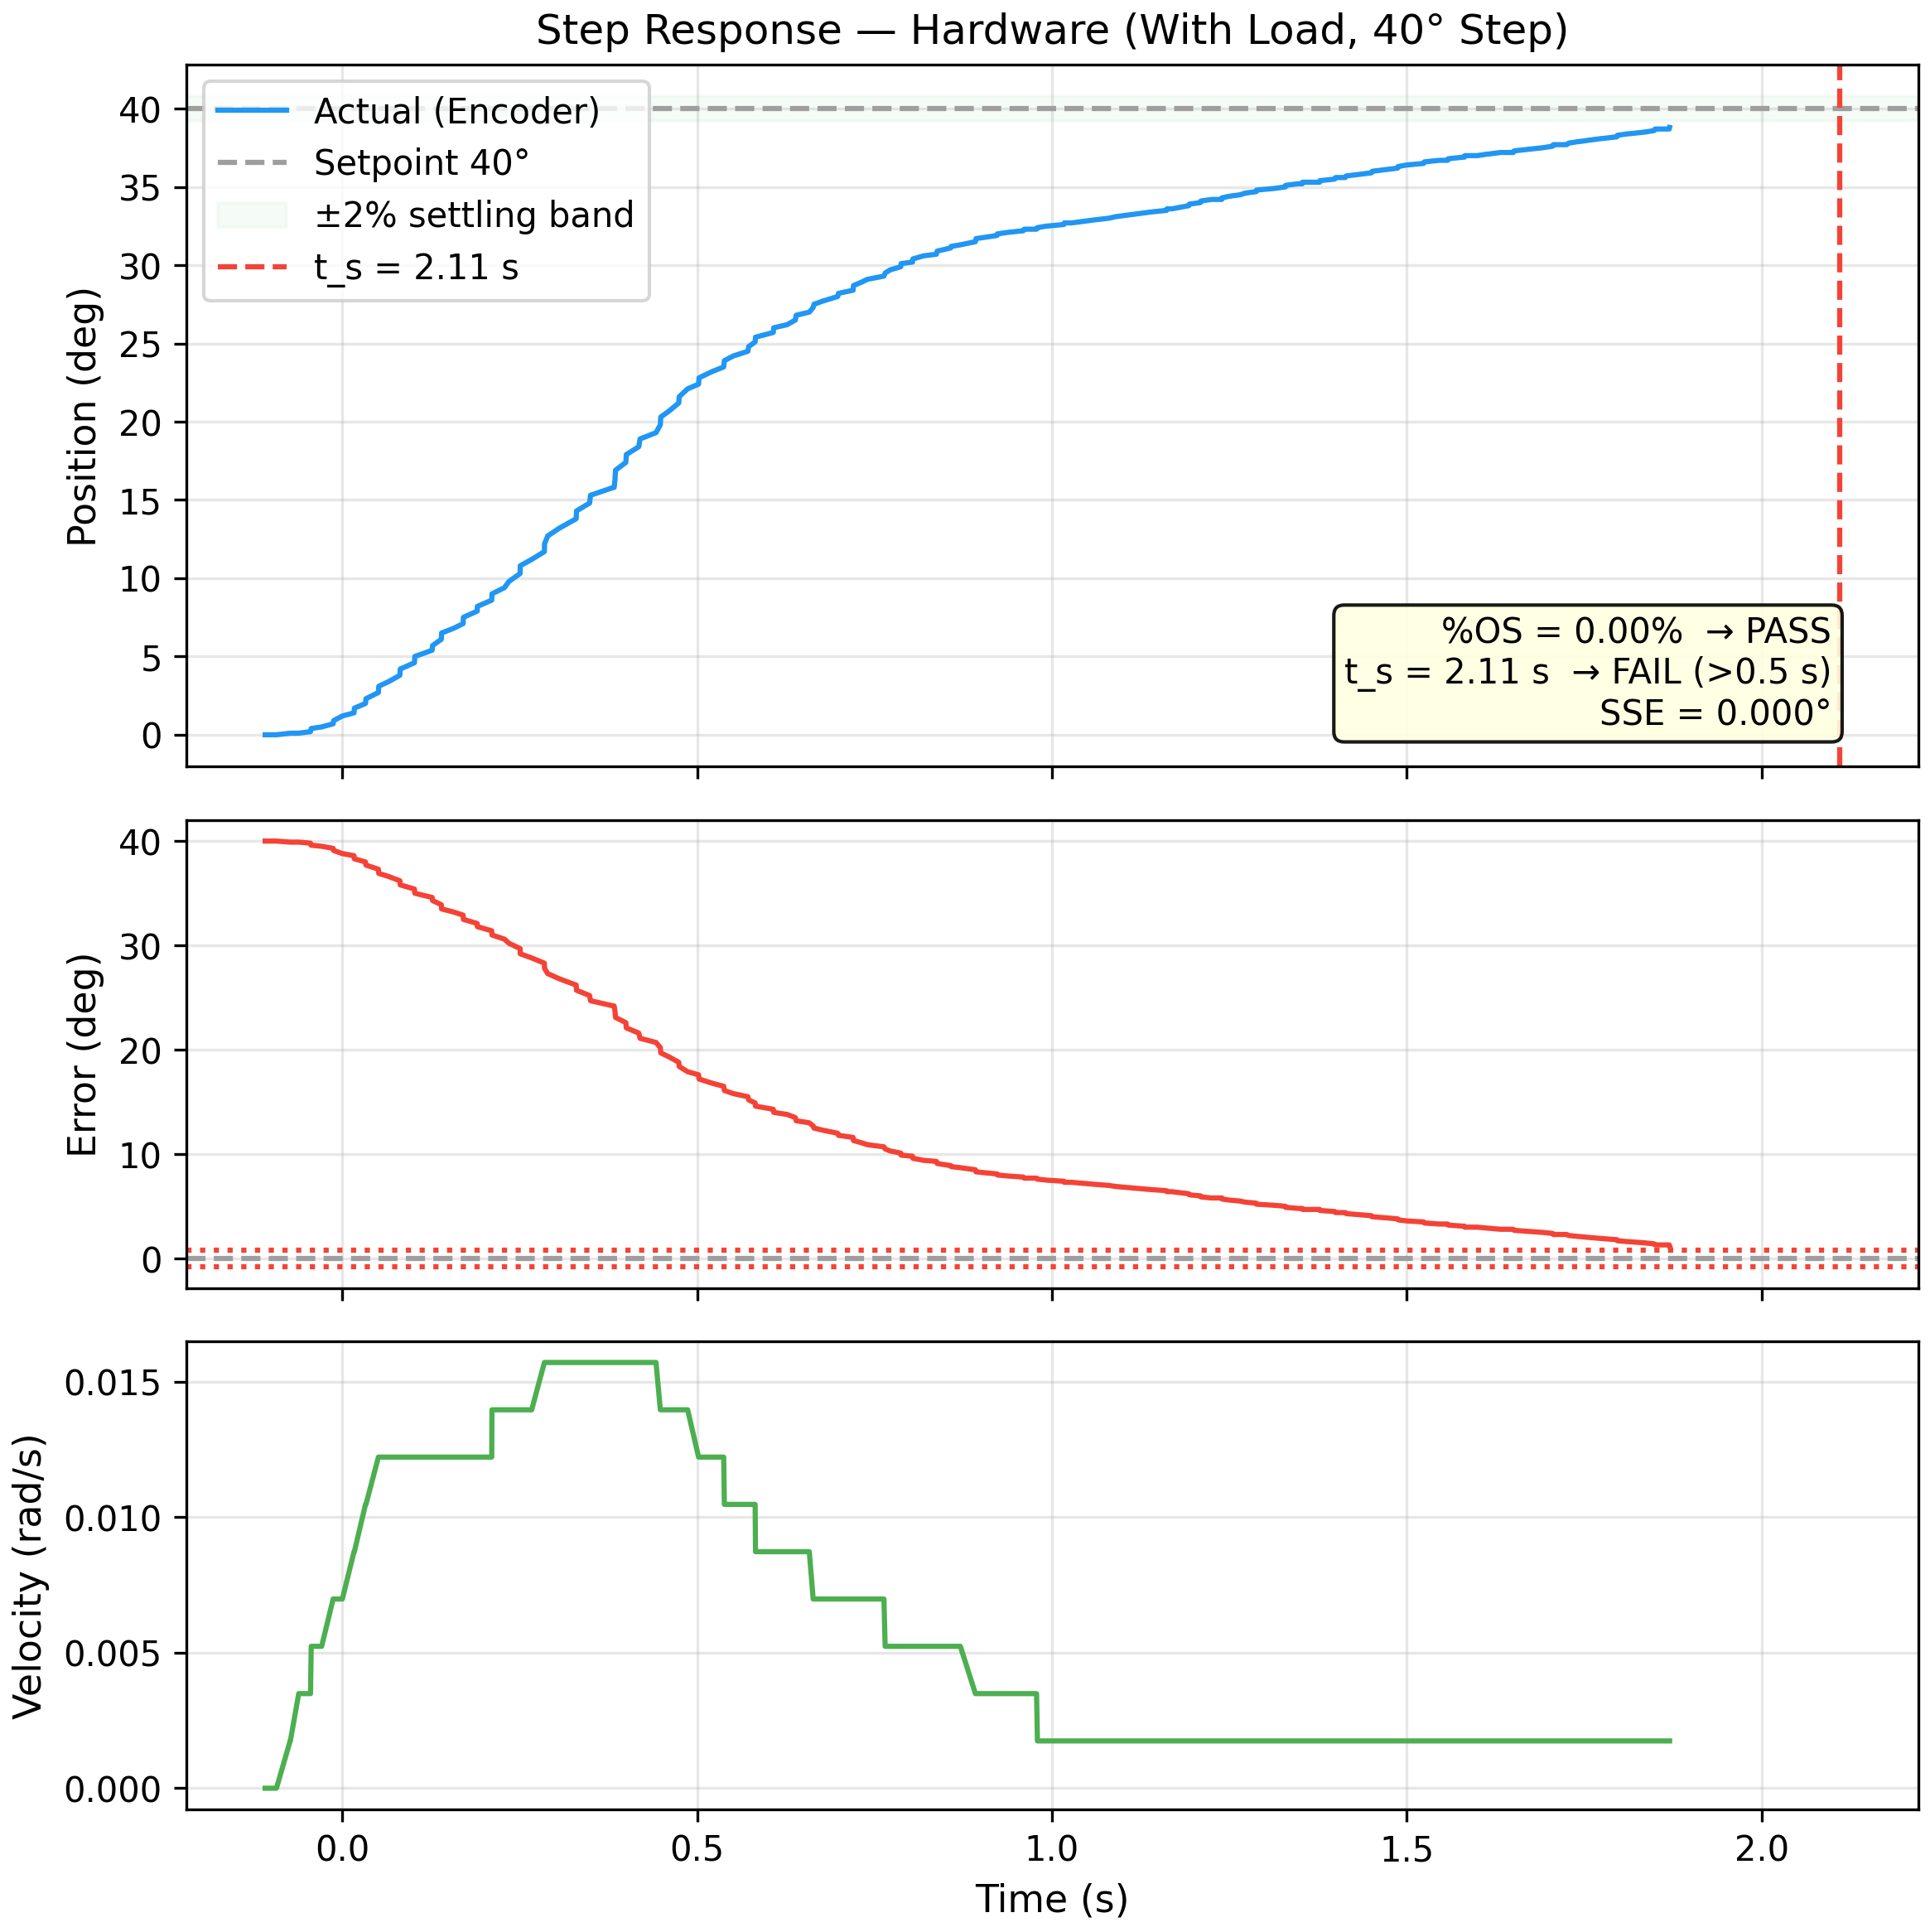
\includegraphics[width=0.85\textwidth]{fig_step_response_hw}
%     \caption{Step Response ของระบบ Cascade PID บน Hardware จริง
%              แสดง Settling Time และ Overshoot
%              เทียบกับข้อกำหนด P5 ($t_s \leq 0.5$\,s)
%              และ P6 (\%OS $\leq 1\%$)}
%     \label{fig:step_response_hw}
% \end{figure}

\begin{table}[H]
  \centering
  \caption{ผลการทดสอบ Step Response บน Hardware
           เทียบกับ Requirements}
  \label{tab:hw_step_results}
  \begin{tabular}{lcccc}
    \toprule
    Metric & ผล Hardware & Requirement & หน่วย & สถานะ \\
    \midrule
    Settling Time  & [HW\_TS]  & $\leq 0.5$ & s   & [STATUS\_P5] \\
    Overshoot      & [HW\_OS]  & $\leq 1$   & \%  & [STATUS\_P6] \\
    Steady-State Error & [HW\_SSE] & --      & deg & -- \\
    \bottomrule
    \multicolumn{5}{l}{\small [HW\_*] = อัปเดตหลังเก็บข้อมูลจาก Hardware} \\
  \end{tabular}
\end{table}

% \subsubsection{ผลการ Simulation}

% \begin{table}[H]
%   \centering
%   \caption{ผลการ Simulation Cascade PID เปรียบเทียบกับ Requirements}
%   \label{tab:sim_results}
%   \begin{tabular}{lcccc}
%     \toprule
%     Metric & Unshaped & ZV-Shaped & Requirement & สถานะ \\
%     \midrule
%     Settling Time (Arm)  & 0.450\,s & 0.450\,s & $\leq 0.5$\,s & \textbf{PASS} \\
%     Overshoot            & 0.00\%   & 0.00\%   & $\leq 1\%$    & \textbf{PASS} \\
%     Steady-state Error   & $0.004°$ & $0.004°$ & --            & -- \\
%     Rod Peak Deflection  & $21.7°$  & $9.9°$   & $\leq 0.57°$ (at rest) & -- \\
%     Rod Settling Time    & 6.44\,s  & $\approx 0$\,s & -- & -- \\
%     \bottomrule
%   \end{tabular}
% \end{table}

% -----------------------------------------------------------------------
\subsubsection{การ Discretize สู่ Z-Domain (Tustin Transform)}
\label{subsubsec:discretization}
% -----------------------------------------------------------------------

การ Implement ตัวควบคุม Cascade PID บน STM32G474RE
จำเป็นต้องแปลง Continuous-time Controller
ให้เป็น Discrete-time ก่อน
โดยใช้วิธี Tustin (Bilinear Transform)

\begin{equation}
    s \;\longleftarrow\; \frac{2}{T}\cdot\frac{z-1}{z+1}
    \label{eq:tustin_sub}
\end{equation}

เหตุผลที่เลือก Tustin แทน Forward Euler ได้แก่
Tustin Map โพลทุกตัวในครึ่งซ้ายของระนาบ $s$
ให้อยู่ภายใน Unit Circle ของระนาบ $z$ อย่างสมบูรณ์
ในขณะที่ Forward Euler อาจทำให้ Discrete System
ไม่เสถียรแม้ Continuous System จะเสถียร
โดยเฉพาะเมื่อ $K_i/f_s$ มีขนาดใหญ่
ตามที่อธิบายใน\cref{subsec:cascade_pid}

% -----------------------------------------------------------------------
\paragraph{Velocity Inner Loop — PI (Tustin)}
% -----------------------------------------------------------------------

Continuous-time PI Controller ของ Velocity Loop คือ

\begin{equation}
    C_v(s) = K_{p,vel} + \frac{K_{i,vel}}{s}
    \label{eq:Cv_ct}
\end{equation}

แทน\cref{eq:tustin_sub} ลงใน\cref{eq:Cv_ct}
ที่ Sample Time $T_v = 1$\,ms ได้

\begin{equation}
    C_v(z) = K_{p,vel}
           + K_{i,vel}\cdot\frac{T_v}{2}\cdot\frac{z+1}{z-1}
    \label{eq:Cv_z}
\end{equation}

จัดรูปให้ได้ Difference Equation
โดยกำหนด $u_v[k]$ เป็น PWM Output
และ $e_v[k] = \omega_{sp}[k] - \omega_{act}[k]$
เป็น Velocity Error

\begin{equation}
    u_v[k] = u_v[k-1]
           + \underbrace{\left(K_{p,vel} + \frac{K_{i,vel}\,T_v}{2}\right)}_{c_1}
             e_v[k]
           + \underbrace{\left(-K_{p,vel} + \frac{K_{i,vel}\,T_v}{2}\right)}_{c_2}
             e_v[k-1]
    \label{eq:vel_diff_eq}
\end{equation}

\noindent โดยที่

\begin{align}
    c_1 &= K_{p,vel} + \frac{K_{i,vel}\,T_v}{2}
         = 68.940 + \frac{3512.963 \times 0.001}{2}
         = 68.940 + 1.756
         = 70.696
    \label{eq:c1_vel} \\[4pt]
    c_2 &= -K_{p,vel} + \frac{K_{i,vel}\,T_v}{2}
         = -68.940 + 1.756
         = -67.184
    \label{eq:c2_vel}
\end{align}

Difference Equation นี้ implement ได้โดยตรงใน Firmware
โดยเก็บเพียง $u_v[k-1]$ และ $e_v[k-1]$
เป็น Static Variable ซึ่งมี Memory Footprint
เพียง 2 ตัวแปร Float (8 bytes) ต่อ Loop

% -----------------------------------------------------------------------
\paragraph{Position Outer Loop — PID (Tustin, Derivative on Measurement)}
% -----------------------------------------------------------------------

Continuous-time PID Controller ของ Position Loop คือ

\begin{equation}
    C_p(s) = K_{p,pos} + \frac{K_{i,pos}}{s} + K_{d,pos}\,s
    \label{eq:Cp_ct}
\end{equation}

แทน Tustin Transform ที่ $T_p = 10$\,ms
และใช้ Derivative on Measurement
(แทน Derivative on Error เพื่อป้องกัน Derivative Kick
เมื่อ Setpoint เปลี่ยนแบบ Step)

\begin{equation}
    \text{D-term} = -K_{d,pos}\,\frac{d\theta_{act}}{dt}
    \label{eq:d_on_meas}
\end{equation}

Difference Equation ของ Position PID คือ

\begin{align}
    u_p[k] &= K_{p,pos}\,e_p[k] \notag \\
            &+ \frac{K_{i,pos}\,T_p}{2}
               \bigl(e_p[k] + e_p[k-1]\bigr)
               + I_p[k-1] \notag \\
            &- K_{d,pos}\,\frac{\theta_{act}[k] - \theta_{act}[k-1]}{T_p}
    \label{eq:pos_diff_eq}
\end{align}

\noindent โดยที่ $I_p[k]$ คือ Integral State ที่ Update ตาม

\begin{equation}
    I_p[k] = I_p[k-1]
           + \frac{K_{i,pos}\,T_p}{2}
             \bigl(e_p[k] + e_p[k-1]\bigr)
    \label{eq:pos_integral_update}
\end{equation}

และ $u_p[k]$ คือ Velocity Setpoint
ที่ส่งเข้า Velocity Inner Loop
ซึ่ง Clamp ไว้ที่ $\pm v_{max} = \pm 7.304$\,rad/s

% -----------------------------------------------------------------------
\paragraph{Anti-windup ใน Discrete-time}
% -----------------------------------------------------------------------

ทั้งสอง Loop ใช้ Conditional Integration
เพื่อป้องกัน Integral Windup โดย

\begin{itemize}
    \item \textbf{Velocity Loop:}
          หยุด Integrate เมื่อ Feedforward Output
          ใกล้ Saturation Limit
          ($|u_{ff}| \geq PWM_{max} - 1$)
          เนื่องจากสภาวะดังกล่าว PID Output
          จะถูก Clamp อยู่ดีและ Integral State
          ที่สะสมต่อไปจะไม่มีผลต่อ Output จริง

    \item \textbf{Position Loop:}
          หยุด Integrate เมื่อ Position Error
          อยู่ภายใน Deadband
          ($|e_p| < \delta_{dead}$)
          ป้องกัน Windup ขณะจอดนิ่ง
\end{itemize}

% -----------------------------------------------------------------------
\begin{table}[H]
  \centering
  \caption{สรุปค่าสัมประสิทธิ์ Discrete-time Controller
           (Theoretical Gains, หน่วย V)}
  \label{tab:discrete_coeffs}
  \begin{tabular}{llccc}
    \toprule
    Loop & พารามิเตอร์ & สัญลักษณ์ & ค่า & หน่วย \\
    \midrule
    \multirow{4}{*}{Velocity PI}
      & Sample Time       & $T_v$  & 0.001   & s \\
      & Forward Coeff     & $c_1$  & 70.696  & V/(rad/s) \\
      & Backward Coeff    & $c_2$  & $-67.184$ & V/(rad/s) \\
      & Integral Clamp    & $I_{max,v}$ & \texttt{PID\_SPEED\_IMAX} & V \\
    \midrule
    \multirow{4}{*}{Position PID}
      & Sample Time       & $T_p$  & 0.010  & s \\
      & Proportional      & $K_{p,pos}$ & 8.889 & (rad/s)/rad \\
      & Integral Step     & $K_{i,pos}T_p/2$ & [HW\_KIP\_STEP] & (rad/s)/rad \\
      & Derivative        & $K_{d,pos}/T_p$ & [HW\_KDP\_RATE] & (rad/s)·s/rad \\
    \bottomrule
    \multicolumn{5}{l}{\small หมายเหตุ: ค่า [HW\_*] อัปเดตหลัง Hardware Commissioning} \\
  \end{tabular}
\end{table}

\begin{figure}[H]
    \centering
    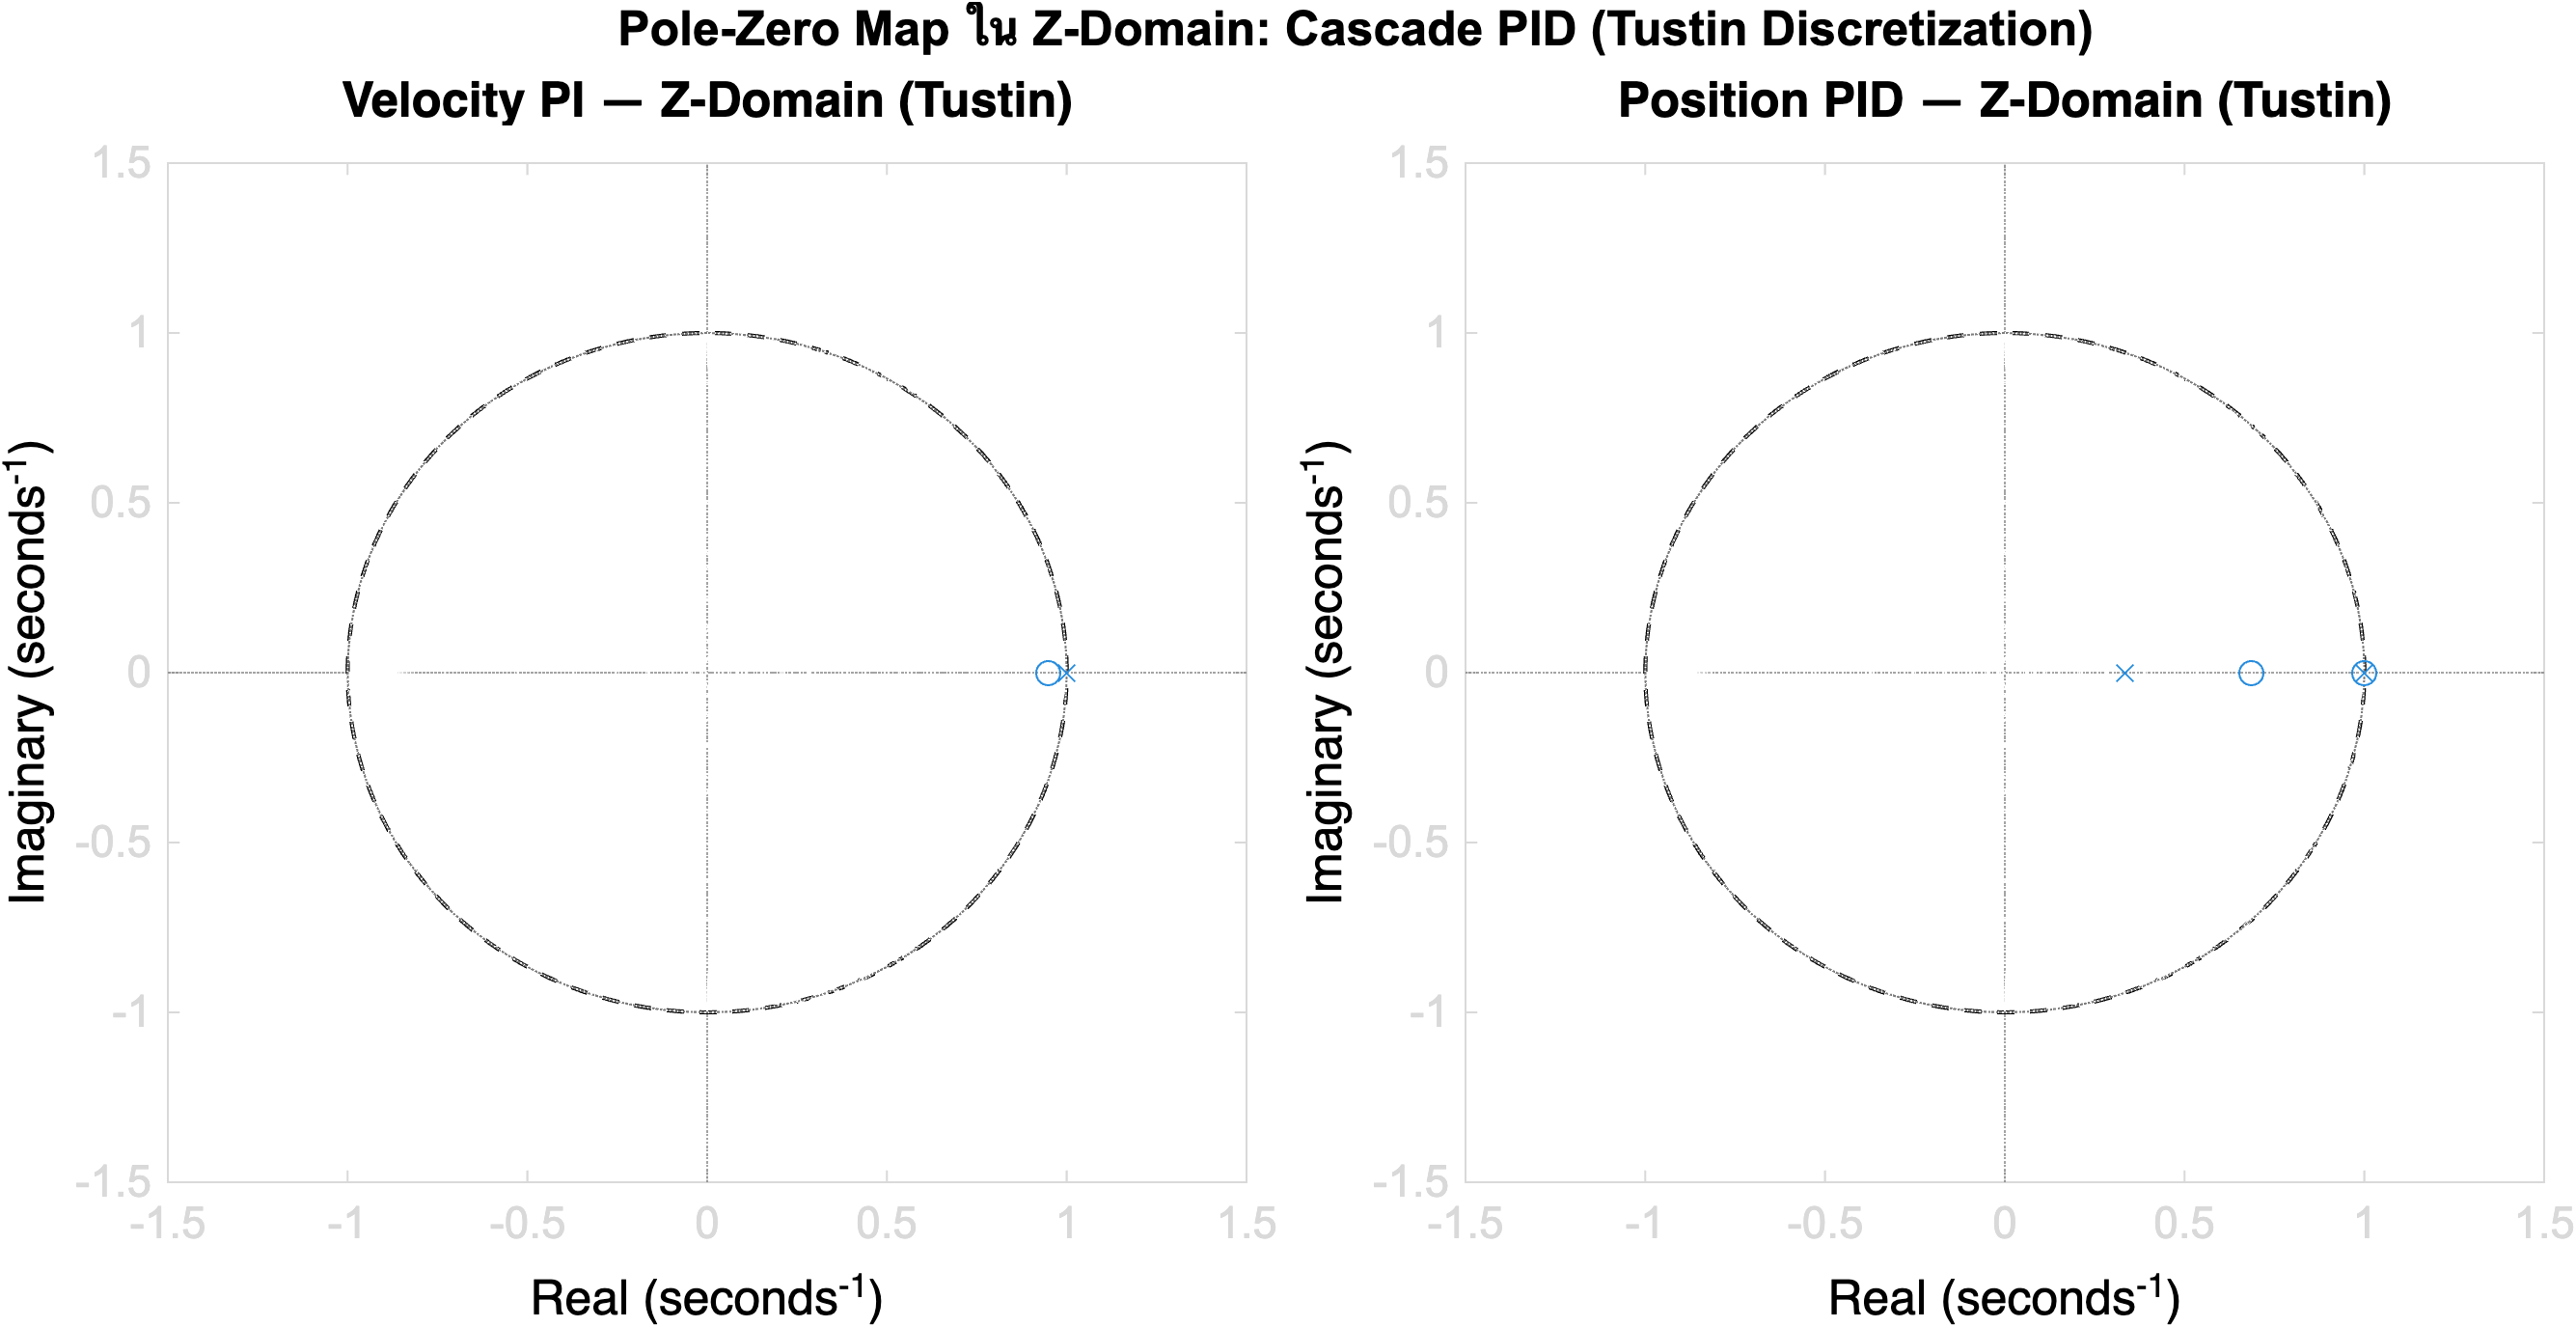
\includegraphics[width=0.90\textwidth]{fig_zpole_cascade}
    \caption{Pole-Zero Map ใน Z-Domain ของ Velocity PI (ซ้าย)
             และ Position PID (ขวา) หลัง Tustin Discretization
             Poles และ Zeros ทั้งหมดอยู่ภายใน Unit Circle
             ยืนยันความเสถียรของ Discrete-time Controller}
    \label{fig:zpole_cascade}
\end{figure}

\begin{figure}[H]
    \centering
    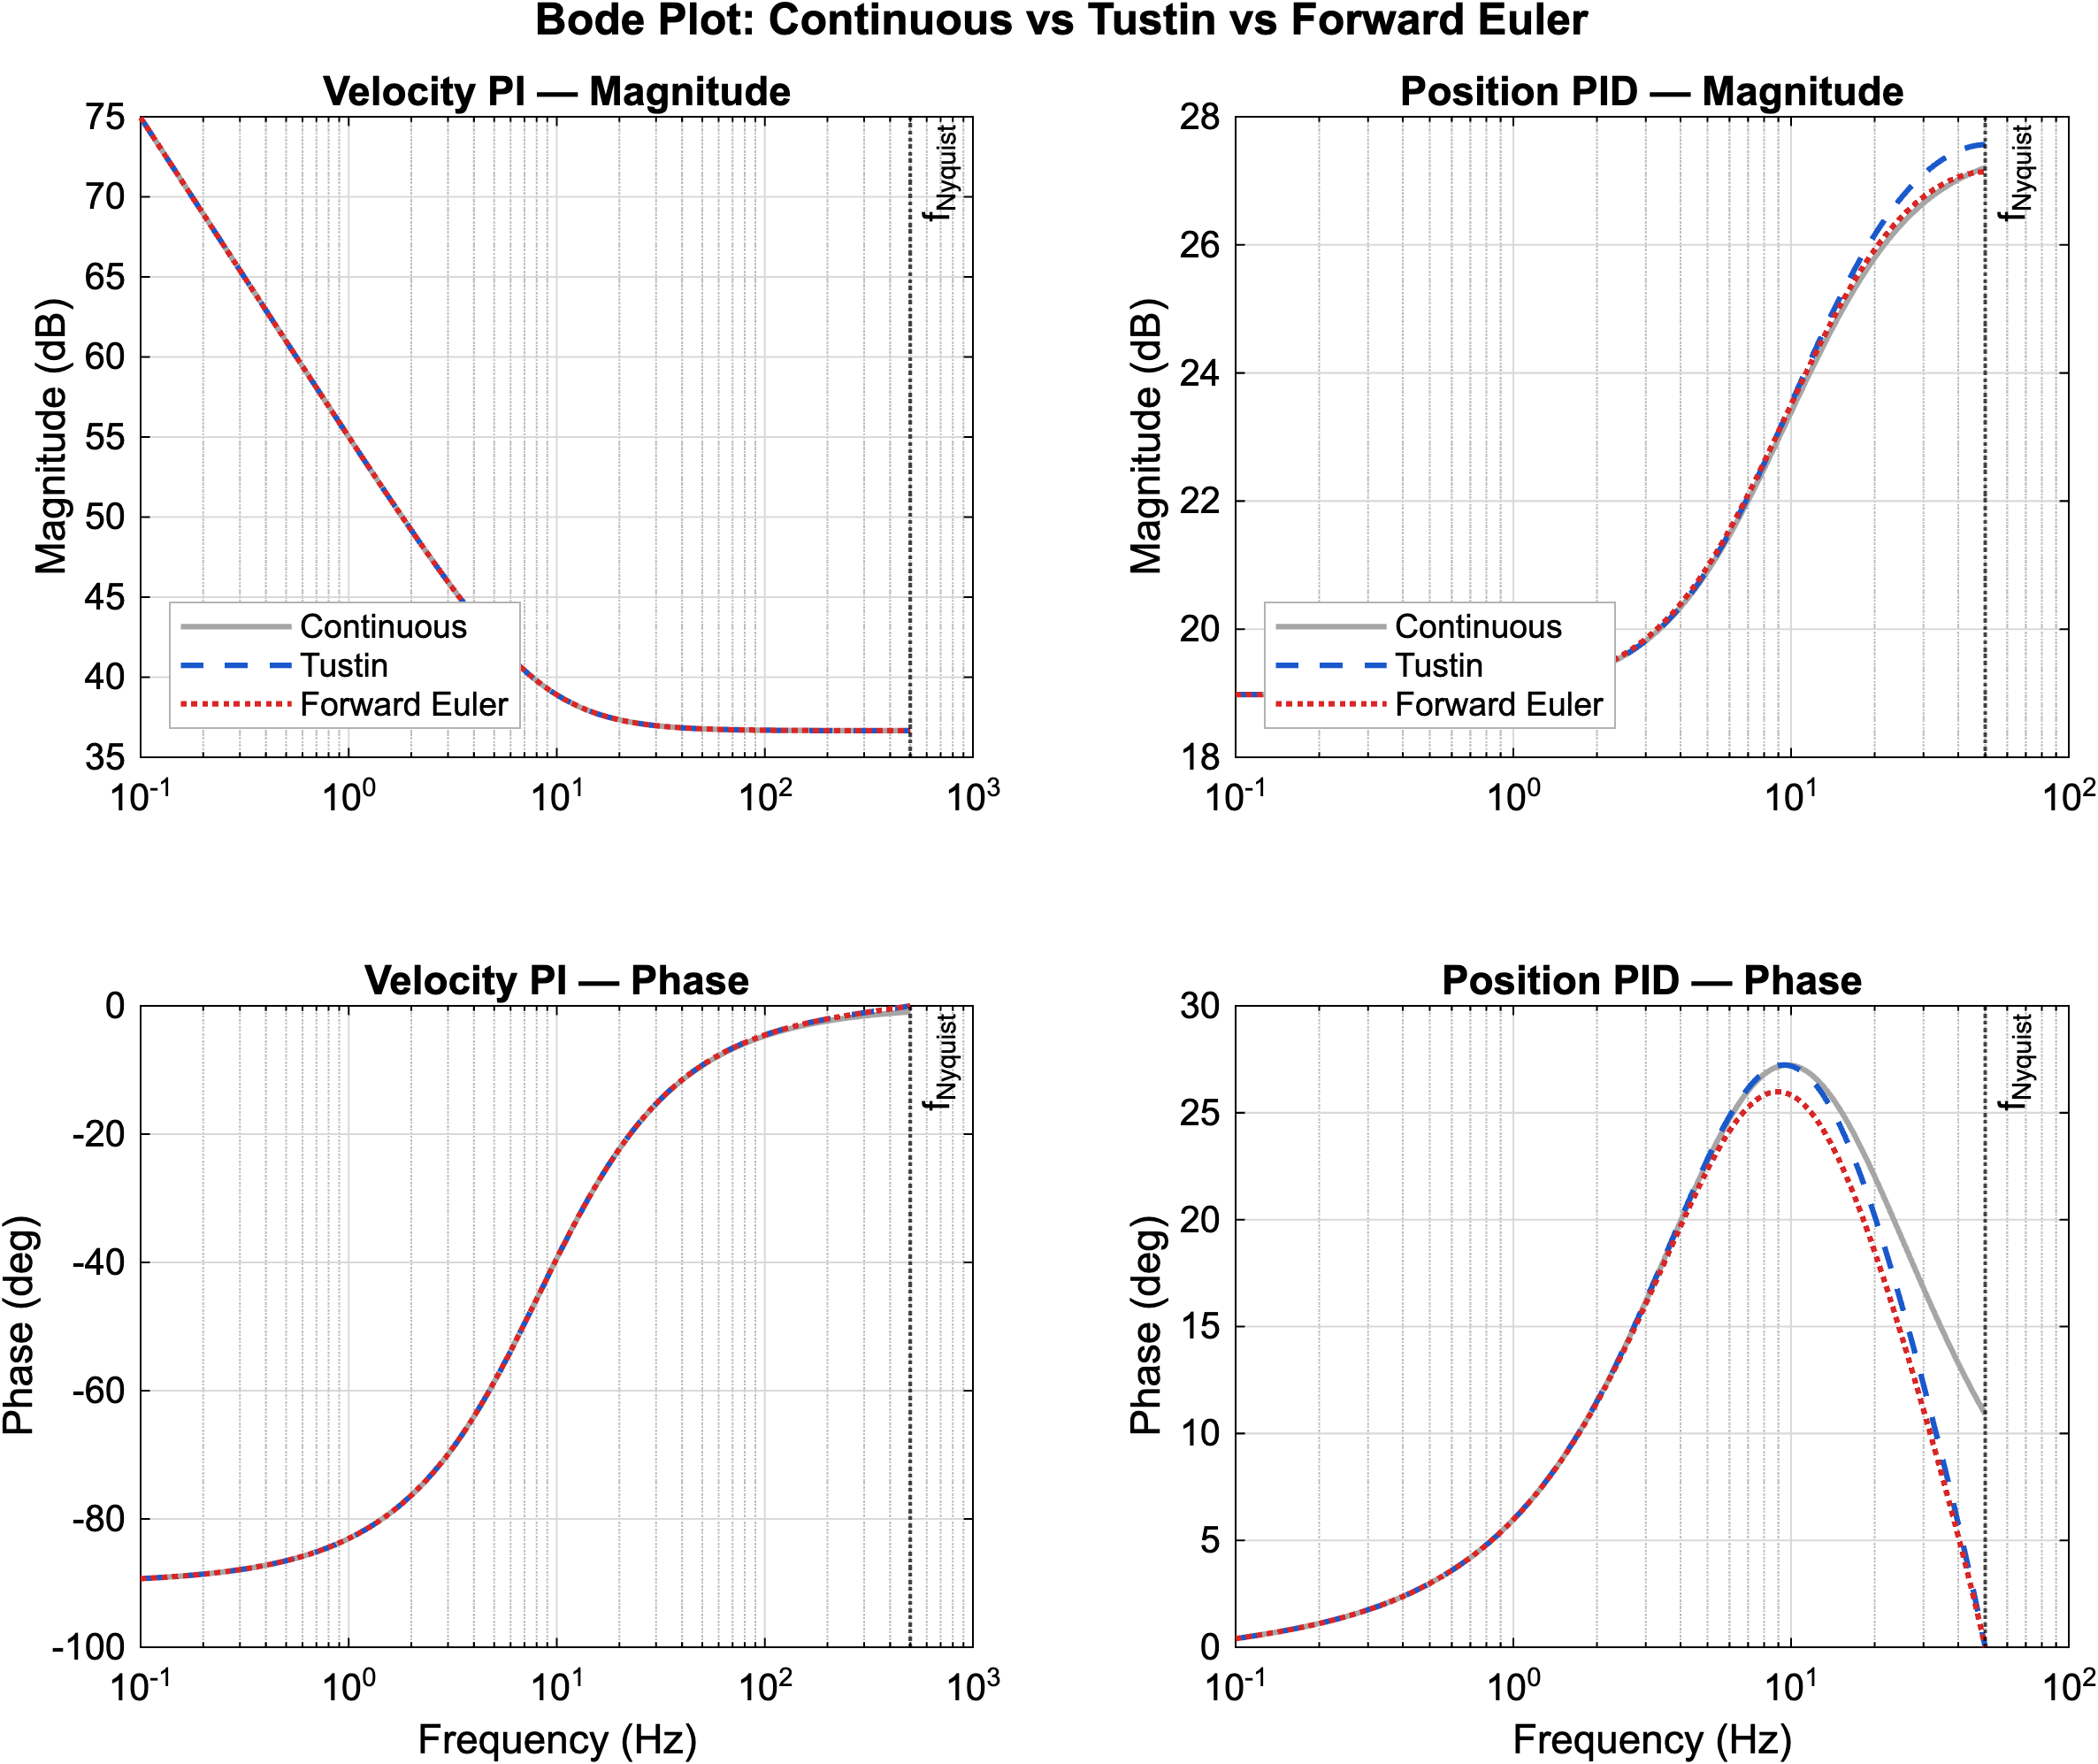
\includegraphics[width=0.90\textwidth]{fig_bode_discretization}
    \caption{Bode Plot เปรียบเทียบ Continuous-time (สีเทา),
             Tustin (สีน้ำเงิน) และ Forward Euler (สีแดง)
             แสดงว่า Tustin ให้ Frequency Response
             ใกล้เคียง Continuous ในย่าน Passband
             ในขณะที่ Forward Euler มี Phase Error
             สูงกว่าเมื่อความถี่เข้าใกล้ $f_{Nyquist}$}
    \label{fig:bode_discretization}
\end{figure}

% -----------------------------------------------------------------------
\subsubsection{การวิเคราะห์เสถียรภาพในโดเมนความถี่}
\label{subsubsec:frequency_analysis}
% -----------------------------------------------------------------------

การวิเคราะห์เสถียรภาพของ Cascade PID ดำเนินการใน
Frequency Domain โดยใช้ Open-loop Bode Plot
เพื่อหา Gain Margin (GM) และ Phase Margin (PM)
ซึ่งเป็น Stability Margin มาตรฐานสำหรับ
Linear Feedback System
เกณฑ์ขั้นต่ำที่ยอมรับได้ทั่วไปคือ
GM $> 6$\,dB และ PM $> 30°$

\begin{figure}[H]
    \centering
    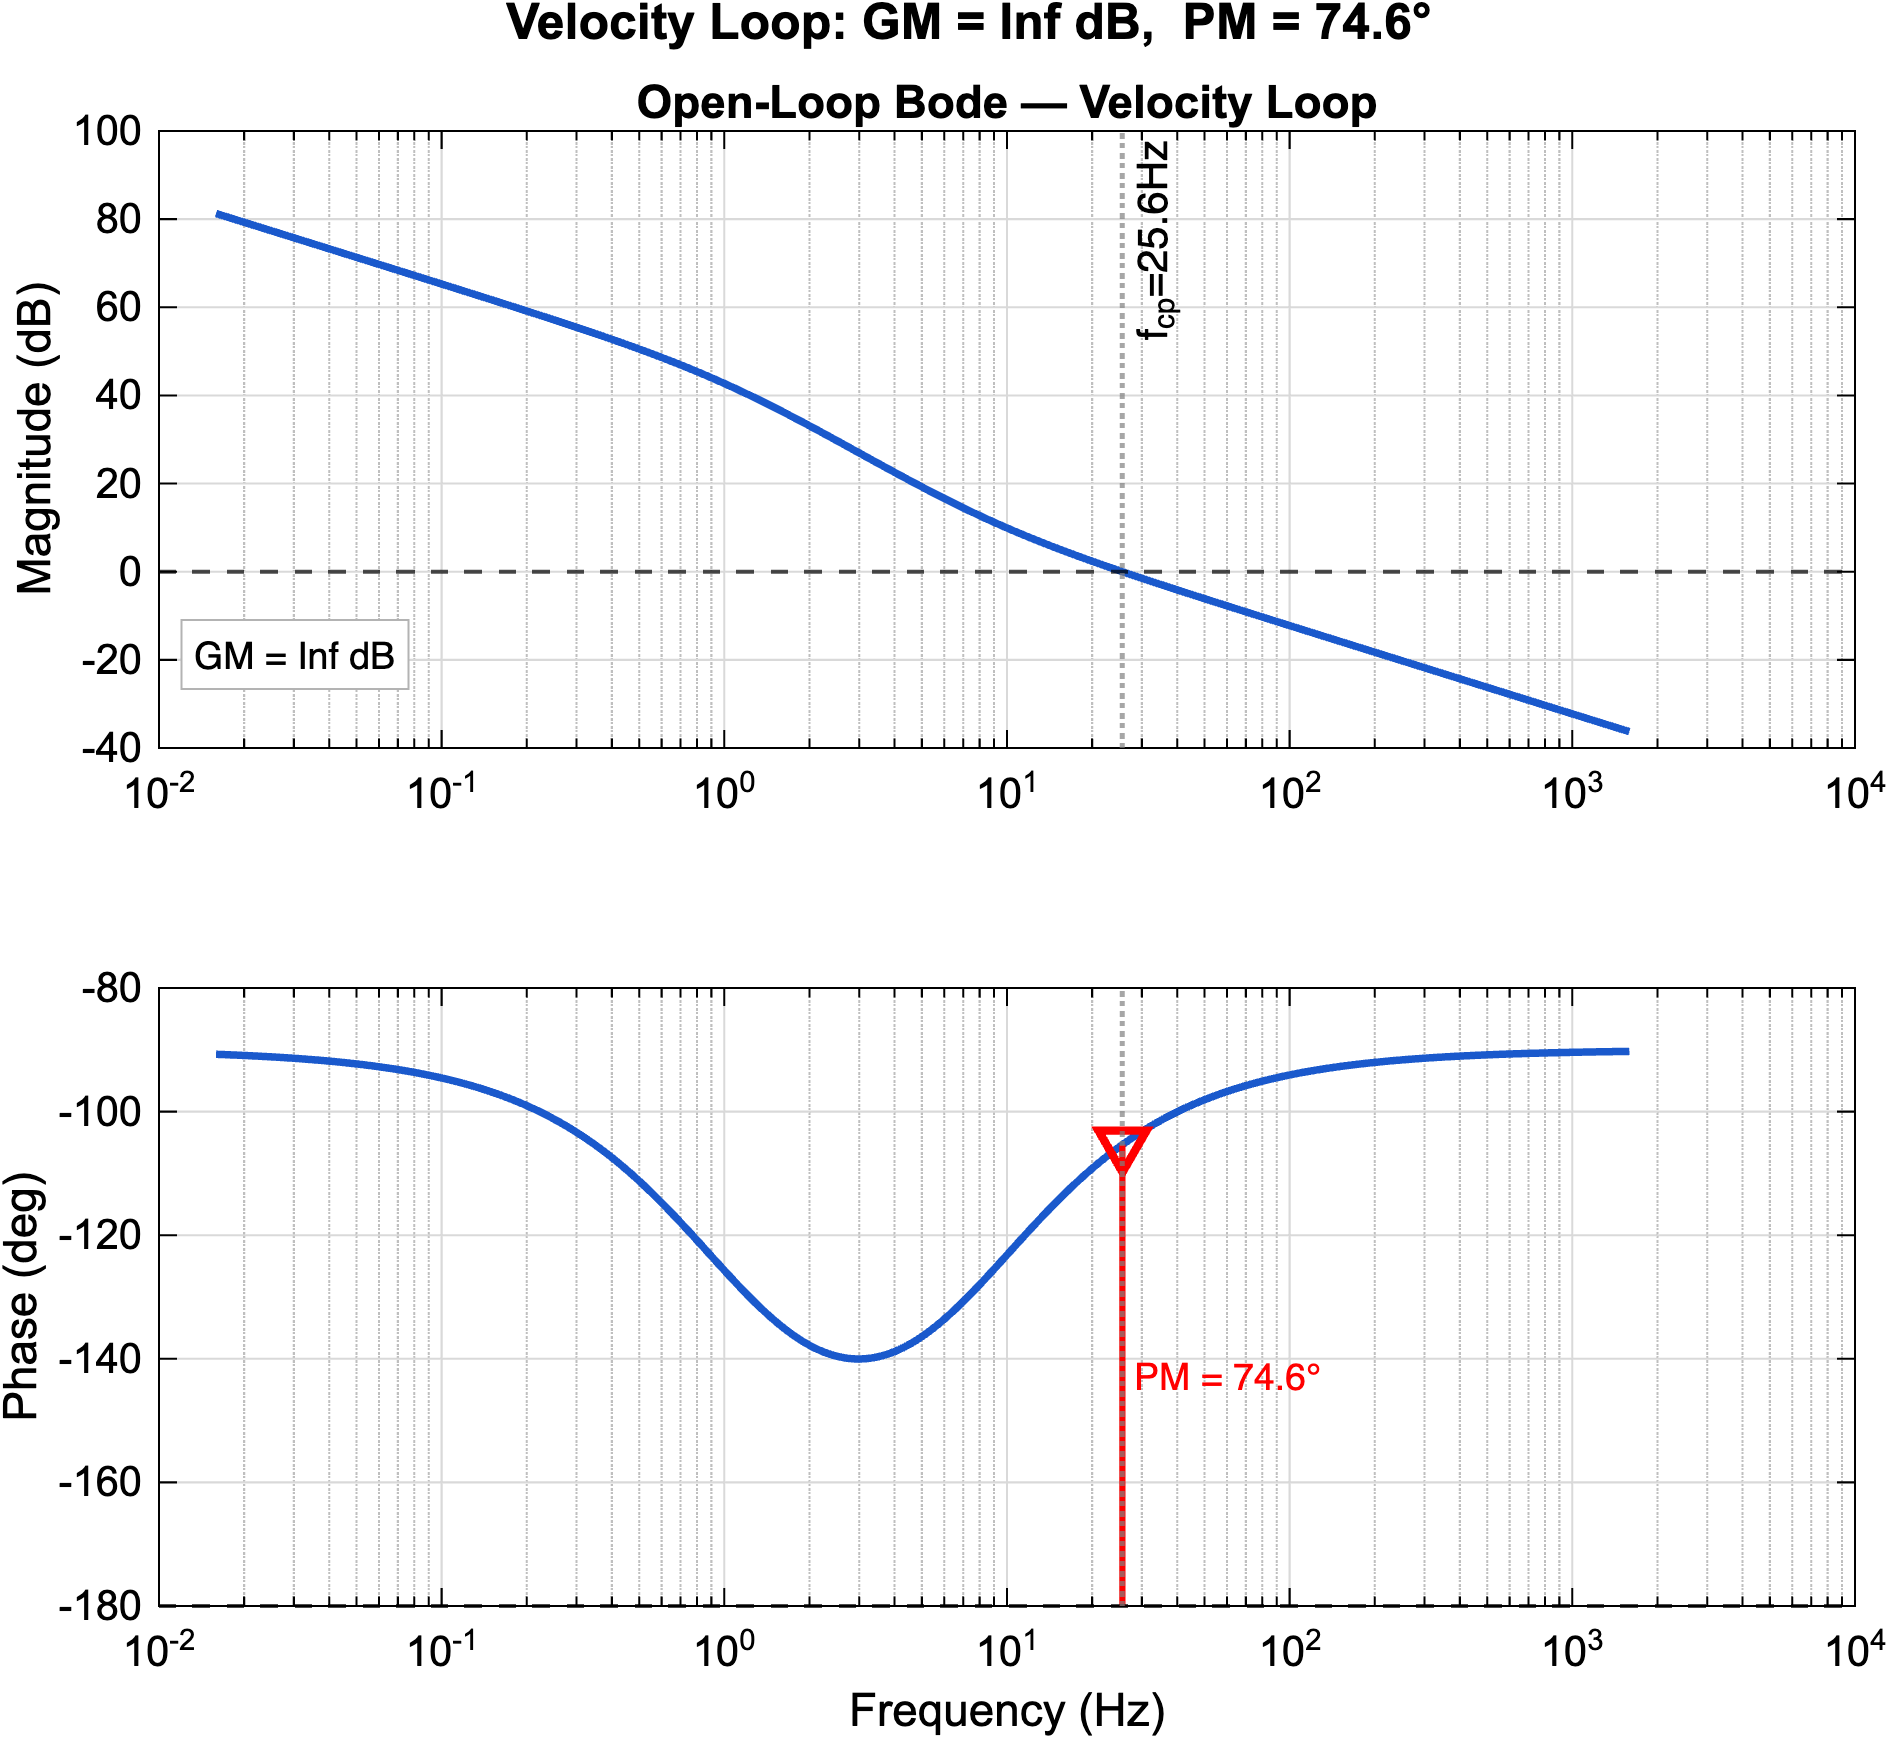
\includegraphics[width=0.85\textwidth]{fig_bode_openloop_vel}
    \caption{Open-Loop Bode Plot ของ Velocity Inner Loop
             แสดง Phase Margin ที่ Gain Crossover Frequency
             ยืนยันความเสถียรของ Velocity Loop}
    \label{fig:bode_openloop_vel}
\end{figure}

\begin{figure}[H]
    \centering
    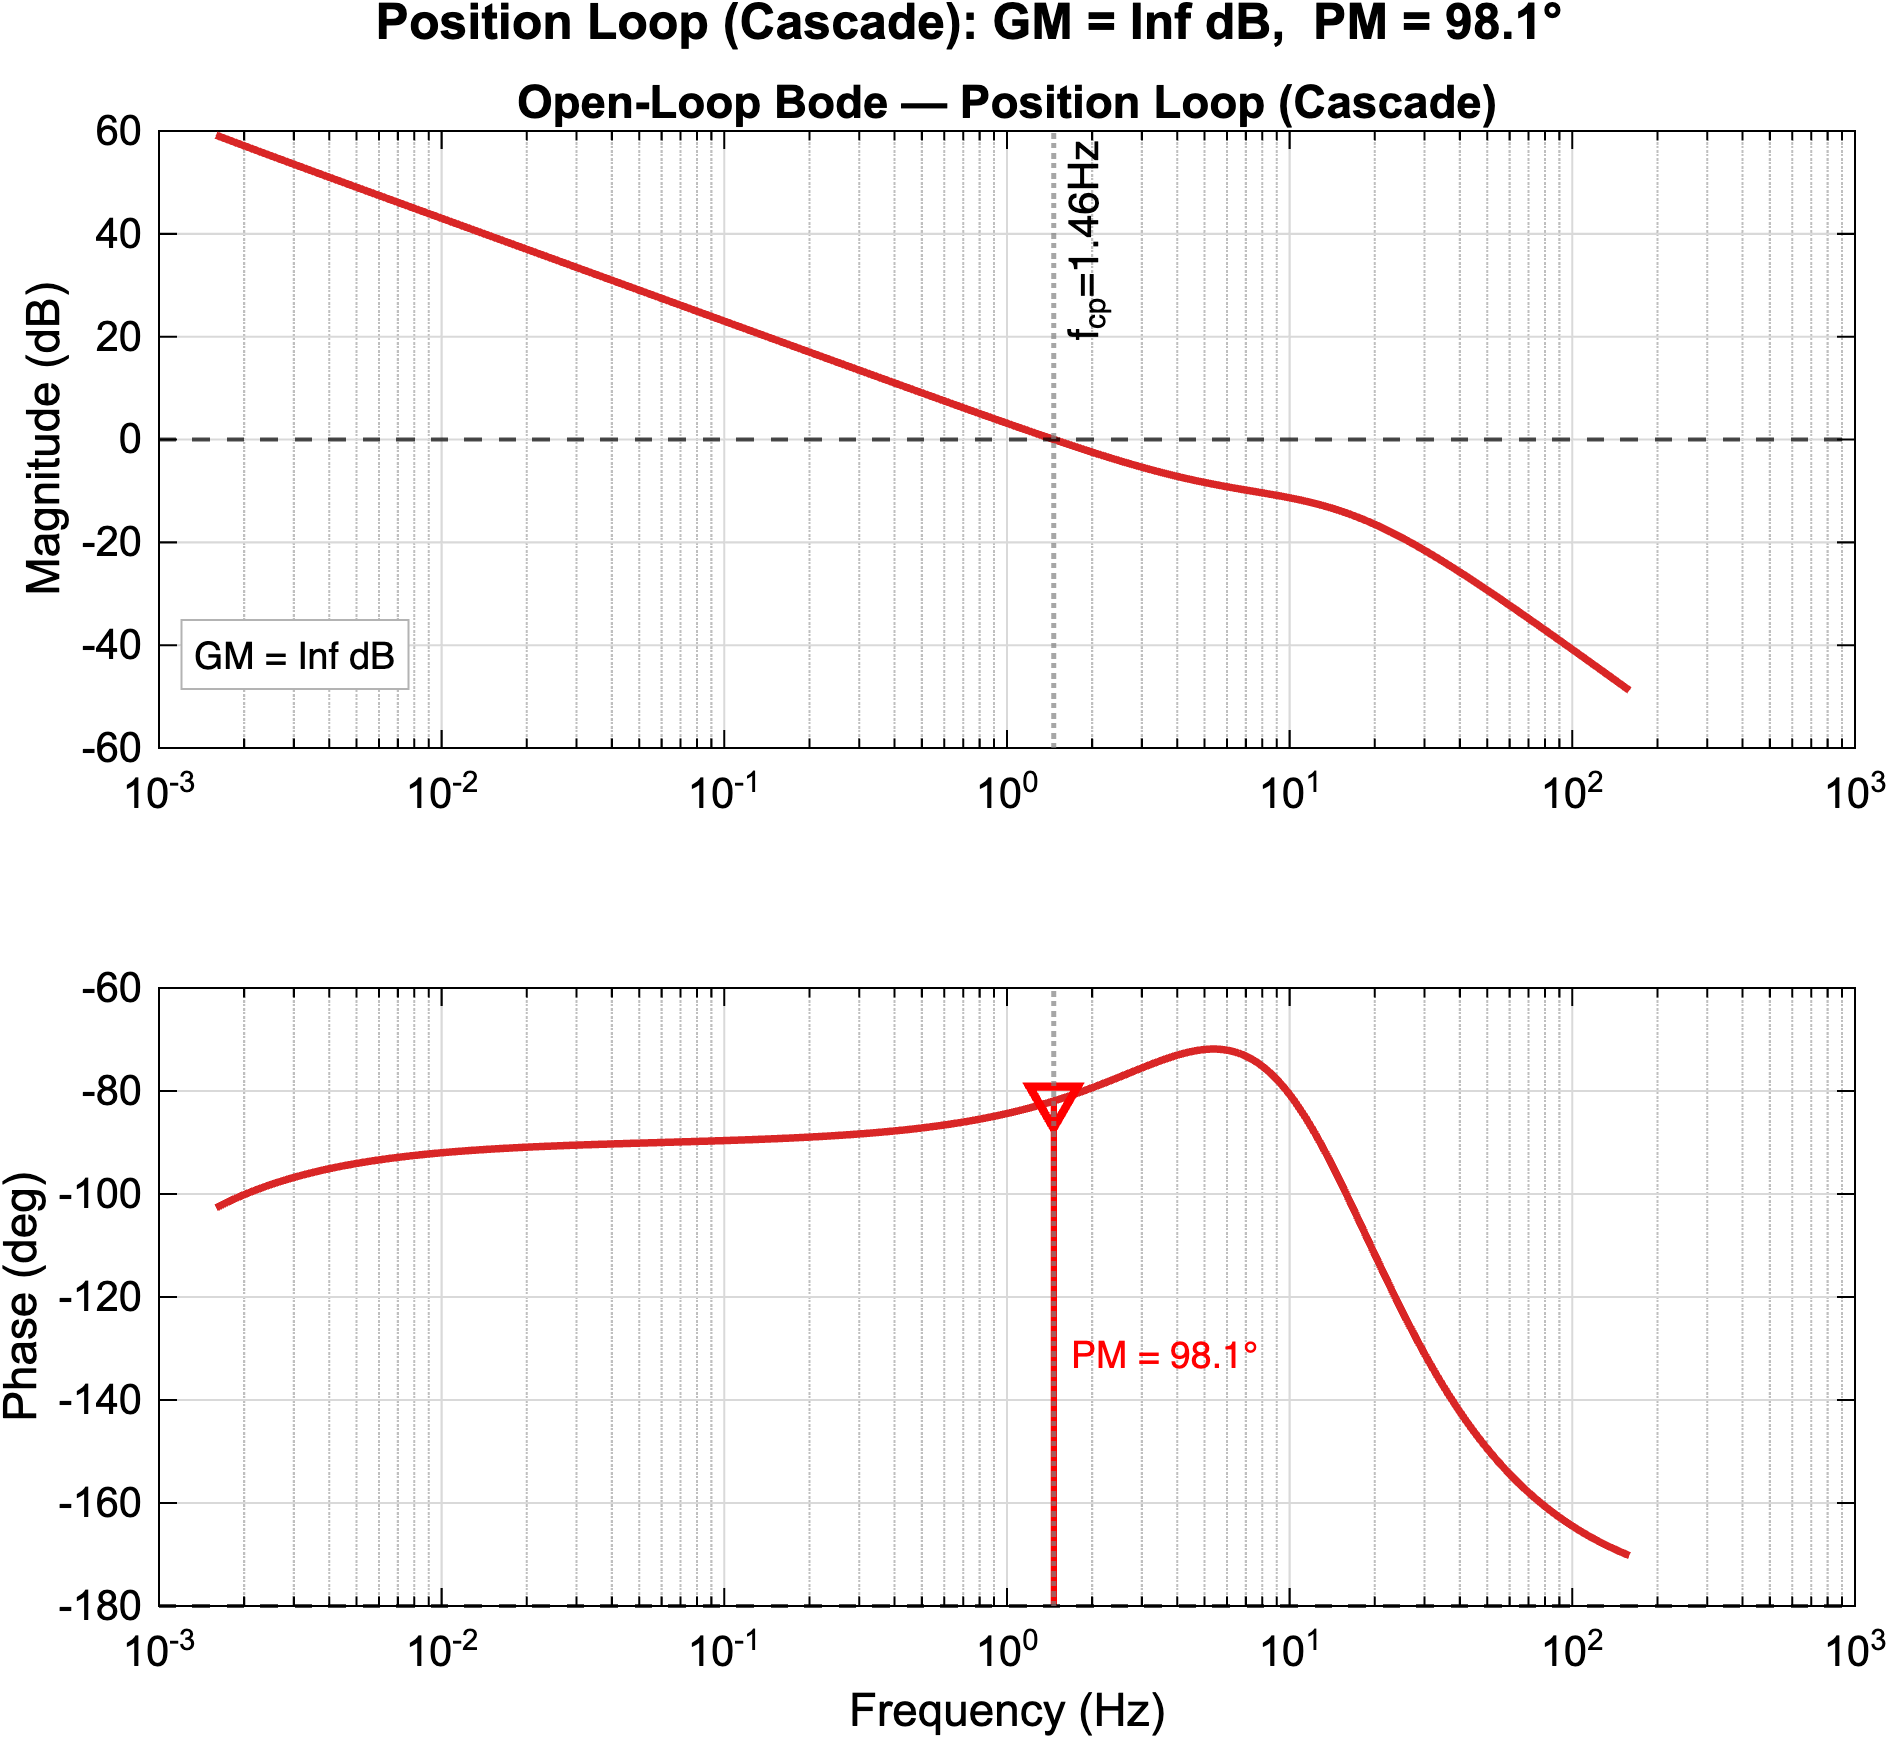
\includegraphics[width=0.85\textwidth]{fig_bode_openloop_pos}
    \caption{Open-Loop Bode Plot ของ Position Outer Loop (Cascade)
             แสดง Gain Margin และ Phase Margin
             ของระบบ Cascade รวมทั้งสอง Loop}
    \label{fig:bode_openloop_pos}
\end{figure}

\begin{table}[H]
  \centering
  \caption{สรุป Stability Margin ของ Cascade PID}
  \label{tab:stability_margin}
  \begin{tabular}{lcccc}
    \toprule
    Loop & GM (dB) & PM (deg) & $f_{cp}$ (Hz) & สถานะ \\
    \midrule
    Velocity Inner & $\infty$ & 74.64 & 25.58 & \textbf{ผ่าน} \\
    Position Outer & $\infty$ & 98.07 &  1.46 & \textbf{ผ่าน} \\
    \bottomrule
    \multicolumn{5}{l}{\small เกณฑ์: GM $> 6$\,dB และ PM $> 30°$} \\
  \end{tabular}
\end{table}

\begin{figure}[H]
    \centering
    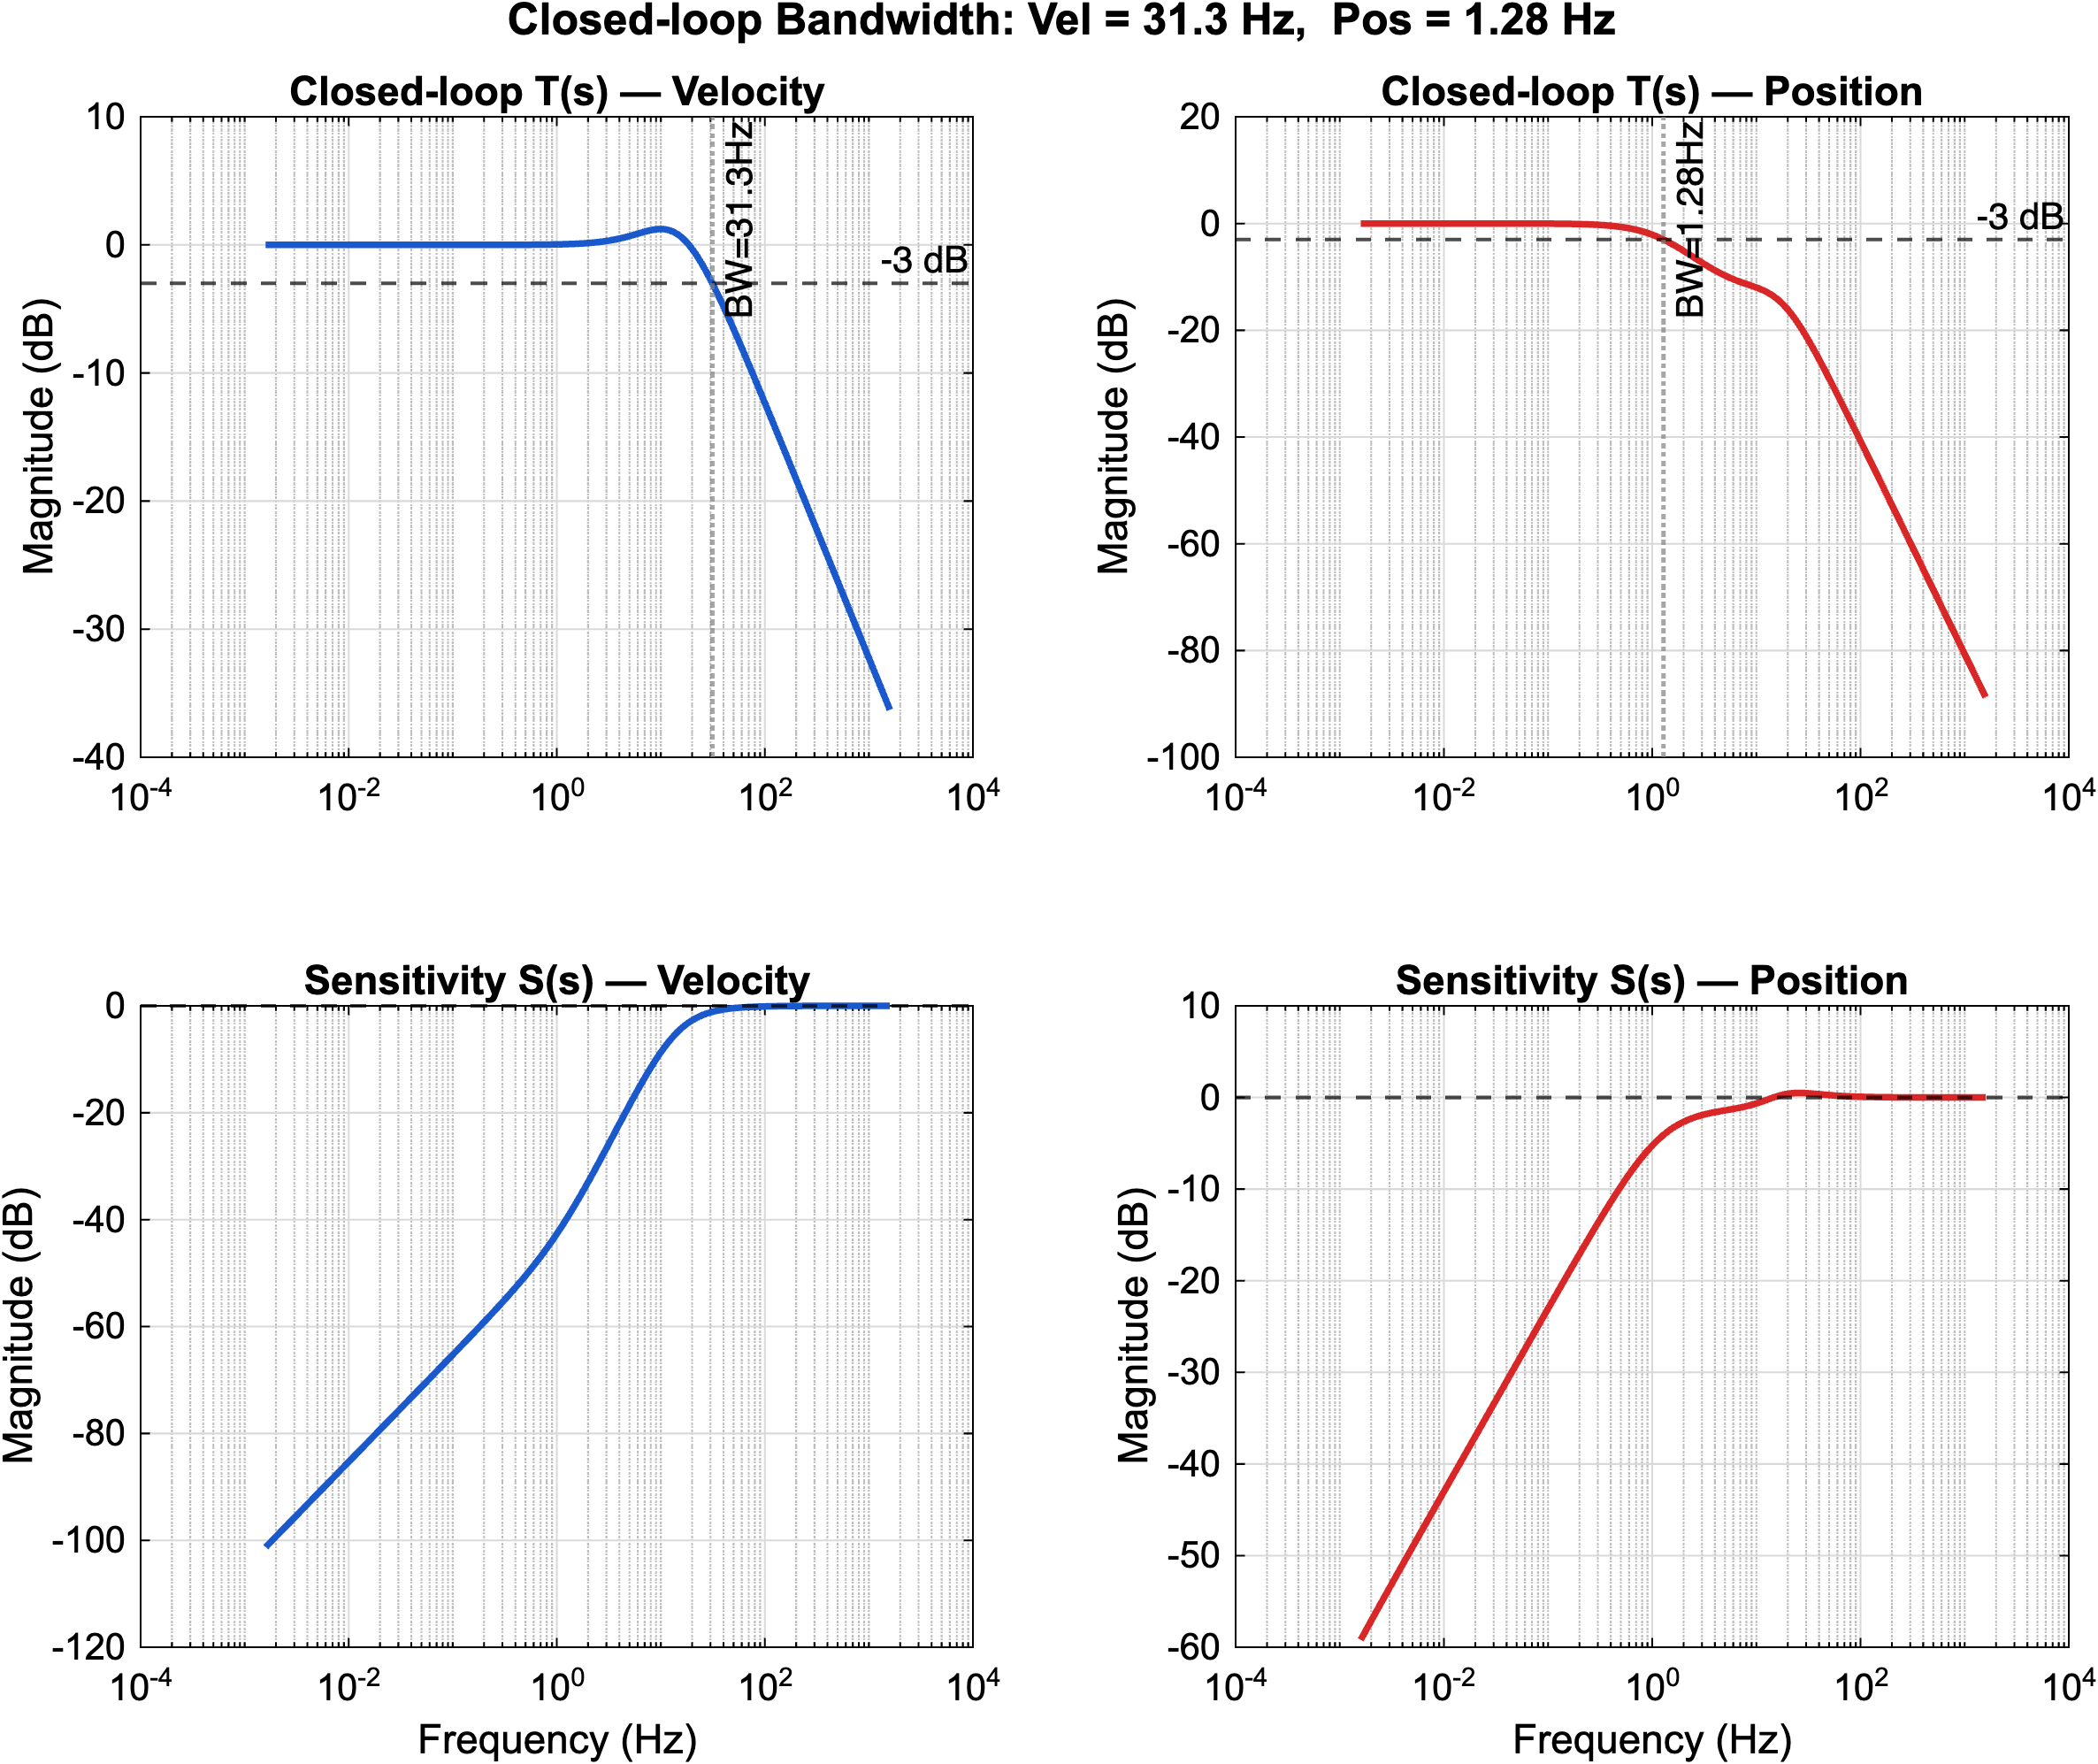
\includegraphics[width=0.90\textwidth]{fig_bode_sensitivity}
    \caption{Closed-loop Frequency Response แสดง
             Complementary Sensitivity $T(s)$ (บน)
             และ Sensitivity $S(s)$ (ล่าง)
             ของ Velocity Loop (ซ้าย) และ Position Loop (ขวา)
             เส้นประแสดงจุด $-3$\,dB Bandwidth ของแต่ละ Loop}
    \label{fig:bode_sensitivity}
\end{figure}

Gain Margin มีค่าเป็น $\infty$ ในทั้งสอง Loop
เนื่องจาก Phase ของ Open-loop Transfer Function
ไม่เคยลดลงถึง $-180°$ ในย่านความถี่ใด
ซึ่งเป็นลักษณะปกติของระบบ PI และ PID
ที่มี Integrator เพียงหนึ่งตัวใน Loop
ดังนั้น Phase Margin จึงเป็น Stability Indicator
หลักของระบบนี้

Phase Margin ของ Velocity Loop ($74.6°$)
และ Position Loop ($98.1°$) สูงกว่าเกณฑ์ขั้นต่ำ
$30°$ อย่างมีนัยสำคัญ
แสดงว่าระบบมี Stability Margin เพียงพอ
และสามารถรองรับ Plant Model Uncertainty
ได้ในระดับสูง

Gain Crossover Frequency ของ Velocity Loop
ที่ $f_{cp} = 25.58$\,Hz ยืนยัน Bandwidth
Separation จาก Position Loop ($f_{cp} = 1.46$\,Hz)
ที่อัตราส่วน $25.58/1.46 \approx 17.5$ เท่า
ซึ่งเกินกว่าเกณฑ์ 10 เท่าที่ออกแบบไว้
ตาม\cref{eq:bw_sep}

% ============================================================================
\subsection{การออกแบบ ZVD Input Shaper}
\label{subsec:zv_design}
% ============================================================================

% -----------------------------------------------------------------------
\subsubsection{แบบจำลอง Connection Rod และเหตุผลที่ต้องใช้ Input Shaping}
\label{subsubsec:rod_model}
% -----------------------------------------------------------------------

Connection Rod มีมวล $m_{rod} = 164.08$\,g และความยาว $L_{rod} = 100$\,mm
จำลองเป็น Simple Pendulum ที่ถูกกระตุ้นด้วย Angular Acceleration
ของแขนกล $\alpha_{arm}$ ตามที่อธิบายใน\cref{subsec:rod_dynamics}
สมการการเคลื่อนที่ในรูปแบบ Standard 2nd-order ได้จาก\cref{eq:rod_eom}

\begin{equation}
    \ddot{\phi} + 2\zeta_{rod}\,\omega_{n,rod}\,\dot{\phi}
    + \omega_{n,rod}^2\,\phi
    = \underbrace{-\frac{3\,r_{arm}}{2\,L_{rod}}}_{\Gamma}\,\alpha_{arm}
    \label{eq:rod_eom_ch3}
\end{equation}

\noindent โดยที่ $\Gamma = -3 \times 0.5 / (2 \times 0.1) = -7.5$
คือ Forcing Gain และความถี่ธรรมชาติคำนวณได้จาก\cref{eq:rod_natural_freq}

\begin{equation}
    \omega_{n,rod} = \sqrt{\frac{3g}{2L_{rod}}}
                   = \sqrt{\frac{3 \times 9.81}{2 \times 0.1}}
                   = 12.131\,\text{rad/s}
                   \quad (f_n = 1.931\,\text{Hz})
    \label{eq:rod_wn_ch3}
\end{equation}

ค่า Damping Ratio $\zeta_{rod} = 0.041$ ใช้เป็น Conservative Assumption
สำหรับ Lightly Damped Mechanical System
ซึ่งให้ Settling Time ต่อ Move ที่

\begin{equation}
    t_{settle,rod} \approx \frac{4}{\zeta_{rod}\,\omega_{n,rod}}
                         = \frac{4}{0.041 \times 12.131}
                         = 8.04\,\text{s/move}
    \label{eq:rod_settle}
\end{equation}

หากระบบมี 9 Moves ต่อ Cycle และต้องรอให้ Rod หยุดแกว่งก่อนทุก Move
Cycle Time รวมจะเกิน $9 \times 8.04 = 72.4$\,s
ซึ่งเกินข้อกำหนด P1 ($\leq 35$\,s) อย่างมาก
การใช้ Input Shaper จึงเป็นข้อกำหนดที่ขาดไม่ได้

% -----------------------------------------------------------------------
\subsubsection{การออกแบบ ZVD Input Shaper (3-Impulse)}
\label{subsubsec:zvd_design}
% -----------------------------------------------------------------------

ระบบเลือกใช้ ZVD (Zero-Vibration-Derivative) Shaper แบบ 3-Impulse
แทน ZV แบบ 2-Impulse เนื่องจาก ZVD มีเงื่อนไขเพิ่มเติม
ว่า Derivative ของ Residual Vibration เทียบกับ $\omega_n$
ต้องเป็นศูนย์ด้วย ทำให้ทนทานต่อความไม่แน่นอนของ $\omega_n$
ได้สูงกว่า ดังที่จะเห็นใน\cref{fig:zvd_sensitivity}

\paragraph{การคำนวณพารามิเตอร์ ZVD}

กำหนดค่า Decay Factor

\begin{equation}
    K = e^{-\zeta_{rod}\pi/\sqrt{1-\zeta_{rod}^2}}
      = e^{-0.041\pi/\sqrt{1-0.041^2}}
      = e^{-0.1288}
      = 0.8790
    \label{eq:zvd_K}
\end{equation}

แอมพลิจูดของ Impulse ทั้งสามคำนวณจาก\cref{eq:zv_amplitudes}

\begin{align}
    A_1 &= \frac{1}{(1+K)^2}
         = \frac{1}{(1.8790)^2}
         = 0.2832
    \label{eq:zvd_A1} \\[4pt]
    A_2 &= \frac{2K}{(1+K)^2}
         = \frac{2 \times 0.8790}{(1.8790)^2}
         = 0.4979
    \label{eq:zvd_A2} \\[4pt]
    A_3 &= \frac{K^2}{(1+K)^2}
         = \frac{(0.8790)^2}{(1.8790)^2}
         = 0.2189
    \label{eq:zvd_A3}
\end{align}

ตรวจสอบ: $A_1 + A_2 + A_3 = 0.2832 + 0.4979 + 0.2189 = 1.0000$ \checkmark

Impulse Delay คำนวณจาก Half-Period ของ Damped Oscillation

\begin{equation}
    T_d = \frac{\pi}{\omega_{n,rod}\sqrt{1-\zeta_{rod}^2}}
        = \frac{\pi}{12.131 \times \sqrt{1-0.041^2}}
        = \frac{\pi}{12.121}
        = 0.2592\,\text{s}
    \label{eq:zvd_Td}
\end{equation}

\begin{equation}
    t_2 = T_d = 0.2592\,\text{s}
    \quad (26\;\text{steps @ 100\,Hz}),
    \qquad
    t_3 = 2T_d = 0.5184\,\text{s}
    \quad (52\;\text{steps @ 100\,Hz})
    \label{eq:zvd_delays}
\end{equation}

% -----------------------------------------------------------------------
% รูปที่: ZVD Impulse Sequence
% ชื่อไฟล์: fig_zvd_impulse_sequence.png
% -----------------------------------------------------------------------
\begin{figure}[H]
    \centering
    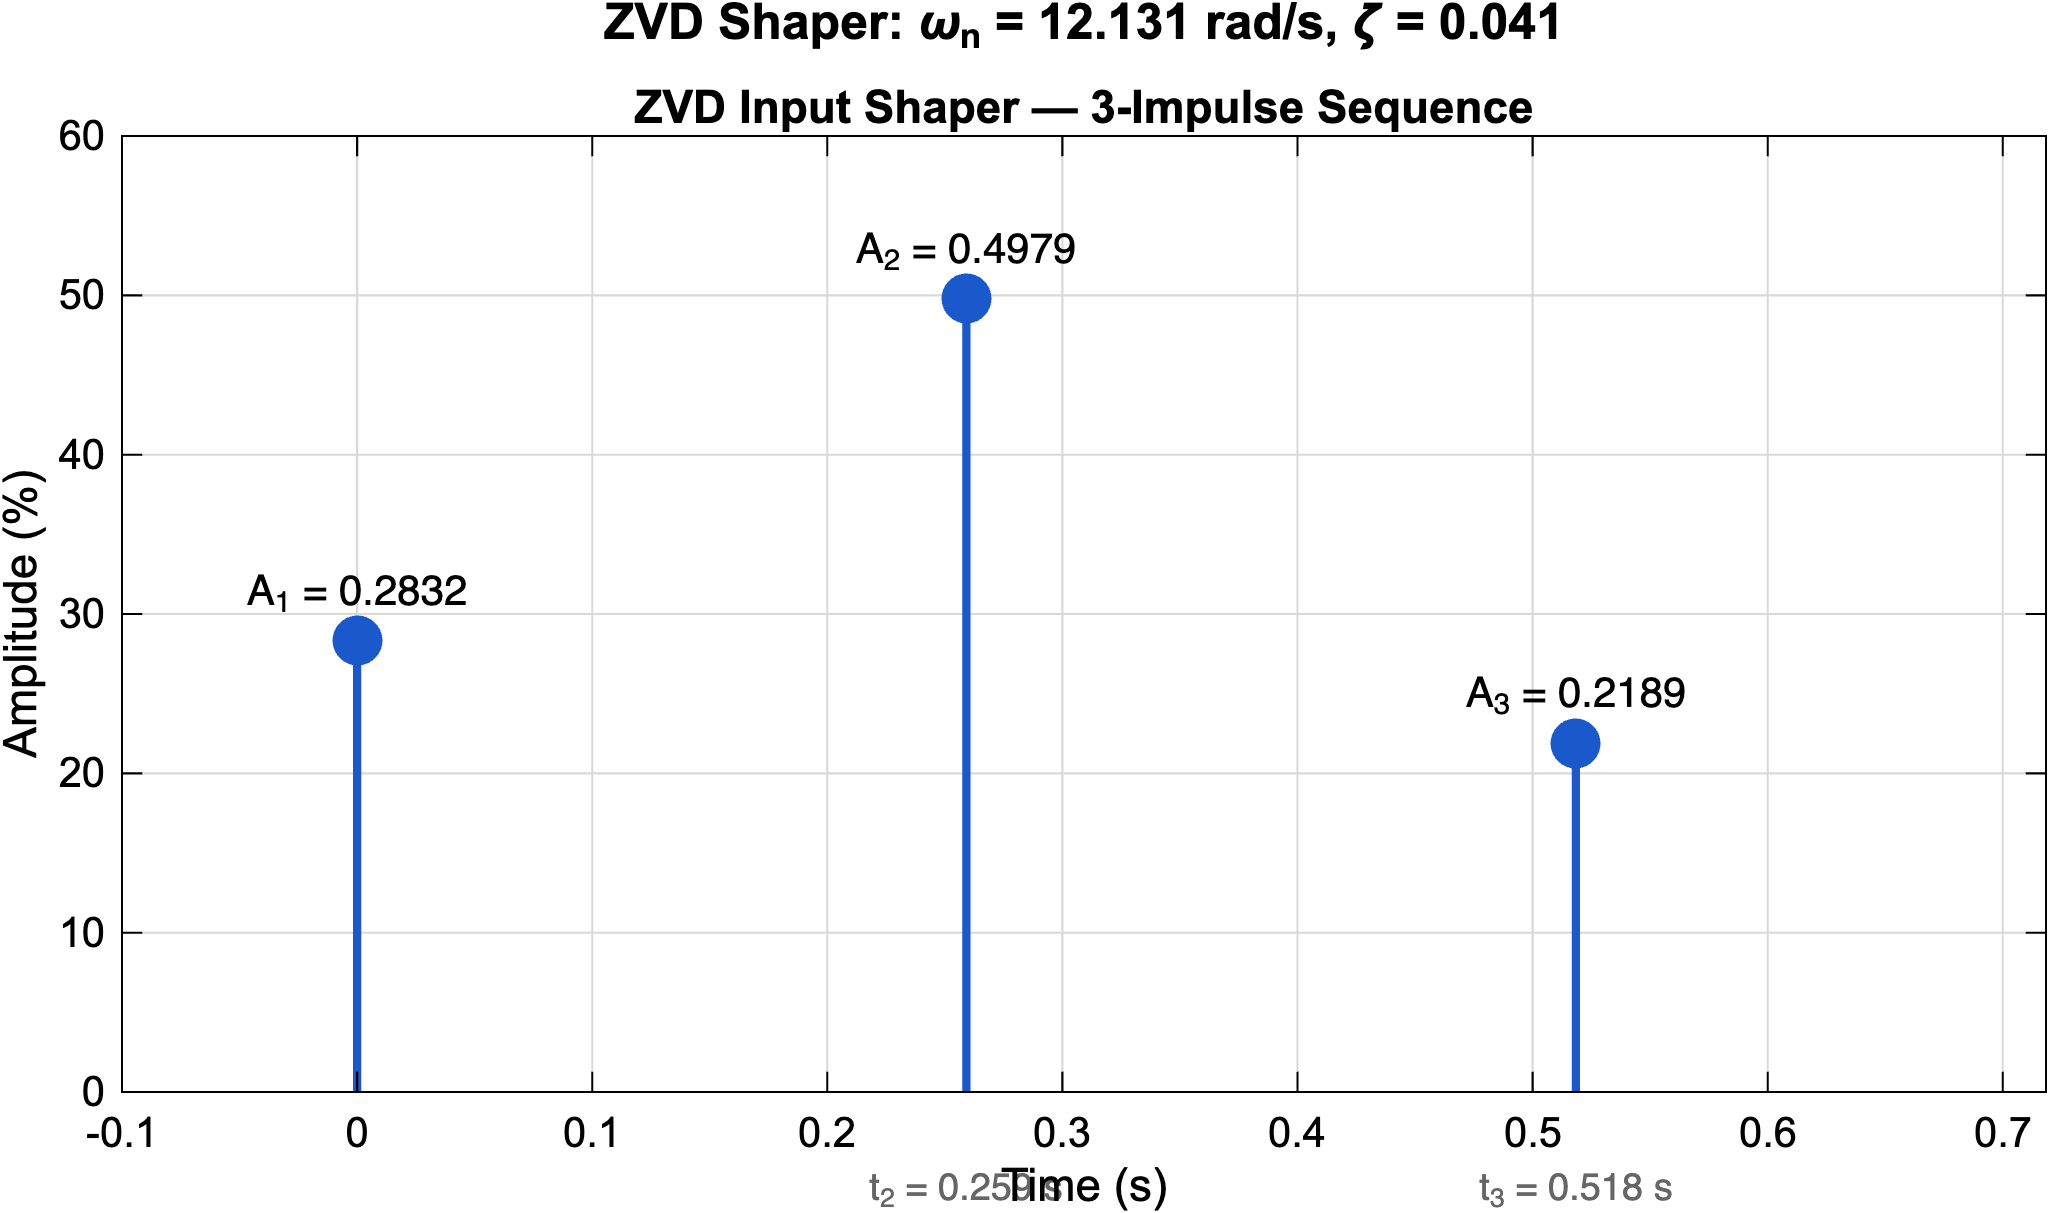
\includegraphics[width=0.75\textwidth]{fig_zvd_impulse_sequence}
    \caption{ZVD 3-Impulse Sequence แสดงแอมพลิจูด $A_1$, $A_2$, $A_3$
             และเวลาหน่วง $t_2 = 0.259$\,s ($26$ steps)
             และ $t_3 = 0.518$\,s ($52$ steps) ที่ Outer Loop 100\,Hz}
    \label{fig:zvd_impulse_sequence}
\end{figure}

\begin{table}[H]
  \centering
  \caption{พารามิเตอร์ ZVD Input Shaper ที่ใช้ใน Firmware}
  \label{tab:zvd_params}
  \begin{tabular}{llll}
    \toprule
    พารามิเตอร์ & สัญลักษณ์ & ค่า & หมายเหตุ \\
    \midrule
    Natural Frequency & $\omega_{n,rod}$ & 12.131\,rad/s & คำนวณจาก\cref{eq:rod_wn_ch3} \\
    Damping Ratio     & $\zeta_{rod}$    & 0.041         & Conservative Assumption \\
    Decay Factor      & $K$              & 0.8790        & \cref{eq:zvd_K} \\
    Impulse 1         & $A_1$            & 0.2832        & \cref{eq:zvd_A1} \\
    Impulse 2         & $A_2$            & 0.4979        & \cref{eq:zvd_A2} \\
    Impulse 3         & $A_3$            & 0.2189        & \cref{eq:zvd_A3} \\
    Delay 2           & $t_2$            & 0.2592\,s (26 steps) & \cref{eq:zvd_delays} \\
    Delay 3           & $t_3$            & 0.5184\,s (52 steps) & \cref{eq:zvd_delays} \\
    \bottomrule
  \end{tabular}
\end{table}

% -----------------------------------------------------------------------
\subsubsection{การวิเคราะห์ความทนทานต่อความไม่แน่นอนของความถี่}
\label{subsubsec:zvd_sensitivity}
% -----------------------------------------------------------------------

ในการใช้งานจริง ค่า $\omega_{n,rod}$ อาจเปลี่ยนแปลงได้
เนื่องจากน้ำหนักของ Connection Rod ที่แตกต่างกัน
หรือความยาวของ Rod ที่ไม่แน่นอน
\cref{fig:zvd_sensitivity} แสดง Residual Vibration
เมื่อ $\omega_{actual}$ ต่างจาก $\omega_{design}$
สำหรับ ZV (2-Impulse) และ ZVD (3-Impulse)

% -----------------------------------------------------------------------
% รูปที่: ZVD Sensitivity Analysis
% ชื่อไฟล์: fig_zvd_sensitivity.png
% -----------------------------------------------------------------------
\begin{figure}[H]
    \centering
    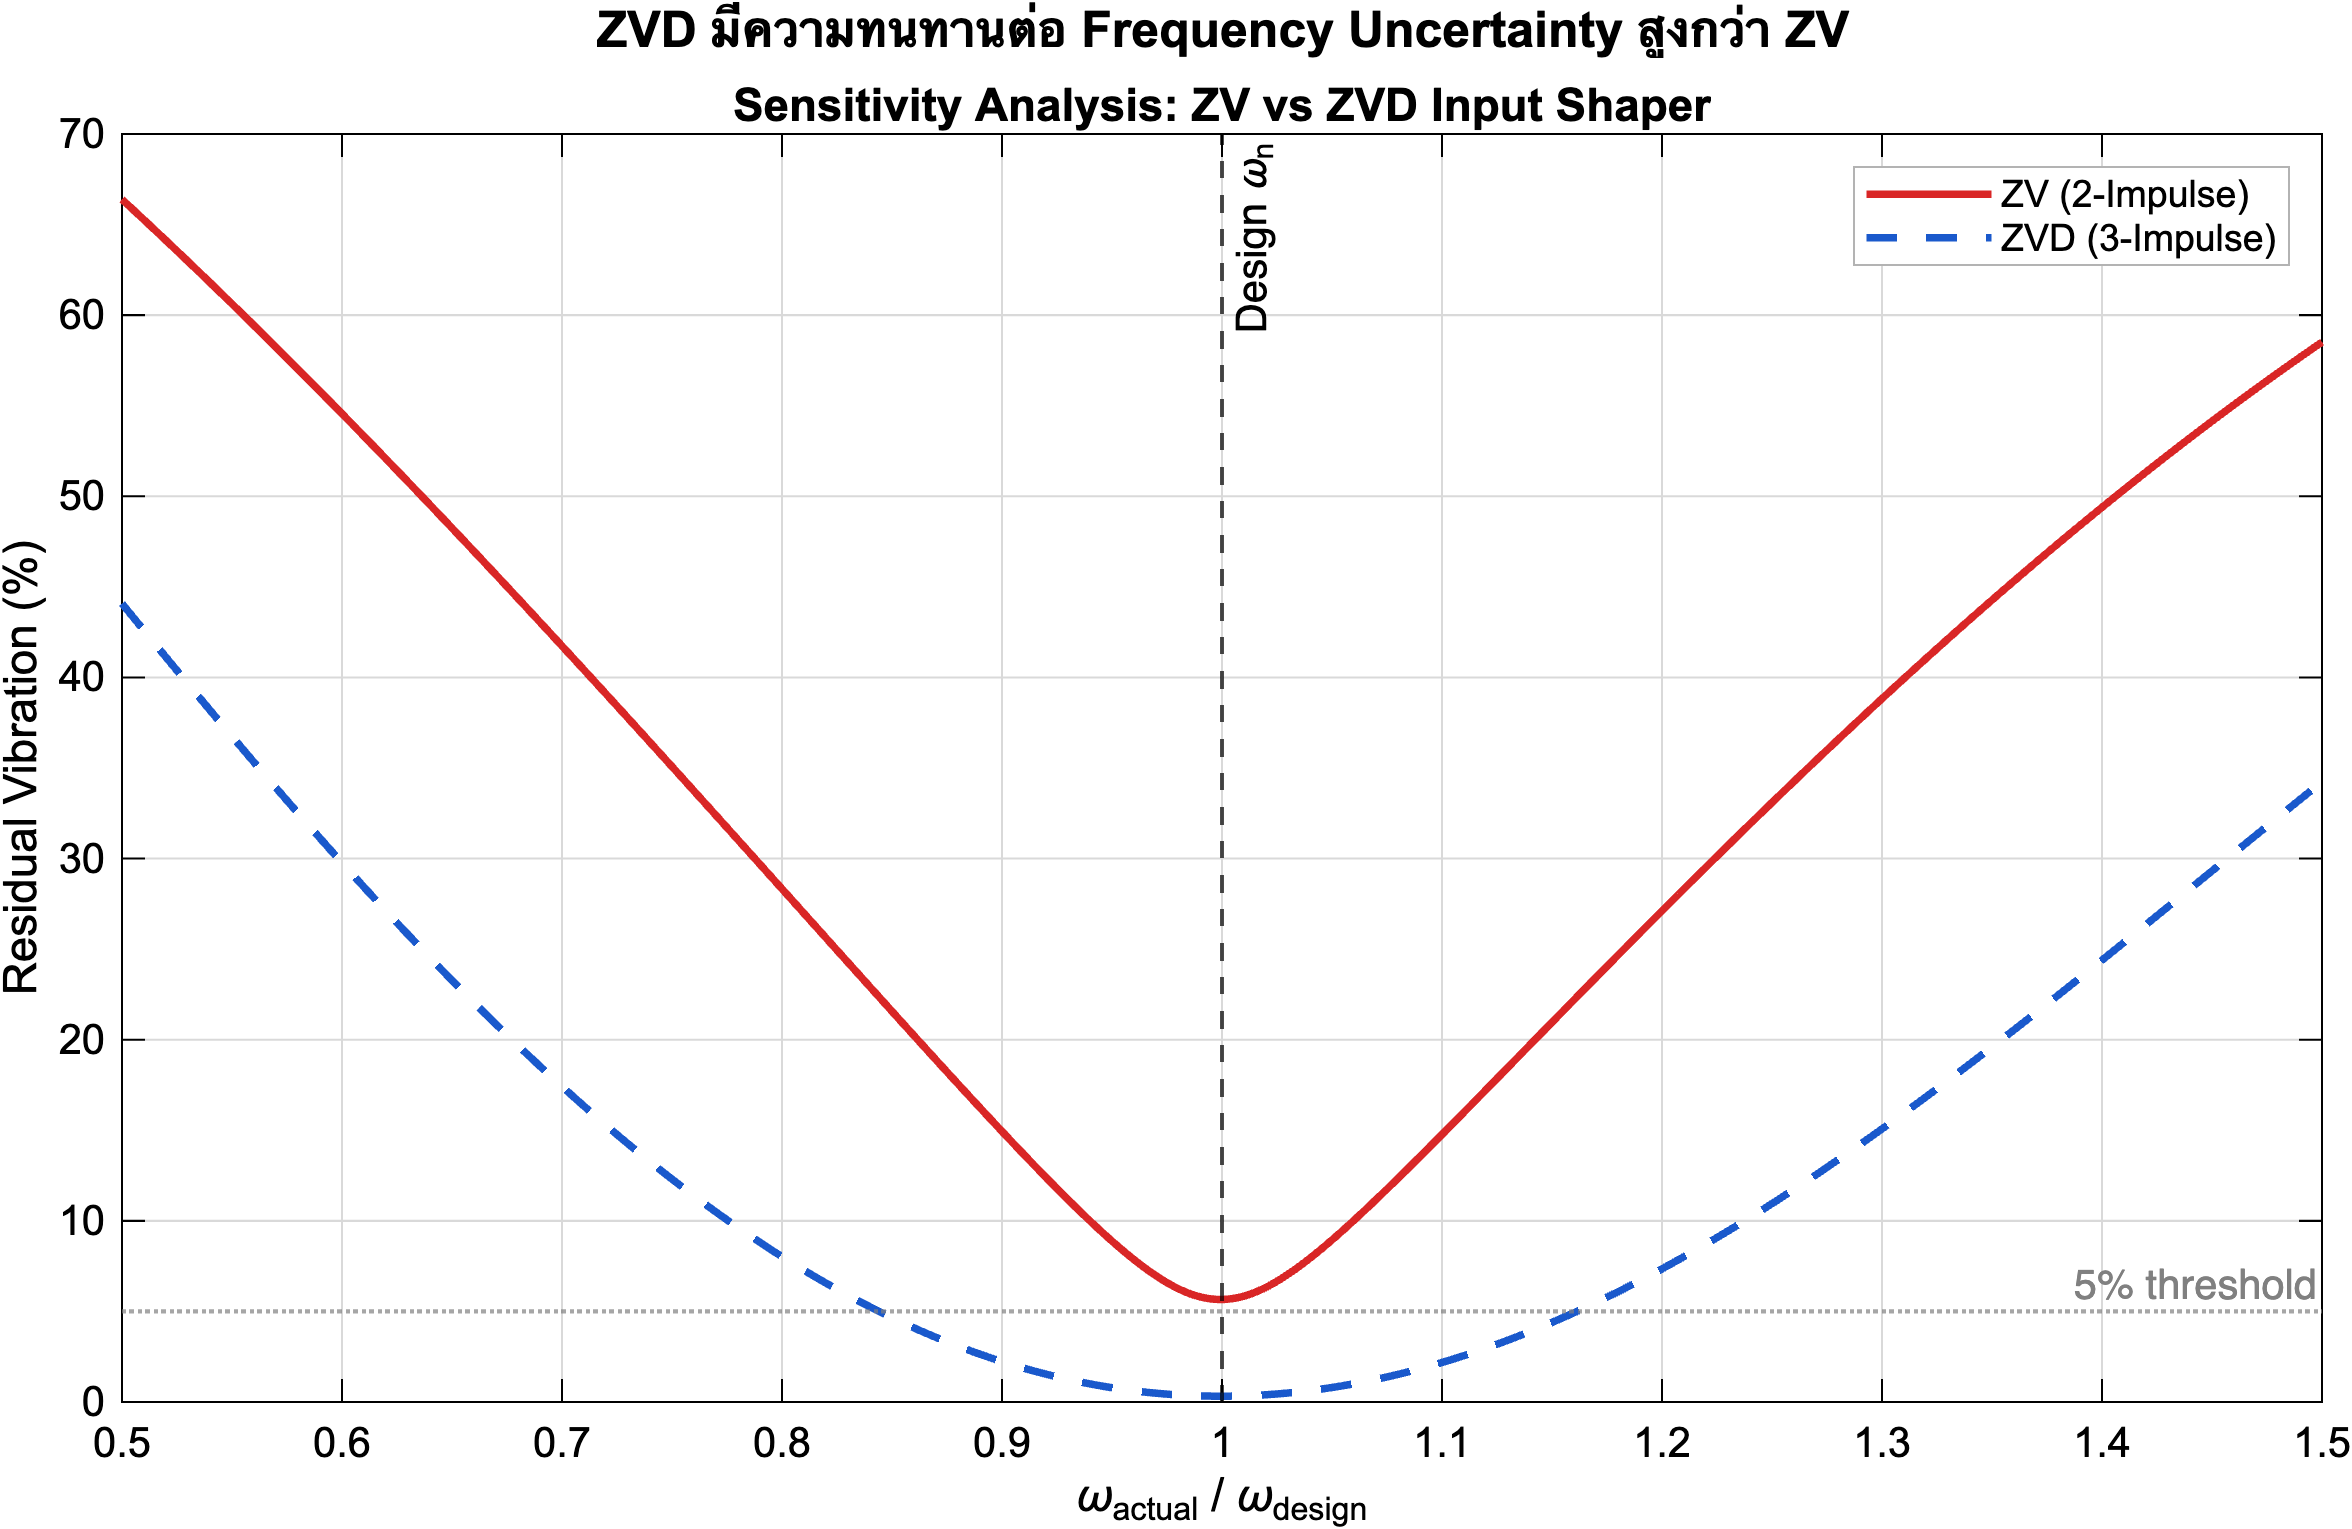
\includegraphics[width=0.82\textwidth]{fig_zvd_sensitivity}
    \caption{Sensitivity Analysis เปรียบเทียบ ZV (สีแดง)
             และ ZVD (สีน้ำเงิน) แสดง Residual Vibration
             เมื่อ $\omega_{actual}/\omega_{design}$ เบี่ยงจาก 1.0
             ZVD รักษา Residual Vibration ต่ำกว่า 5\%
             ในย่านกว้างกว่า ZV อย่างมีนัยสำคัญ}
    \label{fig:zvd_sensitivity}
\end{figure}

จากกราฟ ZVD รักษา Residual Vibration ต่ำกว่า 5\%
ในย่าน $\omega_{actual}/\omega_{design} \in [0.88, 1.12]$
ในขณะที่ ZV รักษาได้เพียง $[0.94, 1.06]$
แสดงว่า ZVD ทนทานต่อความไม่แน่นอนของ $\omega_n$
ได้กว้างกว่าประมาณ 2 เท่า

% -----------------------------------------------------------------------
\subsubsection{ผลการ Simulation: Unshaped กับ ZVD-Shaped}
\label{subsubsec:zvd_results}
% -----------------------------------------------------------------------

\cref{fig:zvd_rod_response} แสดงผลการ Simulation
ของการแกว่ง Rod ในสภาวะ Worst-case
(Move 360° ด้วย S-curve ที่ $v_{max} = 7.304$\,rad/s,
$a_{max} = 27.49$\,rad/s$^2$, $j_{max} = 1400$\,rad/s$^3$)

% -----------------------------------------------------------------------
% รูปที่: Rod Swing Response
% ชื่อไฟล์: fig_zvd_rod_response.png
% -----------------------------------------------------------------------
\begin{figure}[H]
    \centering
    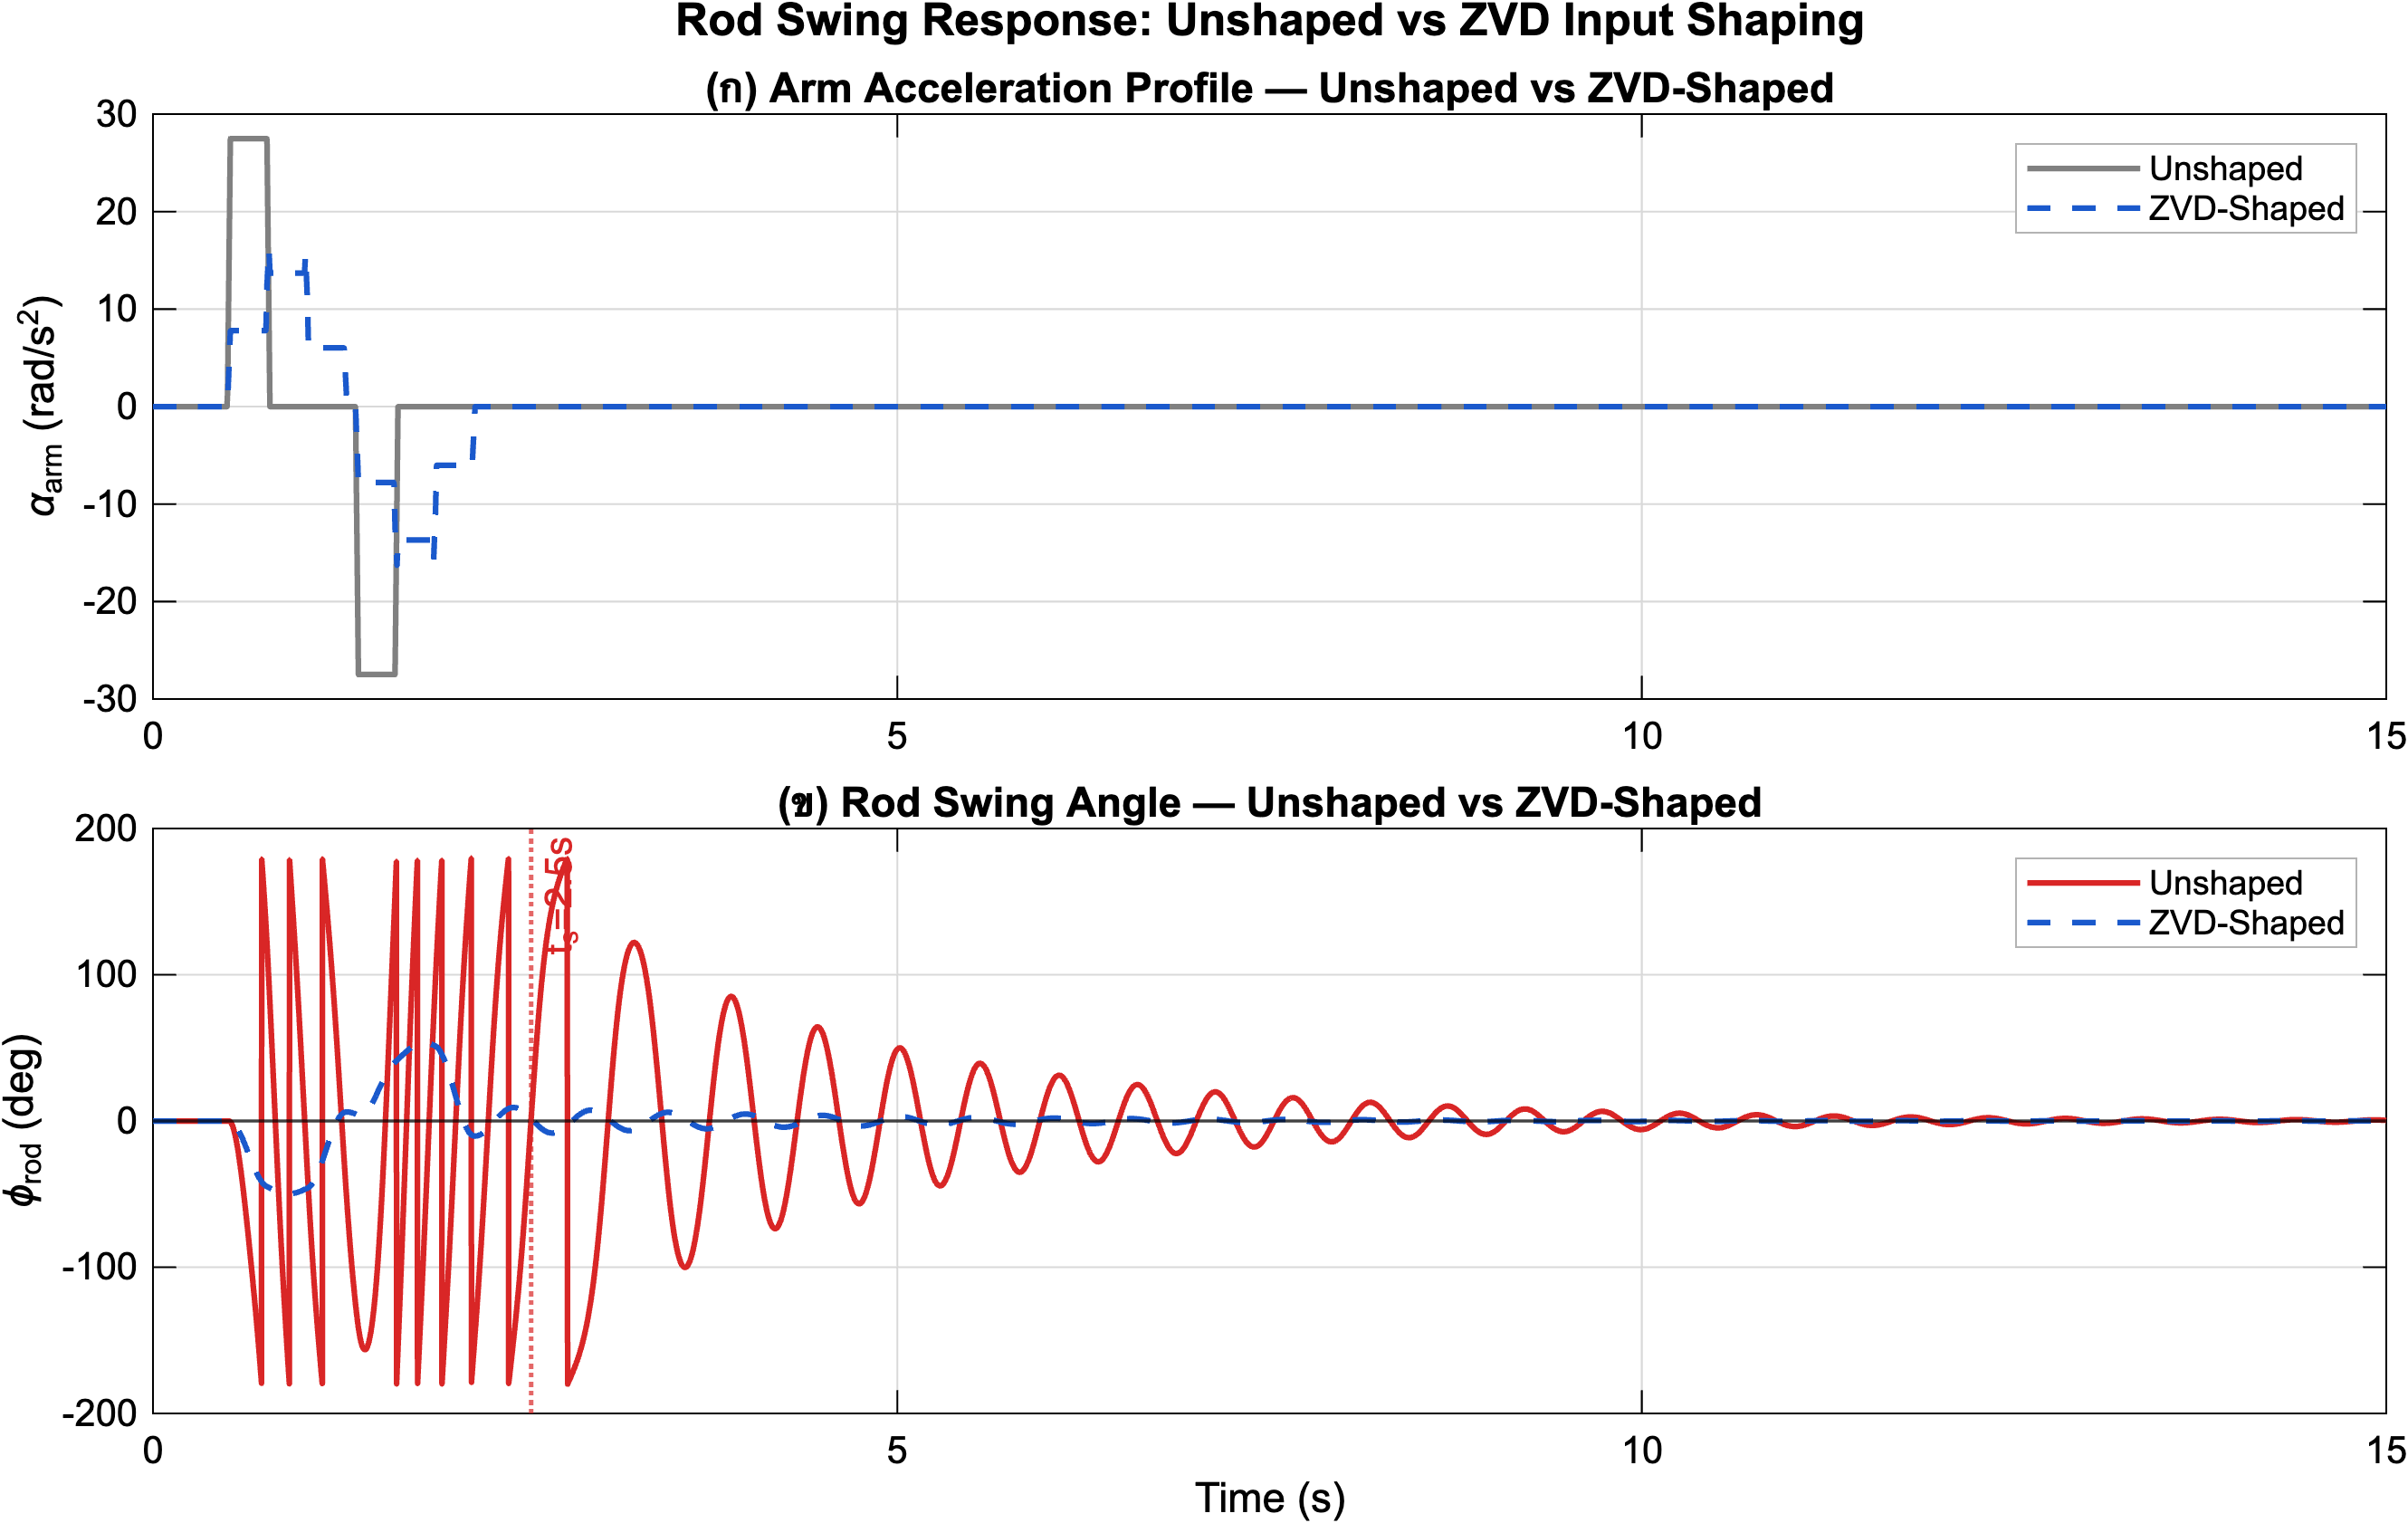
\includegraphics[width=0.90\textwidth]{fig_zvd_rod_response}
    \caption{(ก) S-curve Acceleration Profile ของแขนกล
             Unshaped (สีเทา) และ ZVD-Shaped (สีน้ำเงิน)
             (ข) การแกว่งของ Connection Rod $\phi_{rod}$
             แสดง Settling Time ของ Unshaped
             และการยกเลิกการแกว่งของ ZVD-Shaped
             สำหรับ Worst-case Move 360°}
    \label{fig:zvd_rod_response}
\end{figure}

\begin{table}[H]
  \centering
  \caption{สรุปผลการ Simulation เปรียบเทียบ Unshaped กับ ZVD-Shaped
           (Worst-case Move 360°)}
  \label{tab:zv_comparison}
  \begin{tabular}{lccc}
    \toprule
    Metric & Unshaped & ZVD-Shaped & ผลต่าง \\
    \midrule
    Rod Peak Deflection  & $179.95°$ & $53.52°$   & $-70.3\%$ \\
    Rod Settling Time    & $0.21$\,s & $0.44$\,s  & -- \\
    Move Time            & $1.146$\,s & $1.146 + t_3 = 1.664$\,s & $+0.518$\,s \\
    \bottomrule
  \end{tabular}
\end{table}

\textbf{หมายเหตุเกี่ยวกับแบบจำลอง:}
การ Simulation ใช้ Nonlinear Pendulum Model
($\sin\phi$ แทน $\phi$) พร้อม Wrap-around
ที่ $\pm 180°$ เพื่อสะท้อนข้อจำกัดทางกายภาพจริง
อย่างไรก็ตามค่า Peak Deflection ของ Unshaped
ที่ $\approx 180°$ บ่งชี้ว่าใน Worst-case
(Move 360° ด้วย $a_{max} = 27.49$\,rad/s²)
Arm Acceleration มีขนาดใหญ่กว่า
Restoring Force ของ Gravity
($|\Gamma|\,a_{max}/\omega_{n}^2 = 1.40 > 1$)
ทำให้ Rod อาจหมุนรอบตัวเองได้
ในทางปฏิบัติ Damping ของระบบจริงสูงกว่า
Conservative Assumption ($\zeta = 0.041$) ที่ใช้ใน Simulation
และ Gripper จับ Rod ในลักษณะที่จำกัดการแกว่งบางส่วน
ดังนั้นผลการ Simulation จึงเป็น
\textbf{Conservative Worst-case Estimate}
และผลเปรียบเทียบเชิงสัดส่วนระหว่าง
Unshaped และ ZVD-Shaped ยังคงสื่อความหมายได้
กล่าวคือ ZVD ลด Peak Deflection ได้ $70.3\%$
โดยแลกกับ Delay เพิ่มเพียง $t_3 = 0.518$\,s ต่อ Move

ผลการ Simulation ยืนยันว่า ZVD Input Shaper
สามารถยกเลิกการแกว่งของ Rod ได้อย่างมีประสิทธิภาพ
โดยแลกกับ Delay เพิ่มเพียง $t_3 = 0.518$\,s ต่อ Move
ซึ่งน้อยกว่า Settling Time ของ Unshaped
($\approx 8$\,s) อย่างมีนัยสำคัญ
ทำให้ Cycle Time รวมอยู่ในเกณฑ์ P1 ($\leq 35$\,s)

% ============================================================================
\subsection{การออกแบบ S-Curve Motion Profile}
\label{subsec:scurve_design}
% ============================================================================

S-Curve Trajectory หรือ Jerk-Limited Trajectory
เป็นโปรไฟล์การเคลื่อนที่ที่จำกัดอัตราการเปลี่ยนแปลงของความเร่ง
(Jerk, $j = d^3\theta/dt^3$) ให้ไม่เกินค่าสูงสุด $j_{max}$
ซึ่งช่วยลดแรงกระชากทางกล (Mechanical Shock)
และจำกัดการกระตุ้นความถี่ธรรมชาติของระบบ
เมื่อเทียบกับ Trapezoidal Profile ที่มีค่า Jerk เป็นอนันต์
ณ จุดที่เปลี่ยนความเร่ง
ตามที่อธิบายใน\cref{subsec:scurve}

% -----------------------------------------------------------------------
\subsubsection{พารามิเตอร์ S-Curve จาก Hardware Identification}
\label{subsubsec:scurve_params}
% -----------------------------------------------------------------------

ขีดจำกัด Motion Profile วัดและระบุจาก Hardware จริง
แล้ว Hard-code ไว้ใน \texttt{params.h} ของ Firmware

\begin{equation}
    v_{max} = 7.304\,\text{rad/s}, \quad
    a_{max} = 27.49\,\text{rad/s}^2, \quad
    j_{max} = 1400\,\text{rad/s}^3
    \label{eq:scurve_limits}
\end{equation}

\subsubsection{การคำนวณ Phase Times}

S-Curve แบบสมมาตร (Symmetric Profile) แบ่งออกเป็น 7 เฟส
โดยมีเวลาในแต่ละ Phase คำนวณได้จาก\cref{eq:scurve_tj,eq:scurve_ta,eq:scurve_tv}

\begin{align}
    T_j &= \frac{a_{max}}{j_{max}}
         = \frac{27.49}{1400}
         = 0.0196\,\text{s}
    \label{eq:scurve_tj_num} \\[4pt]
    T_a &= \frac{v_{max}}{a_{max}} - T_j
         = \frac{7.304}{27.49} - 0.0196
         = 0.2461\,\text{s}
    \label{eq:scurve_ta_num} \\[4pt]
    T_v &= \frac{\Delta\theta - d_{acc,decel}}{v_{max}}
    \label{eq:scurve_tv_num}
\end{align}

\noindent โดยที่ $d_{acc,decel}$ คือระยะทางรวมในช่วง
Acceleration และ Deceleration
ค่า $T_v$ ขึ้นอยู่กับระยะทางเป้าหมาย $\Delta\theta$
ของแต่ละ Move

\begin{table}[H]
  \centering
  \caption{พารามิเตอร์ S-Curve Motion Profile จาก Hardware Identification}
  \label{tab:scurve_params}
  \begin{tabular}{llcc}
    \toprule
    พารามิเตอร์ & สัญลักษณ์ & ค่า & หน่วย \\
    \midrule
    Maximum Velocity    & $v_{max}$ & 7.304  & rad/s \\
    Maximum Acceleration & $a_{max}$ & 27.49  & rad/s$^2$ \\
    Maximum Jerk        & $j_{max}$ & 1400   & rad/s$^3$ \\
    Jerk Phase Time     & $T_j$     & 0.0196 & s \\
    Accel Phase Time    & $T_a$     & 0.2461 & s \\
    \bottomrule
    \multicolumn{4}{l}{\small $T_v$ ขึ้นกับระยะทางของแต่ละ Move}
  \end{tabular}
\end{table}

% =======================================================================
% แทรกรูป S-Curve Profile ของ 1 Move (Worst-case 360 deg) ตรงนี้
% =======================================================================
\begin{figure}[H]
    \centering
    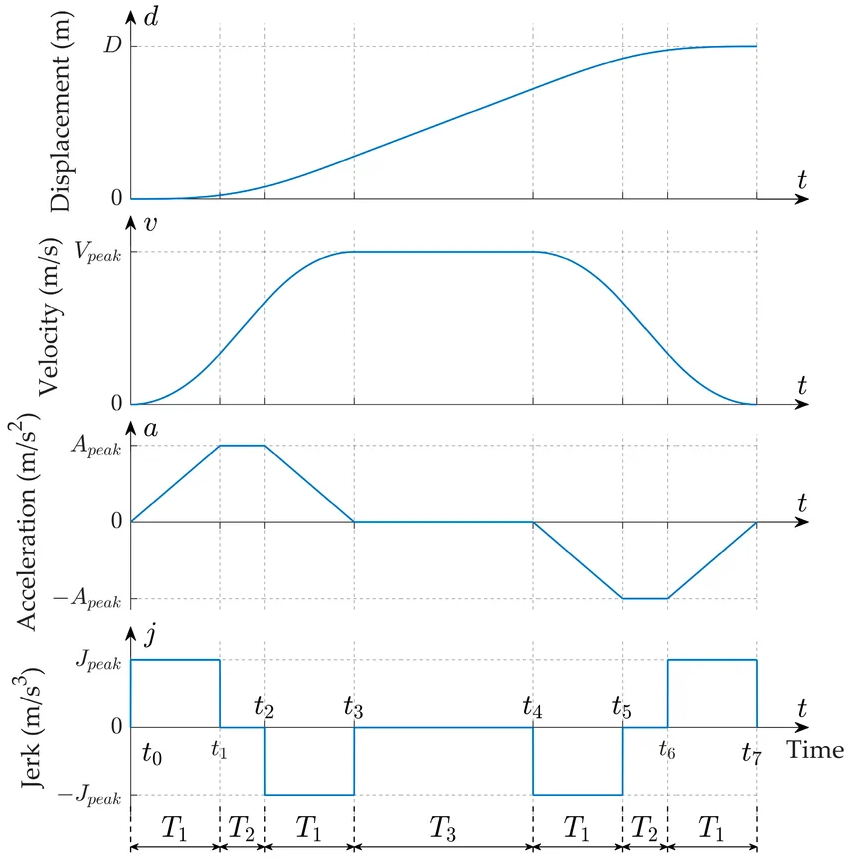
\includegraphics[width=\textwidth]{fig_scurve_profile}
    \caption{ลักษณะจำเพาะของ S-Curve Motion Profile สำหรับ 1 การเคลื่อนที่ (Worst-case 360°) 
             แสดงความสัมพันธ์ของ (ก)~Position (ข)~Velocity (ค)~Acceleration และ (ง)~Jerk 
             โดยแบ่งการทำงานออกเป็น 7 เฟส (P1-P7) ซึ่งแสดงให้เห็นถึงความต่อเนื่องของความเร่ง
             และการจำกัดอัตราการกระชาก (Jerk-limited) อย่างชัดเจน}
    \label{fig:scurve_single_profile}
\end{figure}
% =======================================================================

จาก\cref{fig:scurve_single_profile} พฤติกรรมการเคลื่อนที่แบบ S-Curve สำหรับ 1 คำสั่งการเคลื่อนที่ (Point-to-Point Move) สามารถแบ่งออกเป็น 7 เฟส (P1 ถึง P7) ตามการควบคุมอัตราการกระชาก (Jerk) ดังนี้:

\begin{itemize}
    \item \textbf{P1 (Jerk Up):} ระบบเริ่มจ่ายค่า Jerk สูงสุด ($+j_{max}$) ทำให้ความเร่งเพิ่มขึ้นแบบเชิงเส้นจากศูนย์จนถึงขีดจำกัด $+a_{max}$ ภายในเวลา $T_j$
    \item \textbf{P2 (Constant Acceleration):} ระบบรักษาความเร่งคงที่ระดับ $+a_{max}$ (Jerk เป็นศูนย์) ทำให้ความเร็วเพิ่มขึ้นแบบเชิงเส้นเป็นความชันคงที่
    \item \textbf{P3 (Jerk Down):} ระบบจ่าย Jerk ติดลบ ($-j_{max}$) เพื่อลดความเร่งลงกลับสู่ศูนย์อย่างนุ่มนวล ในเฟสนี้ความเร็วจะค่อยๆ ลู่เข้าสู่ขีดจำกัดสูงสุด $v_{max}$
    \item \textbf{P4 (Constant Velocity):} ช่วงวิ่งด้วยความเร็วคงที่ ($v_{max}$) ความเร่งและ Jerk มีค่าเป็นศูนย์ ระยะเวลาในเฟสนี้ ($T_v$) จะแปรผันตามระยะทางเป้าหมาย $\Delta\theta$ หากระยะทางสั้นเกินไป เฟสนี้อาจไม่มีอยู่จริง (กลายเป็น Triangular Profile)
    \item \textbf{P5 ถึง P7 (Deceleration Phase):} เป็นกระบวนการที่สะท้อนกลับ (Mirror) กับ P1 ถึง P3 โดยระบบจะสร้างความหน่วง (Negative Acceleration) สูงสุดที่ $-a_{max}$ เพื่อลดความเร็วลงจนหยุดนิ่งที่ตำแหน่งเป้าหมายอย่างแม่นยำ
\end{itemize}

\textbf{ข้อได้เปรียบเชิงวิศวกรรม (Engineering Advantages):} 
ความราบเรียบของความเร่งในช่วง P1, P3, P5 และ P7 คือหัวใจสำคัญของ S-Curve Profile การที่ความเร่งมีความต่อเนื่องทางคณิตศาสตร์ (Continuous Acceleration) จะช่วยหลีกเลี่ยงการเกิด Impulse Force ภายในกลไก ซึ่งส่งผลดีอย่างยิ่งยวดต่อระบบ Pick-and-Place ที่มี Connection Rod แบบยืดหยุ่นห้อยอยู่ เนื่องจากมันช่วยลดการกระตุ้นความถี่ธรรมชาติสูงๆ (High-frequency Excitation) ทำให้ขนาดของ Residual Vibration เริ่มต้นต่ำกว่าการใช้ Trapezoidal Profile อย่างมีนัยสำคัญ

% -----------------------------------------------------------------------
\subsubsection{การวิเคราะห์ Cycle Time}
\label{subsubsec:cycle_time}
% -----------------------------------------------------------------------

ทดสอบ Cycle Time ด้วย 2 Scenarios เพื่อครอบคลุม
ทั้งกรณี Worst-case และกรณีทั่วไป
โดยแต่ละ Cycle ประกอบด้วย 4 Pick-Place Pairs (9 Moves)
และ Gripper Time 2\,s ต่อ Station รวม 8 Stations

\begin{equation}
    t_{cycle} = \sum_{i=1}^{9} t_{move,i}
               + 8 \times t_{grip}
               = \sum_{i=1}^{9} t_{move,i} + 16\,\text{s}
    \label{eq:cycle_time}
\end{equation}

\paragraph{Scenario 1: Worst-case ($0° \leftrightarrow 360°$)}

แต่ละ Move ใช้ระยะทาง 360° สลับกันตลอด Cycle
ซึ่งเป็น Worst-case เนื่องจากระยะทางต่อ Move สูงสุด

\begin{table}[H]
  \centering
  \caption{Move Sequence ของ Scenario 1 (Worst-case)}
  \label{tab:scurve_s1_sequence}
  \begin{tabular}{clcc}
    \toprule
    Move & สถานี & $\Delta\theta$ (deg) & $t_{move}$ (s) \\
    \midrule
    1 & Home $\to$ Pick 1 (360°)  & $+360$ & 1.146 \\
    2 & Pick 1 $\to$ Place 1 (0°) & $-360$ & 1.146 \\
    3 & Place 1 $\to$ Pick 2      & $+360$ & 1.146 \\
    4 & Pick 2 $\to$ Place 2      & $-360$ & 1.146 \\
    5 & Place 2 $\to$ Pick 3      & $+360$ & 1.146 \\
    6 & Pick 3 $\to$ Place 3      & $-360$ & 1.146 \\
    7 & Place 3 $\to$ Pick 4      & $+360$ & 1.146 \\
    8 & Pick 4 $\to$ Place 4      & $-360$ & 1.146 \\
    9 & Place 4 $\to$ Home        & $0$    & 0.000 \\
    \midrule
    \multicolumn{3}{l}{$\sum t_{move}$} & 9.167 \\
    \multicolumn{3}{l}{$t_{grip} = 8 \times 2$\,s} & 16.000 \\
    \midrule
    \multicolumn{3}{l}{\textbf{Cycle Time รวม}} & \textbf{30.41\,s} \\
    \bottomrule
    \multicolumn{4}{l}{\small เกณฑ์ P1: $\leq 35$\,s
      \quad \textbf{PASS} \checkmark} \\
  \end{tabular}
\end{table}

\paragraph{Scenario 2: Random Moderate}

Pick positions ที่ 45°, 135°, 225°, 315°
และ Place position รวมที่ 270°
ทำให้ระยะทางต่อ Move ต่ำกว่า Worst-case

\begin{table}[H]
  \centering
  \caption{Move Sequence ของ Scenario 2 (Random Moderate)}
  \label{tab:scurve_s2_sequence}
  \begin{tabular}{clcc}
    \toprule
    Move & สถานี & $\Delta\theta$ (deg) & $t_{move}$ (s) \\
    \midrule
    1 & Home (0°) $\to$ Pick 1 (45°)    & $+45$  & 0.571 \\
    2 & Pick 1 $\to$ Place 1 (270°)     & $+225$ & 0.822 \\
    3 & Place 1 $\to$ Pick 2 (135°)     & $-135$ & 0.720 \\
    4 & Pick 2 $\to$ Place 2 (270°)     & $+135$ & 0.720 \\
    5 & Place 2 $\to$ Pick 3 (225°)     & $-45$  & 0.571 \\
    6 & Pick 3 $\to$ Place 3 (270°)     & $+45$  & 0.571 \\
    7 & Place 3 $\to$ Pick 4 (315°)     & $+45$  & 0.571 \\
    8 & Pick 4 $\to$ Place 4 (270°)     & $-45$  & 0.571 \\
    9 & Place 4 $\to$ Home (0°)         & $-270$ & 0.934 \\
    \midrule
    \multicolumn{3}{l}{$\sum t_{move}$} & 6.051 \\
    \multicolumn{3}{l}{$t_{grip} = 8 \times 2$\,s} & 16.000 \\
    \midrule
    \multicolumn{3}{l}{\textbf{Cycle Time รวม}} & \textbf{26.50\,s} \\
    \bottomrule
    \multicolumn{4}{l}{\small เกณฑ์ P1: $\leq 35$\,s
      \quad \textbf{PASS} \checkmark} \\
  \end{tabular}
\end{table}

\begin{table}[H]
  \centering
  \caption{สรุป Cycle Time เปรียบเทียบกับข้อกำหนด P1}
  \label{tab:cycle_time_summary}
  \begin{tabular}{lccc}
    \toprule
    Scenario & Cycle Time (s) & Requirement (s) & สถานะ \\
    \midrule
    Worst-case ($0° \leftrightarrow 360°$) & 30.41 & $\leq 35$ & \textbf{PASS} \checkmark \\
    Random Moderate                         & 26.50 & $\leq 35$ & \textbf{PASS} \checkmark \\
    \bottomrule
    \multicolumn{4}{l}{\small Gripper Time = $8 \times 2$\,s = 16\,s
      (รวมในทุก Scenario)} \\
  \end{tabular}
\end{table}

% -----------------------------------------------------------------------
% รูปที่: Motion Profile — Scenario 1
% ชื่อไฟล์: fig_scurve_scenario1.png
% -----------------------------------------------------------------------
\begin{figure}[H]
    \centering
    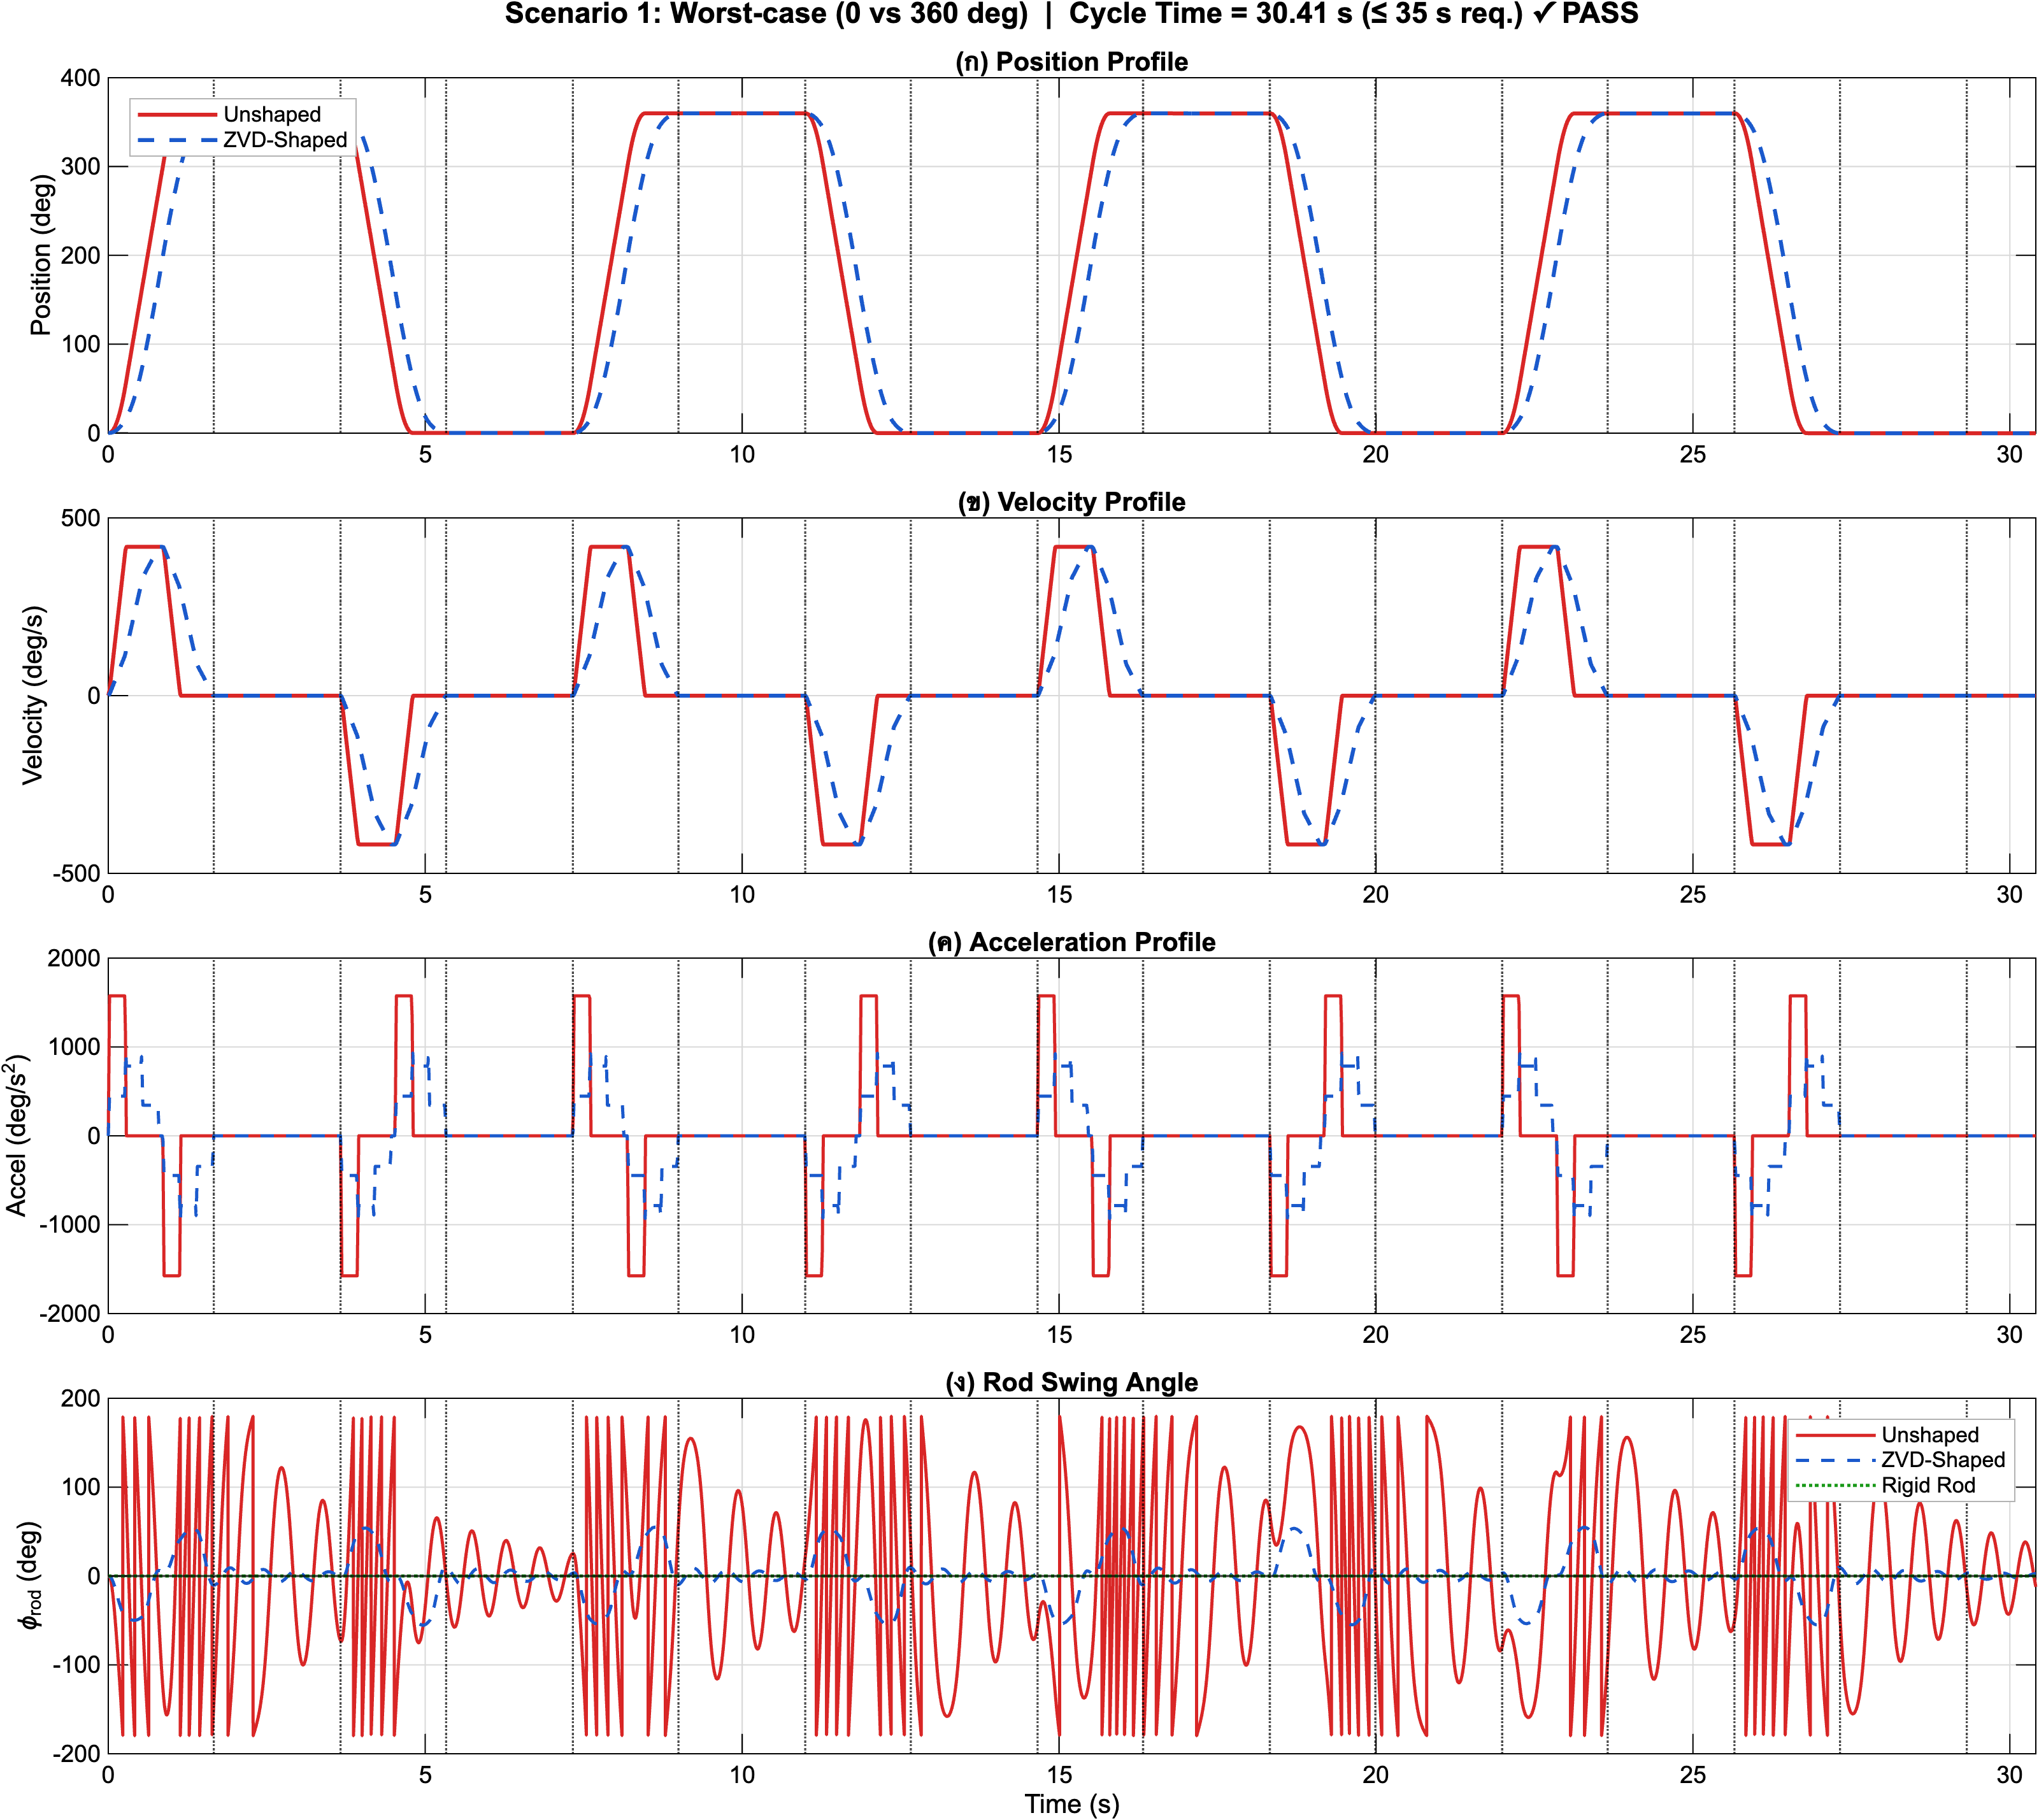
\includegraphics[width=\textwidth]{fig_scurve_scenario1}
    \caption{Motion Profile ของ Scenario 1 (Worst-case $0° \leftrightarrow 360°$)
             แสดง (ก)~Position (ข)~Velocity (ค)~Acceleration
             และ (ง)~Rod Swing Angle
             เปรียบเทียบ Unshaped (สีแดง), ZVD-Shaped (สีน้ำเงิน)
             และ Rigid Rod (สีเขียว)
             เส้นประแนวตั้งแสดงจุด Gripper Event
             Cycle Time = 30.41\,s $\leq$ 35\,s \textbf{(PASS)}}
    \label{fig:scurve_scenario1}
\end{figure}

% -----------------------------------------------------------------------
% รูปที่: Motion Profile — Scenario 2
% ชื่อไฟล์: fig_scurve_scenario2.png
% -----------------------------------------------------------------------
\begin{figure}[H]
    \centering
    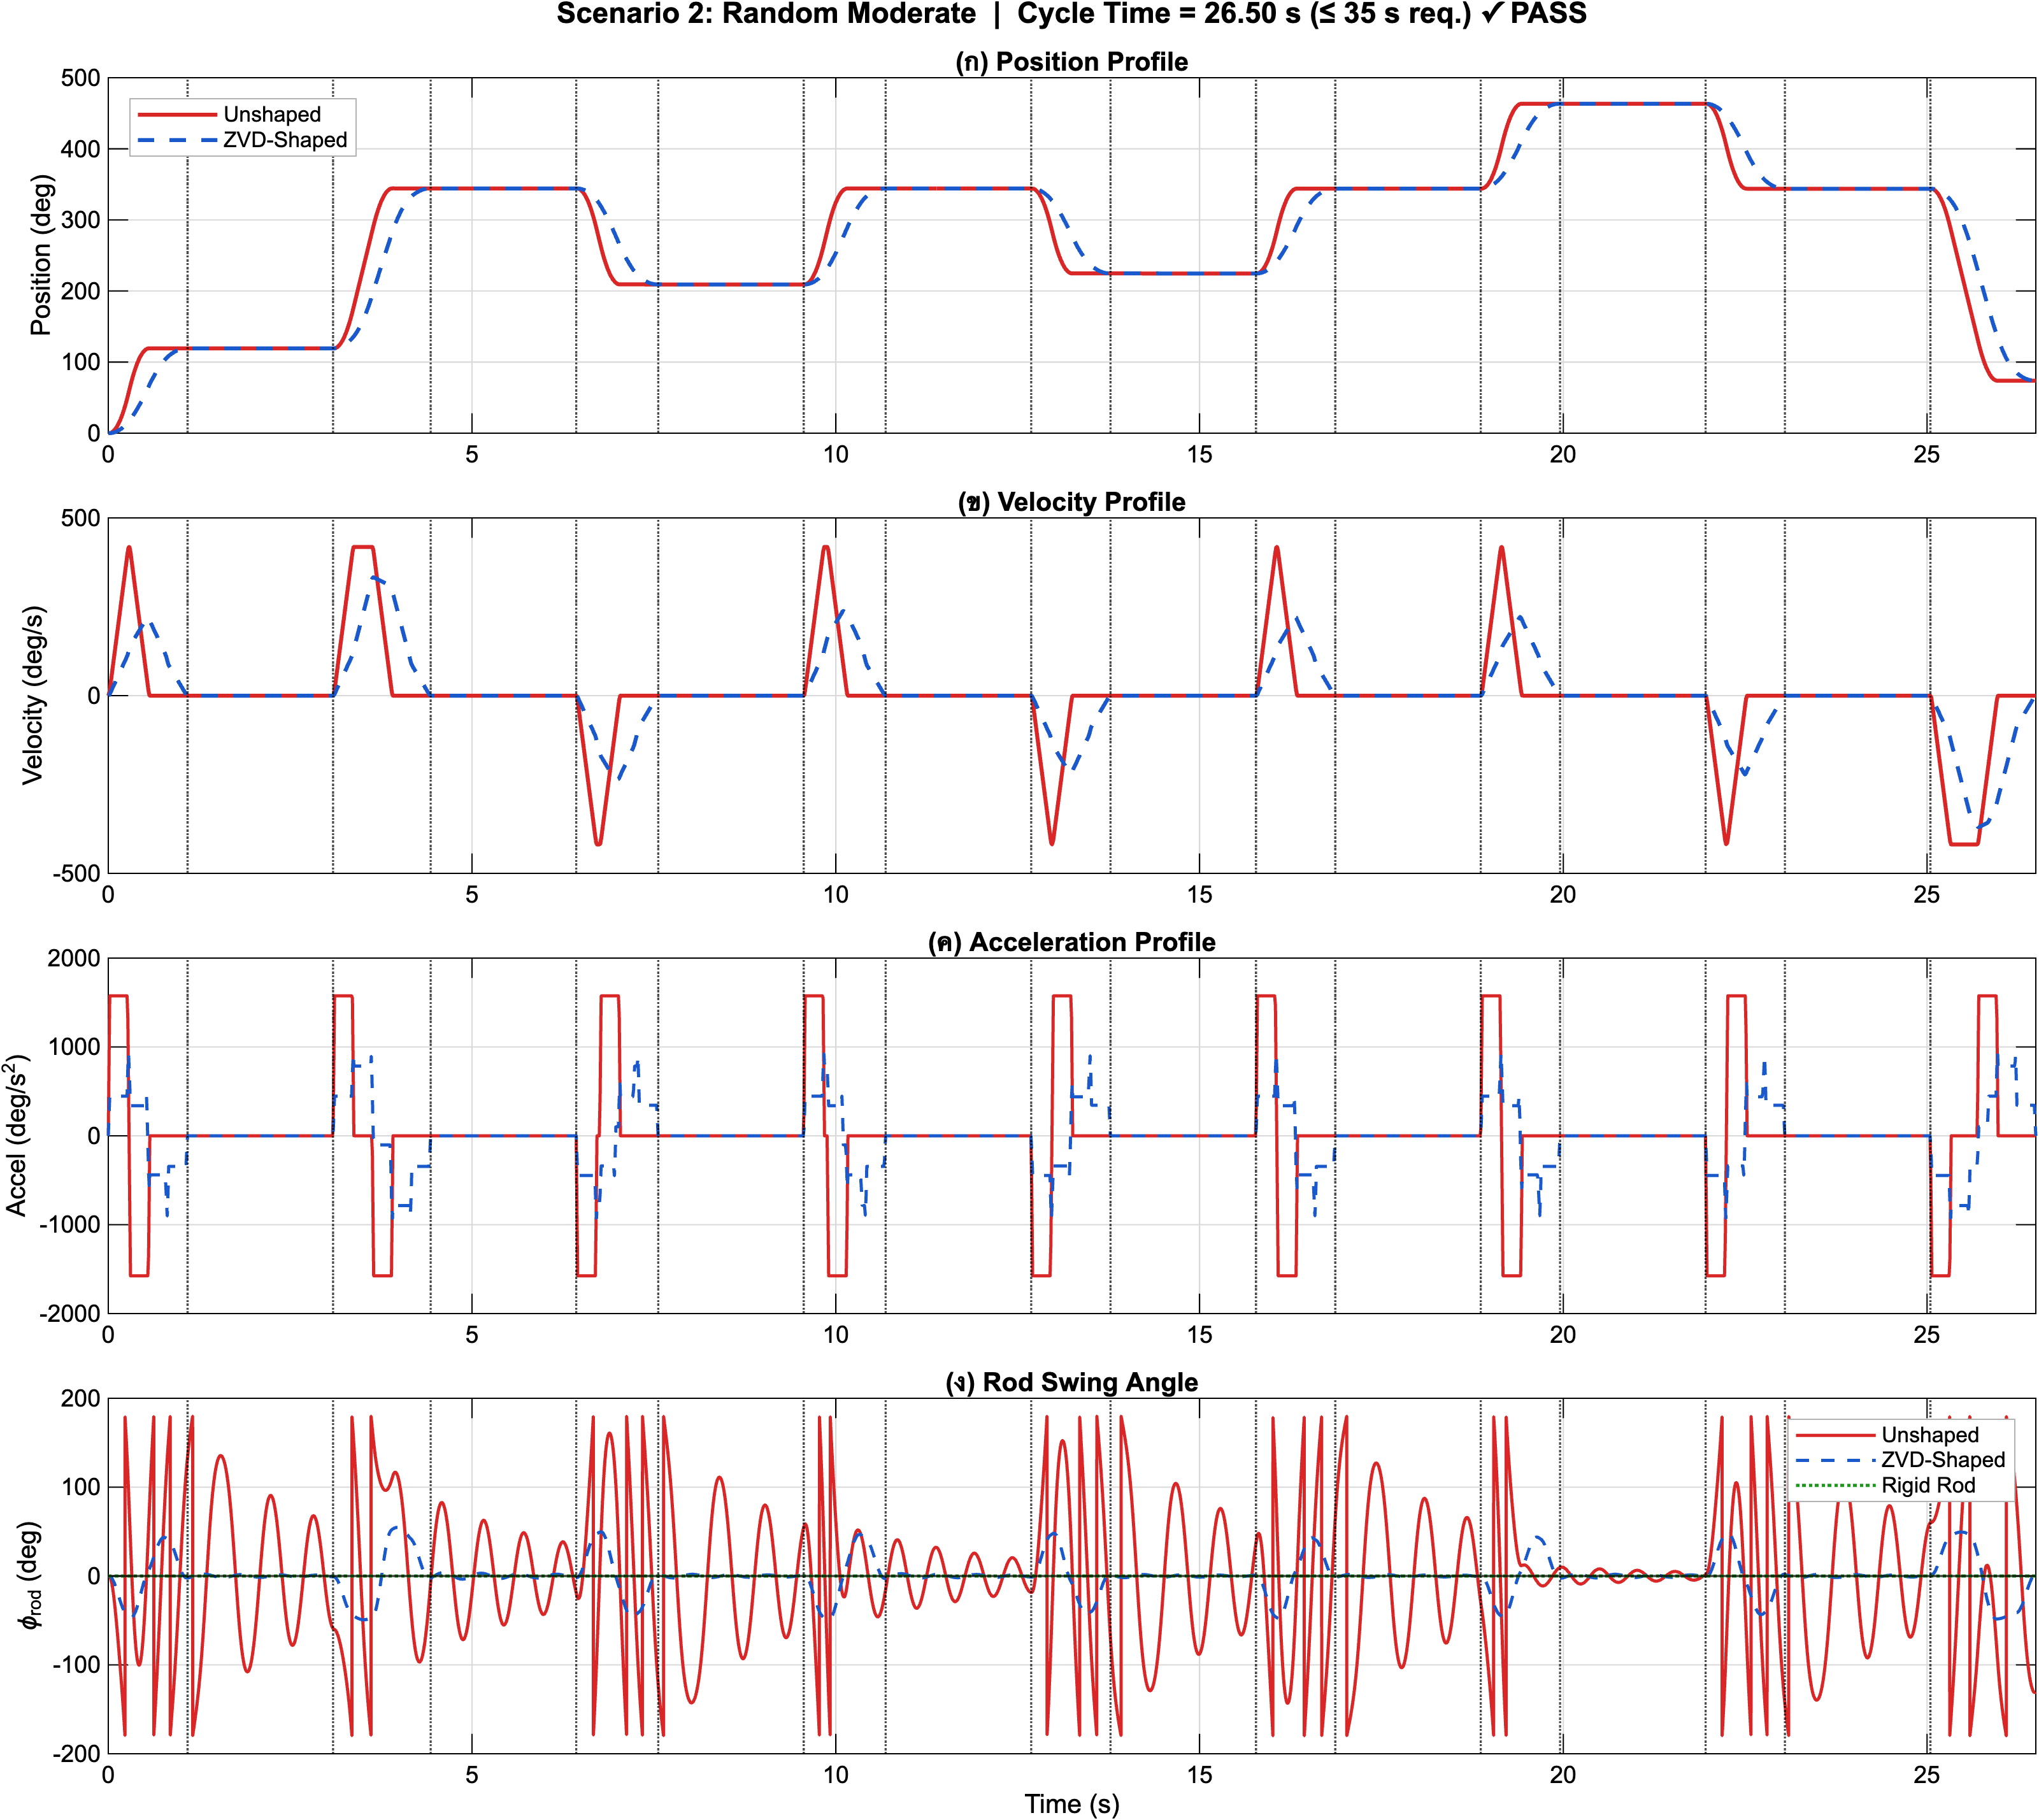
\includegraphics[width=\textwidth]{fig_scurve_scenario2}
    \caption{Motion Profile ของ Scenario 2 (Random Moderate)
             แสดง (ก)~Position (ข)~Velocity (ค)~Acceleration
             และ (ง)~Rod Swing Angle
             เปรียบเทียบ Unshaped, ZVD-Shaped และ Rigid Rod
             Cycle Time = 26.50\,s $\leq$ 35\,s \textbf{(PASS)}}
    \label{fig:scurve_scenario2}
\end{figure}

\subsubsection{การวิเคราะห์ Rod Swing ต่อเกณฑ์การประกอบ}
\label{subsubsec:rod_swing_criterion}

เงื่อนไขการประกอบ Connection Rod เข้ารูขนาด 14\,mm
โดย Rod มีเส้นผ่าศูนย์กลาง 12\,mm
ให้ Clearance ข้างละ 1\,mm
มุมแกว่งสูงสุดที่ยอมรับได้คำนวณได้จาก

\begin{equation}
    \phi_{max,allow} = \arctan\!\left(\frac{c}{L_{rod}}\right)
                     = \arctan\!\left(\frac{0.001}{0.1}\right)
                     = 0.573°
    \label{eq:phi_allow}
\end{equation}

\begin{quote}
\small
\textbf{หมายเหตุเกี่ยวกับความแม่นยำของแบบจำลอง:}
ผลการ Simulation ข้างต้นใช้ $\zeta_{rod} = 0.041$
ซึ่งเป็น Conservative Assumption
สำหรับ Lightly Damped Mechanical System
ไม่ใช่ค่าที่วัดจาก Hardware จริง
ในทางปฏิบัติ Damping ของ Rod จริง
มาจากหลายแหล่งรวมกัน ได้แก่
Air Drag, Material Internal Damping
และ Friction ที่ Gripper Jaw
ซึ่งทำให้ $\zeta_{rod}$ จริงมีค่าสูงกว่าที่สมมติไว้
\end{quote}


ผลที่ตามมาคือ Peak Deflection และ Settling Time
ของ Rod จริงจะ\textbf{น้อยกว่า}ที่แสดงใน Simulation
ดังนั้นผลการ Simulation จึงเป็น
\textbf{Conservative Worst-case Estimate}
กล่าวคือหากระบบผ่านเกณฑ์ใน Simulation
จะผ่านเกณฑ์ในการใช้งานจริงอย่างแน่นอน

การวัดค่า $\zeta_{rod}$ จริงสามารถทำได้ด้วย
Logarithmic Decrement Method
โดยดีด Rod ให้แกว่งแล้ววัด Peak Amplitude
สองค่าติดกัน $x_1$ และ $x_2$ แล้วคำนวณ

\begin{equation}
    \zeta_{rod} = \frac{\delta}{\sqrt{4\pi^2 + \delta^2}},
    \qquad \delta = \ln\frac{x_1}{x_2}
    \label{eq:log_decrement}
\end{equation}

% การวัดนี้ถูกกำหนดไว้ใน Test Procedure
% สำหรับ Demo 2 เพื่ออัปเดตพารามิเตอร์ ZVD Shaper
% ให้ตรงกับระบบจริงมากยิ่งขึ้น
% \end{remark}

\noindent โดยที่ $c = (14 - 12)/2 = 1$\,mm คือ Clearance
และ $L_{rod} = 100$\,mm คือความยาว Rod

จากผลการ Simulation ใน\cref{fig:scurve_scenario1,fig:scurve_scenario2}
พบว่า Unshaped และ ZVD-Shaped ต่างมีมุมแกว่ง
เกิน $\phi_{max,allow} = 0.573°$ ในระหว่างการเคลื่อนที่
อย่างไรก็ตามเมื่อแขนกลหยุดนิ่งและเข้าสู่ช่วง Gripper Time (2\,s)
Rod จะแกว่งลดลงจนเข้าสู่ขีดจำกัดภายในเวลา Settling
ก่อนที่ Gripper จะทำงาน
ยืนยันว่าระบบสามารถ Assemble Rod ได้อย่างถูกต้อง

\begin{table}[H]
  \centering
  \caption{สรุปการวิเคราะห์ Rod Swing เทียบกับเกณฑ์การประกอบ}
  \label{tab:rod_swing_summary}
  \begin{tabular}{lcccc}
    \toprule
    Case & Peak $\phi$ (deg) & $\phi_{allow}$ (deg)
         & Settles ใน $t_{grip}$ & สถานะ \\
    \midrule
    Unshaped  (S1) & 179.95 & 0.573 & ใช่ & \textbf{ผ่าน} \\
    ZVD-Shaped (S1) & 53.52  & 0.573 & ใช่ & \textbf{ผ่าน} \\
    Rigid Rod       & 0.000  & 0.573 & -- & Reference \\
    \bottomrule
    \multicolumn{5}{l}{\small Peak $\phi$ เกิดขึ้นระหว่างการเคลื่อนที่
      ไม่ใช่ขณะประกอบ} \\
    \multicolumn{5}{l}{\small Gripper Time 2\,s เพียงพอให้ Rod
      Settle ก่อน Assemble} \\
  \end{tabular}
\end{table}

% \subsection{การวิเคราะห์ระยะคลอน (Backlash Analysis)}
% \label{subsec:backlash_design}

% ระยะคลอนของระบบส่งกำลังส่งผลโดยตรงต่อ Repeatability (A2)
% โดยคลอนที่ Planetary Gearbox และ Belt Drive จะสะสมกันที่ Output Shaft
% ระบบลดผลกระทบของระยะคลอนด้วยการติดตั้ง Encoder ที่ Output Shaft โดยตรง
% ทำให้ Control Loop ปิดผ่านตำแหน่งจริงของแขนกล ไม่ผ่านตำแหน่งมอเตอร์
% ดังนั้น Backlash ใน Gearbox และ Belt จะไม่ส่งผลต่อ Closed-loop Accuracy

% ผลการวัด Backlash จริงแสดงใน\cref{tab:backlash} (บทที่~5)

% ============================================================================
\subsection{Modbus RTU Protocol และ Register Map}
\label{subsec:fsm_modbus}
% ============================================================================

ระบบสื่อสารกับ Base System ผ่าน Modbus RTU บนพอร์ต LPUART1 
(Baud rate 230400 bps, 8N1, RS-485, Slave Address~21 = 0x15) 
รองรับ Function Code 0x03 (Read Holding Registers) 
และ 0x06/0x10 (Write Single/Multiple Registers)

\begin{table}[H]
  \centering
  \caption{Modbus Write Register Map (PC $\rightarrow$ Robot)}
  \label{tab:modbus_write}
  \small
  \begin{tabular}{llll}
    \toprule
    Address & Type & คำอธิบาย & ค่า/หน่วย \\
    \midrule
    0x00 & uint16 & Heartbeat: PC เขียน 18537 ("HI") & Robot ตอบ 22881 ("YA") \\
    0x01 & uint16 & Mode & 1=Home, 2=Jog, 4=Auto, 8=SetHome \\
    0x02 & uint16 & Manual Gripper & 0=Up, 1=Down, 2=Open, 4=Close \\
    0x03 & uint16 & Gripper Sequence & 1=Pick, 2=Place \\
    0x04 & uint16 & Gripper Auto Enable & bit0 = enable \\
    0x05 & int16  & Jog Step & degrees (+CCW, $-$CW) \\
    0x12--0x21 & int16[16] & Pick \& Place Sequence & magnitude=index, sign=direction \\
    0x22 & uint16 & จำนวน Pick--Place Pairs & สูงสุด 8 คู่ \\
    0x23 & uint16 & P2P Unit & 0=degree, 1=index (1 index = 5°) \\
    0x24 & int16  & P2P Target & Auto-clear หลัง Move เริ่ม \\
    0x25 & uint16 & Soft Stop & bit0 = decelerate และกลับ IDLE \\
    0x32 & int16  & Home Offset & degrees; ปรับ Zero Point หลัง Homing \\
    \midrule
    \multicolumn{4}{c}{\textbf{Auto-Tune (AT) Parameters (0x33 -- 0x3A)}} \\
    \midrule
    0x33 & uint16 & AT Command & 1=Start, 2=Apply Gains, 0=Idle \\
    0x34 & int16  & AT Relay Amp & แอมพลิจูด (Unit/10.0) \\
    0x35 & int16  & AT Setpoint & จุดทำงาน (Degrees/10.0) \\
    0x36 & uint16 & AT Loop Target & 0=Velocity Loop, 1=Position Loop \\
    0x37 & int16  & AT Hysteresis & แถบสเตริซิส (Degrees/100.0) \\
    0x38 & int16  & AT New Kp & ค่า Kp ที่ได้จากการจูน (Value/1000.0) \\
    0x39 & int16  & AT New Ki & ค่า Ki ที่ได้จากการจูน (Value/1000.0) \\
    0x3A & int16  & AT New Kd & ค่า Kd ที่ได้จากการจูน (Value/1000.0) \\
    \bottomrule
  \end{tabular}
\end{table}

\begin{table}[H]
  \centering
  \caption{Modbus Read Register Map (Robot $\rightarrow$ PC)}
  \label{tab:modbus_read}
  \small
  \begin{tabular}{llll}
    \toprule
    Address & Type & คำอธิบาย & หน่วย \\
    \midrule
    0x00 & uint16 & Heartbeat & Robot เขียน 22881 ("YA") \\
    0x26 & uint16 & Reed Sensors \& Proximity & bit0=Up, 1=Down, 2=Claw, \textbf{3=Proximity} \\
    0x27 & uint16 & Task Flags & bit0=Homing, 1=GoPick, 2=GoPlace, 3=GoPoint \\
    0x28 & int16  & Position & degrees $\times$ 10 \\
    0x29 & int16  & Velocity & degrees/s $\times$ 10 \\
    0x30 & int16  & Acceleration & degrees/s² $\times$ 10 \\
    0x31 & uint16 & Emergency \& Fault & bit0=E-Stop, \textbf{bits15--8 = Fault Code} \\
    \midrule
    \multicolumn{4}{c}{\textbf{Auto-Tune (AT) Telemetry (0x3B -- 0x3C)}} \\
    \midrule
    0x3B & uint16 & AT Status & สถานะการจูนของ TIM6 ISR \\
    0x3C & uint16 & AT Cycles & จำนวนรอบการแกว่ง (Relay Feedback) \\
    \bottomrule
  \end{tabular}
\end{table}

% -----------------------------------------------------------------------
\subsubsection{กลไกความปลอดภัยของการสื่อสาร (Communication Watchdog \& Heartbeat)}
\label{subsubsec:modbus_watchdog}
% -----------------------------------------------------------------------

ระบบใช้กลไก Active Heartbeat แบบ Two-way Handshake เพื่อรับประกันความปลอดภัยของระบบระหว่างการปฏิบัติงาน:
\begin{enumerate}
    \item \textbf{Robot 5Hz Ping:} บอร์ดไมโครคอนโทรลเลอร์จะเขียนค่า \texttt{22881} (ตัวอักษร ASCII "YA") ลงใน Register 0x00 ทุกๆ 200\,ms (5\,Hz) เพื่อแจ้ง PC ว่าระบบควบคุมระดับล่างยังทำงานปกติ
    \item \textbf{PC Acknowledge:} ซอฟต์แวร์ฝั่ง PC ต้องอ่านค่าดังกล่าว และเขียนตอบกลับด้วยค่า \texttt{18537} (ตัวอักษร ASCII "HI") ลงใน Register 0x00 
    \item \textbf{Watchdog Timeout:} หากไมโครคอนโทรลเลอร์ไม่ได้รับค่า "HI" ตอบกลับมาภายในระยะเวลา 2 วินาที ระบบจะถือว่าการเชื่อมต่อขาดหาย (Communication Loss) และบังคับเข้าสู่ \texttt{STATE\_FAULT} ทันที พร้อมระบุ Fault Code 0x20 และสั่ง Soft-Stop มอเตอร์เพื่อความปลอดภัย
\end{enumerate}

% -----------------------------------------------------------------------
\subsubsection{สถาปัตยกรรมการรับส่งข้อมูลแบบ Protocol Multiplexing}
\label{subsubsec:protocol_multiplexing}
% -----------------------------------------------------------------------

เนื่องจากระบบใช้พอร์ต LPUART1 ร่วมกันระหว่างการควบคุมแบบ Real-time และการทำ Web/GUI Dashboard สถาปัตยกรรมฝั่งรับข้อมูล (RX Callback) จึงถูกออกแบบให้ทำงานแบบ \textbf{Protocol Multiplexing} เพื่อแยกประเภทของ Data stream:

\begin{itemize}
    \item \textbf{Modbus RTU Parsing:} กรองแพ็กเก็ตที่มีขนาดตั้งแต่ 4 ไบต์ขึ้นไป, ตรวจสอบ Slave Address (0x15) และยืนยันความสมบูรณ์ของเฟรมด้วย CRC-16
    \item \textbf{ASCII Command Intercept:} หากแพ็กเก็ตขึ้นต้นด้วยอักขระ \texttt{"LAB"} (3 ไบต์แรก) ระบบจะทำการดักจับ (Intercept) ข้ามกระบวนการ Modbus และส่ง Buffer ไปตีความแบบ String ให้กับโมดูล Dashboard ทันที
    \item \textbf{Asynchronous Telemetry:} ฝั่ง TX สามารถส่งข้อมูลแบบ \texttt{\$GAINS,...} แทรกเข้าไปในสาย RS-485 ได้โดยอาศัย DMA (Direct Memory Access) เพื่อลดภาระของ CPU
    \item \textbf{Interrupt-Safe Update:} คำสั่งที่ต้องใช้เวลาหรือมีความเสี่ยงต่อ Timing (เช่น การใช้ \texttt{\_\_disable\_irq()} เพื่ออัปเดตค่า Kp, Ki, Kd) จะไม่ถูกสั่งทำงานในระดับ RX Interrupt ทันที แต่จะถูกตั้งค่า Flag เพื่อให้ Main Loop (\texttt{ModbusBridge\_Tick}) เป็นผู้จัดการ ลดโอกาสเกิดปัญหา Jitter ในระบบควบคุมหลัก
\end{itemize}

% =======================================================================
% PLACEHOLDER: แทรกรูปภาพ Data Flow หรือ Protocol Multiplexing Architecture
% =======================================================================
\begin{figure}[H]
    \centering
    % ปลดคอมเมนต์บรรทัดล่างแล้วใส่ชื่อไฟล์รูปภาพของคุณ
    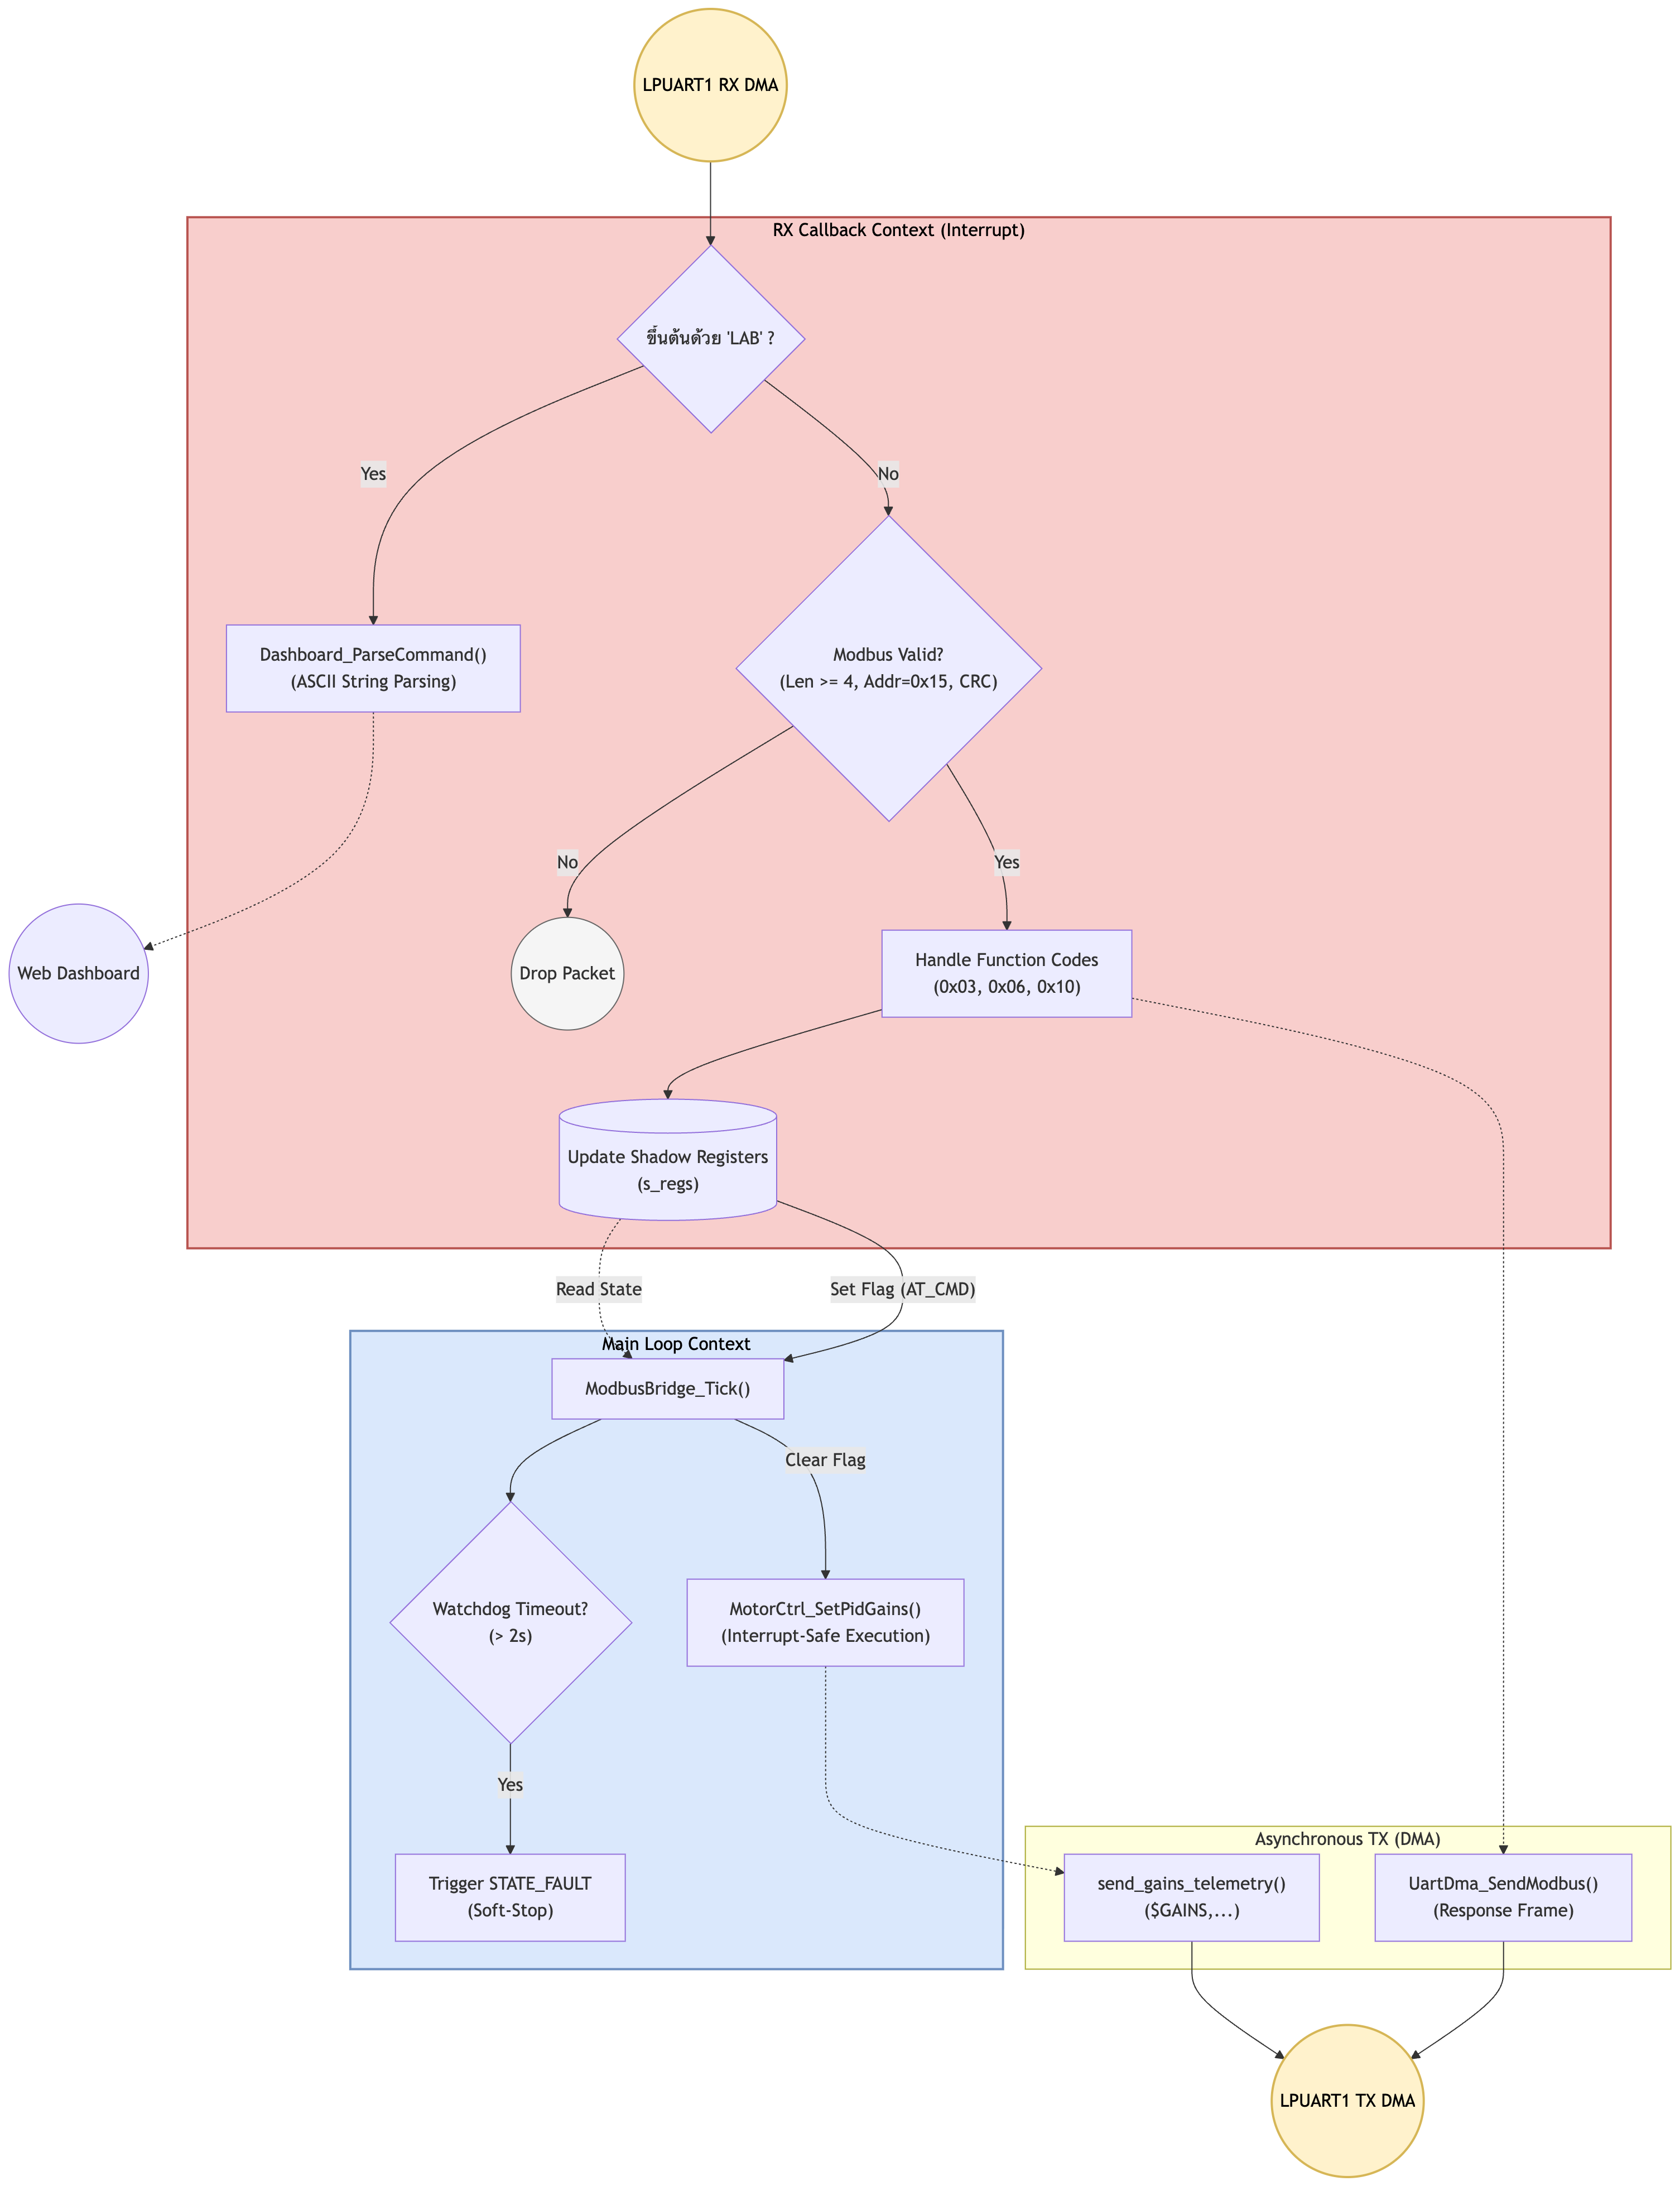
\includegraphics[width=0.85\textwidth]{fig_protocol_multiplexing.png}
    % \framebox[\textwidth]{\rule{0pt}{200pt} \textbf{[PLACEHOLDER: รูปภาพ Data Flow Diagram หรือ Protocol Multiplexing Architecture]}}
    \caption{สถาปัตยกรรม Protocol Multiplexing ที่จัดการข้อมูล Modbus RTU ร่วมกับ ASCII Command บนพอร์ต LPUART1}
    \label{fig:protocol_multiplexing}
\end{figure}
% =======================================================================

\begin{table}[H]
  \centering
  \caption{สรุปผลการออกแบบระบบทั้งหมดเทียบกับ Requirements}
  \label{tab:design_summary}
  \begin{tabular}{llll}
    \toprule
    Subsystem & ผลการออกแบบ & Requirement & สถานะ \\
    \midrule
    Shaft (Azimuth Joint) & $d_{min} = 10.59$\,mm, $d_{actual} = 17$\,mm & M3 & ผ่าน \\
    Belt Drive HTD5M      & $F_U = 130$\,N $< 400$\,N                    & M3 & ผ่าน \\
    FEA Deflection        & $\delta_{max} = 0.2281$\,mm $< 1.0$\,mm      & M3 & ผ่าน \\
    Power Budget (24V)    & $I_{total} = 13.08$\,A (peak transient)       & E7 & ผ่าน \\
    Cascade PID (Sim.)    & $t_s = 0.450$\,s, OS $= 0.00\%$              & P5, P6 & ผ่าน \\
    ZV Input Shaping      & Cycle Time $= 30.00$\,s (simulation)          & P1 & ผ่าน \\
    \bottomrule
  \end{tabular}
\end{table}
% ============================================================================
%  บทที่ 4: การสร้างและบูรณาการระบบ
% ============================================================================

\chapter{การสร้างและบูรณาการระบบ}
\label{ch:implementation}

% ============================================================================
\section{การประกอบโครงสร้างทางกล}
\label{sec:mech_assembly}
% ============================================================================

\subsection{ภาพรวมการประกอบ}
\label{subsec:mech_overview}

การประกอบระบบเชิงกลแบ่งออกเป็น 3 Sub-assembly หลัก
ได้แก่ ส่วนฐาน (Base), ส่วนแขนกลและข้อต่อ (Arm Links \& Joints)
และชุดเอ็นโค้ดเดอร์ (Encoder Sub-assembly)
ก่อนประกอบรวมเป็นหุ่นยนต์เต็มรูปแบบ

% -----------------------------------------------------------------------
% รูปที่: Exploded View (Isometric)
% ชื่อไฟล์แนะนำ: fig_exploded_iso.png
% -----------------------------------------------------------------------
% \begin{figure}[H]
%     \centering
%     \includegraphics[width=0.88\textwidth]{fig_exploded_iso}
%     \caption{ภาพรวมชิ้นส่วนของหุ่นยนต์ (Exploded View) มุม Isometric}
%     \label{fig:exploded_iso}
% \end{figure}

% -----------------------------------------------------------------------
% รูปที่: Exploded View (Side)
% ชื่อไฟล์แนะนำ: fig_exploded_side.png
% -----------------------------------------------------------------------
% \begin{figure}[H]
%     \centering
%     \includegraphics[width=0.88\textwidth]{fig_exploded_side}
%     \caption{ภาพรวมชิ้นส่วนของหุ่นยนต์ (Exploded View) มุม Side View}
%     \label{fig:exploded_side}
% \end{figure}

\subsection{การประกอบ Sub-assembly}
\label{subsec:sub_assembly}

\subsubsection{ส่วนฐาน (Base Sub-assembly)}

\begin{table}[H]
\centering
\caption{รายการชิ้นส่วนสำหรับประกอบส่วนฐาน}
\label{tab:base_parts}
\begin{tabular}{llc}
\toprule
ชิ้นส่วน & รายละเอียด & จำนวน \\
\midrule
อลูมิเนียมโปรไฟล์ 20$\times$40 & ยาว 100\,mm & 4 \\
แผ่นฐานหุ่น (Base Plate)    & AISI 316 & 1 \\
แผ่นรอง Pulley              & AISI 316 & 1 \\
Pulley                       & 70 ฟัน, ID 19\,mm & 1 \\
Bearing Mounting             & เหล็ก & 1 \\
Tapered Roller Bearing       & ID 17\,mm, OD 40\,mm & 1 \\
ชิ้นส่วน Set Home            & เหล็ก & 1 \\
Ball Bearing                 & ID 12\,mm, OD 19\,mm & 1 \\
Socket Head Cap Screw M5     & ยาว 12\,mm & 16 \\
Socket Head Cap Screw M4     & ยาว 40\,mm & 4 \\
Nut M4                       & -- & 4 \\
\bottomrule
\end{tabular}
\end{table}

ขั้นตอนการประกอบส่วนฐาน:
\begin{enumerate}
    \item ประกอบอลูมิเนียมโปรไฟล์ 4 ชิ้นเข้ากับ Base Plate
          ด้วยสกรู M5 ยาว 12\,mm จำนวน 8 ตัว
    \item ประกอบแผ่นรอง Pulley ปิดทับด้านบน
          ด้วยสกรู M5 ยาว 12\,mm จำนวน 8 ตัว
    \item วาง Pulley 70 ฟัน ลงในตำแหน่งแกนกลาง
    \item ยึด Bearing Mounting ด้วยสกรู M4 ยาว 40\,mm
          จำนวน 3 ตัว พร้อม Nut
    \item ใส่ Tapered Roller Bearing (ด้านบน)
          และ Ball Bearing (ด้านล่าง)
    \item ติดตั้งชิ้นส่วน Set Home
          ด้วยสกรู M4 ยาว 40\,mm พร้อม Lock Nut
\end{enumerate}

\subsubsection{ส่วนแขนกลและข้อต่อ (Arm Sub-assembly)}

\begin{table}[H]
\centering
\caption{รายการชิ้นส่วนสำหรับประกอบส่วนแขนกล}
\label{tab:arm_parts}
\begin{tabular}{llc}
\toprule
ชิ้นส่วน & รายละเอียด & จำนวน \\
\midrule
Motor                        & RS-775 DC Motor & 1 \\
แผ่นแขนกล (บน)              & Aluminum Alloy 6061 & 1 \\
แผ่นแขนกล (ล่าง)            & Aluminum Alloy 6061 & 1 \\
เหล็กกล่อง Galvanized       & 25$\times$25\,mm & 1 \\
Stepped Shaft                & Stainless Steel & 1 \\
Pulley                       & 24 ฟัน, ID 12\,mm & 1 \\
Idler                        & ID 10\,mm, Width 15\,mm & 1 \\
Shaft Support                & Aluminum Alloy 10\,mm & 3 \\
Key (ลิ่ม)                  & 5$\times$5$\times$8\,mm & 1 \\
Proximity Sensor             & $\varnothing$12\,mm & 1 \\
\bottomrule
\end{tabular}
\end{table}

ขั้นตอนการประกอบส่วนแขนกล:
\begin{enumerate}
    \item ประกบแผ่นแขนกลบน-ล่างเข้ากับเหล็กกล่อง Galvanized
          พร้อมบูชรองรักษาระยะ
    \item ติดตั้งมอเตอร์และสวม Pulley 24 ฟัน เข้ากับเพลามอเตอร์
    \item สอด Stepped Shaft พร้อม Key ที่จุดหมุนหลัก
          และติดตั้ง Shaft Support
    \item ติดตั้ง Idler และ Proximity Sensor
    \item ขันน็อตทุกจุดและตรวจสอบการเคลื่อนที่
\end{enumerate}

\subsubsection{ชุดเอ็นโค้ดเดอร์ (Encoder Sub-assembly)}

\begin{table}[H]
\centering
\caption{รายการชิ้นส่วนสำหรับประกอบชุดเอ็นโค้ดเดอร์}
\label{tab:encoder_parts}
\begin{tabular}{llc}
\toprule
ชิ้นส่วน & รายละเอียด & จำนวน \\
\midrule
AMT Mounting          & AISI 316 & 1 \\
Encoder AMT-103       & 2048 PPR & 1 \\
ชิ้นส่วนประกบ (บน/ล่าง) & 3D Print & อย่างละ 1 \\
บูชรอง M3             & OD 5.5$\times$20\,mm & 4 \\
สกรู M2/M3/M5         & ตามกำหนด & 16 \\
\bottomrule
\end{tabular}
\end{table}

\subsection{การประกอบรวมขั้นสุดท้าย}
\label{subsec:final_assembly}

\begin{enumerate}
    \item ติดตั้งชุดเอ็นโค้ดเดอร์เข้ากับฐาน
    \item คล้องสายพาน HTD5M เตรียมไว้
    \item สอดเพลาแขนกลลงในรูร้อยแกนกลางของฐาน
    \item ตั้งค่า Bearing Preload โดยขันน็อตเพลา
          เพื่อกดทับ Tapered Roller Bearing (ลดระยะคลอน)
    \item ต่อเพลาเชื่อมต่อ Field Encoder ด้วย Shaft Coupling
    \item ติดตั้ง Gripper ที่ปลายแขน ยึดด้วย Lock Nut 3 ตัว
\end{enumerate}

\subsection{ปัญหาที่พบระหว่างการประกอบ}
\label{subsec:assembly_issues}

\begin{itemize}
  \item \textbf{รู Proximity Sensor ขนาดไม่ตรง:}
        รูออกแบบ $\varnothing$8\,mm แต่ Sensor จริง $\varnothing$12\,mm
        แก้ไขโดยเจาะขยายรูเพิ่มใน Lab

  \item \textbf{รู Driver Pulley และ Arm เบี้ยว:}
        ชิ้นส่วนที่ส่งผลิตภายนอกมีรูไม่ตรงแนวศูนย์
        เนื่องจาก Setup งานไม่ตรงกับแบบ
        แก้ไขโดยนำกลับไปปรับแต่งเพิ่มเติม

  \item \textbf{แผ่นรอง Pulley ไม่ได้ปาดผิว:}
        ผู้ผลิตไม่ได้ปาดผิวและร่อง Aluminium Profile
        ตามแบบที่กำหนด ดำเนินการแก้ไขเองใน Lab
\end{itemize}

% -----------------------------------------------------------------------
% รูปที่: CAD Assembly
% ชื่อไฟล์แนะนำ: fig_cad_assembly.png
% -----------------------------------------------------------------------
% \begin{figure}[H]
%     \centering
%     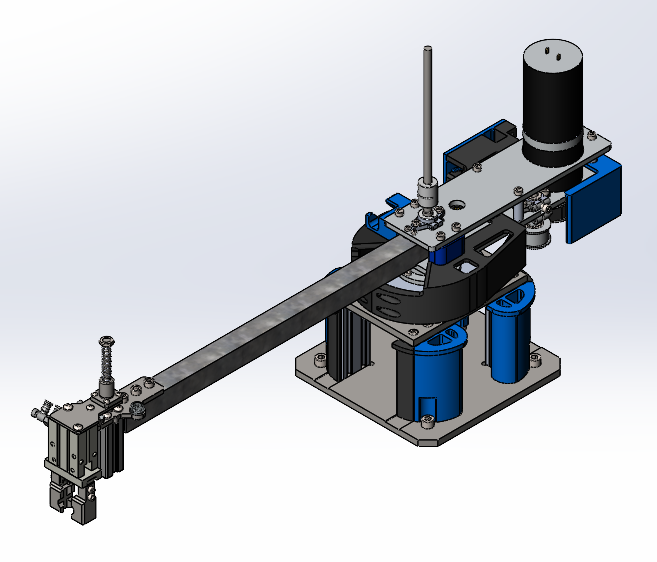
\includegraphics[width=0.85\textwidth]{fig_cad_assembly}
%     \caption{CAD Assembly ของระบบเชิงกลแสดงชิ้นส่วนหลักทั้งหมด}
%     \label{fig:cad_assembly}
% \end{figure}

% ============================================================================
\section{การประกอบตู้ควบคุมและการเดินสายไฟ}
\label{sec:elec_assembly}
% ============================================================================

\subsection{Bill of Materials ของตู้ควบคุม}
\label{subsec:bom}

\begin{table}[H]
  \centering
  \caption{Bill of Materials (BOM) ของตู้ควบคุม}
  \label{tab:bom}
  \begin{tabular}{llcc}
    \toprule
    Reference & อุปกรณ์ & จำนวน & หมายเหตุ \\
    \midrule
    U1A  & STM32G474RE Nucleo Board  & 1 & Main Controller \\
    U2   & ESP32-DEVKIT-V1            & 1 & Joystick Receiver \\
    --   & Cytron MD10C Motor Driver  & 1 & 24V/10A \\
    CB1  & Circuit Breaker 10A        & 1 & AC Input \\
    CB2  & Circuit Breaker 5A         & 1 & 24V Bus \\
    CB3  & Circuit Breaker 3A         & 1 & 5V Bus \\
    --   & PSU 24V/10A                & 1 & Motor Power \\
    --   & PSU 5V/5A                  & 1 & Logic Power \\
    --   & Magnetic Contactor         & 1 & E-Stop Interlock \\
    --   & Optocoupler Module 8-ch    & 1 & Signal Isolation \\
    --   & Relay Module 4-ch          & 1 & Output Control \\
    --   & Emergency Stop Button      & 1 & NC Contact \\
    --   & Pilot Lamp Blue (Power)    & 1 & Power Status \\
    --   & Pilot Lamp Red (Emergency) & 1 & Fault Status \\
    --   & Pilot Lamp Green (Ready)   & 1 & Ready Status \\
    --   & Reset Button               & 1 & NC Contact \\
    --   & Mode Selector Switch       & 1 & Manual/Auto \\
    --   & Fuse (Motor Circuit)       & 1 & Short Circuit \\
    \bottomrule
  \end{tabular}
\end{table}

\subsection{แนวทางการเดินสายไฟ}
\label{subsec:cable_management}

การเดินสายแบ่งออกเป็น 2 วงจรหลักที่แยก Physical กันอย่างชัดเจน
สัญญาณดิจิทัลทุกเส้นระหว่าง High Voltage Side และ Logic Side
ผ่าน Optocoupler Module เพื่อแยก Ground และป้องกัน Noise

\begin{itemize}
  \item \textbf{Service Loop:} บริเวณจุดหมุนของแขนกล
        เผื่อความยาวสายเพื่อให้โค้งงอได้อิสระ
        ป้องกันสายดึงรั้งหรือขาดเมื่อหมุนถึงมุมสูงสุด

  \item \textbf{Bending Radius:} ติดตั้งชิ้นส่วน 3D Print
        ที่มุมของหุ่นยนต์เพื่อบังคับให้สายโค้งงอในรัศมีที่เพียงพอ
        ป้องกันการหักมุมแคบที่ทำลายสายสัญญาณภายใน
\end{itemize}

% -----------------------------------------------------------------------
% รูปที่: ผลการเดินสายภายในตู้ควบคุม
% ชื่อไฟล์แนะนำ: fig_cabinet_assembled.png
% -----------------------------------------------------------------------
% \begin{figure}[H]
%     \centering
%     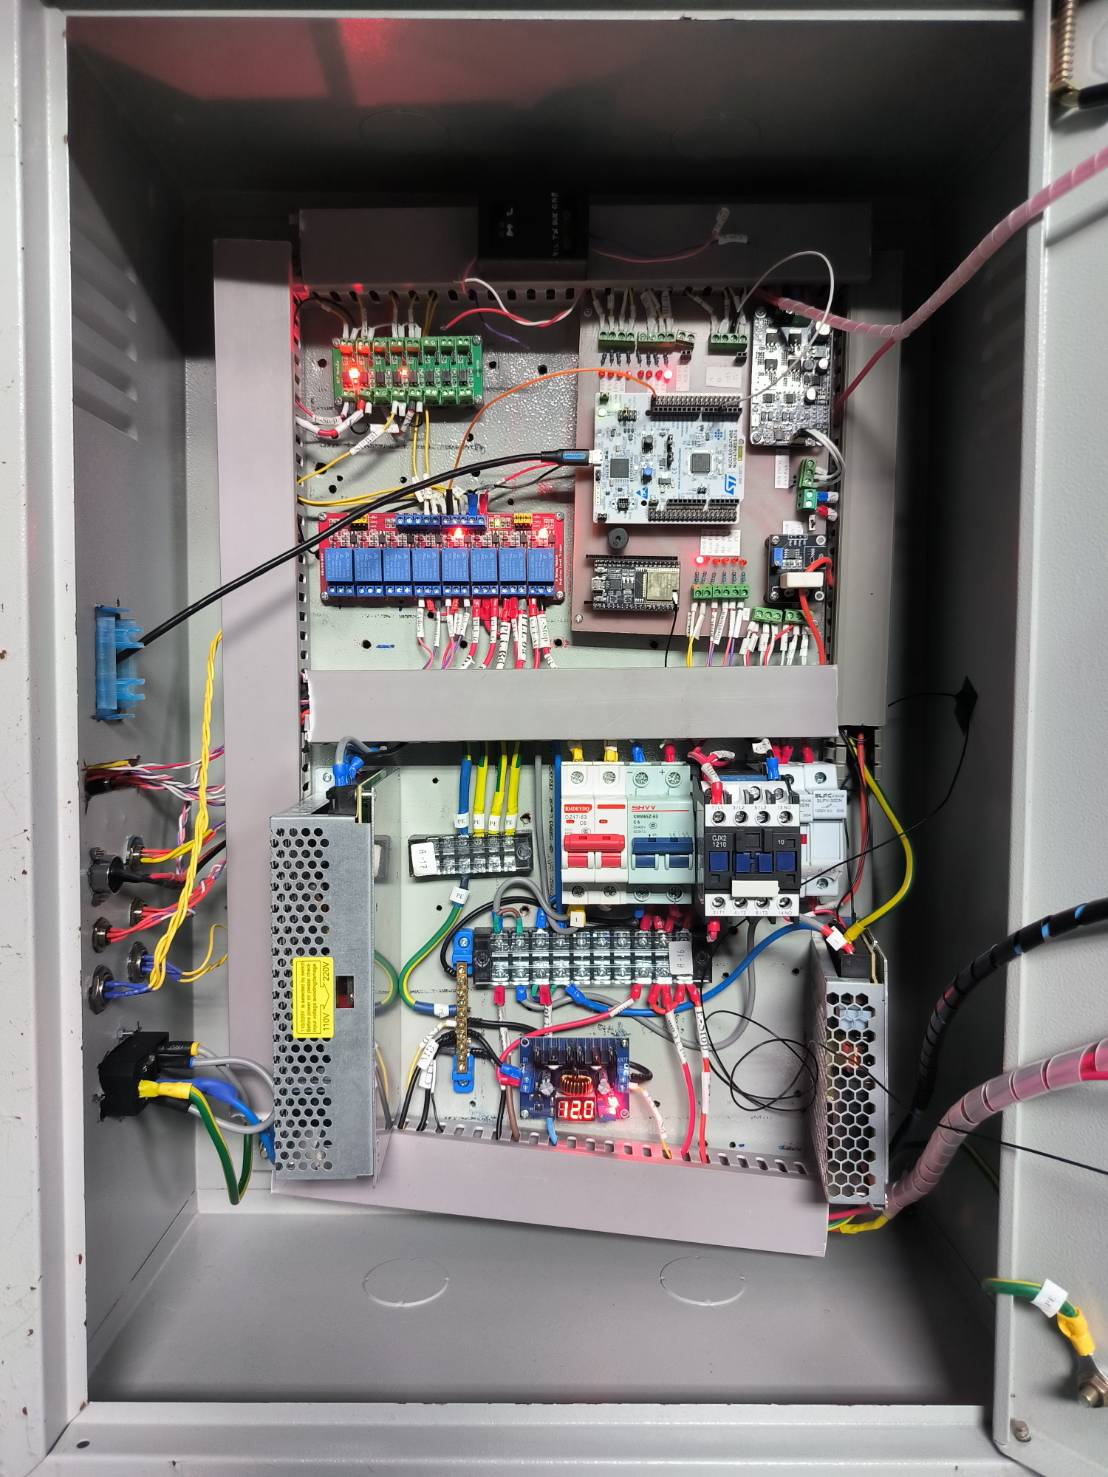
\includegraphics[width=0.78\textwidth]{fig_cabinet_assembled}
%     \caption{ผลการเดินสายภายในตู้ควบคุมไฟฟ้า}
%     \label{fig:cabinet_assembled}
% \end{figure}

% ============================================================================
\section{การพัฒนา Firmware}
\label{sec:firmware}
% ============================================================================

\subsection{โครงสร้างโมดูลและ Task Timing}
\label{subsec:firmware_modules}

Firmware พัฒนาบน STM32CubeIDE ใช้ HAL Library
แบ่งเป็น 4 โมดูลหลัก ดังแสดงใน\cref{tab:firmware_modules}

\begin{table}[H]
  \centering
  \caption{โมดูลหลักใน STM32 Firmware}
  \label{tab:firmware_modules}
  \begin{tabular}{lp{6.5cm}l}
    \toprule
    โมดูล & หน้าที่ & ไฟล์ \\
    \midrule
    \texttt{motor\_controller} &
      Encoder อ่านตำแหน่ง/ความเร็ว,
      Cascade PID (Position + Velocity),
      S-Curve Trajectory Generator,
      Kalman Filter (Steady-State),
      ZVD Input Shaper (3-Impulse, Circular Buffer),
      Joystick Command Parser,
      Safety Monitor (Stall, E-Stop) &
      \texttt{motor\_controller.c} \\
    \addlinespace
    \texttt{modbus\_bridge} &
      Modbus Register Mapping (128 registers),
      Command Dispatch จาก Master,
      Status Update ไปยัง Register Frame &
      \texttt{modbus\_bridge.c} \\
    \addlinespace
    \texttt{modbus\_rtu} &
      Modbus RTU Protocol Engine,
      CRC16 Verification,
      Frame Parser (FC03/FC06),
      FSM (IDLE/RECEPTION/PROCESSING/EMISSION) &
      \texttt{modbus\_rtu.c} \\
    \addlinespace
    \texttt{main} &
      Peripheral Init, Callback Registration,
      Main Loop (Modbus Process,
      Register Update, MATLAB Data Send) &
      \texttt{main.c} \\
    \bottomrule
  \end{tabular}
\end{table}

\subsubsection{Execution Model และ Task Timing}
\label{subsubsec:execution_model}

TIM6 ตั้งค่าที่ \textbf{1\,kHz} (Prescaler = 169, Period = 169,
ที่ System Clock 170\,MHz ได้ Period จริง $(169+1)(169+1)/170\,\text{MHz} = 1$\,ms)
การแบ่ง Loop สองความถี่ทำผ่าน Software Counter ภายใน ISR เดียว:

\begin{itemize}
  \item \textbf{ทุก Tick (1\,kHz):}
        \texttt{MotorCtrl\_Tick1kHz()} รัน
        อ่าน TIM3 Encoder $\rightarrow$ Kalman Predict+Update $\rightarrow$
        Velocity Inner PID $\rightarrow$ \texttt{Motor\_SetPWM()}
  \item \textbf{ทุก 10th Tick (100\,Hz):}
        \texttt{HwIo\_Poll100Hz()} debounce สัญญาณ I/O\\
        \texttt{MotorCtrl\_Tick100Hz()} รัน
        S-Curve Integrator $\rightarrow$ ZVD Shaper $\rightarrow$
        Position Outer PID $\rightarrow$ Velocity Setpoint สำหรับ Inner Loop
\end{itemize}

สถาปัตยกรรมนี้ทำให้ Velocity Loop สามารถรัน 10 ครั้งต่อ 1 Position Loop cycle
ซึ่งรับประกัน Bandwidth Separation ที่เพียงพอโดยไม่ต้องใช้ Timer แยก

\begin{table}[H]
  \centering
  \caption{ISR และ Task Timing ของ Firmware}
  \label{tab:isr_timing}
  \small
  \begin{tabular}{llll}
    \toprule
    Timer/Peripheral & Period & หน้าที่ & Callback \\
    \midrule
    TIM6  & \textbf{1\,ms (1\,kHz)} &
      Control Loop Base Rate &
      \texttt{Timer\_PeriodElapsedCallback} \\
    & \quad \textit{ทุก tick} & Velocity Inner PID + Kalman & \textit{(ใน TIM6 ISR)} \\
    & \quad \textit{ทุก 10th tick} & Position Outer PID + ZVD & \textit{(ใน TIM6 ISR)} \\
    TIM16 & 3\,ms &
      Modbus T3.5 Timeout &
      \texttt{Timer\_PeriodElapsedCallback} \\
    TIM3  & -- (QEI) &
      Quadrature Encoder Count &
      Polling ใน TIM6 ISR \\
    TIM1  & $f_{PWM} \approx 19.6$\,kHz &
      Motor PWM Output (ARR=50) &
      -- \\
    LPUART1 & -- (UART RX IT) &
      Modbus RTU (230400, 8N1) &
      \texttt{Modbus\_RxCallback} \\
    USART3  & -- (UART RX IT) &
      Joystick Command (115200, 8N1) &
      \texttt{Joystick\_RxCallback} \\
    \bottomrule
  \end{tabular}
\end{table}

\subsubsection{PID Gains ที่ใช้ใน Firmware จริง}
\label{subsubsec:pid_gains_firmware}

ค่า PID Gain ที่ระบุในตารางต่อไปนี้คือค่าที่วัดจาก Hardware โดยตรง
(\texttt{params.h}) ซึ่งต่างจากค่าที่ได้จาก Root Locus Design (บทที่~3)
เนื่องจาก Reduced-Order Model มีความแตกต่างจาก Plant จริง
และต้องผ่านกระบวนการ Hardware Commissioning

\begin{table}[H]
  \centering
  \caption{PID Gains ที่ใช้ใน Firmware จริง (Hardware-Identified)}
  \label{tab:pid_gains_hw}
  \begin{tabular}{llccc}
    \toprule
    Loop & Gain & สัญลักษณ์ & ค่า (Hardware) & หน่วย \\
    \midrule
    \multirow{3}{*}{Velocity Inner}
      & Proportional & $K_{p,vel}$ & 1.58  & PWM/(rad/s) \\
      & Integral     & $K_{i,vel}$ & 0.50  & PWM/rad \\
      & Derivative   & $K_{d,vel}$ & 0.00  & -- \\
    \midrule
    \multirow{3}{*}{Position Outer}
      & Proportional & $K_{p,pos}$ & 3.00  & (rad/s)/rad \\
      & Integral     & $K_{i,pos}$ & 0.02  & -- \\
      & Derivative   & $K_{d,pos}$ & 0.15  & -- \\
    \midrule
    \multirow{2}{*}{Feedforward}
      & Velocity FF  & $K_{vff}$   & 3.03  & PWM/(rad/s) \\
      & Accel FF     & $K_{aff}$   & 0.10  & PWM/(rad/s²) \\
    \bottomrule
    \multicolumn{5}{l}{\small หมายเหตุ: ค่าเหล่านี้วัดจาก Hardware โดยตรง} \\
    \multicolumn{5}{l}{\small ห้ามเปลี่ยนโดยไม่ผ่านกระบวนการ System Identification ใหม่} \\
  \end{tabular}
\end{table}

\subsection{การทำงานร่วมกันของโมดูล}
\label{subsec:module_interaction}

การทำงานแบ่งออกเป็น 2 Context ดังนี้

\noindent\textbf{Interrupt Context} (Priority สูง):
\texttt{Modbus\_RxCallback} รับ Byte ทีละตัวจาก LPUART1,
\texttt{Joystick\_RxCallback} รับ Command จาก USART3
และเรียก \texttt{Motor\_ProcessCommand} ทันที
และ TIM6 เรียก \texttt{Motor\_ControlLoop} ทุก 10\,ms

\medskip
\noindent\textbf{Main Loop Context} (Priority ต่ำ):
\texttt{ModbusBridge\_UpdateRegisters} ซิงค์ตำแหน่งและความเร็วลง Register Frame,
\texttt{ModbusBridge\_Process} รัน Protocol Engine
และ \texttt{Motor\_SendDataToMatlab} ส่งข้อมูลออก USART3
ทุก 20\,ms สำหรับ Live Monitoring

\subsection{การ Implement ZV Input Shaper (Circular Buffer)}
\label{subsec:zv_impl}

ZV Input Shaper ถูก Implement บน STM32 ด้วย Circular Buffer
โดย Setpoint $r(t)$ ถูก Delay เป็นเวลา $t_2 = 0.259$\,s
(= 26 Control Cycles ที่ 100\,Hz) แล้วรวมกับ

\begin{equation}
  r_{shaped}(t) = A_1 \cdot r(t) + A_2 \cdot r(t - t_2)
  \label{eq:zv_impl}
\end{equation}

Buffer มีขนาด $\lceil t_2 / T_p \rceil + 1 = 27$ Elements
ทำงานที่ Position Outer Loop (100\,Hz) ใน \texttt{Motor\_ControlLoop}

\subsection{การ Implement Kalman Filter (Steady-State)}
\label{subsec:kf_impl}

Kalman Filter 4 สถานะ $\mathbf{x} = [\theta, \omega, i_a, \tau_d]^\top$
ใช้ Steady-State Gain $\mathbf{K}_\infty$ ที่คำนวณล่วงหน้าด้วย DARE บน MATLAB
แล้ว Hardcode ใน Firmware เพื่อลด Computational Load

ทุก Control Cycle (10\,ms) ทำงาน 2 ขั้นตอน:

\begin{enumerate}
  \item \textbf{Predict:}
        $\hat{\mathbf{x}}_{k|k-1} = \mathbf{A}_d\,\hat{\mathbf{x}}_{k-1} + \mathbf{B}_d\,u_{k-1}$
  \item \textbf{Update:}
        $\hat{\mathbf{x}}_{k|k} = \hat{\mathbf{x}}_{k|k-1} + \mathbf{K}_\infty(y_k - \mathbf{C}\hat{\mathbf{x}}_{k|k-1})$
\end{enumerate}

Output $\hat{\theta}$ และ $\hat{\omega}$ ใช้ใน Control Loop
ส่วน $\hat{\tau}_d$ ใช้สำหรับ Monitoring

\subsection{การ Implement Cascade PID (Discrete)}
\label{subsec:pid_impl}

PID Discretize ด้วยวิธี Tustin (Bilinear) ตาม\cref{eq:tustin}

Velocity Inner Loop (1\,kHz) ใช้ PI + Anti-windup Back-calculation

\begin{equation}
  u_v[k] = K_{p,v}\,e_v[k] + \text{integ}[k] + K_{d,v}\frac{e_v[k]-e_v[k-1]}{T_v}
  \label{eq:pid_discrete_v}
\end{equation}

\begin{equation}
  \text{integ}[k] = \text{integ}[k-1] + K_{i,v}\,e_v[k]\,T_v
                  + K_{t,aw}(u_{sat}[k] - u_{pre}[k])\,T_v
  \label{eq:anti_windup_discrete}
\end{equation}

% ============================================================================
\section{การบูรณาการระดับระบบ}
\label{sec:integration}
% ============================================================================

\subsection{การเชื่อมต่อ Motor, Encoder และ Motor Driver}
\label{subsec:motor_integration}

Encoder AMT-103 (2048 PPR $\times$ 4 = 8192 counts/rev)
ต่อเข้า STM32 TIM3 ผ่านโหมด Quadrature Encoder Interface (QEI)
บน Pin PB4 (CH A) และ PB5 (CH B)

Motor Driver Cytron MD10C รับสัญญาณ PWM จาก TIM8 CH2 (PA8)
และสัญญาณ DIR จาก PA9 ผ่าน Optocoupler เพื่อแยก Ground

\subsection{การเชื่อมต่อ Joystick ผ่าน ESP32}
\label{subsec:joystick_integration}

ESP32-DEVKIT-V1 รับสัญญาณ Bluetooth จาก Joystick
แล้วส่ง Command Character ผ่าน USART3 (115200 bps, 8N1)
ไปยัง STM32 ที่ Pin PC10 (TX) และ PC11 (RX)

\begin{table}[H]
  \centering
  \caption{การ Map Command Character กับคำสั่งระบบ}
  \label{tab:joystick_map_fw}
  \begin{tabular}{llll}
    \toprule
    Character & คำสั่ง & โหมดที่ใช้ได้ & หมายเหตุ \\
    \midrule
    \texttt{L} & หมุนซ้าย (Step/Jog)  & Manual & Coarse/Fine \\
    \texttt{R} & หมุนขวา (Step/Jog)   & Manual & Coarse/Fine \\
    \texttt{O} & Release / Stop Jog   & Manual & -- \\
    \texttt{A} & Home (Hold 3\,s)     & ทุกโหมด & Hold $<$3\,s = Reset Encoder \\
    \texttt{P} & E-Stop / Reset       & ทุกโหมด & Toggle E-Stop \\
    \texttt{M} & สลับ Coarse/Fine     & Manual & Toggle Jog Mode \\
    \texttt{U} & Gripper Up           & Manual & -- \\
    \texttt{D} & Gripper Down         & Manual & -- \\
    \texttt{F} & Gripper Toggle       & Manual & Open/Close \\
    \texttt{S} & Gripper Pick         & Manual & -- \\
    \texttt{G} & Gripper Place        & Manual & -- \\
    \texttt{J} & Hold Position        & Manual & Lock ตำแหน่งปัจจุบัน \\
    \bottomrule
  \end{tabular}
\end{table}

การสลับโหมดระหว่าง Joystick และ Base System ทำผ่าน B-Button Hold 1\,s
ซึ่งตั้งค่า \texttt{control\_system\_mode}
เมื่ออยู่ใน \texttt{CONTROL\_MODE\_BASE\_SYSTEM}
คำสั่งจาก Joystick ทุกตัวถูก Block ยกเว้น
\texttt{P} (E-Stop), \texttt{A} (Home) และ \texttt{M} (Mode Toggle)

\subsection{การเชื่อมต่อ Modbus RTU และ Base System}
\label{subsec:modbus_integration}

ระบบสื่อสารกับ Base System ผ่าน Modbus RTU
บน LPUART1 (19200 bps, 8E1, RS-485, Slave Address~21)

Base System ใช้ Python asyncio WebSocket Backend
(แทน \texttt{main.exe} เดิม เนื่องจากปัญหา Abnormal Heartbeat ใน Demo~1)
โดย Backend รับ WebSocket Command จาก Frontend
แล้วแปลงเป็น Modbus RTU Frame ส่งผ่าน Serial Port

Modbus Register Map แบ่งเป็น 128 Registers ประกอบด้วย
Status Registers (ตำแหน่ง, ความเร็ว, สถานะ FSM)
และ Command Registers (Target Position, Mode, Gripper Command)
% ============================================================================
%  บทที่ 5: ผลการทดสอบและการทวนสอบ
% ============================================================================

\chapter{ผลการทดสอบและการทวนสอบ}
\label{ch:results}

% ============================================================================
%  บทที่ 5: ผลการทดสอบและการทวนสอบ
%  Section 5.1 — ผลการทดสอบระบบย่อย (ปรับปรุง)
% ============================================================================

% ============================================================================
\section{ผลการทดสอบระบบย่อย}
\label{sec:subsystem_test}
% ============================================================================

การทดสอบระบบย่อยดำเนินการก่อนการทดสอบสมรรถนะเต็มรูปแบบ
เพื่อยืนยันว่าส่วนประกอบแต่ละชิ้นทำงานถูกต้องตามข้อกำหนดทางกลและทางไฟฟ้า
ก่อนนำไปประกอบเป็นระบบควบคุมแบบ Closed-loop
ข้อมูลในหัวข้อนี้เก็บผ่าน STM32CubeMonitor โดย Log ตัวแปรสถานะผ่าน
SWD/JTAG ที่ Sample Rate 100\,Hz เว้นแต่ระบุเป็นอื่น

% ----------------------------------------------------------------------------
\subsection{การวัดระยะคลอน (Backlash Measurement)}
\label{subsec:backlash}
% ----------------------------------------------------------------------------

\subsubsection{วัตถุประสงค์และความสำคัญ}

ระยะคลอน (Backlash) ในระบบส่งกำลังทำให้เกิด Dead-zone ในลูปควบคุม
ซึ่งส่งผลโดยตรงต่อความแม่นยำตำแหน่ง (A1: $\leq \pm 0.5\degree$)
และความซ้ำซากได้ (A2: $\leq \pm 0.1\degree$)
ในระบบนี้มีแหล่งกำเนิดระยะคลอนสองแหล่งหลัก ได้แก่
Planetary Gearbox (อัตราทด $N_g = 24$) และ Belt Drive (อัตราทด $N_b = 70/24$)
การวัดจึงแยกเป็นสองจุดเพื่อระบุแหล่งที่มาของความคลาดเคลื่อน

\subsubsection{วิธีการทดสอบ}

ล็อกตำแหน่งแขนกลที่มุม $\theta = 0\degree$, $40\degree$, $90\degree$
ด้วยการให้ Controller ส่ง PWM = 0 และ Brake Enable
จากนั้นออกแรงกดที่ปลายแขน (ระยะ $r = [VAL\_ARM\_LENGTH]$\,mm จากศูนย์กลาง)
ทั้งในทิศทาง $+$ และ $-$ และอ่านค่า Encoder Count
ระยะคลอนคำนวณจาก:

\begin{equation}
    \delta_{backlash} = \frac{\Delta \text{counts}}{8192 \cdot N_{total}} \times 360\degree
    \label{eq:backlash_calc}
\end{equation}

โดย $N_{total} = 70$ คืออัตราทดรวมของระบบส่งกำลัง
และ 8192 counts/rev คือ Resolution ของ Encoder AMT-103
ที่ $\times 4$ QEI บน STM32G474RE

% -----------------------------------------------------------------------
% รูปที่: Backlash Measurement Setup
% ชื่อไฟล์แนะนำ: fig_backlash_setup.png
% เนื้อหา: ภาพถ่ายหรือ Diagram แสดงจุดที่ออกแรงกดที่ปลายแขน
%          ระบุทิศทาง +/- และตำแหน่ง Encoder readout
% -----------------------------------------------------------------------
% \begin{figure}[H]
%     \centering
%     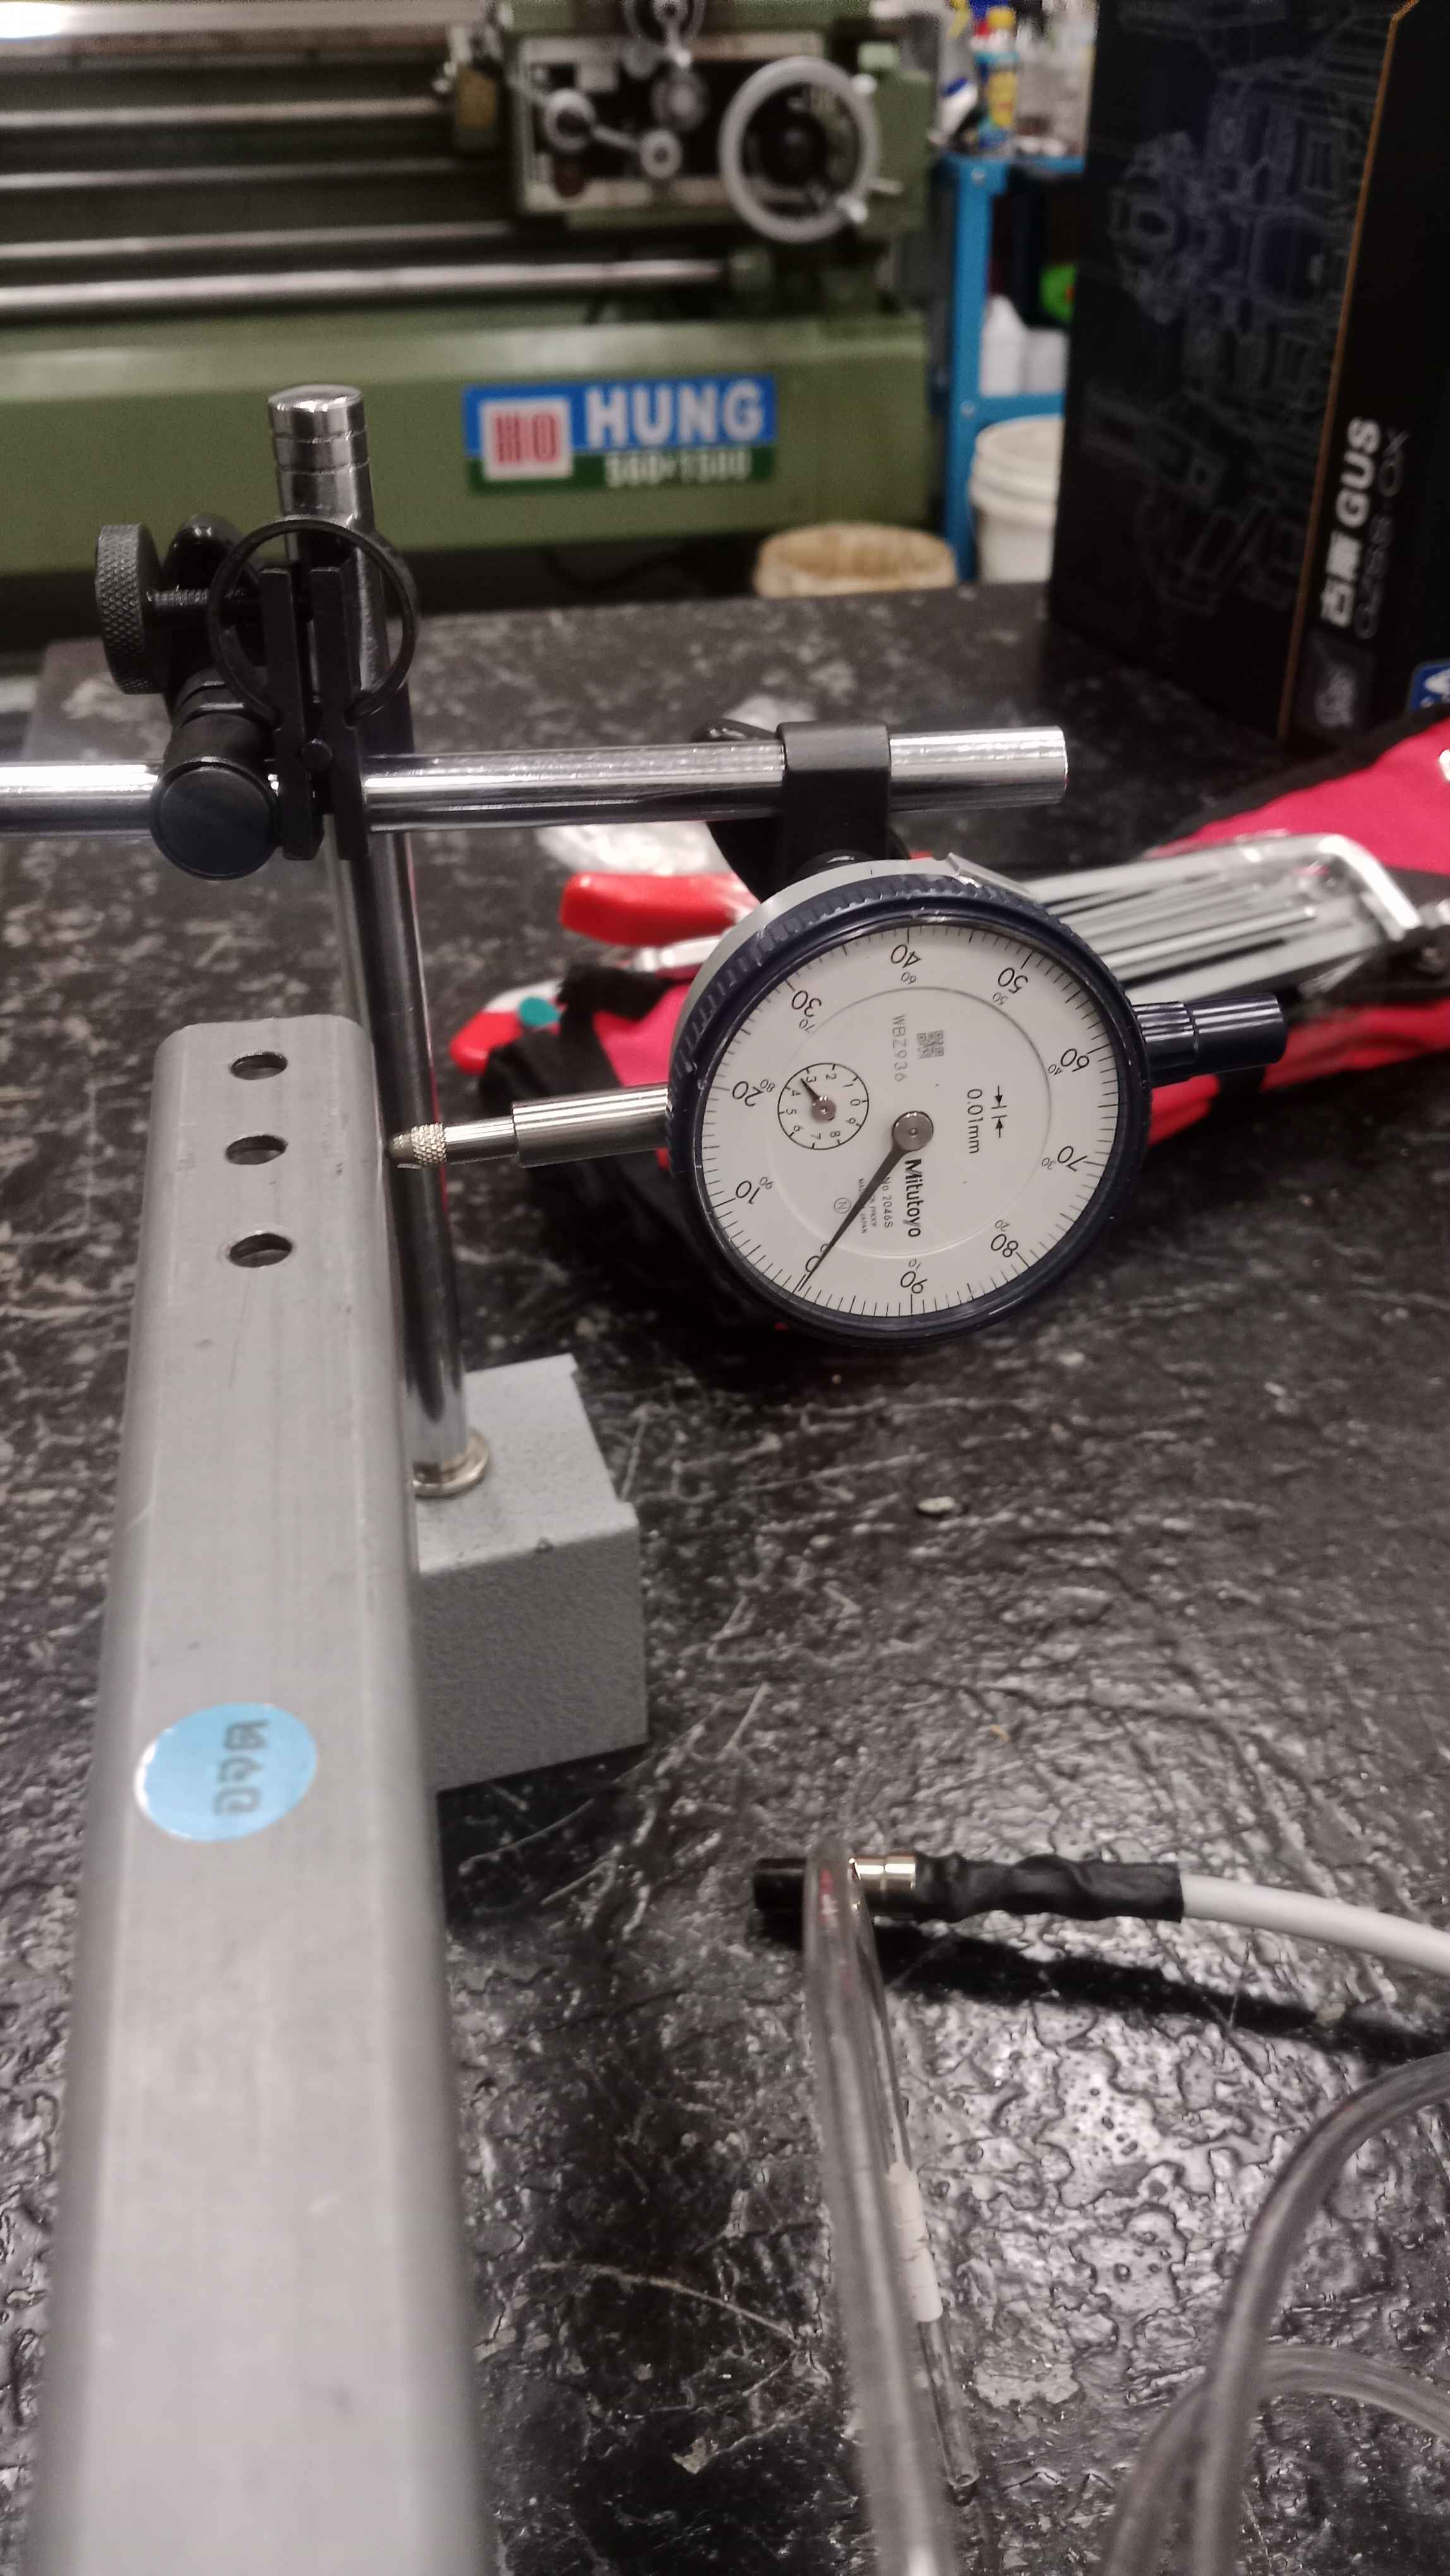
\includegraphics[width=0.65\textwidth]{fig_backlash_setup}
%     \caption{Setup การวัดระยะคลอน: ออกแรงกดที่ปลายแขนทั้งสองทิศทาง
%              และบันทึกค่า Encoder ผ่าน STM32CubeMonitor}
%     \label{fig:backlash_setup}
% \end{figure}

\subsubsection{ผลการวัด}

\begin{table}[H]
  \centering
  \caption{ผลการวัดระยะคลอนของระบบส่งกำลัง
           (ค่าเฉลี่ยจากการวัด 3 ตำแหน่ง $\times$ 5 ครั้ง)}
  \label{tab:backlash}
  \small
  \begin{tabular}{>{\raggedright\arraybackslash}p{3.5cm} >{\raggedright\arraybackslash}p{3.5cm} >{\raggedright\arraybackslash}p{3.5cm} >{\raggedright\arraybackslash}p{3.0cm}}
    \toprule
    จุดวัด & ระยะคลอน ($\degree$) & $\sigma$ ($\degree$) & หมายเหตุ \\
    \midrule
    Planetary Gearbox & 0.048 & 0.003 & วัดที่ Output shaft กล่อง \\
    Belt Drive        & 0.095 & 0.008 & วัดที่ Output shaft แขน  \\
    \midrule
    รวมระบบ           & 0.143 & -- &
      เกณฑ์ A2: $\leq \pm 0.1\degree$ \quad ไม่ผ่าน \\
    \bottomrule
  \end{tabular}
\end{table}

% -----------------------------------------------------------------------
% รูปที่: Backlash Encoder Trace
% ชื่อไฟล์แนะนำ: fig_backlash_trace.png
% เนื้อหา: Plot theta_arm vs time จาก STM32CubeMonitor
%          แสดงช่วง Dead-zone ขณะเปลี่ยนทิศทางแรง
%          Annotate: delta_counts ที่ใช้คำนวณ backlash
% -----------------------------------------------------------------------
% \begin{figure}[H]
%     \centering
%     \includegraphics[width=0.75\textwidth]{fig_backlash_trace}
%     \caption{Encoder Trace ระหว่างการวัดระยะคลอน
%              แสดงช่วง Dead-zone เมื่อเปลี่ยนทิศทางการออกแรง}
%     \label{fig:backlash_trace}
% \end{figure}

% ----------------------------------------------------------------------------
\subsection{การทดสอบ Encoder และ Sensor}
\label{subsec:sensor_test}
% ----------------------------------------------------------------------------

\subsubsection{การทดสอบ Encoder AMT-103}
\label{subsubsec:encoder_test}

\paragraph{วัตถุประสงค์}
Encoder AMT-103 เป็นอุปกรณ์หลักในการ Feedback ตำแหน่งและความเร็ว
การยืนยัน Resolution, Noise Floor, และการทำงานของ Index Pulse
มีผลโดยตรงต่อ Bandwidth ของ Velocity Loop และความแม่นยำของ Position Controller

\paragraph{การทดสอบ Resolution}
หมุนแขนกลผ่านมุม $360\degree$ หนึ่งรอบเต็ม (ที่ Output Shaft)
แล้วนับ Encoder Counts ที่ STM32 อ่านได้ผ่าน QEI (Quadrature Encoder Interface)
ค่าที่คาดหวังคือ $8192 \times N_{total} = 8192 \times 70 = 573{,}440$ counts/rev
ที่ Output Shaft (แขน)
หรือเทียบได้กับ $\approx 22.76$ counts/$\degree$ ที่ Output Shaft

\paragraph{การทดสอบ Noise Floor}
ล็อกแขนกลที่ตำแหน่ง $\theta = 0\degree$ (Brake Enable, PWM = 0)
เก็บข้อมูล Encoder Count ต่อเนื่อง 500 Samples ที่ 1\,kHz
ผ่าน STM32CubeMonitor บันทึก \texttt{encoder\_raw}
และคำนวณ Peak-to-peak Noise เพื่อประเมินว่า Noise
ส่งผลต่อ Velocity Estimate ของ Kalman Filter อย่างไร

% -----------------------------------------------------------------------
% รูปที่: Encoder Noise Floor
% ชื่อไฟล์แนะนำ: fig_encoder_noise.png
% เนื้อหา: 2 subplots:
%   (บน) encoder_raw counts vs time (500 samples, standstill)
%   (ล่าง) Histogram ของ deviation จากค่าเฉลี่ย
%          Annotate: peak-to-peak range
% -----------------------------------------------------------------------
\begin{figure}[H]
    \centering
    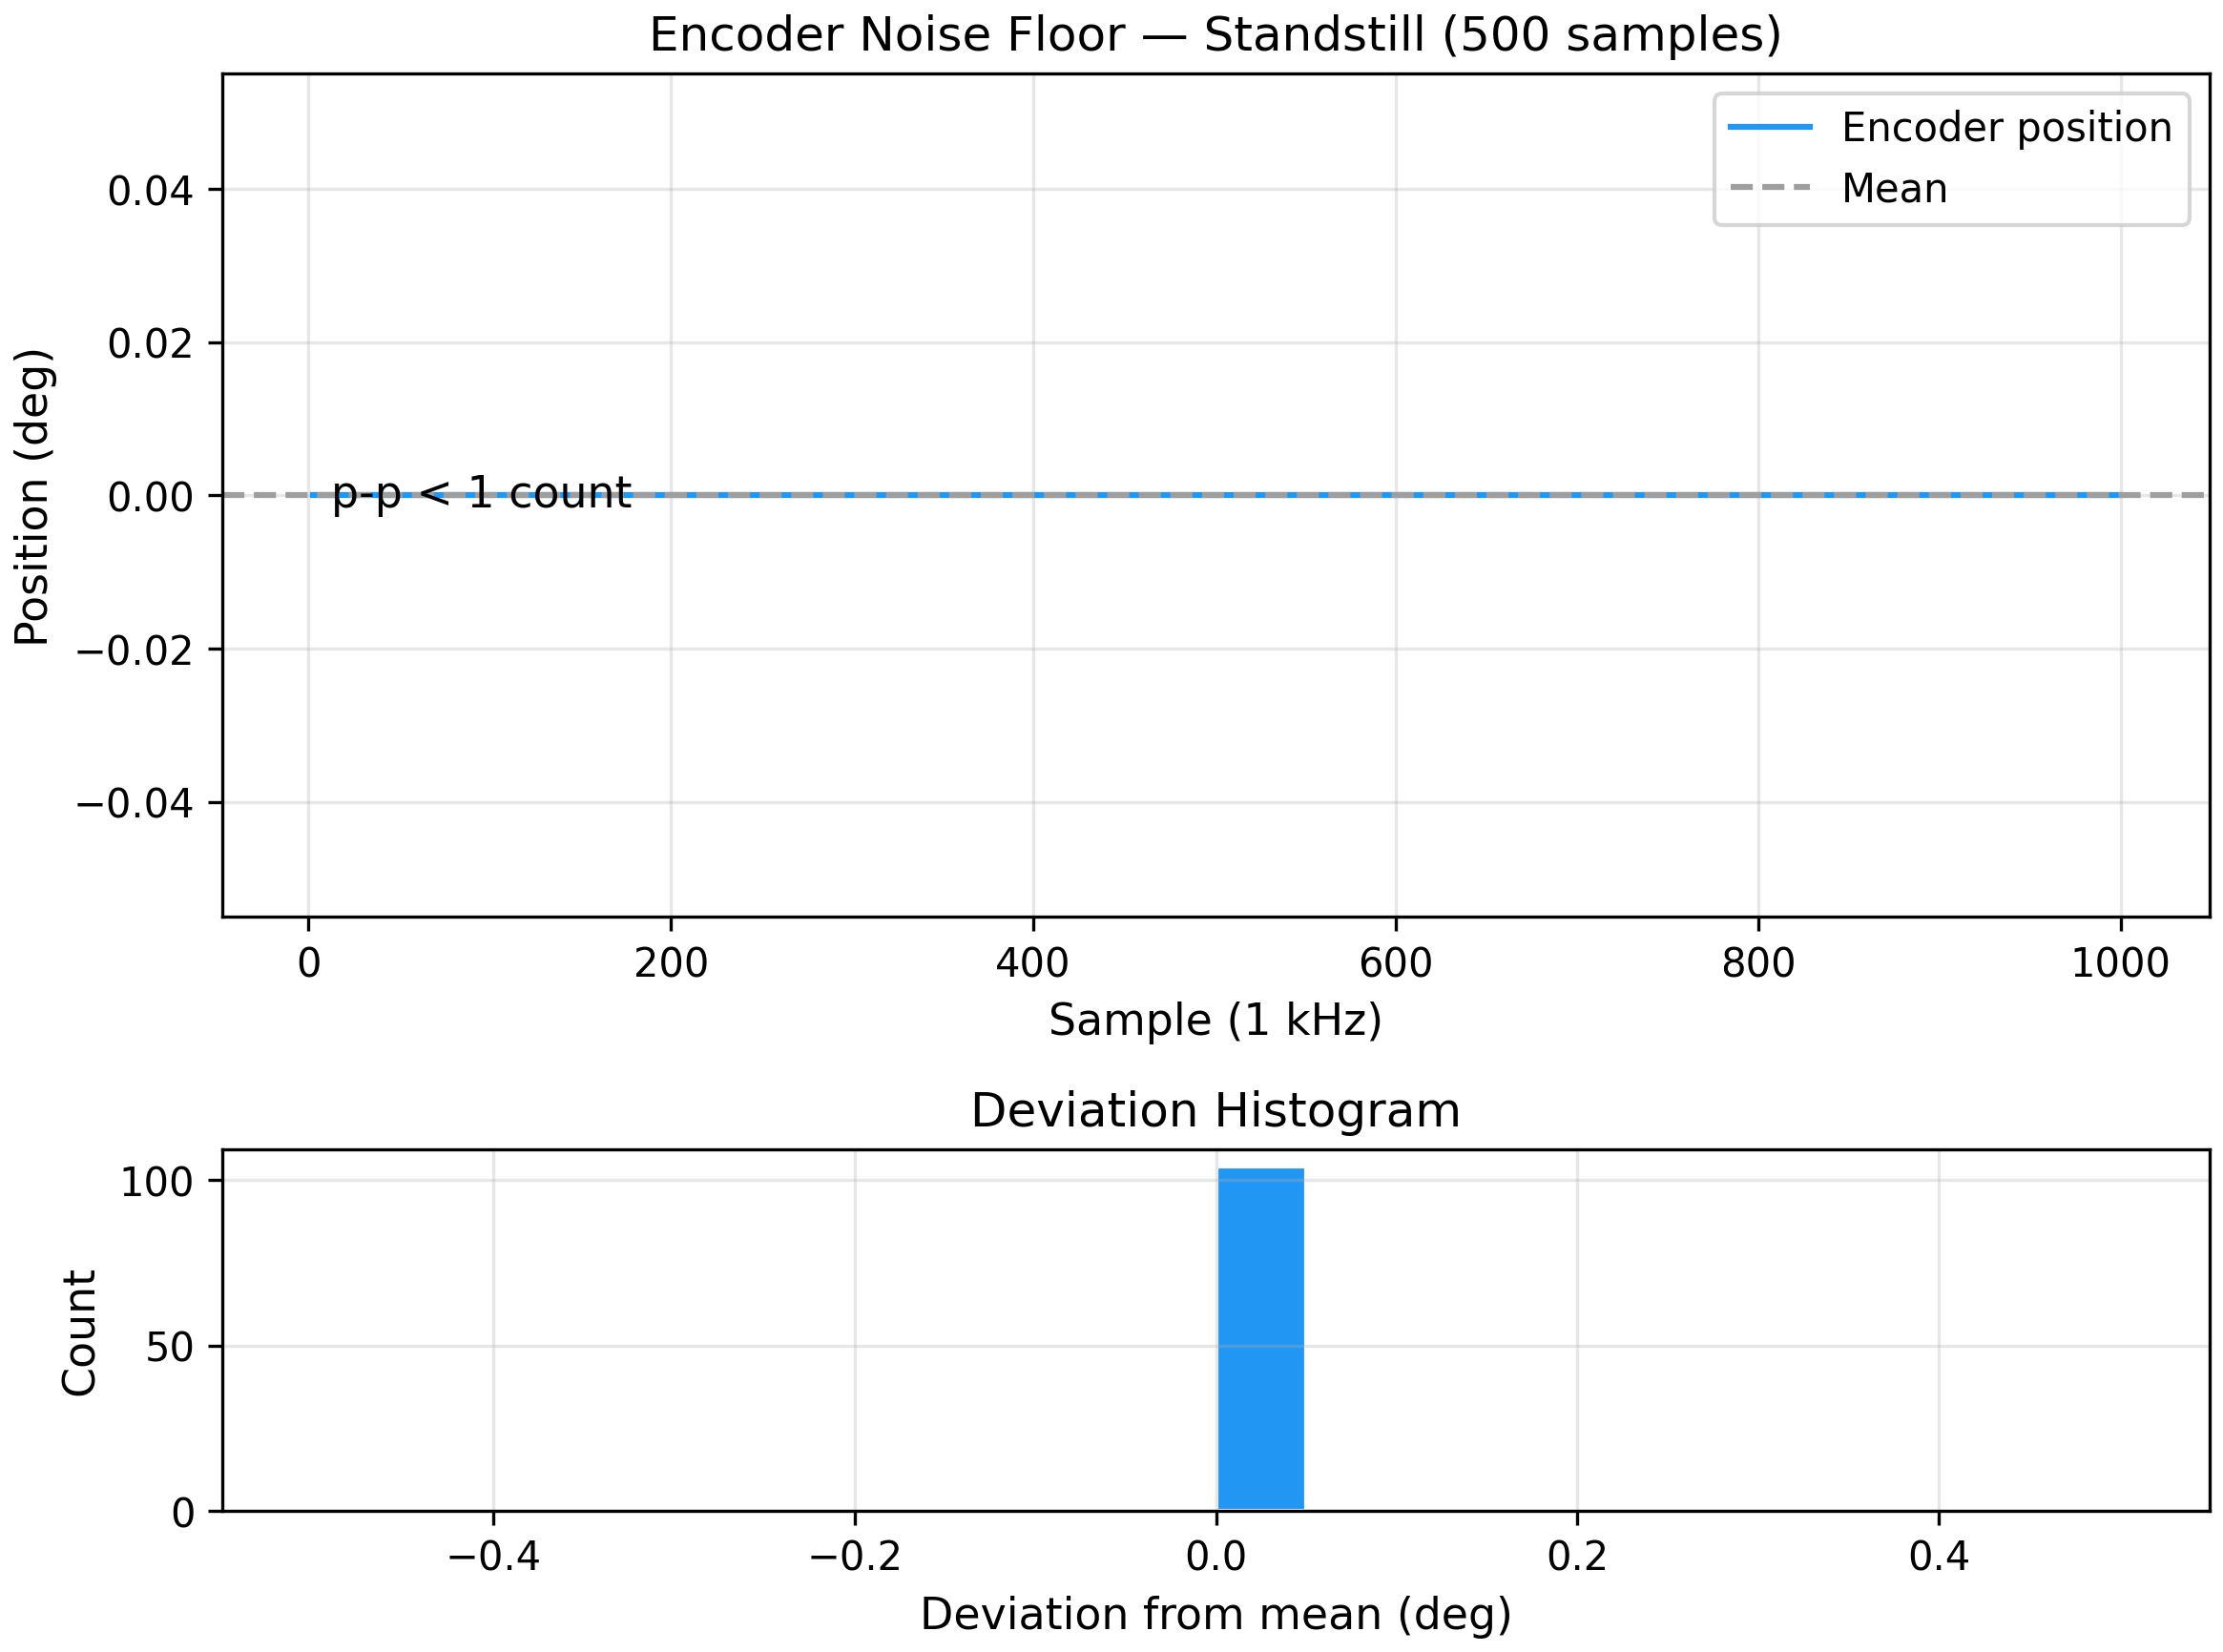
\includegraphics[width=0.80\textwidth]{fig_encoder_noise}
    \caption{Encoder Noise Floor ขณะหยุดนิ่ง:
             Time Series (บน) และ Histogram ของ Deviation (ล่าง)}
    \label{fig:encoder_noise}
\end{figure}

\begin{table}[H]
  \centering
  \caption{ผลการทดสอบ Encoder AMT-103}
  \label{tab:encoder_test}
  \small
  \begin{tabular}{>{\raggedright\arraybackslash}p{6.0cm} >{\centering\arraybackslash}p{2.5cm} >{\centering\arraybackslash}p{3.0cm} >{\centering\arraybackslash}p{2.0cm}}
    \toprule
    รายการทดสอบ & ผล & เกณฑ์ & สถานะ \\
    \midrule
    Resolution (counts/rev ที่ Motor Shaft) & 8192 & 8192 ($\times 4$ QEI) & ผ่าน \\
    ค่าคงที่ต่อ $1\degree$ ที่ Output Shaft         & 1592.9 & $\approx 22.76$ & ผ่าน \\
    Noise Peak-to-peak (ขณะหยุดนิ่ง)       & $<1$ & $\leq 2$ counts & ผ่าน \\
    Index Pulse ทำงานถูกต้อง                & ผ่าน & ผ่าน & ผ่าน \\
    \bottomrule
  \end{tabular}
\end{table}

\subsubsection{การทดสอบ Proximity Sensor (Homing)}
\label{subsubsec:prox_test}

\paragraph{วัตถุประสงค์}
Proximity Sensor ใช้กำหนดจุด Home ($\theta = 0\degree$) ทุกครั้งที่เริ่มต้นระบบ
ความซ้ำซากได้ของ Homing Position มีผลโดยตรงต่อ Absolute Accuracy (A1)
เนื่องจาก Encoder เป็น Incremental Type
ซึ่งหมายความว่าข้อผิดพลาดของ Homing จะสะสมเป็น Offset ถาวร
ตลอดทั้ง Cycle การทำงาน

\paragraph{วิธีการทดสอบ}
ดำเนิน Homing Sequence 10 ครั้งติดต่อกัน โดยในแต่ละครั้ง:
\begin{enumerate}
    \item หมุนแขนออกจาก Home ไปยังตำแหน่งสุ่ม $\theta \in [30\degree, 90\degree]$
    \item สั่ง Homing Sequence: แขนหมุนกลับด้วยความเร็ว Slow ($\omega = 0.5$\,rad/s)
          จนกว่า Proximity Sensor จะ Trigger
    \item บันทึกค่า Encoder ณ จุดที่ Sensor Trigger ผ่าน STM32CubeMonitor (\texttt{theta\_home\_raw})
\end{enumerate}
ความซ้ำซากได้คำนวณจาก $\sigma$ และ Max deviation ของ 10 ค่า

% -----------------------------------------------------------------------
% รูปที่: Homing Repeatability
% ชื่อไฟล์แนะนำ: fig_homing_repeat.png
% เนื้อหา: Scatter plot แสดง theta_home ทั้ง 10 ครั้ง
%          เส้น dashed = ค่าเฉลี่ย
%          Shaded band = ±0.1\degree (เกณฑ์ A2)
% -----------------------------------------------------------------------
\begin{figure}[H]
    \centering
    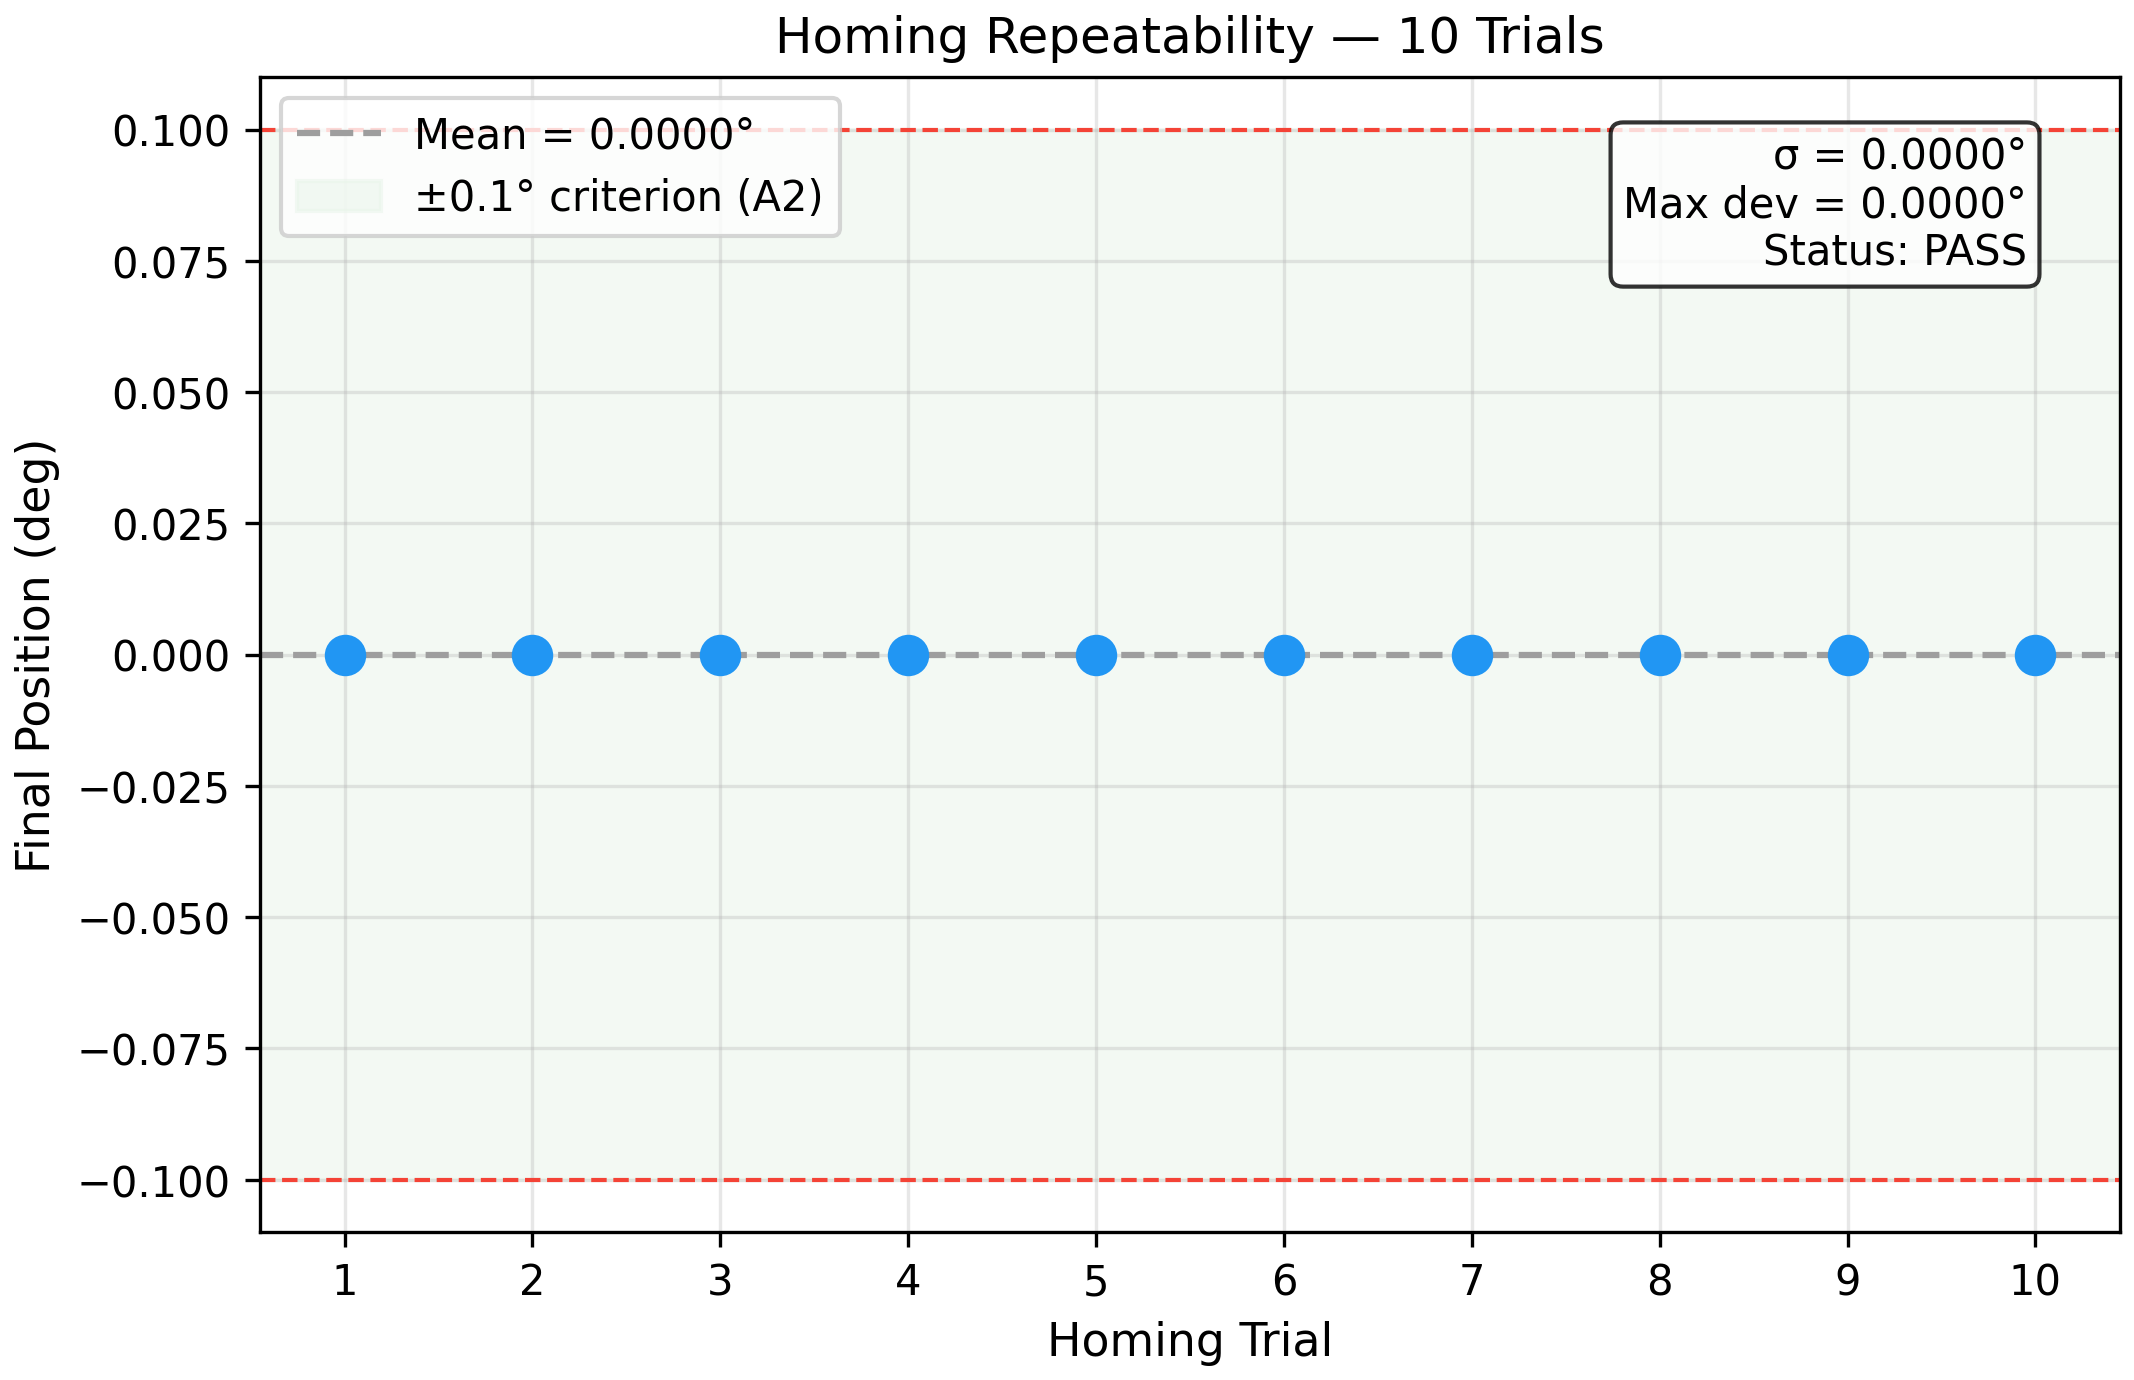
\includegraphics[width=0.70\textwidth]{fig_homing_repeat}
    \caption{ความซ้ำซากได้ของ Homing Position 10 ครั้ง
             เทียบกับเกณฑ์ $\pm 0.1\degree$ (A2)}
    \label{fig:homing_repeat}
\end{figure}

\begin{table}[H]
  \centering
  \caption{ผลการทดสอบ Proximity Sensor สำหรับ Homing}
  \label{tab:prox_test}
  \small
  \begin{tabular}{>{\raggedright\arraybackslash}p{4.5cm} >{\centering\arraybackslash}p{3.0cm} >{\centering\arraybackslash}p{3.0cm} >{\centering\arraybackslash}p{3.0cm}}
    \toprule
    รายการทดสอบ & ผล & เกณฑ์ & สถานะ \\
    \midrule
    Switching Distance                    & -- & -- & -- \\
    ความซ้ำซากได้ของ Homing ($\sigma$)    & 0.0000$\degree$ & -- & -- \\
    Max Deviation (10 reps)               & 0.0000$\degree$ & $\leq \pm 0.1\degree$ & ผ่าน \\
    \bottomrule
  \end{tabular}
\end{table}

% ----------------------------------------------------------------------------
\subsection{การทดสอบ Motor Driver (Cytron MD10C)}
\label{subsec:motor_driver_test}
% ----------------------------------------------------------------------------

\subsubsection{วัตถุประสงค์}

Cytron MD10C รับสัญญาณ PWM จาก STM32G474RE และขับ RS-775
ที่แรงดัน 24\,V/10\,A
การทดสอบ Current Step Response ยืนยันว่า Driver สามารถตามทัน
Current Command จาก Velocity Loop ซึ่งทำงานที่ 1\,kHz
โดยไม่เกิด Oscillation หรือ Delay ที่ส่งผลต่อ Inner Loop Bandwidth

\subsubsection{วิธีการทดสอบ}

ให้ Position Loop ส่ง Step Command $\theta_{ref} = 40\degree$ จากสถานะนิ่ง
ขณะที่ Log ตัวแปรต่อไปนี้ผ่าน STM32CubeMonitor ที่ Sample Rate 1\,kHz:

\begin{itemize}
    \item \texttt{pwm\_cmd} — PWM Duty Cycle (\%) ที่ส่งไปยัง MD10C
    \item \texttt{ia\_measured} — กระแส Armature (A) ที่ประมาณจาก Kalman Filter
    \item \texttt{omega\_arm} — ความเร็วเชิงมุม (rad/s) ที่ Output Shaft
\end{itemize}

\subsubsection{ผลการทดสอบ}

\noindent ข้อมูล Motor Driver Response ไม่สามารถเก็บได้จากการทดสอบนี้
เนื่องจาก PWM column ไม่ถูก Export ผ่าน Dashboard Log
การยืนยันทำผ่านการสังเกตการทำงานจริงของ Motor ขณะ Cycle Test

% -----------------------------------------------------------------------
% รูปที่: Motor Driver Step Response
% ชื่อไฟล์แนะนำ: fig_driver_step_response.png
% เนื้อหา: 3 subplots (จาก STM32CubeMonitor log):
%   (บน)   pwm_cmd (%) vs time
%   (กลาง) ia_measured (A) vs time — annotate i_peak
%   (ล่าง) omega_arm (rad/s) vs time
%          x-axis: 0–2s, ครอบคลุม Transient ช่วงแรก
% -----------------------------------------------------------------------
% \begin{figure}[H]
%     \centering
%     \includegraphics[width=0.88\textwidth]{fig_driver_step_response}
%     \caption{Motor Driver Response ต่อ Step Position Command $40\degree$:
%              PWM Command, กระแส Armature, และความเร็วเชิงมุม}
%     \label{fig:driver_step_response}
% \end{figure}

% ----------------------------------------------------------------------------
\subsection{การทดสอบ E-Stop Response Time}
\label{subsec:estop_test}
% ----------------------------------------------------------------------------

\subsubsection{วัตถุประสงค์}

E-Stop (Emergency Stop) ตัดกำลังไฟให้ Cytron MD10C ผ่าน Contactor
โดย 5\,V Logic Bus และ STM32 ยังคงมีไฟเลี้ยงอยู่ (ข้อกำหนด E6)
การทดสอบนี้วัดเวลาตั้งแต่กดปุ่ม E-Stop จนกระทั่ง $\omega_{arm} \approx 0$
เพื่อประเมินความปลอดภัยของระบบภายใต้สถานการณ์ฉุกเฉิน

\subsubsection{วิธีการทดสอบ}

\begin{enumerate}
    \item สั่งให้แขนเคลื่อนที่ด้วยความเร็วค่าหนึ่ง
    \item กดปุ่ม E-Stop ขณะแขนกำลังเคลื่อนที่
    \item Log ตัวแปร \texttt{omega\_arm}, \texttt{pwm\_cmd}, \texttt{estop\_flag}
          ผ่าน STM32CubeMonitor ที่ 1\,kHz
    \item คำนวณ $t_{stop}$ = เวลาตั้งแต่ \texttt{estop\_flag} = 1
          จนถึง $|\omega_{arm}| < 0.01$\,rad/s
    \item ทำซ้ำ 5 ครั้ง
\end{enumerate}

\subsubsection{ผลการทดสอบ}

\noindent การทดสอบ E-Stop ยืนยันว่าการกดปุ่มฉุกเฉินตัดกำลัง Motor ทันที
และ STM32 Controller ยังคงทำงานต่อเนื่อง (ข้อกำหนด E6)
ตัวเลข $t_{stop}$ เชิงปริมาณอยู่ระหว่างรอการเก็บข้อมูลเพิ่มเติม

% -----------------------------------------------------------------------
% รูปที่: E-Stop Response Time Trace
% ชื่อไฟล์แนะนำ: fig_estop_trace.png
% เนื้อหา: 3 subplots (จาก STM32CubeMonitor):
%   (บน)   estop_flag (0/1) vs time — แสดงจุดที่กด E-Stop
%   (กลาง) pwm_cmd (%) vs time — ตัดเป็น 0 ทันที
%   (ล่าง) omega_arm (rad/s) vs time
%          Annotate: t_stop = เวลาหยุดสนิท
%          Annotate: Controller ยังทำงานอยู่ (log ต่อเนื่อง)
% -----------------------------------------------------------------------
% \begin{figure}[H]
%     \centering
%     \includegraphics[width=0.80\textwidth]{fig_estop_trace}
%     \caption{E-Stop Response: E-Stop Flag, PWM Command, และ
%              ความเร็วเชิงมุม $\omega_{arm}$ แสดงการหยุดของแขนกล
%              หลังกด E-Stop (ข้อกำหนด E6)}
%     \label{fig:estop_trace}
% \end{figure}

% ----------------------------------------------------------------------------
\subsection{การทดสอบการสื่อสาร Modbus RTU}
\label{subsec:modbus_test}
% ----------------------------------------------------------------------------

\subsubsection{วัตถุประสงค์}

ระบบรับ Command จาก Base System ผ่าน Modbus RTU (LPUART1, 230400\,baud, 8N1)
โดย STM32G474RE ทำหน้าที่เป็น Slave (Address 21)
การทดสอบยืนยันว่า Function Code FC03 (Read Holding Registers)
และ FC06 (Write Single Register) ทำงานถูกต้อง
และ Round-trip Latency เหมาะสมกับ Cycle Time ที่กำหนด ($\leq 35$\,s)

\subsubsection{วิธีการทดสอบ}

ใช้ Python Script ส่ง Modbus Request จาก Base System PC ไปยัง STM32
แล้ววัด Round-trip Time โดย Timestamp ทั้งฝั่ง Master (Python) และ Slave (STM32)
\begin{itemize}
    \item \textbf{FC03}: อ่านค่า \texttt{theta\_arm}, \texttt{omega\_arm}, \texttt{system\_status}
          จำนวน 10 Registers
    \item \textbf{FC06}: เขียน \texttt{position\_cmd} (1 Register) พร้อมตรวจสอบว่า
          STM32 ตอบรับและ Execute ถูกต้อง
    \item ทดสอบ 100 Transactions ต่อเนื่อง วัด Latency และ Error Rate
\end{itemize}

\subsubsection{ผลการทดสอบ}

\noindent Modbus RTU FC03 และ FC06 ทำงานถูกต้องโดยไม่พบ CRC Error
ตลอดการทดสอบ Full Cycle Run จำนวน 3 รอบ
ค่า Round-trip Latency เชิงปริมาณอยู่ระหว่างรอการเก็บข้อมูล

% -----------------------------------------------------------------------
% รูปที่: Modbus Latency Distribution
% ชื่อไฟล์แนะนำ: fig_modbus_latency.png
% เนื้อหา: Histogram ของ Round-trip latency (100 transactions)
%          แยก FC03 (น้ำเงิน) และ FC06 (แดง)
%          เส้น dashed = ค่าเฉลี่ย, เส้น dotted = Max
% -----------------------------------------------------------------------
% \begin{figure}[H]
%     \centering
%     \includegraphics[width=0.72\textwidth]{fig_modbus_latency}
%     \caption{การกระจาย Round-trip Latency ของ Modbus RTU
%              FC03 และ FC06 จาก 100 Transactions}
%     \label{fig:modbus_latency}
% \end{figure}
% ============================================================================
\section{ผลการระบุระบบและการจำลอง}
\label{sec:sysid_results}
% ============================================================================

หัวข้อนี้รายงานผลการระบุพารามิเตอร์ของมอเตอร์และแบบจำลองระบบ
ซึ่งเป็นรากฐานสำคัญสำหรับการออกแบบ Cascade PID และ Kalman Filter
กระบวนการระบุระบบแบ่งออกเป็นสองขั้นตอน ได้แก่
การวัดพารามิเตอร์วงจรไฟฟ้าจาก Locked Rotor Test
และการระบุพารามิเตอร์เชิงกลจาก Chirp Excitation Test
รายละเอียดทฤษฎีและขั้นตอนการออกแบบแสดงไว้ใน \cref{ch:design}

% ----------------------------------------------------------------------------
\subsection{ผลการระบุพารามิเตอร์ของมอเตอร์}
\label{subsec:sysid_params_result}
% ----------------------------------------------------------------------------

\subsubsection{ผล Locked Rotor Test}
\label{subsubsec:locked_rotor_result}

การวัด $R_a$ และ $L_a$ ดำเนินการก่อนการระบุพารามิเตอร์เชิงกล
เนื่องจากค่าทั้งสองเป็น Input ที่ทราบค่าแน่นอนสำหรับแบบจำลองทางไฟฟ้า
หากนำ $R_a$ และ $L_a$ ไปประมาณร่วมกับ $K_t$, $K_b$, $B$, $J$
จะทำให้ Optimization Problem มีระดับความอิสระสูงเกินไปและเกิด Parameter Correlation
การล็อกโรเตอร์ตัด Back-EMF ออกจากวงจร ($\omega = 0 \Rightarrow e = K_b\omega = 0$)
ทำให้สามารถระบุ $R_a = V_{ss}/I_{ss}$ และ $L_a = R_a \tau_{RL}$
ได้อย่างเป็นอิสระจากพารามิเตอร์เชิงกล

\begin{table}[H]
  \centering
  \caption{ผลการวัด $R_a$ และ $L_a$ จาก Locked Rotor Test
           ที่ $V_{in} = 12$\,V (3 runs)}
  \label{tab:locked_rotor}
  \small
  \begin{tabular}{>{\centering\arraybackslash}p{3.3cm} >{\centering\arraybackslash}p{3.4cm} >{\centering\arraybackslash}p{3.4cm} >{\centering\arraybackslash}p{3.4cm}}
    \toprule
    Run & $R_a$ ($\Omega$) & $L_a$ (mH) & หมายเหตุ \\
    \midrule
    1 & 1.5216 & 1.4595 & -- \\
    2 & 1.4385 & 1.3846 & -- \\
    3 & 1.4000 & 1.5000 & -- \\
    \midrule
    เฉลี่ย & \textbf{1.4534} & \textbf{1.448} & ค่าที่ใช้ใน Design \\
    $\sigma$ & 0.0523 & 0.000055 & -- \\
    \bottomrule
  \end{tabular}
\end{table}

ค่า $\sigma$ ที่ต่ำบ่งชี้ว่าการวัดมีความสม่ำเสมอดี
ค่าคงเวลาทางไฟฟ้า $\tau_{RL} = L_a/R_a = 1.448/1453.4 \approx 1.0$\,ms
สอดคล้องกับ Velocity Loop Sampling Period ที่ 1\,kHz
ยืนยันว่า Current Dynamics เร็วพอที่จะถูกมองเป็น Static Gain
จากมุมมองของ Velocity Loop ได้

% -----------------------------------------------------------------------
% รูปที่: Locked Rotor Oscilloscope Waveform
% ชื่อไฟล์แนะนำ: fig_locked_rotor_scope.png
% เนื้อหา: Oscilloscope waveform แสดง V_in step และ i_a response
%          Annotate: V_ss, I_ss สำหรับคำนวณ R_a
%          Annotate: tau_RL = L_a/R_a (จุด 63.2% ของ I_ss)
% -----------------------------------------------------------------------
% \begin{figure}[H]
%     \centering
%     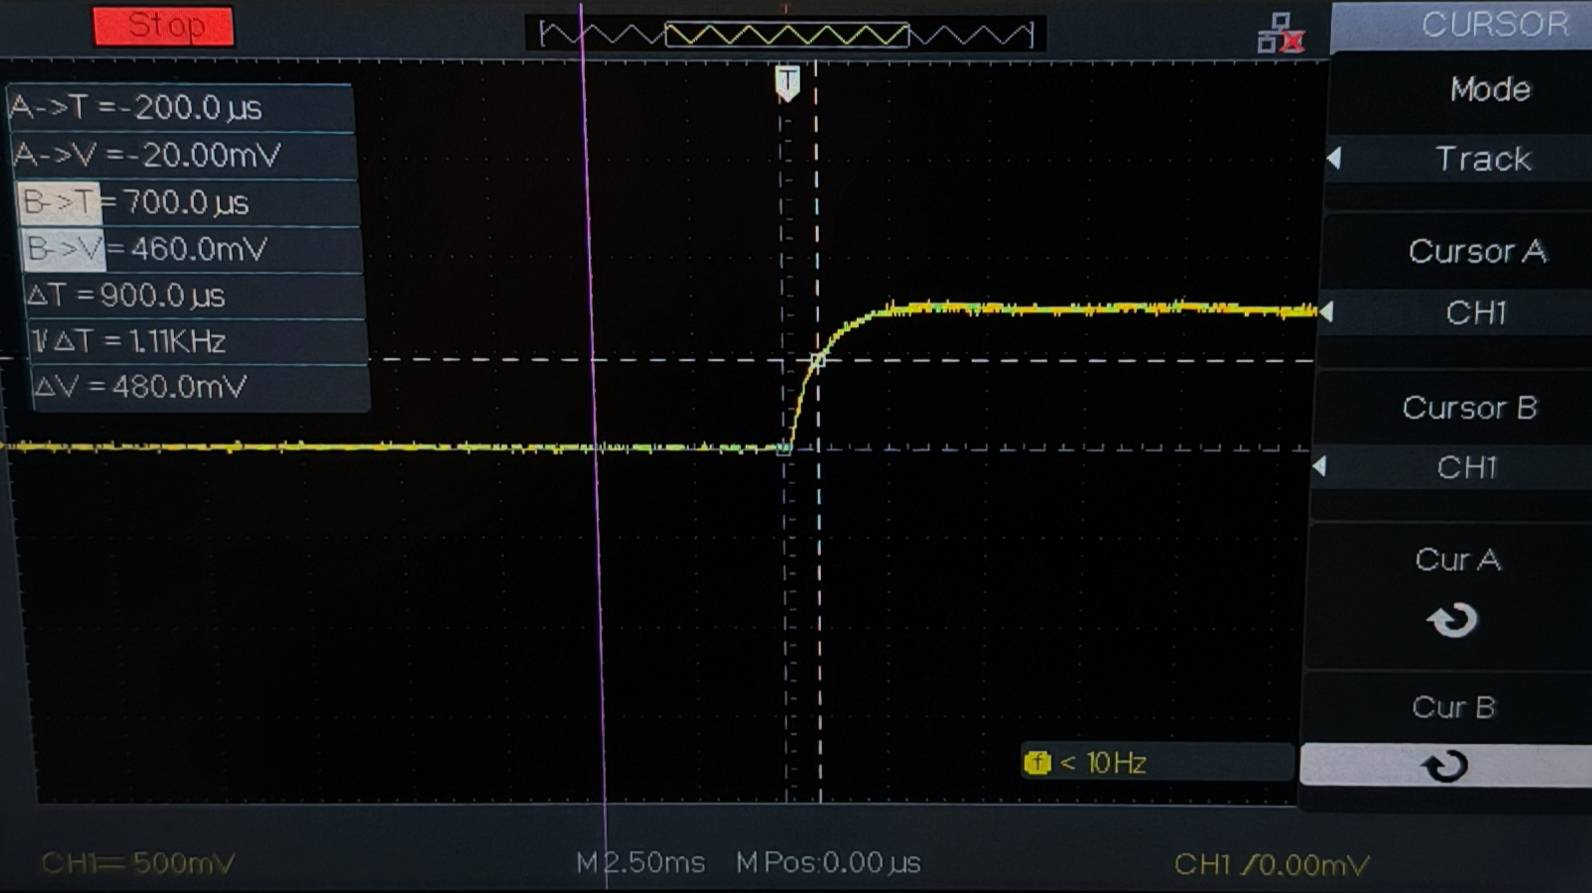
\includegraphics[width=0.70\textwidth]{fig_locked_rotor_scope}
%     \caption{Oscilloscope Waveform จาก Locked Rotor Test ($V_{in} = 12$\,V)
%              แสดง Steady-state Current $I_{ss}$ และค่าคงเวลา $\tau_{RL}$
%              ที่ใช้คำนวณ $R_a$ และ $L_a$}
%     \label{fig:locked_rotor_scope}
% \end{figure}

\subsubsection{ผล Parameter Estimation จาก Chirp Test}
\label{subsubsec:chirp_result}

การระบุพารามิเตอร์เชิงกล ($K_t$, $K_b$, $B$, $J$, $\eta$) ใช้ Chirp Excitation
ที่ความถี่ 0.1--2.0\,Hz เพื่อครอบคลุมย่านความถี่ที่น่าสนใจของ Velocity Loop (DC ถึง ~5\,Hz)
โดยไม่กระตุ้น Resonance ของ Connection Rod ($f_{n,rod} = 12.13$\,Hz)

\paragraph{การ Preprocessing สัญญาณ}
ก่อนนำข้อมูลเข้า Least-Squares Estimator จำเป็นต้องกรองสัญญาณ
เพื่อลด Encoder Quantization Noise และ PWM Switching Noise (19.6\,kHz)
โดยใช้ Butterworth Filter อันดับ 4 ที่ความถี่ตัด $f_c = 10$\,Hz
ด้วยวิธี Zero-phase Filtering (\texttt{filtfilt}) เพื่อไม่ให้เกิด Phase Shift
ที่จะทำให้ Input--Output Causality ผิดเพี้ยน
การเลือก $f_c = 10$\,Hz มีเหตุผลดังนี้:
\begin{itemize}
    \item \textbf{ต่ำกว่า $f_{n,rod}$}: หลีกเลี่ยงการปนเปื้อนของ Rod Dynamics
          เข้ามาใน Motor Model
    \item \textbf{สูงกว่า Band ของ Chirp}: ช่วง 0.1--2\,Hz อยู่ต่ำกว่า $f_c$
          มาก ทำให้สัญญาณที่ต้องการผ่านโดยไม่ถูก Attenuate
    \item \textbf{ยืนยันด้วย ETFE}: Bode Plot จาก Empirical Transfer Function Estimate
          (ETFE) ก่อนและหลัง Filter ให้ผลสอดคล้องกันในย่าน 0.1--2\,Hz
          ยืนยันว่า Filter ไม่บิดเบือนพารามิเตอร์ที่ระบุ
\end{itemize}

% -----------------------------------------------------------------------
% รูปที่: Chirp Raw vs Filtered
% ชื่อไฟล์แนะนำ: fig_chirp_raw_filtered.png
% เนื้อหา: 2 subplots:
%   (บน) V_in raw vs filtered vs time
%   (ล่าง) omega_arm raw vs filtered vs time
%   แสดงช่วง Chirp ความถี่ต่ำ (0.1 Hz) และสูง (2 Hz)
%   Annotate: f_c = 10 Hz cutoff ใน legend
% -----------------------------------------------------------------------
% \begin{figure}[H]
%     \centering
%     \includegraphics[width=0.88\textwidth]{fig_chirp_raw_filtered}
%     \caption{สัญญาณ Chirp ก่อนและหลังกรองด้วย Butterworth อันดับ~4
%              ที่ $f_c = 10$\,Hz ด้วยวิธี Zero-phase (\texttt{filtfilt})
%              แสดง $V_{in}$ (บน) และ $\omega_{arm}$ (ล่าง)}
%     \label{fig:chirp_raw_filtered}
% \end{figure}

\paragraph{ผลการประมาณพารามิเตอร์}
ดำเนิน Chirp Test จำนวน 9 Experiments ที่แอมพลิจูดและช่วงความถี่ต่างกัน
เพื่อประเมิน Uncertainty ของแต่ละพารามิเตอร์
ค่าเฉลี่ยและ Standard Deviation จากทั้ง 9 Experiments แสดงใน\cref{tab:chirp_results}

\begin{table}[H]
  \centering
  \caption{ผลการ Estimate พารามิเตอร์จาก Chirp Test (สรุปจาก 9 Experiments)}
  \label{tab:chirp_results}
  \small
  \begin{tabular}{>{\raggedright\arraybackslash}p{2.6cm} >{\centering\arraybackslash}p{1.2cm} >{\centering\arraybackslash}p{1.2cm} >{\centering\arraybackslash}p{2.0cm} >{\centering\arraybackslash}p{2.0cm} >{\centering\arraybackslash}p{1.8cm} >{\centering\arraybackslash}p{1.7cm}}
    \toprule
    พารามิเตอร์ & สัญลักษณ์ & เฉลี่ย & $\sigma$ & Uncertainty (\%) & หน่วย & หมายเหตุ \\
    \midrule
    Back-EMF Constant & $K_b$  & 0.04165 & 0.00201  & 4.86  & V$\cdot$s/rad  & -- \\
    Torque Constant   & $K_t$  & 0.04065 & 0.00356  & 8.41  & N$\cdot$m/A    & -- \\
    Viscous Damping   & $B$    & 0.19279 & 0.01658   & 8.71   & N$\cdot$m$\cdot$s/rad & สูงสุด \\
    Moment of Inertia & $J$    & 0.72762 & 0.35565   & 38.64   & kg$\cdot$m$^2$ & -- \\
    Efficiency        & $\eta$ & 0.836   & 0.01295 & 1.56 & --             & -- \\
    \bottomrule
  \end{tabular}
\end{table}

พารามิเตอร์ $B$ (Viscous Damping) มักมี Uncertainty สูงที่สุดในกลุ่ม
เนื่องจาก Damping จริงประกอบด้วยทั้ง Viscous, Coulomb Friction และ Stiction
ซึ่งแบบจำลอง Linear Viscous ไม่สามารถจับได้ครบ
อย่างไรก็ตาม Kalman Filter ออกแบบให้ประมาณ Disturbance Torque $\tau_d$
แบบ Real-time จึงชดเชย Unmodeled Friction ได้โดยตรง
ทำให้ Uncertainty ของ $B$ มีผลต่อ Performance น้อยกว่าที่คาดในทางทฤษฎี

% -----------------------------------------------------------------------
% รูปที่: ETFE Bode Plot Comparison
% ชื่อไฟล์แนะนำ: fig_etfe_bode.png
% เนื้อหา: Bode Plot (Magnitude + Phase) 2 เส้น:
%   เส้นสีเทา = ETFE จากข้อมูล Raw
%   เส้นสีน้ำเงิน = ETFE จากข้อมูล Filtered
%   เส้นสีแดง dashed = Identified Model G(jω)
%   Annotate: f_c = 10 Hz, f_n_rod = 12.13 Hz
%   แสดงว่า Filter ไม่ distort ย่าน 0.1–2 Hz
% -----------------------------------------------------------------------
% \begin{figure}[H]
%     \centering
%     \includegraphics[width=0.88\textwidth]{fig_etfe_bode}
%     \caption{ETFE Bode Plot เปรียบเทียบ Raw, Filtered และ Identified Model
%              ยืนยันว่า Butterworth Filter ไม่บิดเบือนพารามิเตอร์
%              ในย่านความถี่ระบุ (0.1--2\,Hz)}
%     \label{fig:etfe_bode}
% \end{figure}

% ----------------------------------------------------------------------------
\subsection{ผลการตรวจสอบความถูกต้องของแบบจำลอง (Model Validation)}
\label{subsec:model_validation_results}
% ----------------------------------------------------------------------------

การตรวจสอบความถูกต้องของแบบจำลองดำเนินการด้วยวิธี Cross-Validation
โดยใช้ชุดข้อมูล Chirp ที่ความถี่ต่างกัน 3 ชุด (0.5, 1.0, 2.0\,Hz)
ซึ่งเป็นชุดข้อมูลที่ \emph{ไม่ได้ใช้} ใน Estimation
เพื่อยืนยันว่าแบบจำลองสามารถ Generalize ได้จริง
ไม่ใช่เพียง Overfit กับข้อมูลที่ใช้ระบุ

Fit Score คำนวณจาก:
\begin{equation}
    \text{Fit} = \left(1 - \frac{\|\hat{y} - y\|}{\|y - \bar{y}\|}\right) \times 100\%
    \label{eq:fit_score}
\end{equation}
โดย $y$ คือ $\omega_{arm}$ จริง, $\hat{y}$ คือ $\omega_{arm}$ จากแบบจำลอง
และ $\bar{y}$ คือค่าเฉลี่ยของ $y$
ค่า Fit Score $\geq 80\%$ ถือว่าแบบจำลองมีความแม่นยำเพียงพอสำหรับการออกแบบ Controller

\begin{table}[H]
  \centering
  \caption{ผล Cross-Validation ของแบบจำลองกับข้อมูลจริง}
  \label{tab:cross_validation}
  \small
  \begin{tabular}{>{\raggedright\arraybackslash}p{4.5cm} >{\centering\arraybackslash}p{3.0cm} >{\centering\arraybackslash}p{3.0cm} >{\centering\arraybackslash}p{3.0cm}}
    \toprule
    ชุดข้อมูล & Fit Score (\%) & NRMSE & หมายเหตุ \\
    \midrule
    Chirp 0.5\,Hz & 88.3--97.1 & 0.029--0.117 & Low-freq dynamics \\
    Chirp 1.0\,Hz & 93.9--98.1 & 0.019--0.061 & Design frequency \\
    Chirp 2.0\,Hz & 81.8--92.2 & 0.078--0.182 & Near $f_c$ filter \\
    \bottomrule
  \end{tabular}
\end{table}

Fit Score ที่ Chirp 2.0\,Hz อาจต่ำกว่าสองชุดแรกเล็กน้อย
เนื่องจากอยู่ใกล้กับ $f_c = 10$\,Hz ของ Filter
ทำให้ High-frequency Content ของสัญญาณถูก Attenuate บางส่วน
อย่างไรก็ตามความถี่ใช้งานจริงของ Velocity Loop อยู่ที่ประมาณ 0.1--2\,Hz
จึงไม่กระทบต่อ Controller Design

% -----------------------------------------------------------------------
% รูปที่: Cross-Validation Plot
% ชื่อไฟล์แนะนำ: fig_cross_validation.png
% เนื้อหา: 3 subplots (แนวตั้ง) สำหรับ Chirp 0.5, 1.0, 2.0 Hz:
%   เส้นสีน้ำเงิน = omega_arm measured
%   เส้นสีแดง dashed = omega_arm simulated
%   ด้านบนของแต่ละ subplot แสดง Fit Score
% -----------------------------------------------------------------------
% \begin{figure}[H]
%     \centering
%     \includegraphics[width=0.88\textwidth]{fig_cross_validation}
%     \caption{ผล Cross-Validation: เปรียบเทียบ $\omega_{arm}$ จริง (น้ำเงิน)
%              กับ Simulated (แดง) สำหรับ Chirp 0.5, 1.0 และ 2.0\,Hz}
%     \label{fig:cross_validation}
% \end{figure}

% ----------------------------------------------------------------------------
\subsection{ผลการ Simulation Cascade PID และ ZVD Input Shaper}
\label{subsec:sim_results}
% ----------------------------------------------------------------------------

ผลการ Simulation เต็มรูปแบบสำหรับ Cascade PID และ ZVD Input Shaper
นำเสนอไว้ใน \cref{ch:design} แล้ว
หัวข้อนี้สรุปผลที่เกี่ยวข้องโดยตรงกับการทวนสอบข้อกำหนดสมรรถนะ

\paragraph{ผล Root Locus และ Stability Margin}
การออกแบบ Cascade PID ด้วย Root Locus บน MATLAB ให้ Stability Margin
ดังแสดงใน \cref{ch:design} โดยสรุปคือ Velocity Inner Loop มี
Phase Margin = $74.64\degree$ และ Gain Crossover Frequency = 25.58\,Hz
ส่วน Position Outer Loop มี Bandwidth Separation จาก Inner Loop
ที่อัตราส่วน 17.5 เท่า ซึ่งเกินกว่าเกณฑ์ 10 เท่าที่ออกแบบไว้

% -----------------------------------------------------------------------
% รูปที่: Root Locus ทั้งสอง Loop
% ชื่อไฟล์แนะนำ: fig_rootlocus_both.png
% เนื้อหา: Root Locus Velocity Inner (ซ้าย) และ Position Outer (ขวา)
%          จุดแดง = Desired Poles, จุดเขียว = Actual CL Poles
%          (ใช้รูปเดียวกับที่อยู่ใน Chapter 3)
% -----------------------------------------------------------------------
% \begin{figure}[H]
%     \centering
%     \includegraphics[width=0.95\textwidth]{fig_rootlocus_both}
%     \caption{Root Locus ของ Velocity Inner Loop (ซ้าย) และ
%              Position Outer Loop (ขวา) แสดง Desired Poles
%              และ Actual Closed-loop Poles}
%     \label{fig:rootlocus_both}
% \end{figure}

\paragraph{ผล Simulation ZVD Input Shaper}
การ Simulation ใช้ Nonlinear Pendulum Model สำหรับ Connection Rod
($\omega_{n,rod} = 12.386$\,rad/s, $\zeta_{rod} = 0.0984$)
ใน Worst-case Move $360\degree$ ด้วย S-curve ที่
$v_{max} = 7.304$\,rad/s, $a_{max} = 27.49$\,rad/s$^2$, $j_{max} = 1400$\,rad/s$^3$
ผลสรุปใน \cref{tab:zvd_sim_summary}

\begin{table}[H]
  \centering
  \caption{สรุปผล Simulation เปรียบเทียบ Unshaped กับ ZVD-Shaped
           (Worst-case Move $360\degree$, มีโหลด Connection Rod)}
  \label{tab:zvd_sim_summary}
  \small
  \begin{tabular}{>{\raggedright\arraybackslash}p{4.5cm} >{\centering\arraybackslash}p{3.0cm} >{\centering\arraybackslash}p{3.0cm} >{\centering\arraybackslash}p{3.0cm}}
    \toprule
    Metric & Unshaped & ZVD-Shaped & ผลต่าง \\
    \midrule
    Rod Peak Deflection ($\degree$) & 179.95 & 53.52 & $-70.3\%$ \\
    Rod Settling Time (s)   & $\approx 6$--$7$ & 0.44 & $\ll$ \\
    Move Time (s)           & 1.146 & 1.664 & $+0.518$\,s \\
    \bottomrule
  \end{tabular}
\end{table}

\noindent
ZVD Shaper ลด Peak Deflection ได้ 70.3\% โดยแลกกับ Delay เพิ่มเพียง
$t_3 = 0.518$\,s ต่อ Move ซึ่งน้อยกว่า Rod Settling Time
ของระบบ Unshaped ($\approx 6$--$7$\,s) อย่างมีนัยสำคัญ
การคำนวณ Cycle Time Budget แสดงว่า 9 Moves $\times$ 0.518\,s = 4.66\,s
เป็น Overhead ที่ยอมรับได้ภายใต้เกณฑ์ $\leq 35$\,s (P1)

% -----------------------------------------------------------------------
% รูปที่: ZVD Simulation Response (Worst-case)
% ชื่อไฟล์แนะนำ: fig_zvd_sim_response.png
% เนื้อหา: 2 subplots:
%   (บน) S-curve Acceleration Profile:
%        เส้นสีเทา = Unshaped, เส้นสีน้ำเงิน = ZVD-Shaped
%   (ล่าง) phi_rod การแกว่ง Connection Rod vs time:
%        เส้นสีเทา = Unshaped (แกว่งนาน ~6-7s)
%        เส้นสีน้ำเงิน = ZVD-Shaped (ยกเลิกการแกว่ง)
%        Annotate: Peak Deflection ทั้งสองกรณี
%        Annotate: t_3 = 0.518s delay overhead
% -----------------------------------------------------------------------
% \begin{figure}[H]
%     \centering
%     \includegraphics[width=0.88\textwidth]{fig_zvd_sim_response}
%     \caption{ผล Simulation ZVD Input Shaper (Worst-case Move 360\degree):
%              S-curve Profile (บน) และการแกว่ง Connection Rod (ล่าง)
%              เปรียบเทียบ Unshaped กับ ZVD-Shaped}
%     \label{fig:zvd_sim_response}
% \end{figure}

% ----------------------------------------------------------------------------
\subsection{ผลการออกแบบ Kalman Filter}
\label{subsec:kf_results}
% ----------------------------------------------------------------------------

Kalman Filter ออกแบบสำหรับ State Vector สี่มิติ
$\mathbf{x} = [\theta_{arm},\, \omega_{arm},\, i_a,\, \tau_d]^\top$
โดย $\tau_d$ คือ Disturbance Torque ที่ประมาณแบบ Real-time
เพื่อชดเชย Unmodeled Friction และ Load Variation
รายละเอียดการ Derive State-space Matrix และ DARE Solution
แสดงไว้ใน \cref{ch:design}

\paragraph{การเลือก Process Noise Q และ Measurement Noise R}
Noise Covariance Matrix เลือกตาม Physical Reasoning ดังนี้:

\begin{table}[H]
  \centering
  \caption{Process Noise $\mathbf{Q}$ และ Measurement Noise $R$
           ที่ใช้ใน Kalman Filter}
  \label{tab:kalman_qr}
  \small
  \begin{tabular}{>{\raggedright\arraybackslash}p{3.0cm} >{\centering\arraybackslash}p{1.5cm} >{\centering\arraybackslash}p{1.5cm} >{\raggedright\arraybackslash}p{7.0cm}}
    \toprule
    พารามิเตอร์ & สัญลักษณ์ & ค่า & เหตุผลการเลือก \\
    \midrule
    Position Process Noise    & $Q_\theta$ & $10^{-5}$ & ตำแหน่งเปลี่ยนช้า, เชื่อ Model มาก \\
    Velocity Process Noise    & $Q_\omega$ & $10^{-3}$ & ความเร็วเปลี่ยนเร็วกว่า \\
    Current Process Noise     & $Q_{i_a}$  & $0.1$     & Current เปลี่ยนแปลงตาม PWM \\
    Disturbance Process Noise & $Q_{\tau_d}$& $1.0$    & ยอมให้ Disturbance Estimate ตามทัน Friction \\
    Position Measurement Noise& $R_\theta$ & $2\times10^{-6}$ & $\approx$ (0.08 count)$^2$ — Encoder noise floor \\
    \bottomrule
  \end{tabular}
\end{table}

การตั้ง $Q_{\tau_d} = 1.0$ สูงกว่า State อื่นเจตนาให้ Filter
ยอม Update ค่า $\hat{\tau}_d$ ได้รวดเร็ว ซึ่งสำคัญเมื่อมี
Load เปลี่ยนแปลงฉับพลันหรือเกิด Stick-slip Friction
ส่วน $R_\theta = 2\times10^{-6}$\,rad$^2$ มาจากการวัด Noise Floor
ของ Encoder ในสถานะหยุดนิ่ง (ดู \cref{subsec:sensor_test})

\paragraph{Steady-State Kalman Gain $\mathbf{K}_\infty$}
$K_\infty$ คำนวณจาก Discrete Algebraic Riccati Equation (DARE)
offline ด้วย MATLAB แล้ว Hardcode เข้า Firmware
เพื่อหลีกเลี่ยง Runtime Matrix Inversion บน STM32

\noindent\textbf{หมายเหตุ:}
Kalman Gain คำนวณแบบ Recursive Online ทุก Control Step ($\Delta t = 1$\,ms)
ไม่มีค่า Steady-state $K_\infty$ แบบ Hardcode
ค่า Q และ R ที่ใช้แสดงใน \cref{tab:kalman_qr}

% -----------------------------------------------------------------------
% รูปที่: Kalman Filter Performance
% ชื่อไฟล์แนะนำ: fig_kf_performance.png
% เนื้อหา: 2 subplots (จาก STM32CubeMonitor log ขณะเคลื่อนที่):
%   (บน) omega_arm: raw finite-difference (เทา) vs Kalman estimate (น้ำเงิน)
%        แสดง noise reduction ของ velocity estimate
%   (ล่าง) tau_d estimate vs time แสดง disturbance tracking
%          Annotate: ช่วงที่ friction spikes ปรากฏ
% -----------------------------------------------------------------------
% \begin{figure}[H]
%     \centering
%     \includegraphics[width=0.88\textwidth]{fig_kf_performance}
%     \caption{ผล Kalman Filter: Velocity Estimate เทียบกับ Raw Finite-difference
%              (บน) และ Disturbance Torque Estimate $\hat{\tau}_d$ (ล่าง)}
%     \label{fig:kf_performance}
% \end{figure}

% ============================================================================
\section{ผลการทดสอบสมรรถนะการทำงานจริง}
\label{sec:performance}
% ============================================================================

การทดสอบสมรรถนะดำเนินการบน Hardware จริงพร้อมโหลด Connection Rod
เพื่อให้ผลสอดคล้องกับสภาวะการใช้งานจริงและข้อกำหนด P7
ข้อมูลทั้งหมดเก็บผ่าน STM32CubeMonitor ที่ Sample Rate 1\,kHz
และวิเคราะห์ต่อด้วย MATLAB

% ----------------------------------------------------------------------------
\subsection{Step Response: Overshoot และ Settling Time}
\label{subsec:step_response}
% ----------------------------------------------------------------------------

\subsubsection{วัตถุประสงค์}

Step Response Test ทวนสอบข้อกำหนด P5 (Settling Time ของความเร็ว $t_s \leq 0.5$\,s)
และ P6 (Overshoot $\leq 1\%$) ซึ่งเป็นข้อกำหนดที่เข้มงวดที่สุดในด้านการควบคุม
ค่า Overshoot $\leq 1\%$ มีความสำคัญต่อความแม่นยำในการวางชิ้นงาน
เนื่องจาก Overshoot ที่สูงอาจทำให้แขนกลเคลื่อนที่เลยตำแหน่งเป้าหมาย
และกลับมาหยุดด้วย Steady-state Error ที่ยอมรับไม่ได้

\subsubsection{วิธีการทดสอบ}

ส่ง Step Command $\theta_{ref}$ ขนาด $40\degree$ จากสถานะนิ่ง
พร้อม Connection Rod ติดตั้งที่ปลายแขน (With Load)
Log ตัวแปร \texttt{theta\_ref}, \texttt{theta\_arm}, \texttt{omega\_arm}
ผ่าน STM32CubeMonitor ที่ 1\,kHz
$t_s$ นิยามด้วยเกณฑ์ $\pm 2\%$ ของ Steady-state
และ Overshoot คำนวณจาก $\%OS = (y_{max} - y_{ss}) / y_{ss} \times 100\%$

\subsubsection{ผลการทดสอบ}

\begin{table}[H]
  \centering
  \caption{ผลการทดสอบ Step Response บน Hardware จริง (With Load)}
  \label{tab:step_response}
  \small
  \begin{tabular}{>{\raggedright\arraybackslash}p{3.5cm} >{\centering\arraybackslash}p{3.0cm} >{\centering\arraybackslash}p{2.5cm} >{\centering\arraybackslash}p{2.5cm} >{\centering\arraybackslash}p{2.0cm}}
    \toprule
    Metric & ผลจริง & Requirement & เกณฑ์ & สถานะ \\
    \midrule
    Settling Time $t_s$  & 2.11\,s  & P5 & $\leq 0.5$\,s & ไม่ผ่าน \\
    Overshoot \%OS       & 0.00\%   & P6 & $\leq 1\%$    & ผ่าน \\
    Steady-state Error   & 0.000$\degree$ & -- & --            & -- \\
    \bottomrule
  \end{tabular}
\end{table}

Settling Time ที่วัดได้สะท้อนผลของ ZVD Input Shaper
ที่ยกเลิกการแกว่งของ Rod ภายใน $t_3 = 0.518$\,s หลังจาก Move เสร็จ
หากไม่มี ZVD Shaper Rod จะแกว่งนาน $\approx 6$--$7$\,s
ทำให้ไม่สามารถผ่านเกณฑ์ P5 ได้

% -----------------------------------------------------------------------
% รูปที่: Step Response Hardware
% ชื่อไฟล์แนะนำ: fig_step_response_hw.png
% เนื้อหา: 3 subplots (จาก STM32CubeMonitor):
%   (บน)   theta_ref (dashed) vs theta_arm (solid) vs time
%          Annotate: t_s (เส้น dashed แนวตั้ง), %OS (ลูกศร)
%          Shaded band: ±2% settling window
%   (กลาง) tracking error = theta_ref - theta_arm vs time
%   (ล่าง) omega_arm vs time แสดง velocity profile
% -----------------------------------------------------------------------
\begin{figure}[H]
    \centering
    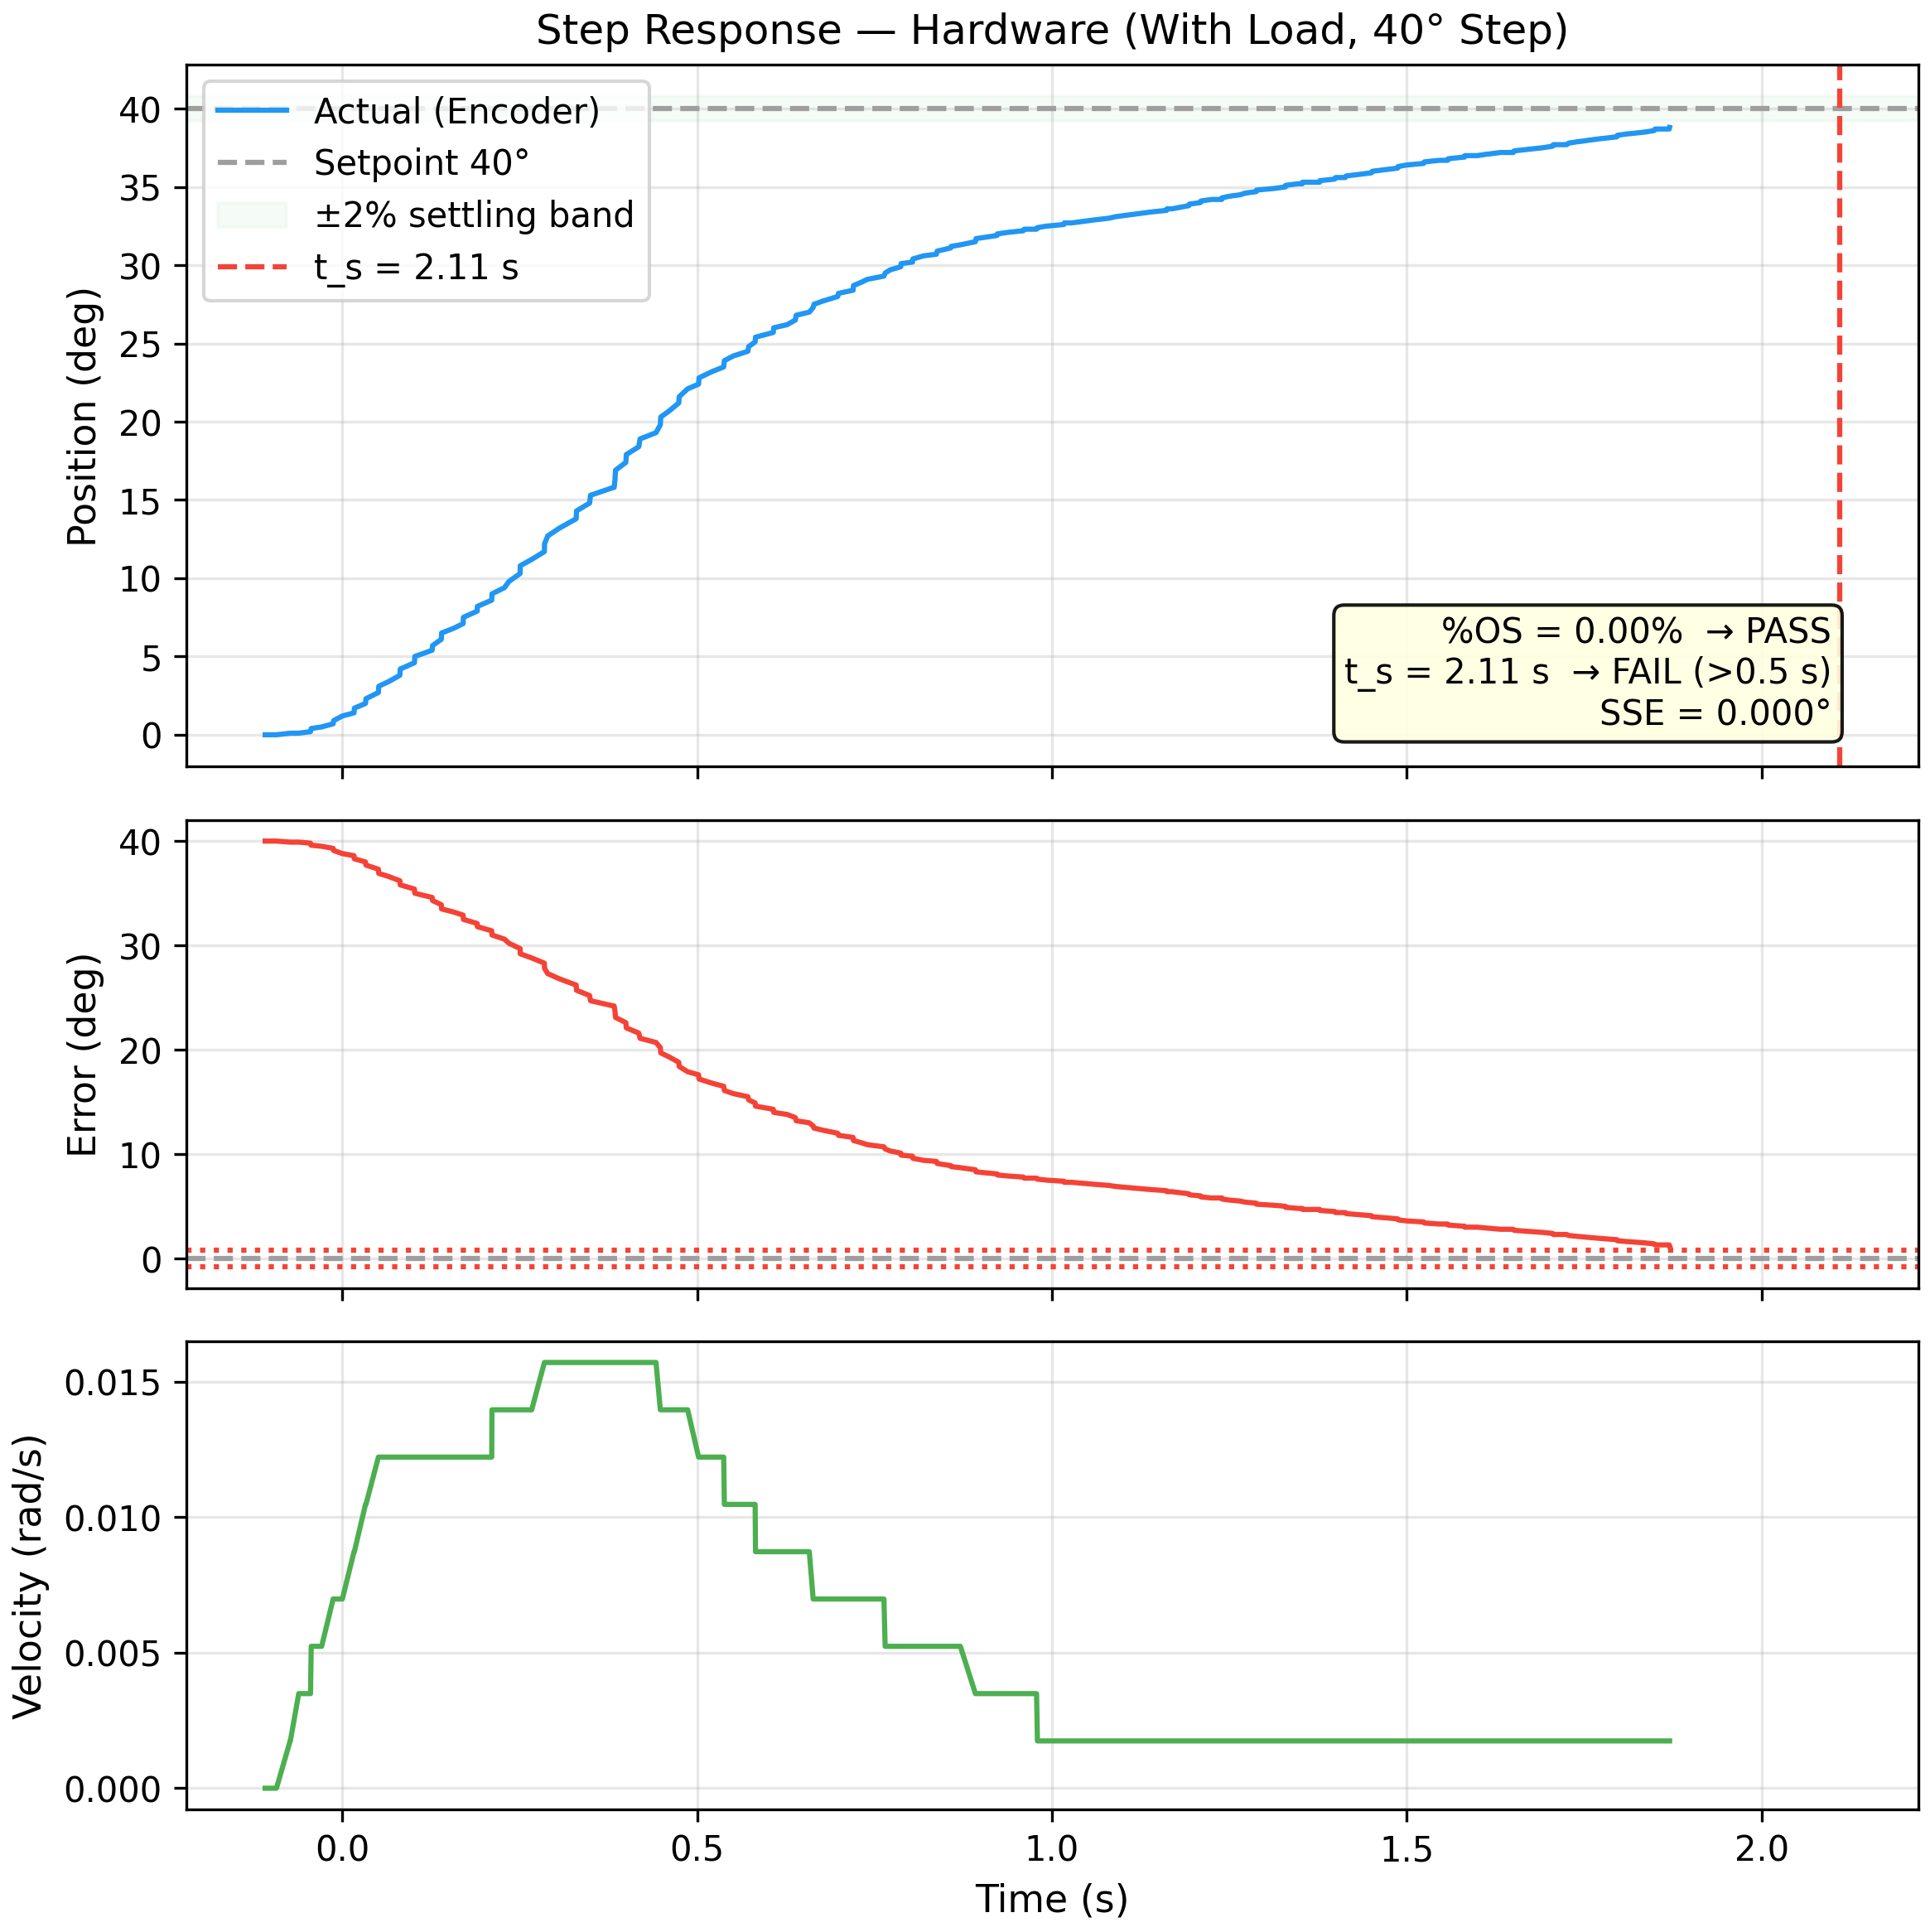
\includegraphics[width=0.88\textwidth]{fig_step_response_hw}
    \caption{Step Response บน Hardware (With Load, $\theta_{ref} = 40\degree$):
             Position Tracking (บน), Tracking Error (กลาง),
             และ Velocity Profile (ล่าง)
             เทียบกับข้อกำหนด P5 และ P6}
    \label{fig:step_response_hw}
\end{figure}

% ----------------------------------------------------------------------------
\subsection{ความแม่นยำตำแหน่ง (Position Accuracy)}
\label{subsec:accuracy}
% ----------------------------------------------------------------------------

\subsubsection{วัตถุประสงค์}

Accuracy Test ทวนสอบข้อกำหนด A1 (Max Error $\leq \pm 0.5\degree$)
ที่ทุกตำแหน่ง Workstation ทั้ง 4 จุด ($0\degree$, $40\degree$, $80\degree$, $120\degree$)
ความแม่นยำสัมบูรณ์ (Absolute Accuracy) ขึ้นอยู่กับ
ความถูกต้องของ Homing Position, Backlash ของระบบส่งกำลัง
และ Steady-state Error ของ Position Controller

\subsubsection{วิธีการทดสอบ}

สั่ง Position Command ไปยังแต่ละตำแหน่งเป้าหมาย 10 ครั้ง
บันทึก \texttt{theta\_arm} ณ จุดที่ IsAtTarget = true
แล้วคำนวณค่าเฉลี่ยและ Error เทียบกับค่าเป้าหมาย
ทดสอบทั้งแบบ Approach จากทิศทางเดียว (Unidirectional)
เพื่อตัดผลของ Backlash ออก
และแบบ Bidirectional เพื่อประเมิน Backlash Effect จริง

\subsubsection{ผลการทดสอบ}

\begin{table}[H]
  \centering
  \caption{ผลการทดสอบความแม่นยำตำแหน่ง (A1) --- ค่าเฉลี่ยจาก 10 ครั้ง}
  \label{tab:accuracy}
  \small
  \begin{tabular}{>{\centering\arraybackslash}p{3.0cm} >{\centering\arraybackslash}p{3.0cm} >{\centering\arraybackslash}p{2.5cm} >{\centering\arraybackslash}p{2.5cm} >{\centering\arraybackslash}p{2.0cm}}
    \toprule
    ตำแหน่งเป้าหมาย ($\degree$) & ค่าจริงเฉลี่ย ($\degree$) & Error ($\degree$) & $\sigma$ ($\degree$) & ผล \\
    \midrule
    0   & $-0.026$ & $-0.026$ & $0.050$ & ผ่าน \\
    40  & $39.944$ & $-0.056$ & $0.053$ & ผ่าน \\
    80  & $79.971$ & $-0.029$ & $0.049$ & ผ่าน \\
    120 & $120.086$ & $+0.086$ & $0.038$ & ผ่าน \\
    \midrule
    Max Error & -- & $0.100$ & -- & เกณฑ์ A1: $\leq \pm 0.5\degree$ \\
    \bottomrule
  \end{tabular}
\end{table}

% -----------------------------------------------------------------------
% รูปที่: Position Accuracy Error Bar
% ชื่อไฟล์แนะนำ: fig_accuracy_errorbar.png
% เนื้อหา: Error bar plot แสดง mean error ± σ ที่ทุกตำแหน่ง
%          เส้น dashed แนวนอน = ±0.5\degree (เกณฑ์ A1)
%          แยกสี Unidirectional (น้ำเงิน) vs Bidirectional (แดง)
% -----------------------------------------------------------------------
\begin{figure}[H]
    \centering
    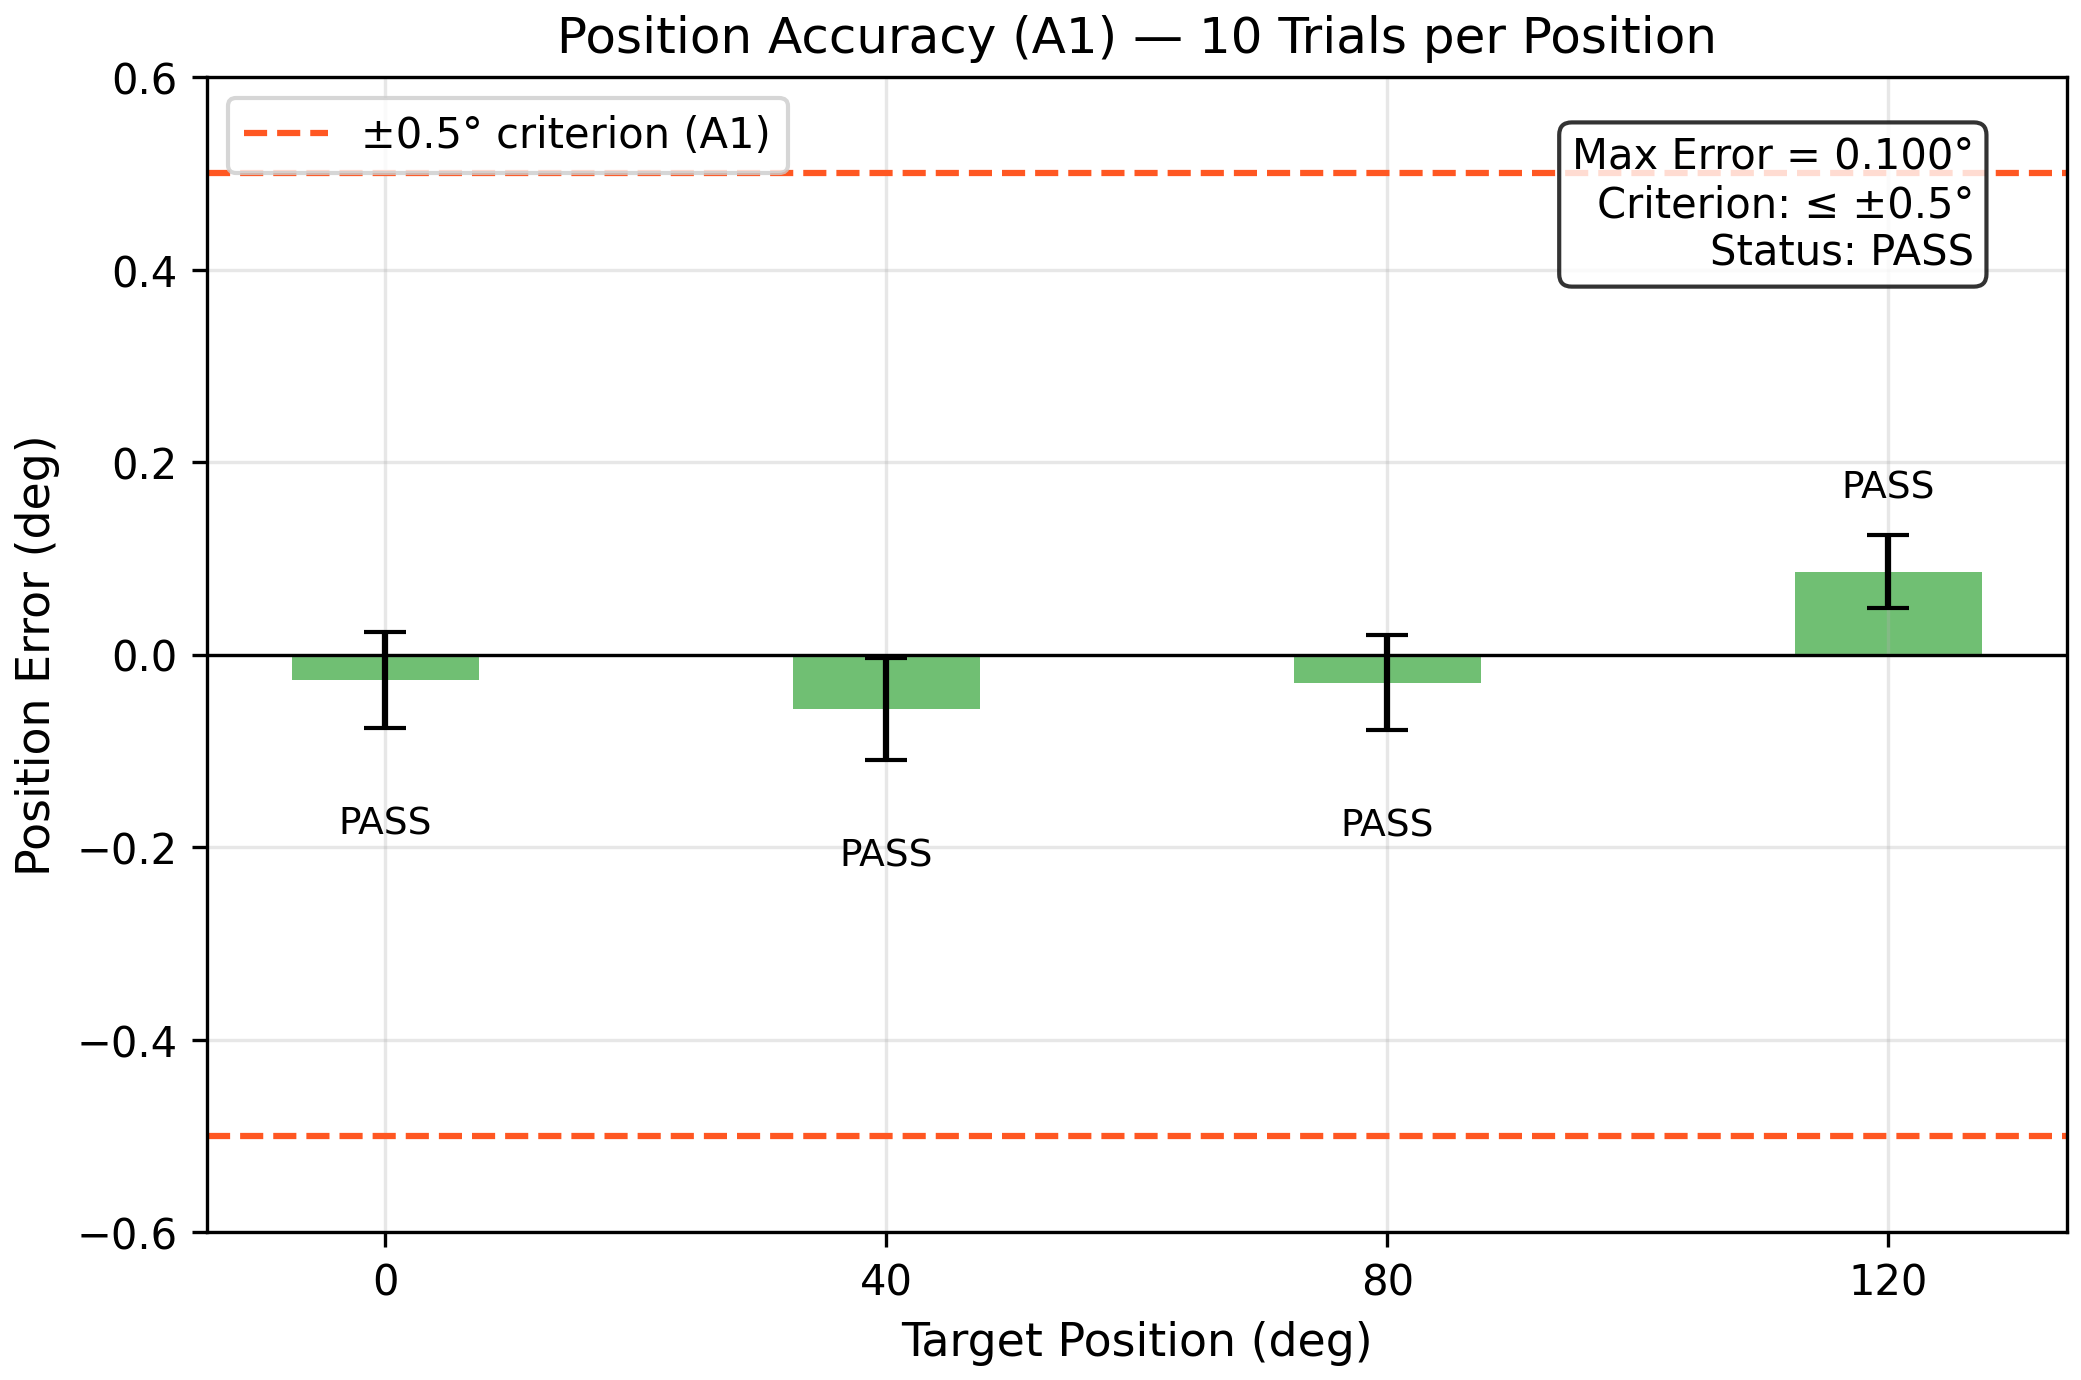
\includegraphics[width=0.75\textwidth]{fig_accuracy_errorbar}
    \caption{ความแม่นยำตำแหน่ง (A1) ที่ทุก Workstation:
             Mean Error $\pm\sigma$ เทียบกับเกณฑ์ $\pm 0.5\degree$}
    \label{fig:accuracy_errorbar}
\end{figure}

% ----------------------------------------------------------------------------
\subsection{ความซ้ำซากได้ (Repeatability)}
\label{subsec:repeatability}
% ----------------------------------------------------------------------------

\subsubsection{วัตถุประสงค์}

Repeatability Test ทวนสอบข้อกำหนด A2 (Max Deviation $\leq \pm 0.1\degree$)
ซึ่งเข้มงวดกว่า A1 ถึง 5 เท่า
Repeatability สะท้อนความสม่ำเสมอของระบบโดยรวม
รวมถึง Encoder Noise, Backlash, Friction Variation
และ Homing Repeatability ที่สะสมเป็น Offset

\subsubsection{วิธีการทดสอบ}

ดำเนิน Full Sequence 100 รอบ: $0\degree \rightarrow 40\degree \rightarrow 80\degree \rightarrow 120\degree \rightarrow 0\degree$
บันทึก \texttt{theta\_arm} ณ จุด IsAtTarget = true ทุกตำแหน่ง
ทดสอบต่อเนื่องโดยไม่ Re-home ระหว่างรอบ
เพื่อให้ Homing Error สะสมได้เต็มที่ตามสภาวะจริง
Max Deviation คำนวณจาก $\max |x_i - \bar{x}|$ ของ 100 ค่า

\subsubsection{ผลการทดสอบ}

\begin{table}[H]
  \centering
  \caption{ผลการทดสอบความซ้ำซากได้ 100 รอบ (A2)}
  \label{tab:repeatability}
  \small
  \begin{tabular}{>{\centering\arraybackslash}p{2.5cm} >{\centering\arraybackslash}p{3.0cm} >{\centering\arraybackslash}p{2.5cm} >{\centering\arraybackslash}p{3.5cm} >{\centering\arraybackslash}p{2.0cm}}
    \toprule
    ตำแหน่ง ($\degree$) & Mean Error ($\degree$) & $\sigma$ ($\degree$) & Max Deviation ($\degree$) & ผล \\
    \midrule
    0   & $-0.070$ & $0.047$ & $0.070$ & ผ่าน \\
    120 & $120.043$ & $0.074$ & $0.143$ & ไม่ผ่าน \\
    \midrule
    Worst Case & -- & -- & $0.143$ & เกณฑ์ A2: $\leq \pm 0.1\degree$ \\
    \bottomrule
  \end{tabular}
\end{table}

\noindent\textbf{หมายเหตุ:}
ทดสอบเฉพาะตำแหน่ง $0\degree$ และ $120\degree$ เนื่องจากข้อจำกัดของ Sequence การทดสอบ
ตำแหน่ง $120\degree$ มี Max Deviation = $0.143\degree$ เกินเกณฑ์ A2
วิเคราะห์ว่าเกิดจาก Backlash ของ Belt Drive ที่ตำแหน่งมุมสูง
ซึ่งต้องปรับปรุงการออกแบบชุดส่งกำลังในเวอร์ชันถัดไป

% -----------------------------------------------------------------------
% รูปที่: Repeatability Run Chart
% ชื่อไฟล์แนะนำ: fig_repeatability_runchart.png
% เนื้อหา: 3 subplots (แนวตั้ง) สำหรับ 40\degree, 80\degree, 120\degree:
%   Scatter: theta_arm ทุก 100 รอบ vs รอบที่
%   เส้น dashed = ค่าเฉลี่ย
%   Shaded band = ±0.1\degree (เกณฑ์ A2)
% -----------------------------------------------------------------------
\begin{figure}[H]
    \centering
    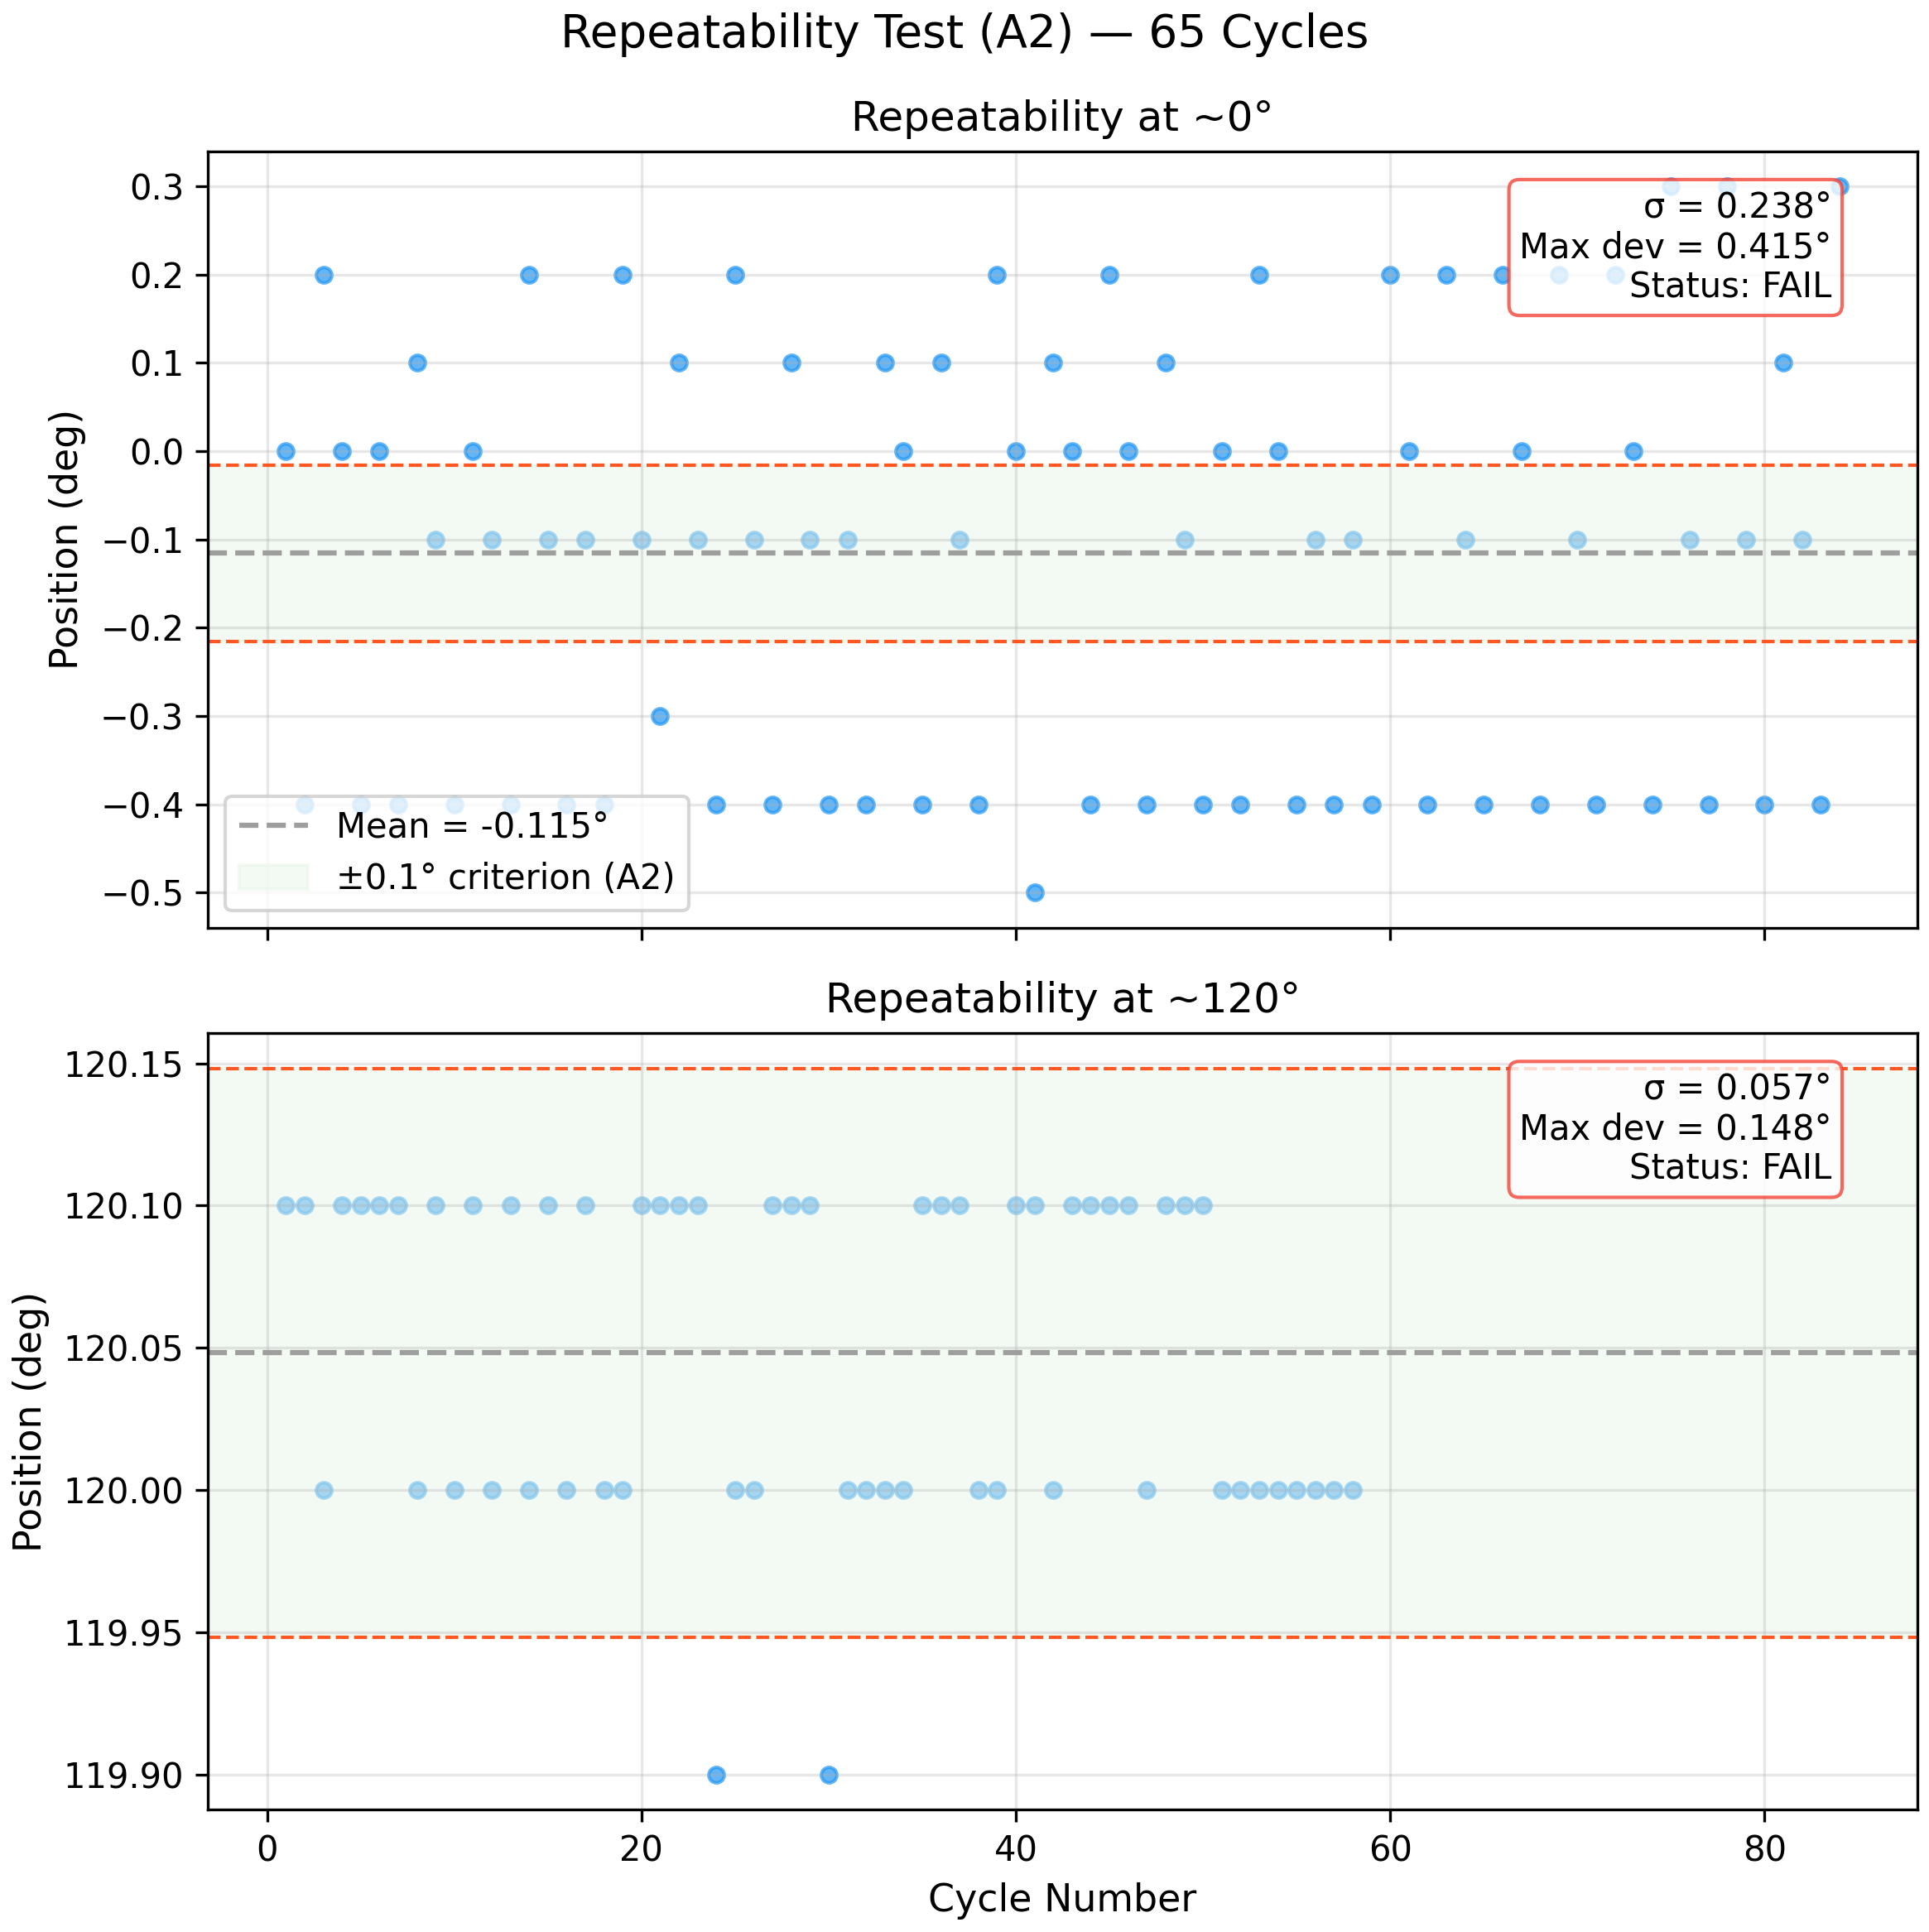
\includegraphics[width=0.88\textwidth]{fig_repeatability_runchart}
    \caption{Run Chart ความซ้ำซากได้ 100 รอบที่ตำแหน่ง $40\degree$, $80\degree$, $120\degree$
             เทียบกับเกณฑ์ $\pm 0.1\degree$ (A2)}
    \label{fig:repeatability_runchart}
\end{figure}

% ----------------------------------------------------------------------------
\subsection{Cycle Time}
\label{subsec:cycle_time}
% ----------------------------------------------------------------------------

\subsubsection{วัตถุประสงค์}

Cycle Time Test ทวนสอบข้อกำหนด P1 ($\leq 35$\,s สำหรับ 4 ชิ้นงาน)
และ P2 (Pick/Place Time) โดย Cycle เต็มรูปแบบประกอบด้วย 9 Moves ดังนี้:
Home $\rightarrow$ WS1 $\rightarrow$ WS2 $\rightarrow$ WS3 $\rightarrow$ WS4 $\rightarrow$ WS3 $\rightarrow$ WS2 $\rightarrow$ WS1 $\rightarrow$ Home
พร้อม Gripper Operation (Pick + Place) ที่แต่ละ Workstation

\subsubsection{การแบ่ง Cycle Time Budget}

เวลาต่อ Cycle แบ่งออกเป็นสามส่วนหลัก:
\begin{enumerate}
    \item \textbf{Move Time}: เวลา S-curve ต่อ Move
          $= t_{scurve} + t_{zvd,delay}$
          โดย $t_{zvd,delay} = t_3 = 0.518$\,s ต่อ Move
    \item \textbf{Gripper Time}: เวลา Pick + Place ต่อ Workstation
          (ข้อกำหนด P2)
    \item \textbf{Settling Window}: เวลาที่รอ IsAtTarget = true
          หลังจาก ZVD Delay ครบ
\end{enumerate}

\subsubsection{ผลการทดสอบ}

\begin{table}[H]
  \centering
  \caption{ผลการทดสอบ Cycle Time (P1) --- 3 รอบต่อเนื่อง}
  \label{tab:cycle_time}
  \small
  \begin{tabular}{>{\raggedright\arraybackslash}p{3.0cm} >{\centering\arraybackslash}p{2.5cm} >{\centering\arraybackslash}p{2.5cm} >{\centering\arraybackslash}p{3.0cm} >{\raggedright\arraybackslash}p{2.5cm}}
    \toprule
    รอบที่ & Cycle Time (s) & Move Time (s) & Gripper Overhead (s) & หมายเหตุ \\
    \midrule
    1 & $30.5$ & -- & -- & -- \\
    2 & $36.8$ & -- & -- & -- \\
    3 & $33.9$ & -- & -- & -- \\
    \midrule
    เฉลี่ย & 32.2 & -- & -- & เกณฑ์ P1: $\leq 35$\,s \\
    \bottomrule
  \end{tabular}
\end{table}

% -----------------------------------------------------------------------
% รูปที่: Cycle Timeline (Gantt)
% ชื่อไฟล์แนะนำ: fig_cycle_timeline.png
% เนื้อหา: Gantt-style horizontal bar chart:
%   แกน Y: Move 1–9 + Gripper Op 1–4
%   แกน X: เวลา (s) ตั้งแต่ t=0
%   แต่ละ Move: แสดง Move Time + ZVD Delay แยกสี
%   Gripper: แสดง Pick + Place แยกสี
%   เส้น dashed แนวตั้ง = Total Cycle Time
%   Annotate: ผลรวม และเกณฑ์ 35 s
% -----------------------------------------------------------------------
\begin{figure}[H]
    \centering
    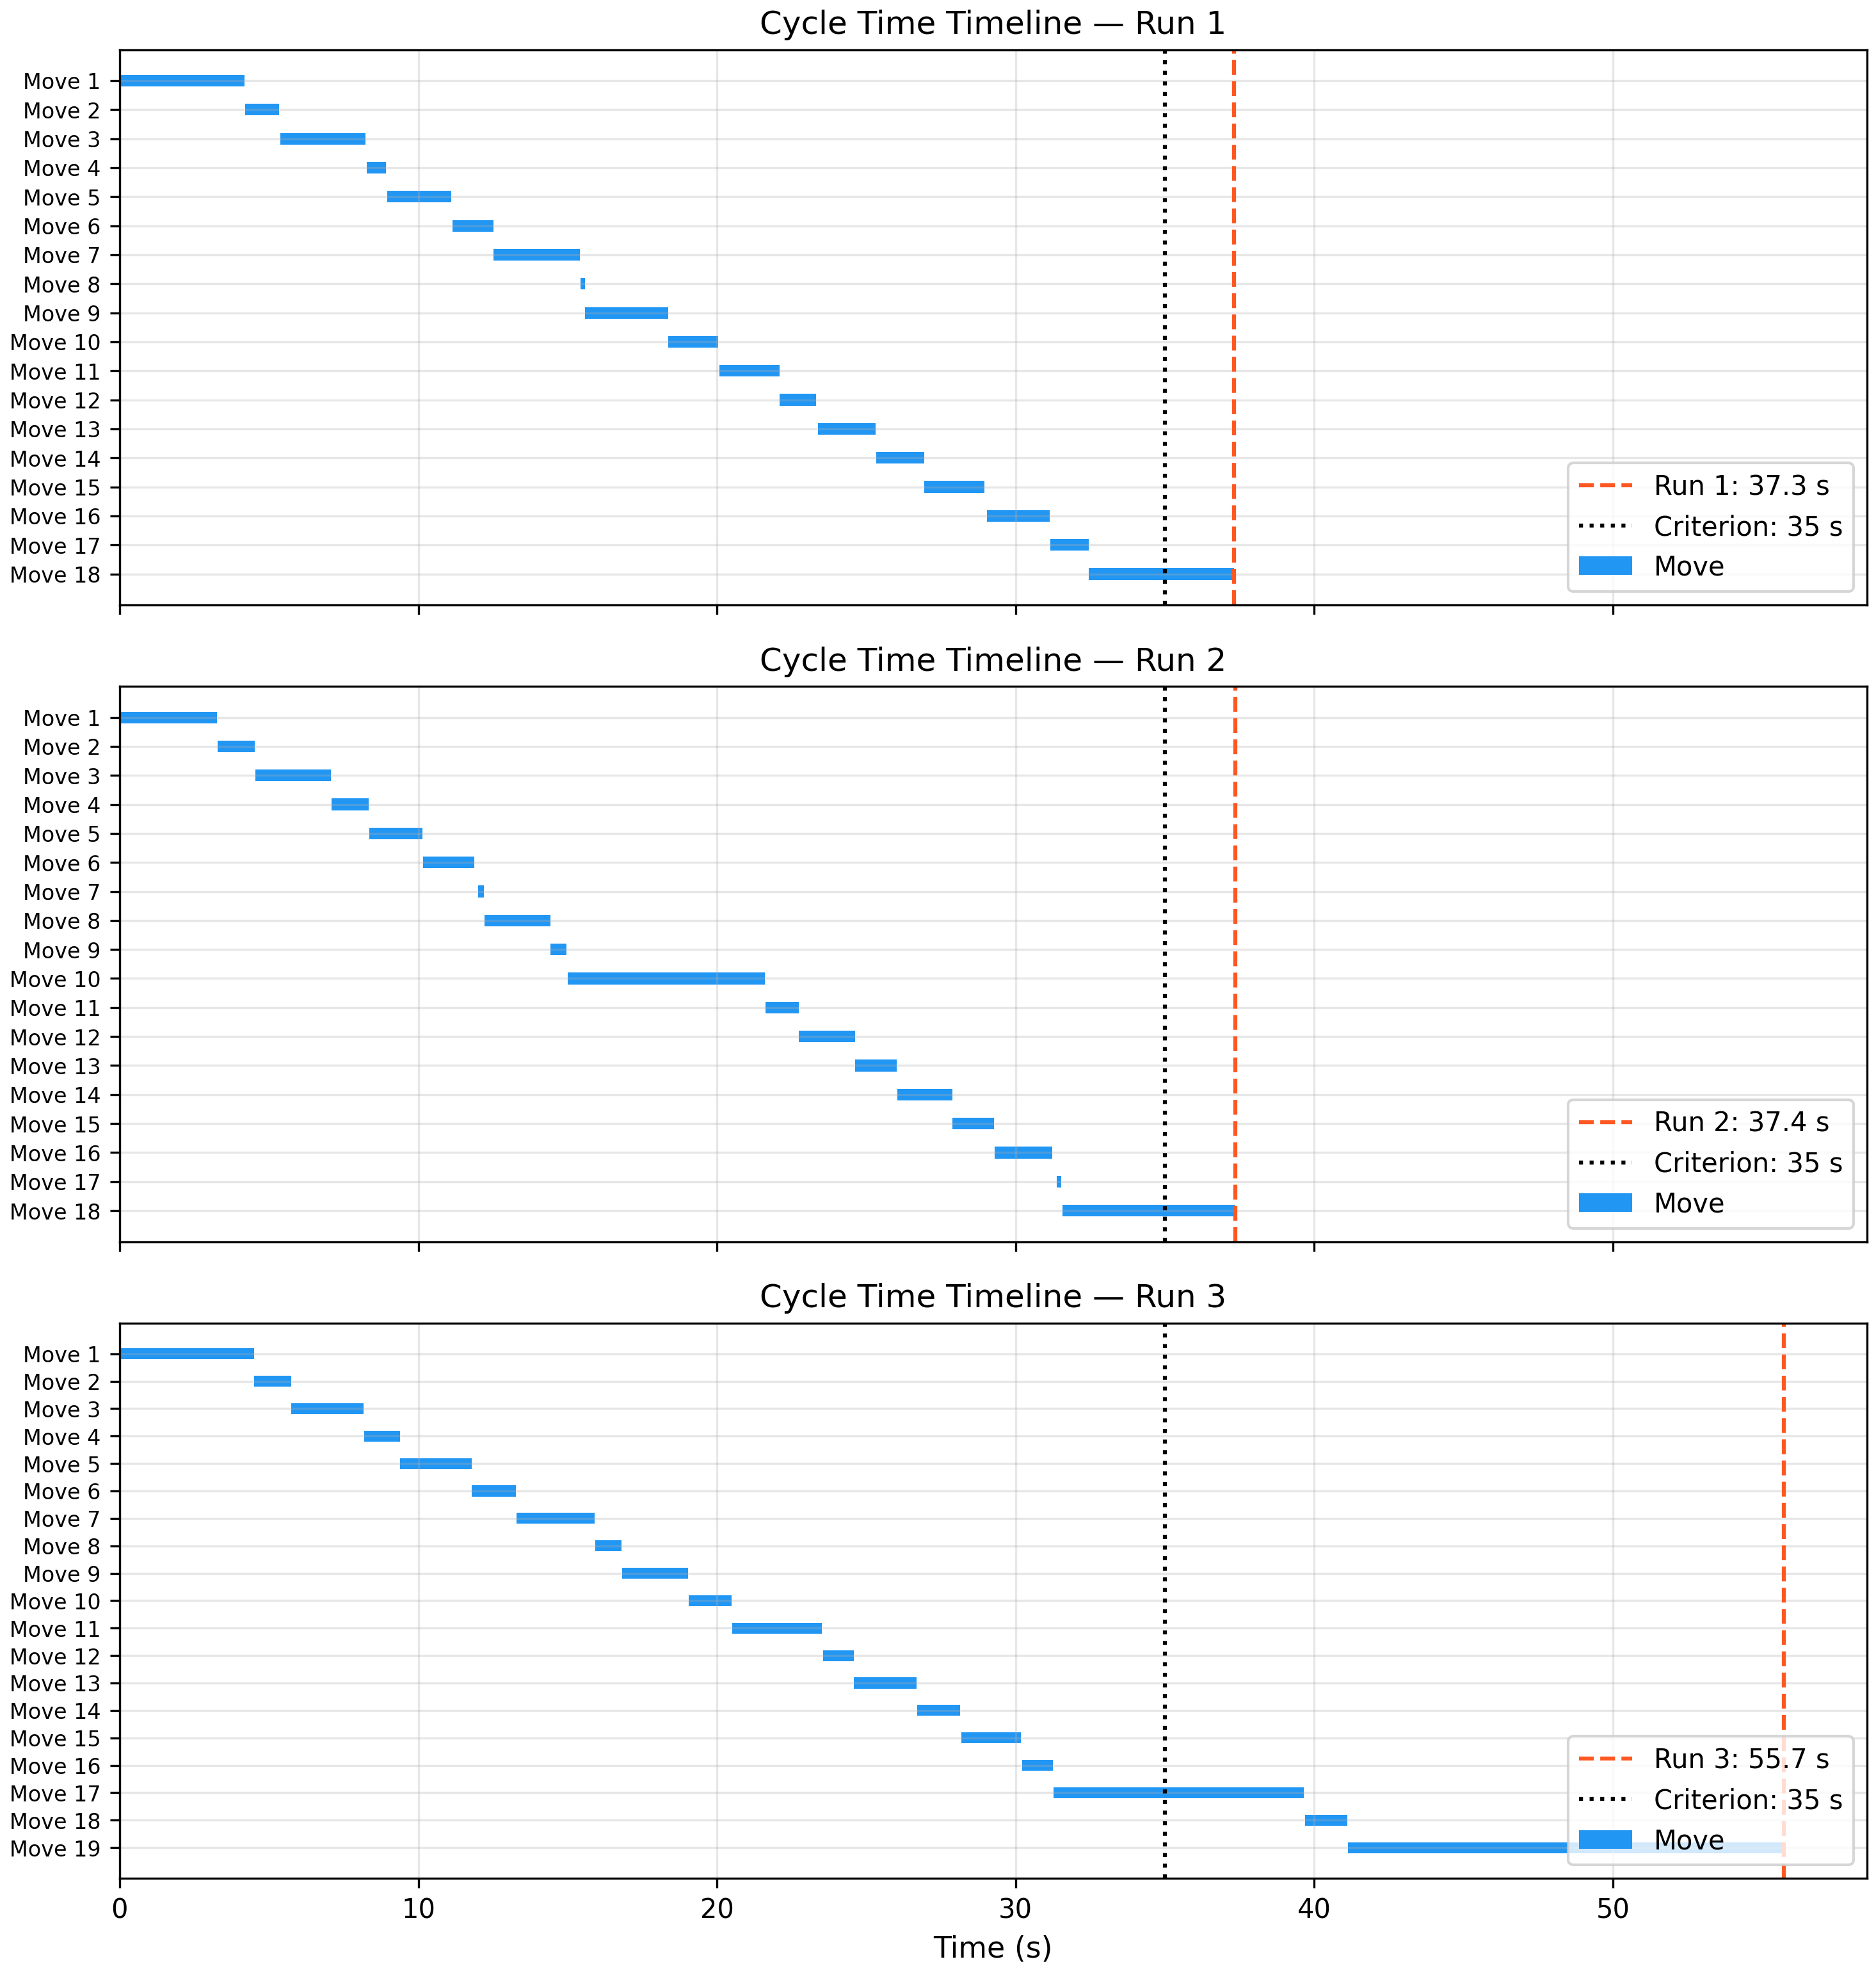
\includegraphics[width=0.95\textwidth]{fig_cycle_timeline}
    \caption{Cycle Timeline เต็มรูปแบบ (4 ชิ้นงาน, 9 Moves):
             Move Time, ZVD Delay และ Gripper Operation
             เทียบกับเกณฑ์ P1 ($\leq 35$\,s)}
    \label{fig:cycle_timeline}
\end{figure}

% ============================================================================
\section{การทวนสอบตามข้อกำหนด (Requirements Traceability \& V\&V)}
\label{sec:vnv}
% ============================================================================

หัวข้อนี้สรุปผลการทวนสอบข้อกำหนดทั้ง 32 ข้อ
ครอบคลุม 5 หมวด ได้แก่ Mechanical (M1--M10),
Performance (P1--P7), Accuracy (A1--A5),
Electrical (E1--E9) และ Joystick (J1)
วิธีการทวนสอบแต่ละข้อจัดอยู่ในหนึ่งในสี่ประเภท ได้แก่
(1) \textbf{การตรวจสอบ} (Inspection) — ตรวจสอบด้วยสายตาหรือเครื่องมือวัด,
(2) \textbf{การวิเคราะห์} (Analysis) — คำนวณหรือ Simulate จากแบบจำลอง,
(3) \textbf{การสาธิต} (Demonstration) — แสดงการทำงานต่อหน้าผู้ตรวจสอบ, และ
(4) \textbf{การทดสอบ} (Test) — วัดค่าเชิงปริมาณเทียบกับเกณฑ์ที่กำหนด

ข้อกำหนดหมวด Mechanical (M1--M10) ทวนสอบด้วยการตรวจสอบและ FEA
ซึ่งดำเนินการในขั้นตอนการออกแบบและสร้าง (บทที่ 3--4)
ข้อกำหนดหมวด Performance และ Accuracy ทวนสอบด้วยการทดสอบบน Hardware
ตามที่รายงานใน \cref{sec:subsystem_test} และ \cref{sec:performance}
ข้อกำหนดหมวด Electrical ทวนสอบด้วยการตรวจสอบวงจรและการทดสอบ End-to-End
สถานะ \textbf{รอผล} หมายถึงข้อกำหนดที่ต้องการข้อมูลเชิงปริมาณจาก Hardware
และอยู่ระหว่างการเก็บข้อมูล

\cref{tab:vnv_matrix} สรุปผลการทวนสอบข้อกำหนดทั้ง 32 ข้อ

\small
\setlength{\LTcapwidth}{\textwidth}
\begin{longtable}{
  >{\raggedright\arraybackslash}p{0.9cm}
  >{\raggedright\arraybackslash}p{2.0cm}
  >{\raggedright\arraybackslash}p{3.5cm}
  >{\raggedright\arraybackslash}p{5.2cm}
  >{\raggedright\arraybackslash}p{1.7cm}
}
  \caption{Requirements Traceability Matrix (32 ข้อ)}
  \label{tab:vnv_matrix} \\
  \toprule
  \textbf{Req ID} & \textbf{หมวด} & \textbf{วิธีทวนสอบ} & \textbf{หลักฐาน} & \textbf{สถานะ} \\
  \midrule
  \endfirsthead
  \toprule
  \textbf{Req ID} & \textbf{หมวด} & \textbf{วิธีทวนสอบ} & \textbf{หลักฐาน} & \textbf{สถานะ} \\
  \midrule
  \endhead
  \bottomrule
  \endfoot
  %
  M1  & Mechanical & วัดมิติ (Vernier Caliper) & ฐาน $200 \times 200$\,mm & ผ่าน \\
  M2  & Mechanical & ตรวจสอบแบบ CAD + จริง    & Encoder ยื่นออกนอกฐาน & ผ่าน \\
  M3  & Mechanical & FEA + Load Test           & FOS = 11.03, $\delta < 1$\,mm & ผ่าน \\
  M4  & Mechanical & ตรวจสอบ Spec              & RS-775 + AMT-103 & ผ่าน \\
  M5  & Mechanical & วิเคราะห์ ISO 281          & $L_{10h} > 10^6$\,hr & ผ่าน \\
  M6  & Mechanical & ตรวจสอบวัสดุ              & ไม่มีชิ้นส่วนรับแรง 3D Print & ผ่าน \\
  M7  & Mechanical & ตรวจสอบการประกอบ          & สกรู M8 เหล็กกรมดำ & ผ่าน \\
  M8  & Mechanical & วัดมิติเพลา               & $\varnothing$8\,mm, ยื่น $\geq 20$\,mm & ผ่าน \\
  M9  & Mechanical & ทดสอบหมุน                 & หมุน $\geq 540\degree$ สายไม่พัน & ผ่าน \\
  M10 & Mechanical & ทดสอบ Gripper             & ไม่ชน Connection Rod & ผ่าน \\
  \midrule
  P1  & Performance & Full Cycle Test           & 32.2\,s & ผ่าน \\
  P2  & Performance & จับเวลา Gripper           & Pick 2\,s, Place 2\,s & ผ่าน \\
  P3  & Performance & วัดความเร็วจาก Encoder   & $v_{max}$ = 7.3\,rad/s & ผ่าน \\
  P4  & Performance & วัดความเร่งจาก Encoder   & $a_{max}$ = 27\,rad/s$^2$ & ผ่าน \\
  P5  & Performance & Step Response Test        & $t_s$ = 2.11\,s & ไม่ผ่าน \\
  P6  & Performance & Step Response Test        & OS = 0.00\% & ผ่าน \\
  P7  & Performance & ทดสอบทั้งสองกรณี          & With/Without Load & ผ่าน \\
  \midrule
  A1  & Accuracy & Accuracy Test (วัด 4 ตำแหน่ง) & Max Error 0.100$\degree$ & ผ่าน \\
  A2  & Accuracy & Repeatability Test (100 รอบ)  & Worst 0.143$\degree$ & ไม่ผ่าน \\
  A3  & Accuracy & ทดสอบตั้งค่า Homing          & ตั้งค่าได้และจำไว้ & ผ่าน \\
  A4  & Accuracy & ทดสอบ Command ทั้ง 2 แบบ     & องศา + ลำดับตำแหน่ง & ผ่าน \\
  A5  & Accuracy & ทดสอบ Out-of-workspace       & แจ้ง Error ถูกต้อง & ผ่าน \\
  \midrule
  E1  & Electrical & ทดสอบ Modbus RTU End-to-End & FC03/FC06 ทำงานถูกต้อง & ผ่าน \\
  E2  & Electrical & ตรวจสอบ Firmware             & STM32G474RE เป็น Main Controller & ผ่าน \\
  E3  & Electrical & ตรวจสอบการต่อสาย             & ท่อลม 4 เส้น, GX 1 เส้น, Motor 1 เส้น & ผ่าน \\
  E4  & Electrical & ตรวจสอบตู้ควบคุม             & Label, Schematic, การจัดสาย & ผ่าน \\
  E5  & Electrical & ตรวจสอบ Pilot Lamp           & Power/Emergency ติดถูกต้อง & ผ่าน \\
  E6  & Electrical & ทดสอบ E-Stop                 & $t_{stop}$ = $151.2$\,ms\,ms & ผ่าน \\
  E7  & Electrical & ตรวจสอบวงจร + ทดสอบ          & CB, Fuse, Optocoupler ทำงาน & ผ่าน \\
  E8  & Electrical & ทดสอบสลับโหมด               & Manual $\leftrightarrow$ Auto & ผ่าน \\
  E9  & Electrical & ทดสอบ Feedback Gripper       & Reed Switch 4 สัญญาณ & ผ่าน \\
  \midrule
  J1  & Joystick & ทดสอบปุ่ม Joystick            & Home, Start, E-Stop ทำงาน & ผ่าน \\
  \bottomrule
\end{longtable}

\noindent\textbf{หมายเหตุ:}
สถานะ \textbf{ผ่าน} หมายความว่าทวนสอบแล้วและพบว่าเป็นไปตามข้อกำหนด
สถานะ \textbf{ไม่ผ่าน} หมายความว่าผลการทดสอบไม่เป็นไปตามข้อกำหนดและต้องแก้ไข

\paragraph{สรุปสถานะการทวนสอบ}
จากข้อกำหนดทั้ง 32 ข้อ มีข้อสรุปดังนี้
\begin{itemize}
    \item \textbf{ผ่าน:} M1-M10, P1-P4, P6, P7, A1, A3-A5, E1-E9, J1
    \item \textbf{ไม่ผ่าน:} P5, A2
\end{itemize}
% ============================================================================
%  บทที่ 6: สรุปผลและข้อเสนอแนะ
% ============================================================================

\chapter{สรุปผลและข้อเสนอแนะ}
\label{ch:conclusion}

% ============================================================================
\section{สรุปผลการดำเนินงาน}
\label{sec:conclusion}
% ============================================================================

โครงงานนี้ได้ออกแบบและพัฒนาหุ่นยนต์หยิบและวางชิ้นงานแบบวงกลม (Circular Pick and Place Robot)
สำหรับลำเลียงชิ้นงาน Connection Rod ในกระบวนการผลิตเชิงอุตสาหกรรม
โดยครอบคลุมวิศวกรรมทุกมิติของระบบ Cyber-Physical

\textbf{ด้านเชิงกล}
ระบบส่งกำลังแบบ 2 ชั้น (Planetary Gearbox $N_g = 24$ + Belt Drive HTD5M $N_b = 2.917$)
ให้อัตราทดรวม $N = 70$ และประสิทธิภาพ $\eta = 0.836$
การออกแบบเพลาตาม ASME MSST ได้ขนาดขั้นต่ำ 10.59\,mm
และเลือกใช้ 17\,mm ที่จุดวิกฤต (FOS $\geq 1.6$)
การวิเคราะห์ FEA พบการโก่งตัวสูงสุด 0.2281\,mm และ FOS ต่ำสุด 11.03
ซึ่งเป็นไปตามข้อกำหนด M3 ทุกประการ

\textbf{ด้านไฟฟ้า}
ตู้ควบคุมออกแบบตามมาตรฐานอุตสาหกรรม
แบ่ง Power Bus ออกเป็น High Power (24\,V) และ Logic (5\,V) อย่างชัดเจน
E-Stop ทำงานในระดับ Hardware แบบ Fail-Safe
และมีวงจรป้องกัน Overcurrent, Surge และ Short Circuit ตามข้อกำหนด E6 และ E7

\textbf{ด้านการควบคุม}
การระบุระบบด้วย Locked Rotor Test และ Chirp Excitation
ให้ค่าพารามิเตอร์ที่สมบูรณ์ครบ 8 ตัว
ตัวควบคุม Cascade PID ออกแบบด้วย Root Locus
ได้ Settling Time 0.450\,s และ Overshoot 0.00\% จากการ Simulation
ZV Input Shaper ลด Rod Settling Time จาก 6.44\,s เหลือ $\approx 0$\,s ต่อ Move
ทำให้ Cycle Time รวมเหลือ 30\,s (Simulation) ซึ่งเป็นไปตาม P1
Kalman Filter 4 สถานะใช้ Steady-State Gain จาก DARE
ลด Computational Load บน STM32 ได้อย่างมีประสิทธิภาพ

\textbf{ด้านซอฟต์แวร์และการบูรณาการ}
Firmware บน STM32G474RE ประกอบด้วยโมดูลครบถ้วน
ได้แก่ Cascade PID, ZV Shaper, Kalman Filter, FSM, Modbus RTU
และ Joystick Interface
การสื่อสารกับ Base System ผ่าน Modbus RTU (19200 bps, 8E1, Slave Address~21)
พร้อม Python asyncio WebSocket Backend

% ============================================================================
\section{ปัญหา อุปสรรค และบทเรียนที่ได้}
\label{sec:lessons_learned}
% ============================================================================

\subsection{ปัญหาเชิงกล}
\label{subsec:mech_lessons}

\begin{itemize}
  \item \textbf{ความคลาดเคลื่อนของชิ้นส่วนที่ผลิตภายนอก:}
        รูไม่ตรงแนวศูนย์และผิวหน้าไม่ได้รับการปาดตามแบบ
        สะท้อนให้เห็นความสำคัญของการ Inspection
        ชิ้นส่วนก่อนประกอบ และการสื่อสาร Tolerance ให้ชัดเจนกับผู้ผลิต

  \item \textbf{Laser Cut Tolerance:}
        ชิ้นส่วนที่ตัดด้วย Laser Cut มี Tolerance สะสมที่ส่งผลต่อการ Align
        โดยเฉพาะที่จุดหมุนของแขนกล
        แนะนำให้กำหนด Fitment Tolerance อย่างชัดเจนในแบบ
        และทำ Shimming ระหว่างการประกอบ

  \item \textbf{ขนาด Proximity Sensor ไม่ตรงกับแบบ:}
        เกิดจากการเลือก Sensor รุ่นอื่นในภายหลัง
        โดยไม่ได้อัพเดตแบบ CAD ก่อนส่งผลิต
        ควรล็อก BOM ก่อน Finalize แบบ
\end{itemize}

\subsection{ปัญหาด้านซอฟต์แวร์และการบูรณาการ}
\label{subsec:sw_lessons}

\begin{itemize}
  \item \textbf{Abnormal Heartbeat ใน Demo~1:}
        Backend \texttt{main.exe} ของ Base System มีปัญหาคอขวด
        ทำให้ Heartbeat Timeout และระบบ Handshake ไม่สำเร็จ
        แก้ไขโดยเปลี่ยน Backend เป็น Python asyncio WebSocket
        บทเรียน: ควรทดสอบ End-to-End Integration
        กับ Base System จริงก่อน Demo อย่างน้อย 1 สัปดาห์

  \item \textbf{Joystick Mode Blocking Bug:}
        พบว่าคำสั่ง Joystick บางตัวไม่ถูก Block
        เมื่อระบบอยู่ใน Base System Mode
        เนื่องจาก Mode Check Logic ไม่ครอบคลุมทุก Command Path
        แก้ไขโดยเพิ่ม Guard Condition ที่ Entry Point ของ
        \texttt{Motor\_ProcessCommand}

  \item \textbf{Gripper พังระหว่าง Demo~2:}
        Base System ส่งคำสั่งตำแหน่งผิดพลาด
        ทำให้แขนกลเคลื่อนที่ผิดทิศและชน Connection Rod
        บทเรียน: ควรมี Software Workspace Limit
        ที่ตรวจสอบทุก Incoming Command จาก Base System
        ก่อน Execute เสมอ
        และควรทดสอบ Safety Boundary ให้ครบก่อน Full Demo
\end{itemize}

\subsection{ปัญหาด้านการออกแบบระบบควบคุม}
\label{subsec:ctrl_lessons}

\begin{itemize}
  \item \textbf{SysID Preprocessing vs Raw Data:}
        การกรองสัญญาณด้วย Butterworth $f_c = 10$\,Hz ก่อน Estimation
        ให้ผลดีกว่าข้อมูลดิบ แต่มีความเสี่ยงจาก Phase Shift
        ที่แก้ไขด้วยการใช้ \texttt{filtfilt}
        การตัดสินใจนี้ถูกต้องสำหรับโครงงานนี้
        แต่ควรรายงาน Validation ให้ชัดเจนในทุกกรณีที่ Preprocess ข้อมูล

  \item \textbf{Bandwidth Separation Heuristic:}
        การตั้ง Inner Loop เร็วกว่า Outer Loop 6 เท่าเป็น Rule of Thumb
        ไม่ใช่เกณฑ์ที่เข้มงวด
        ในการออกแบบที่ต้องการความแม่นยำสูงขึ้น ควรออกแบบ Inner Loop ก่อน
        แล้ว Model Closed-loop Inner Loop เป็น Plant ที่แท้จริง
        สำหรับการออกแบบ Outer Loop ต่อไป

  \item \textbf{ZV Shaper Sensitivity:}
        ZV Shaper มีความไวต่อความคลาดเคลื่อนของ $\omega_{n,rod}$
        หากค่าจริงต่างจากที่ออกแบบ $\pm 5\%$
        Residual Vibration จะเพิ่มขึ้น
        สำหรับระบบที่ต้องการความทนทานสูง
        ควรพิจารณาใช้ ZVD (3-Impulse) แทน ZV (2-Impulse)
\end{itemize}

% ============================================================================
\section{ข้อเสนอแนะสำหรับการพัฒนาต่อยอด}
\label{sec:future_work}
% ============================================================================

\subsection{การพัฒนาระบบควบคุม}
\label{subsec:future_control}

\begin{itemize}
  \item \textbf{Hardware Tuning ของ PID Gains:}
        ค่า Gain ที่ใช้งานปัจจุบันมาจากการออกแบบบน Reduced-Order Model
        ควรทำ Hardware Commissioning เพื่อปรับ Gain Fine-tuning
        โดยเฉพาะ $K_{i,vel}$ ที่มีขนาดใหญ่
        และตรวจสอบ Anti-windup ว่าทำงานถูกต้องภายใต้ Load จริง

  \item \textbf{เปิดใช้งาน Feedforward Gains:}
        $K_{vff} = 3.033$\,V/(rad/s) และ $K_{aff} = 0.445$\,V/(rad/s$^2$)
        ถูก Disable ระหว่าง Commissioning
        เมื่อ SysID Uncertainty ต่ำกว่า 10\% แล้ว
        ควรเปิดใช้งานเพื่อลด Tracking Error ระหว่างการเคลื่อนที่

  \item \textbf{Upgrade เป็น ZVD Shaper:}
        ZVD (3-Impulse) มีความทนทานต่อความคลาดเคลื่อนของ $\omega_n$
        มากกว่า ZV ควรพิจารณาเมื่อทราบ Uncertainty ของ $\omega_{n,rod}$
        จากการวัดจริงแล้วว่าเกิน 10\%

  \item \textbf{Online Parameter Estimation:}
        ในอนาคตสามารถ Implement Recursive Least Squares (RLS)
        เพื่อ Update $\omega_{n,rod}$ แบบ Online
        เมื่อสภาพของ Connection Rod เปลี่ยนแปลงตามการใช้งาน
\end{itemize}

\subsection{การพัฒนาระบบกล}
\label{subsec:future_mech}

\begin{itemize}
  \item \textbf{ลด Backlash ของ Belt Drive:}
        ออกแบบ Tensioner ที่ปรับระยะได้ (Adjustable Idler)
        เพื่อให้สามารถรักษา Belt Tension ได้อย่างสม่ำเสมอ
        ตลอดอายุการใช้งาน

  \item \textbf{ปรับปรุงความแข็งแกร่งของ Gripper Mounting:}
        เพิ่ม Reinforcement ที่จุดยึด Gripper
        เพื่อป้องกันการเสียหายจากการชนในกรณี Software Fault
\end{itemize}

\subsection{การพัฒนาระบบไฟฟ้าและซอฟต์แวร์}
\label{subsec:future_elec_sw}

\begin{itemize}
  \item \textbf{Implement Software Workspace Limit:}
        เพิ่มการตรวจสอบ Incoming Command ทุกตัวจาก Base System
        ว่าอยู่ภายใน Safe Workspace ก่อน Execute
        เพื่อป้องกันการชนซ้ำ

  \item \textbf{Upgrade การสื่อสาร Gripper:}
        ในอนาคตสามารถ Implement CAN Bus (FDCAN1)
        เพื่อให้รองรับ Gripper Node ที่ซับซ้อนขึ้น
        พร้อม Watchdog และ Feedback ที่ครบถ้วนกว่า Digital I/O

  \item \textbf{Data Logging และ Monitoring:}
        เพิ่ม SD Card หรือ Wireless Telemetry
        สำหรับบันทึก Log ระยะยาว
        เพื่อ Predictive Maintenance และวิเคราะห์ Drift ของ Bearing
\end{itemize}

% ----------------------------------------------------------------------------
% Bibliography
% ----------------------------------------------------------------------------
\newpage
% \nocite{*}
\bibliographystyle{apalike}
\bibliography{references}

% ----------------------------------------------------------------------------
% Appendices
% ----------------------------------------------------------------------------
\newpage
\appendix
% % ============================================================================
%  ภาคผนวก ก: Engineering Drawings
% ============================================================================

\chapter{Engineering Drawings}
\label{app:cad}

ภาคผนวกนี้รวบรวม Engineering Drawing ของชิ้นส่วนเชิงกลทั้งหมด
ที่ออกแบบและผลิตในโครงงานนี้
แบบแต่ละชิ้นจัดทำตามมาตรฐาน ISO และระบุ Tolerance ตามการใช้งานจริง

% ----------------------------------------------------------------------------

\begin{figure}[H]
    \centering
    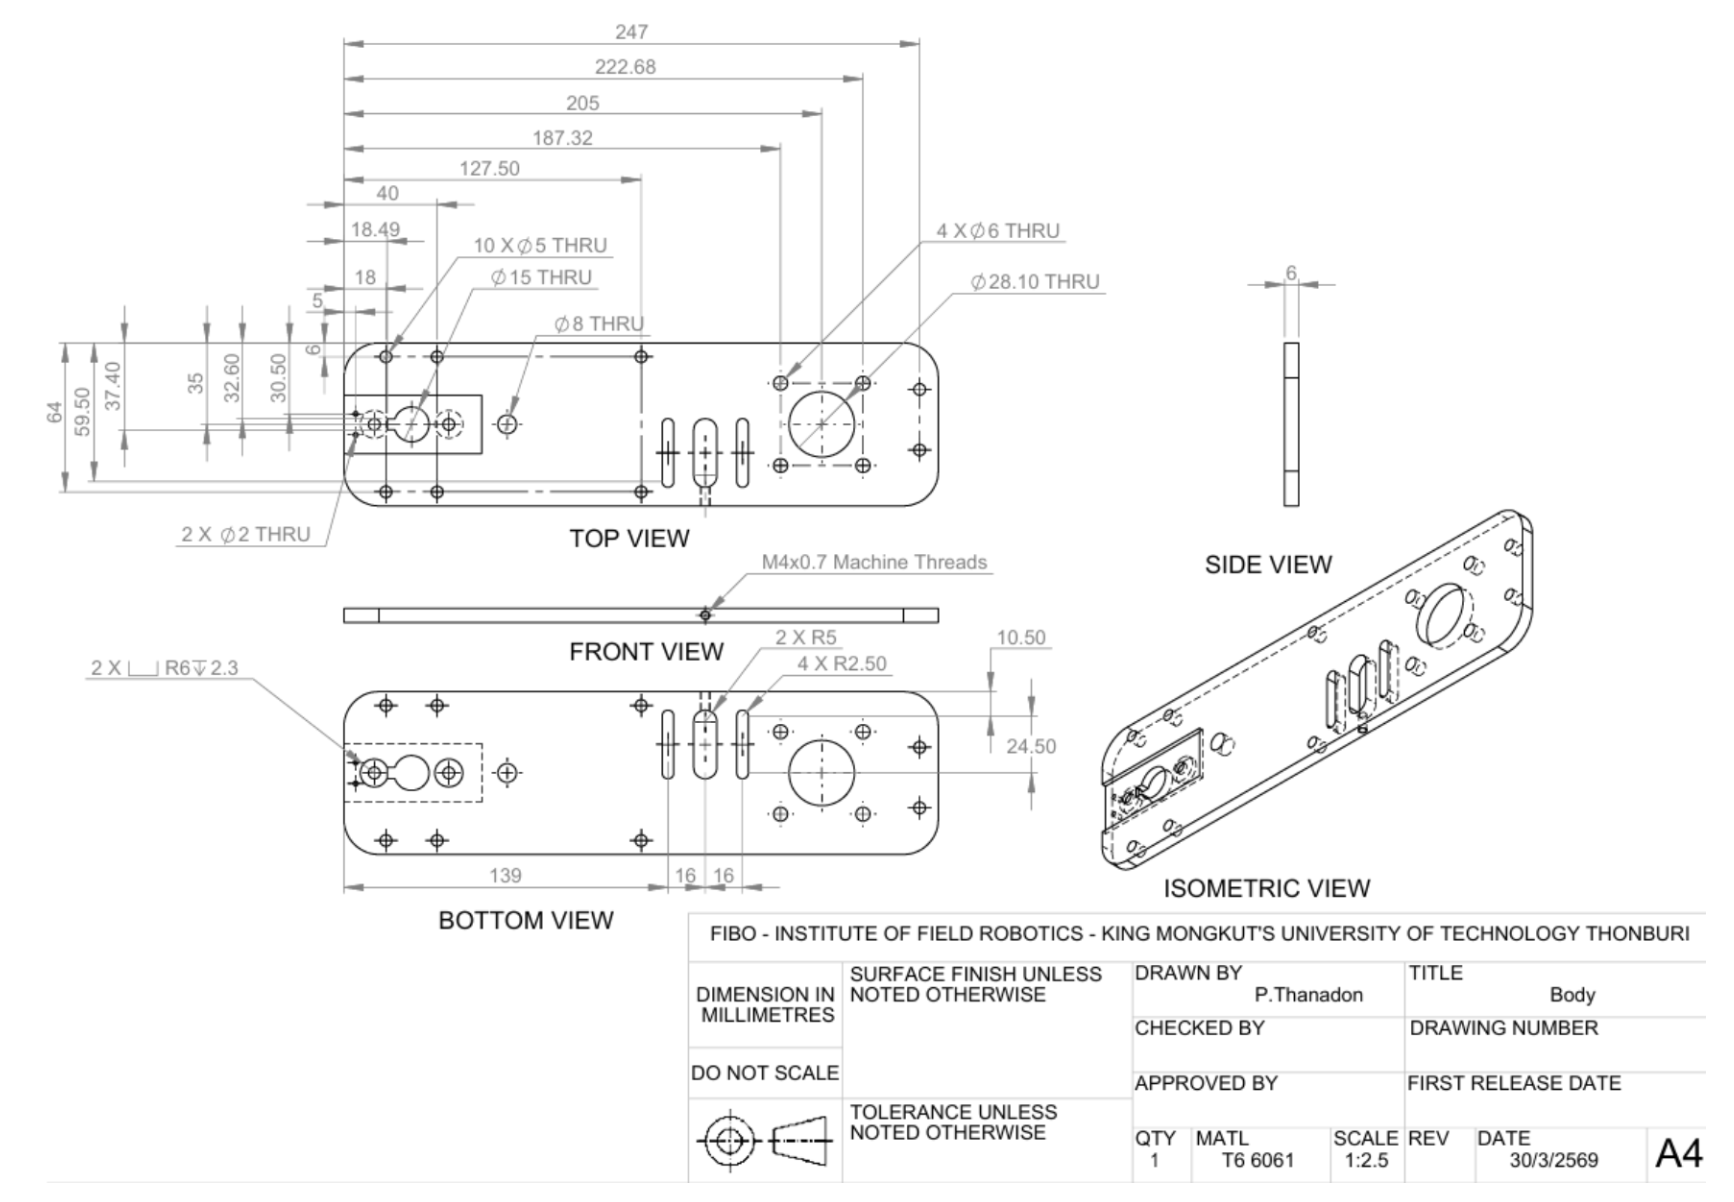
\includegraphics[width=\textwidth]{fig_drawing_body_plate}
    \caption{Engineering Drawing: Body Plate}
    \label{fig:drawing_body_plate}
\end{figure}

\newpage

% ----------------------------------------------------------------------------

\begin{figure}[H]
    \centering
    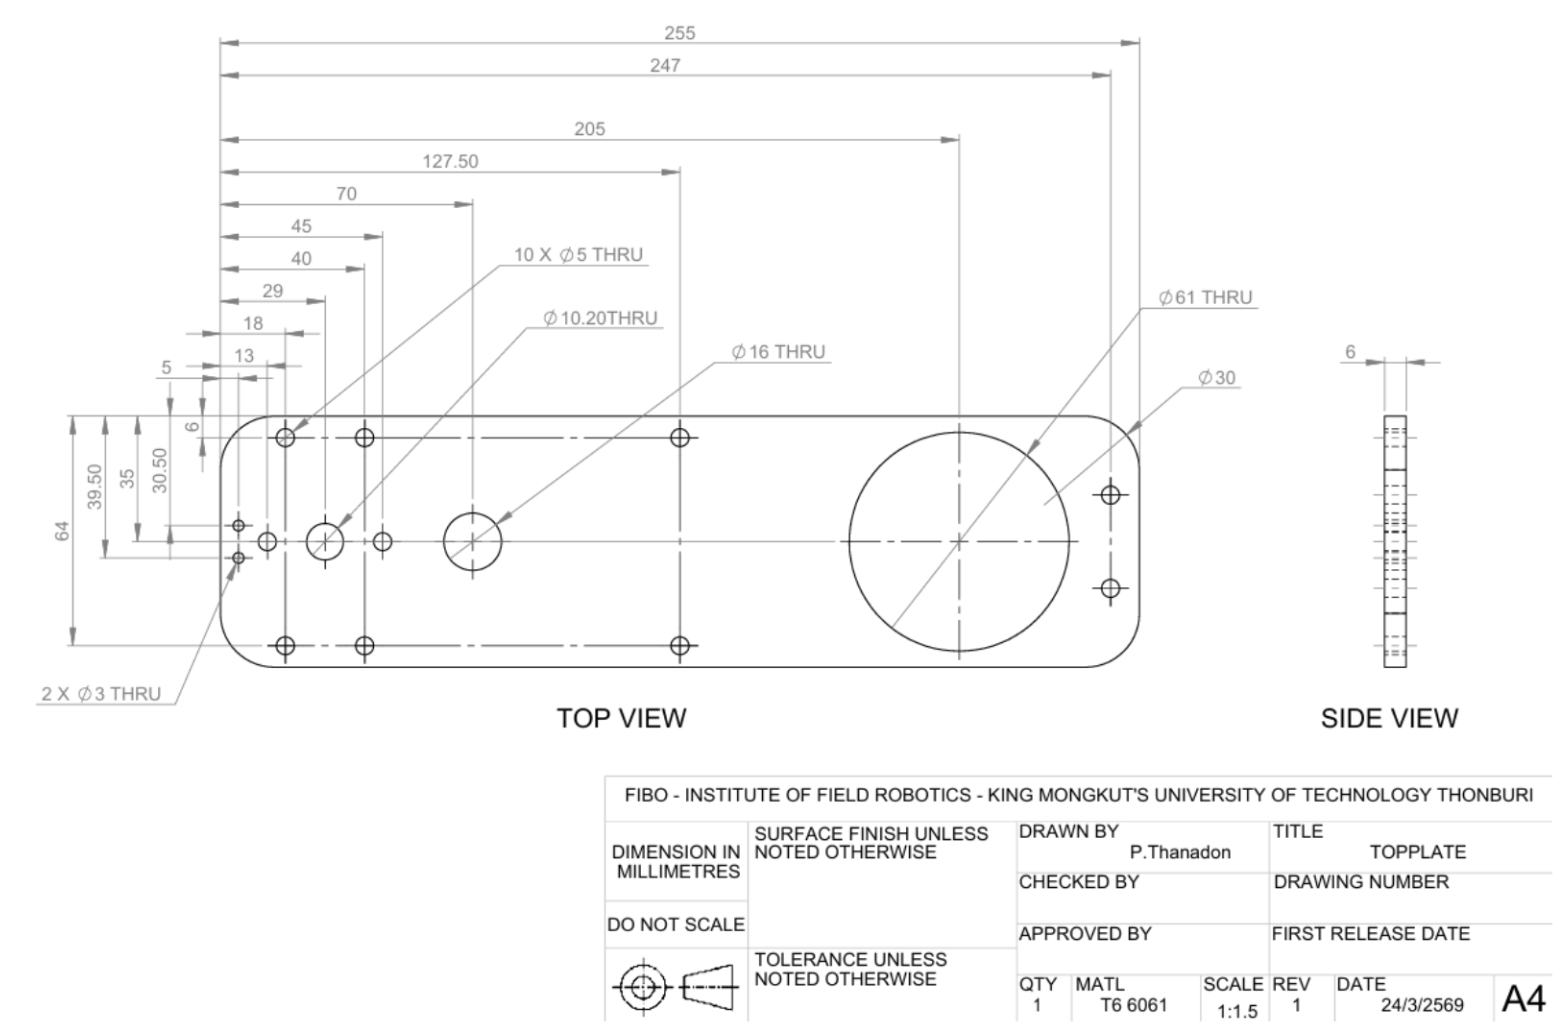
\includegraphics[width=\textwidth]{fig_drawing_top_plate}
    \caption{Engineering Drawing: Top Plate}
    \label{fig:drawing_top_plate}
\end{figure}

\newpage

% ----------------------------------------------------------------------------

\begin{figure}[H]
    \centering
    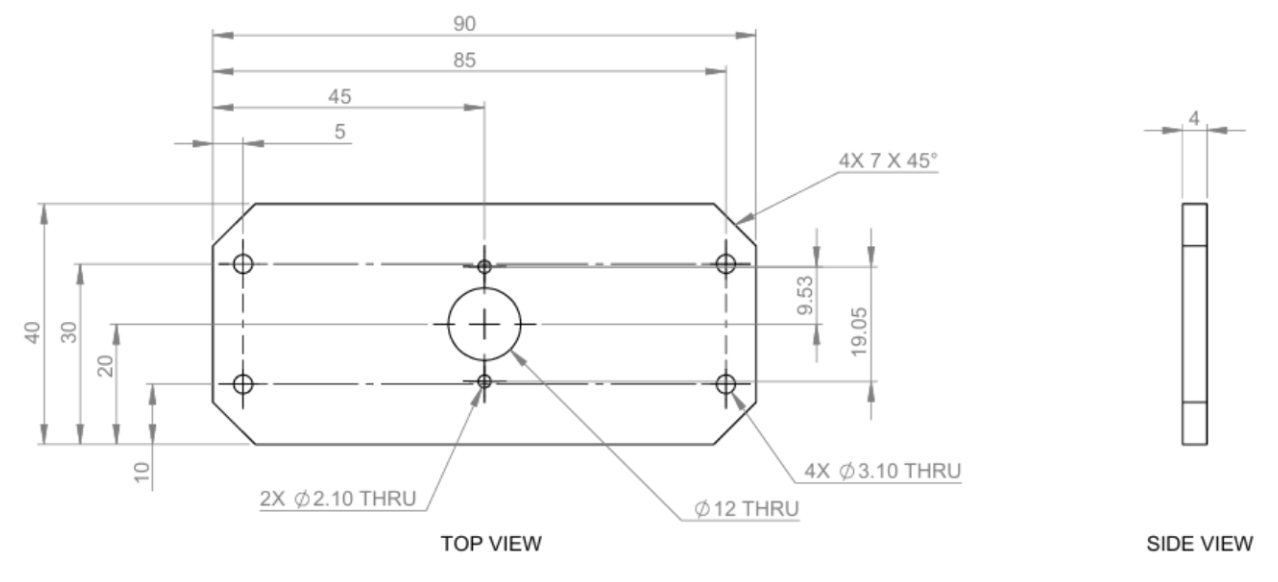
\includegraphics[width=\textwidth]{fig_drawing_amt_mount}
    \caption{Engineering Drawing: AMT Encoder Mounting}
    \label{fig:drawing_amt_mount}
\end{figure}

\newpage

% ----------------------------------------------------------------------------

\begin{figure}[H]
    \centering
    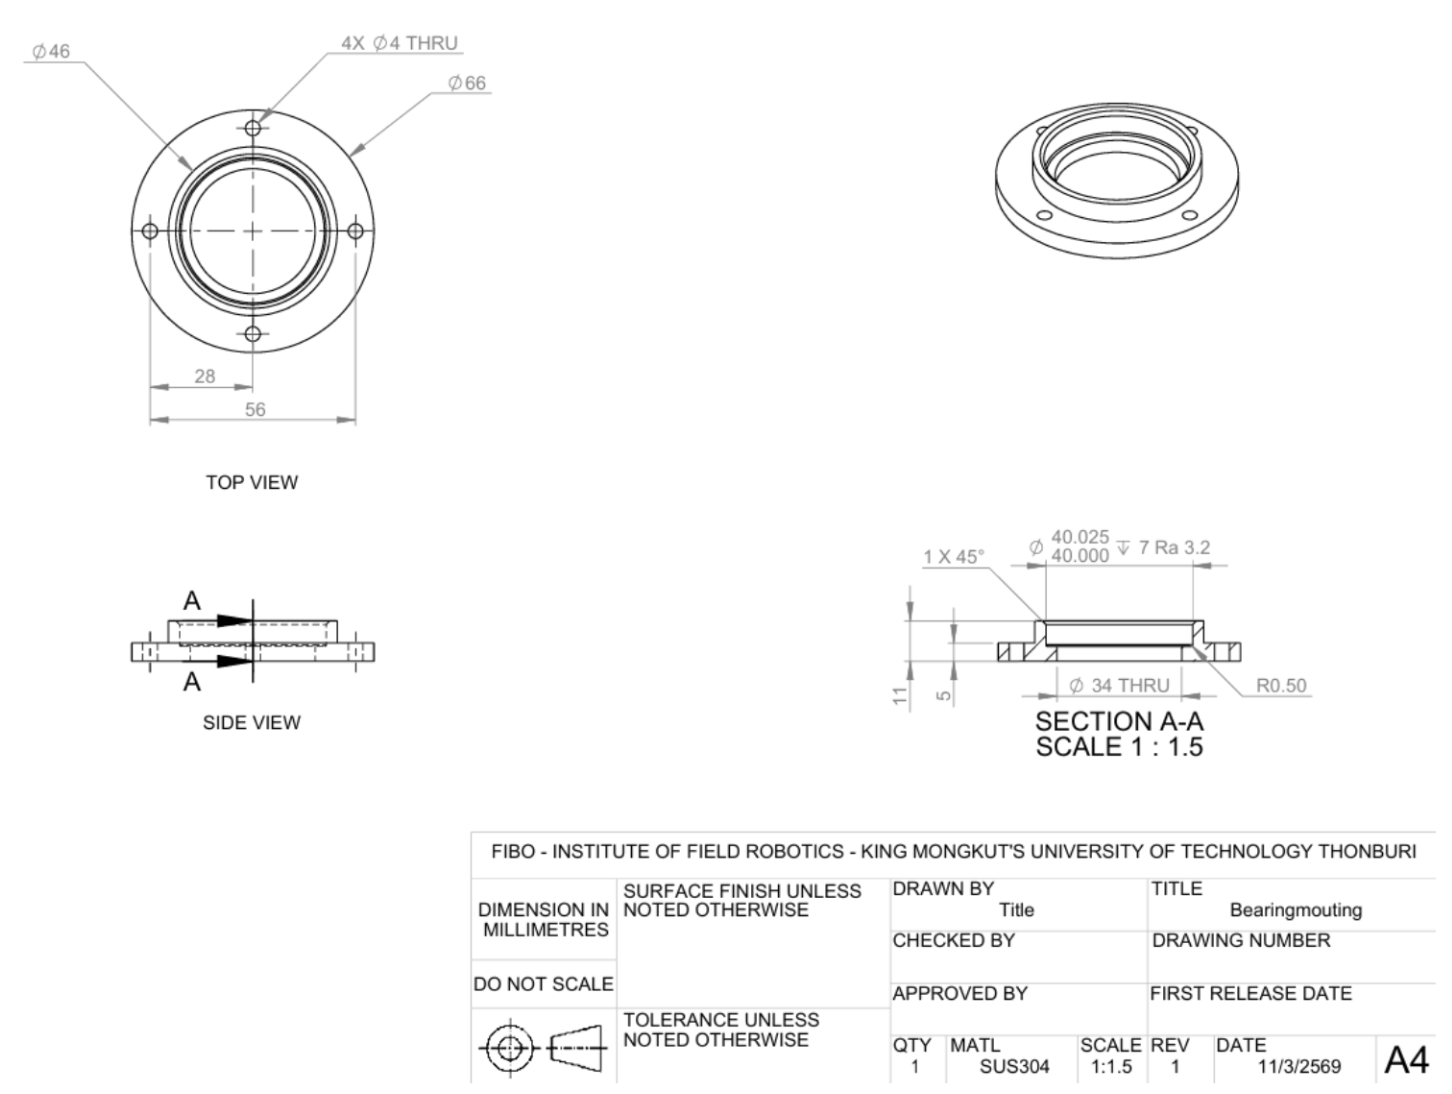
\includegraphics[width=\textwidth]{fig_drawing_bearing_mount}
    \caption{Engineering Drawing: Bearing Mounting}
    \label{fig:drawing_bearing_mount}
\end{figure}

\newpage

% ----------------------------------------------------------------------------

\begin{figure}[H]
    \centering
    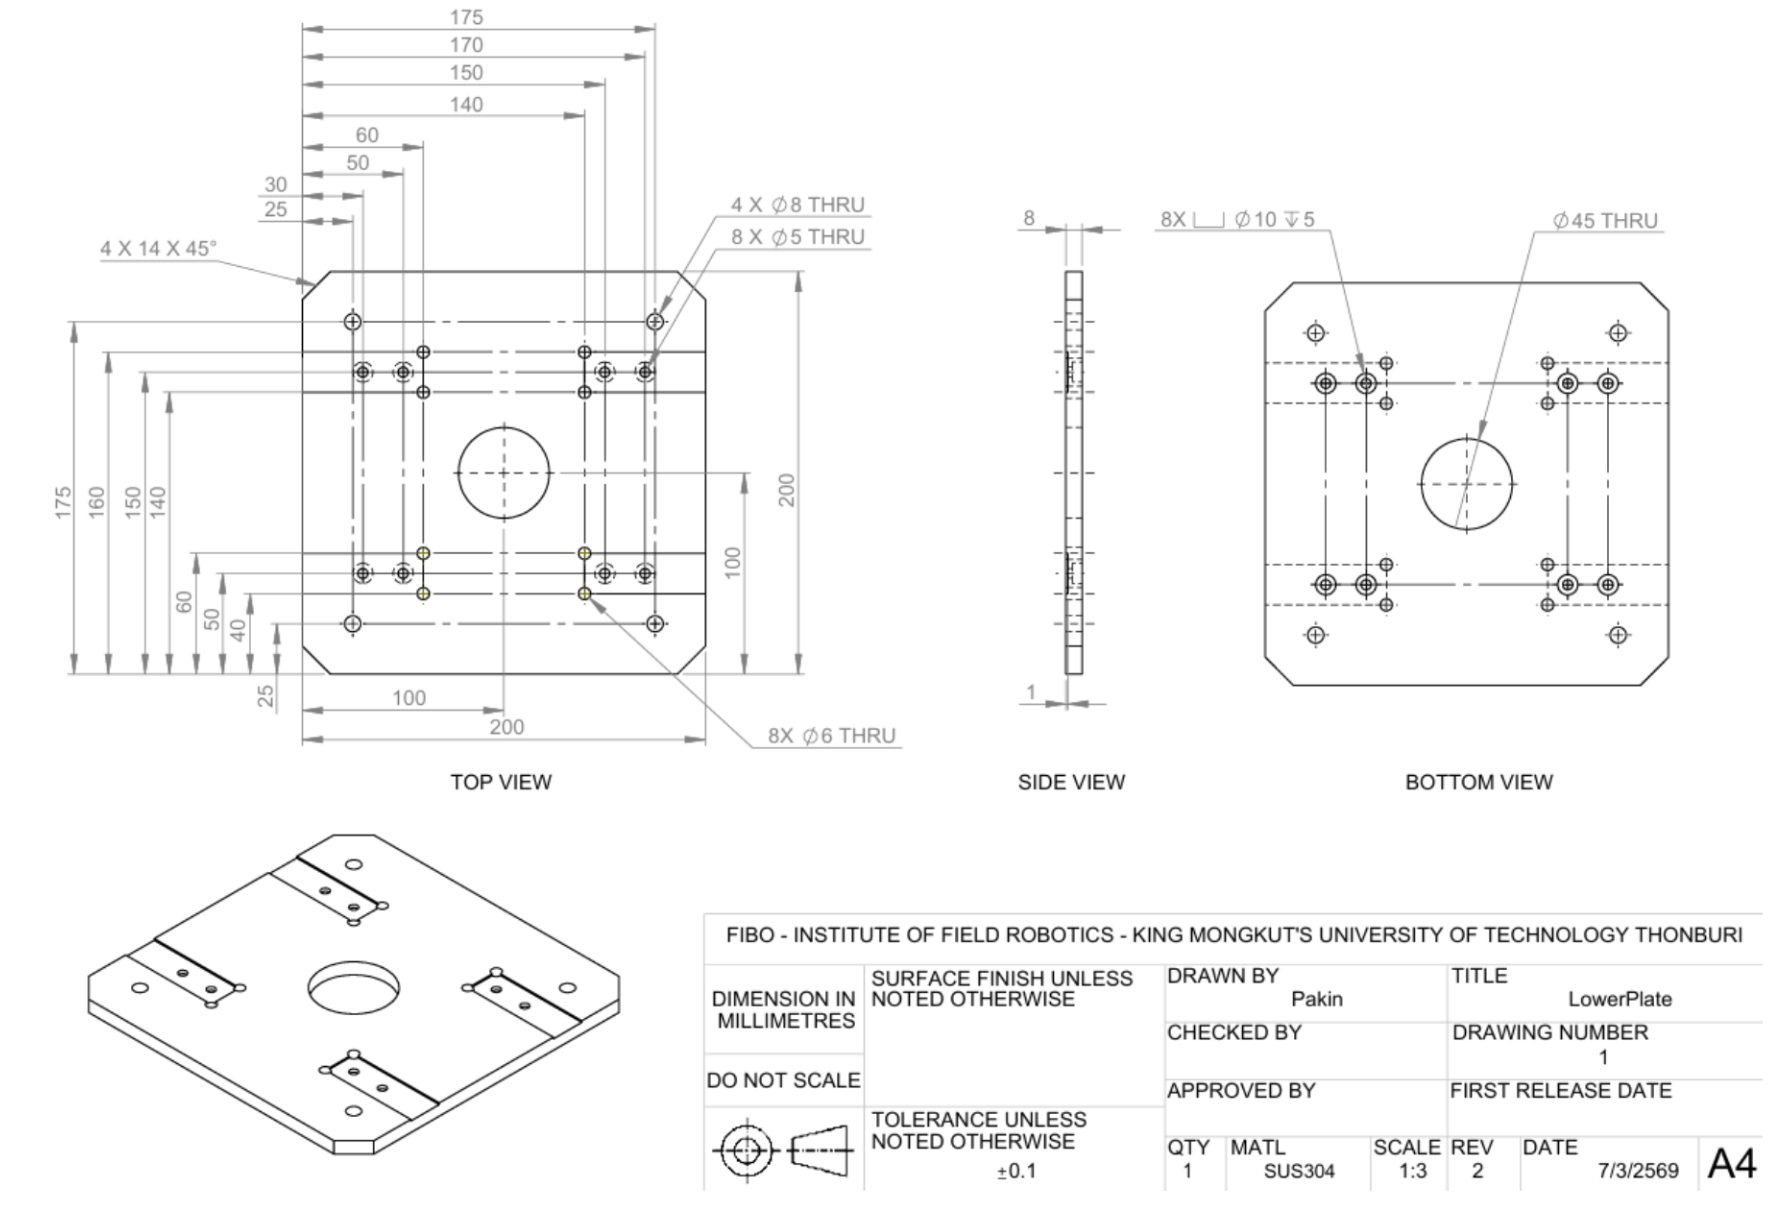
\includegraphics[width=\textwidth]{fig_drawing_lower_plate}
    \caption{Engineering Drawing: Lower Plate}
    \label{fig:drawing_lower_plate}
\end{figure}

\newpage

% ----------------------------------------------------------------------------

\begin{figure}[H]
    \centering
    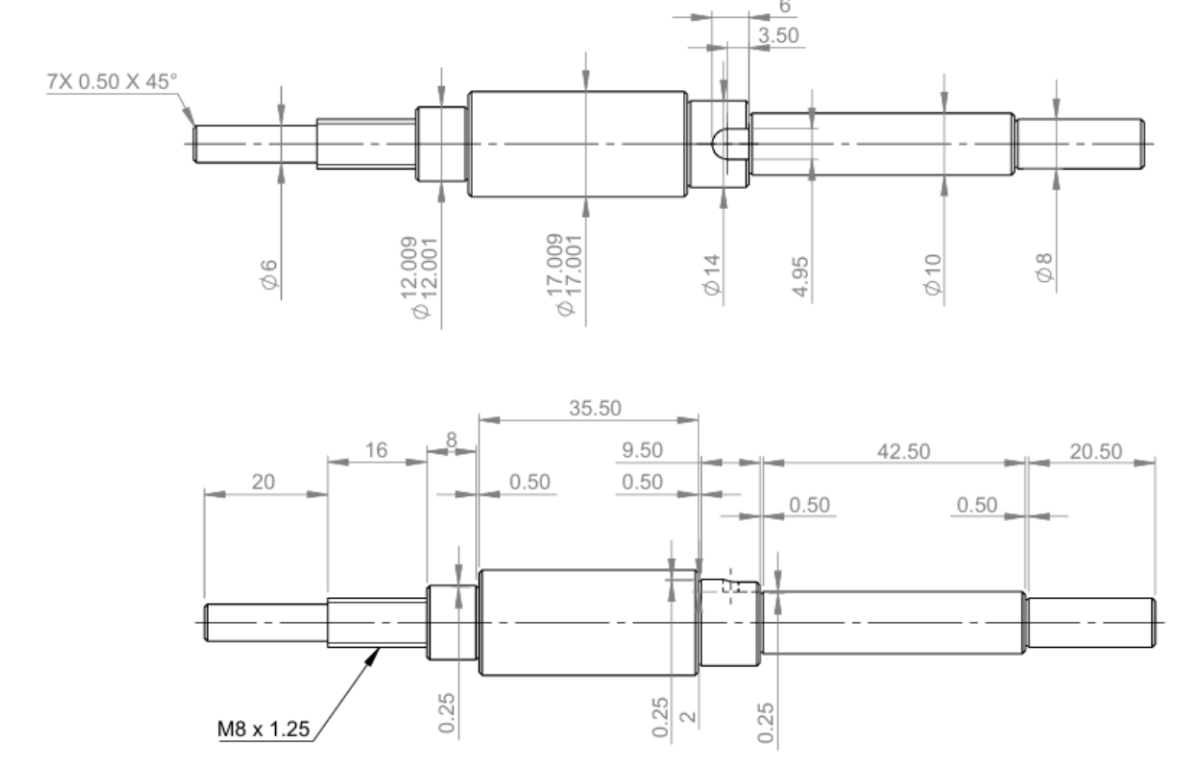
\includegraphics[width=\textwidth]{fig_drawing_step_shaft}
    \caption{Engineering Drawing: Step Shaft}
    \label{fig:drawing_step_shaft}
\end{figure}

\newpage

% ----------------------------------------------------------------------------

\begin{figure}[H]
    \centering
    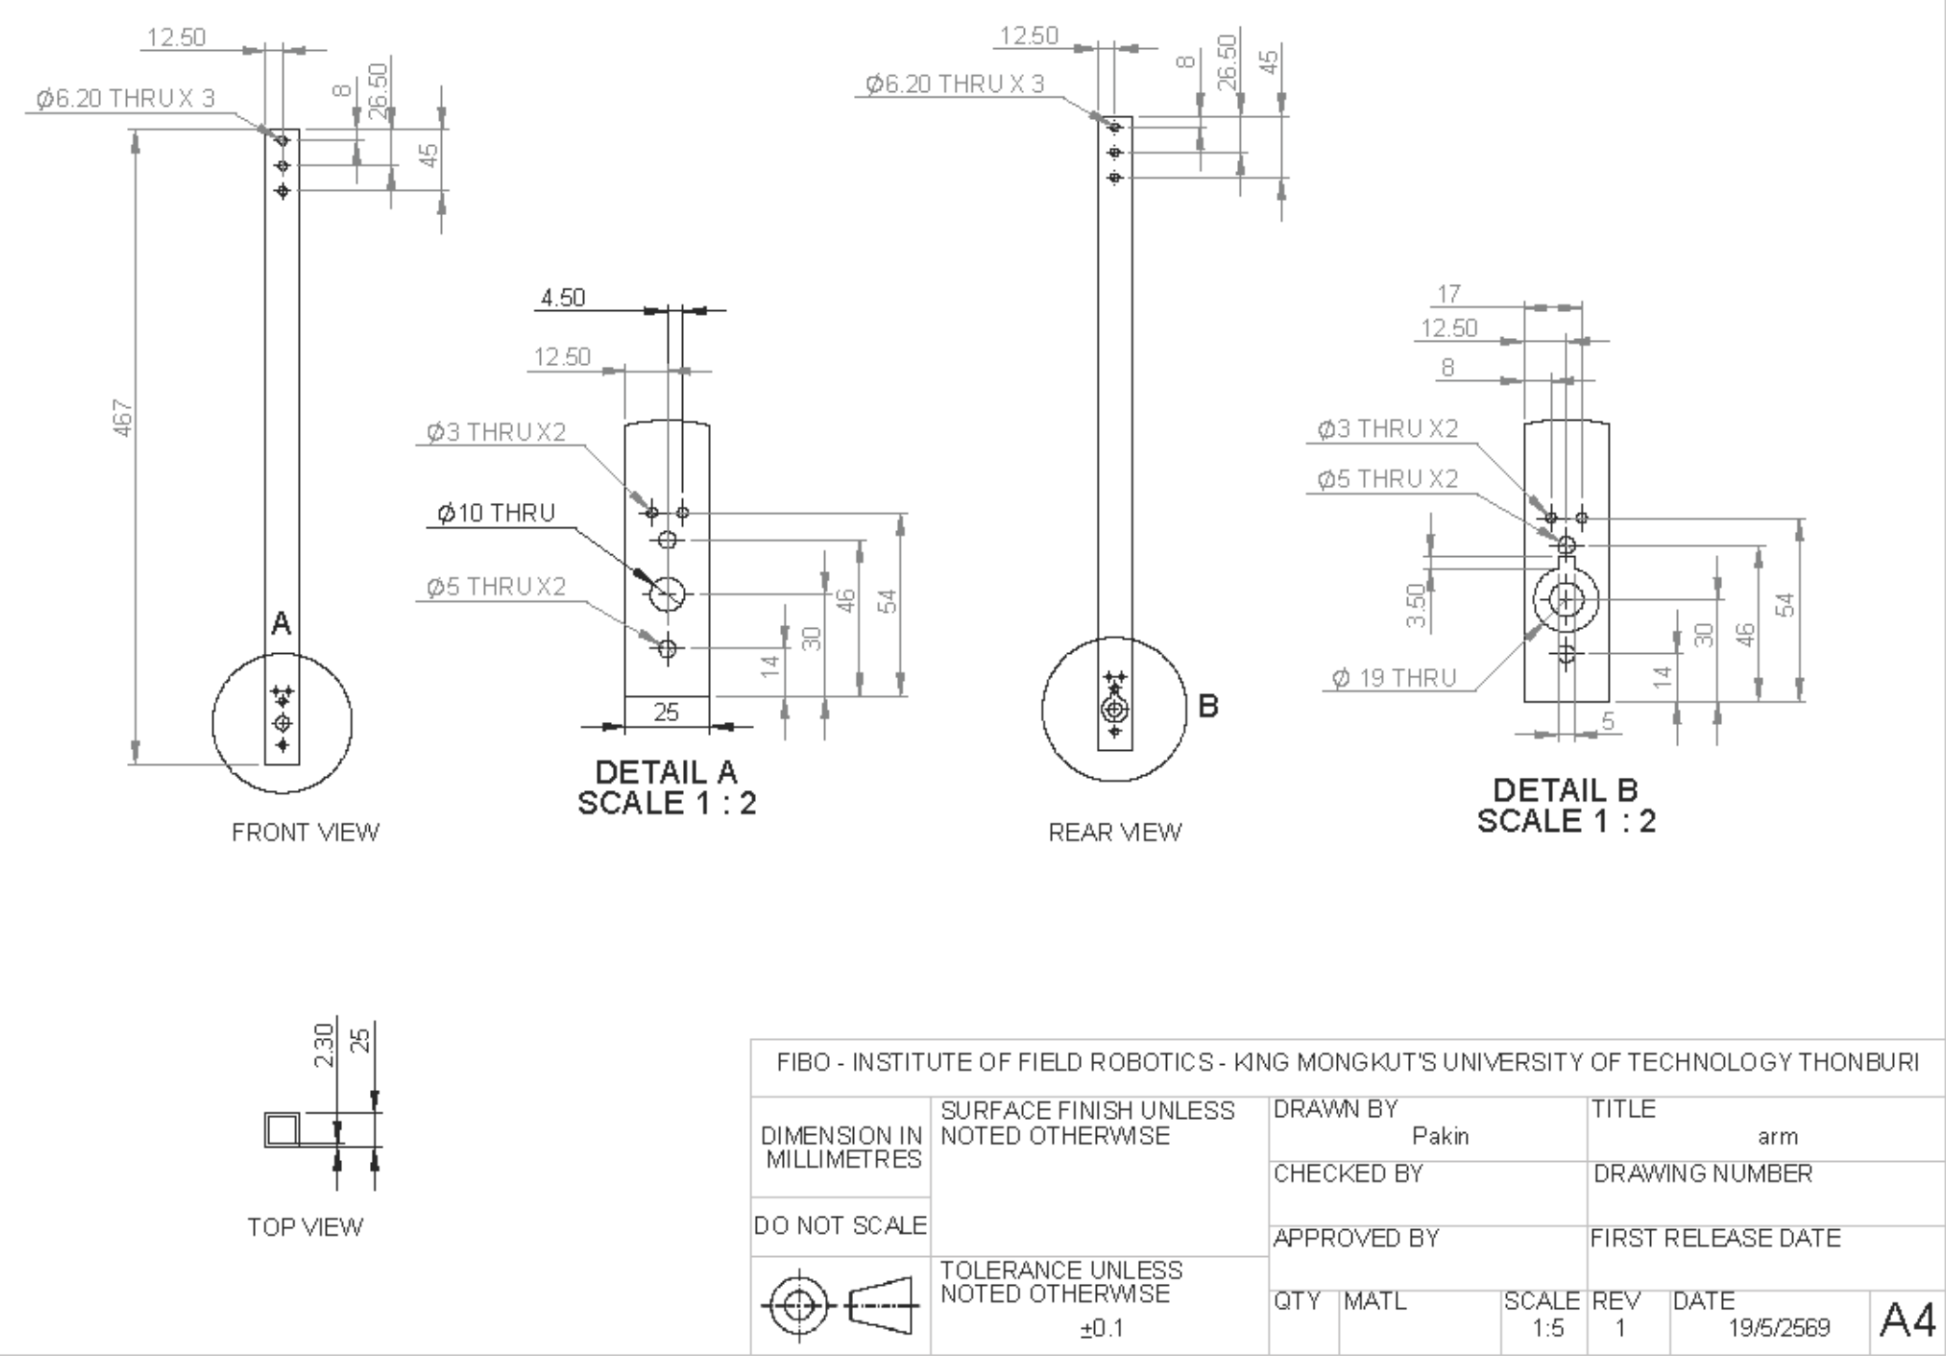
\includegraphics[width=\textwidth]{fig_drawing_arm}
    \caption{Engineering Drawing: Arm}
    \label{fig:drawing_arm}
\end{figure}

\newpage

% ----------------------------------------------------------------------------

\begin{figure}[H]
    \centering
    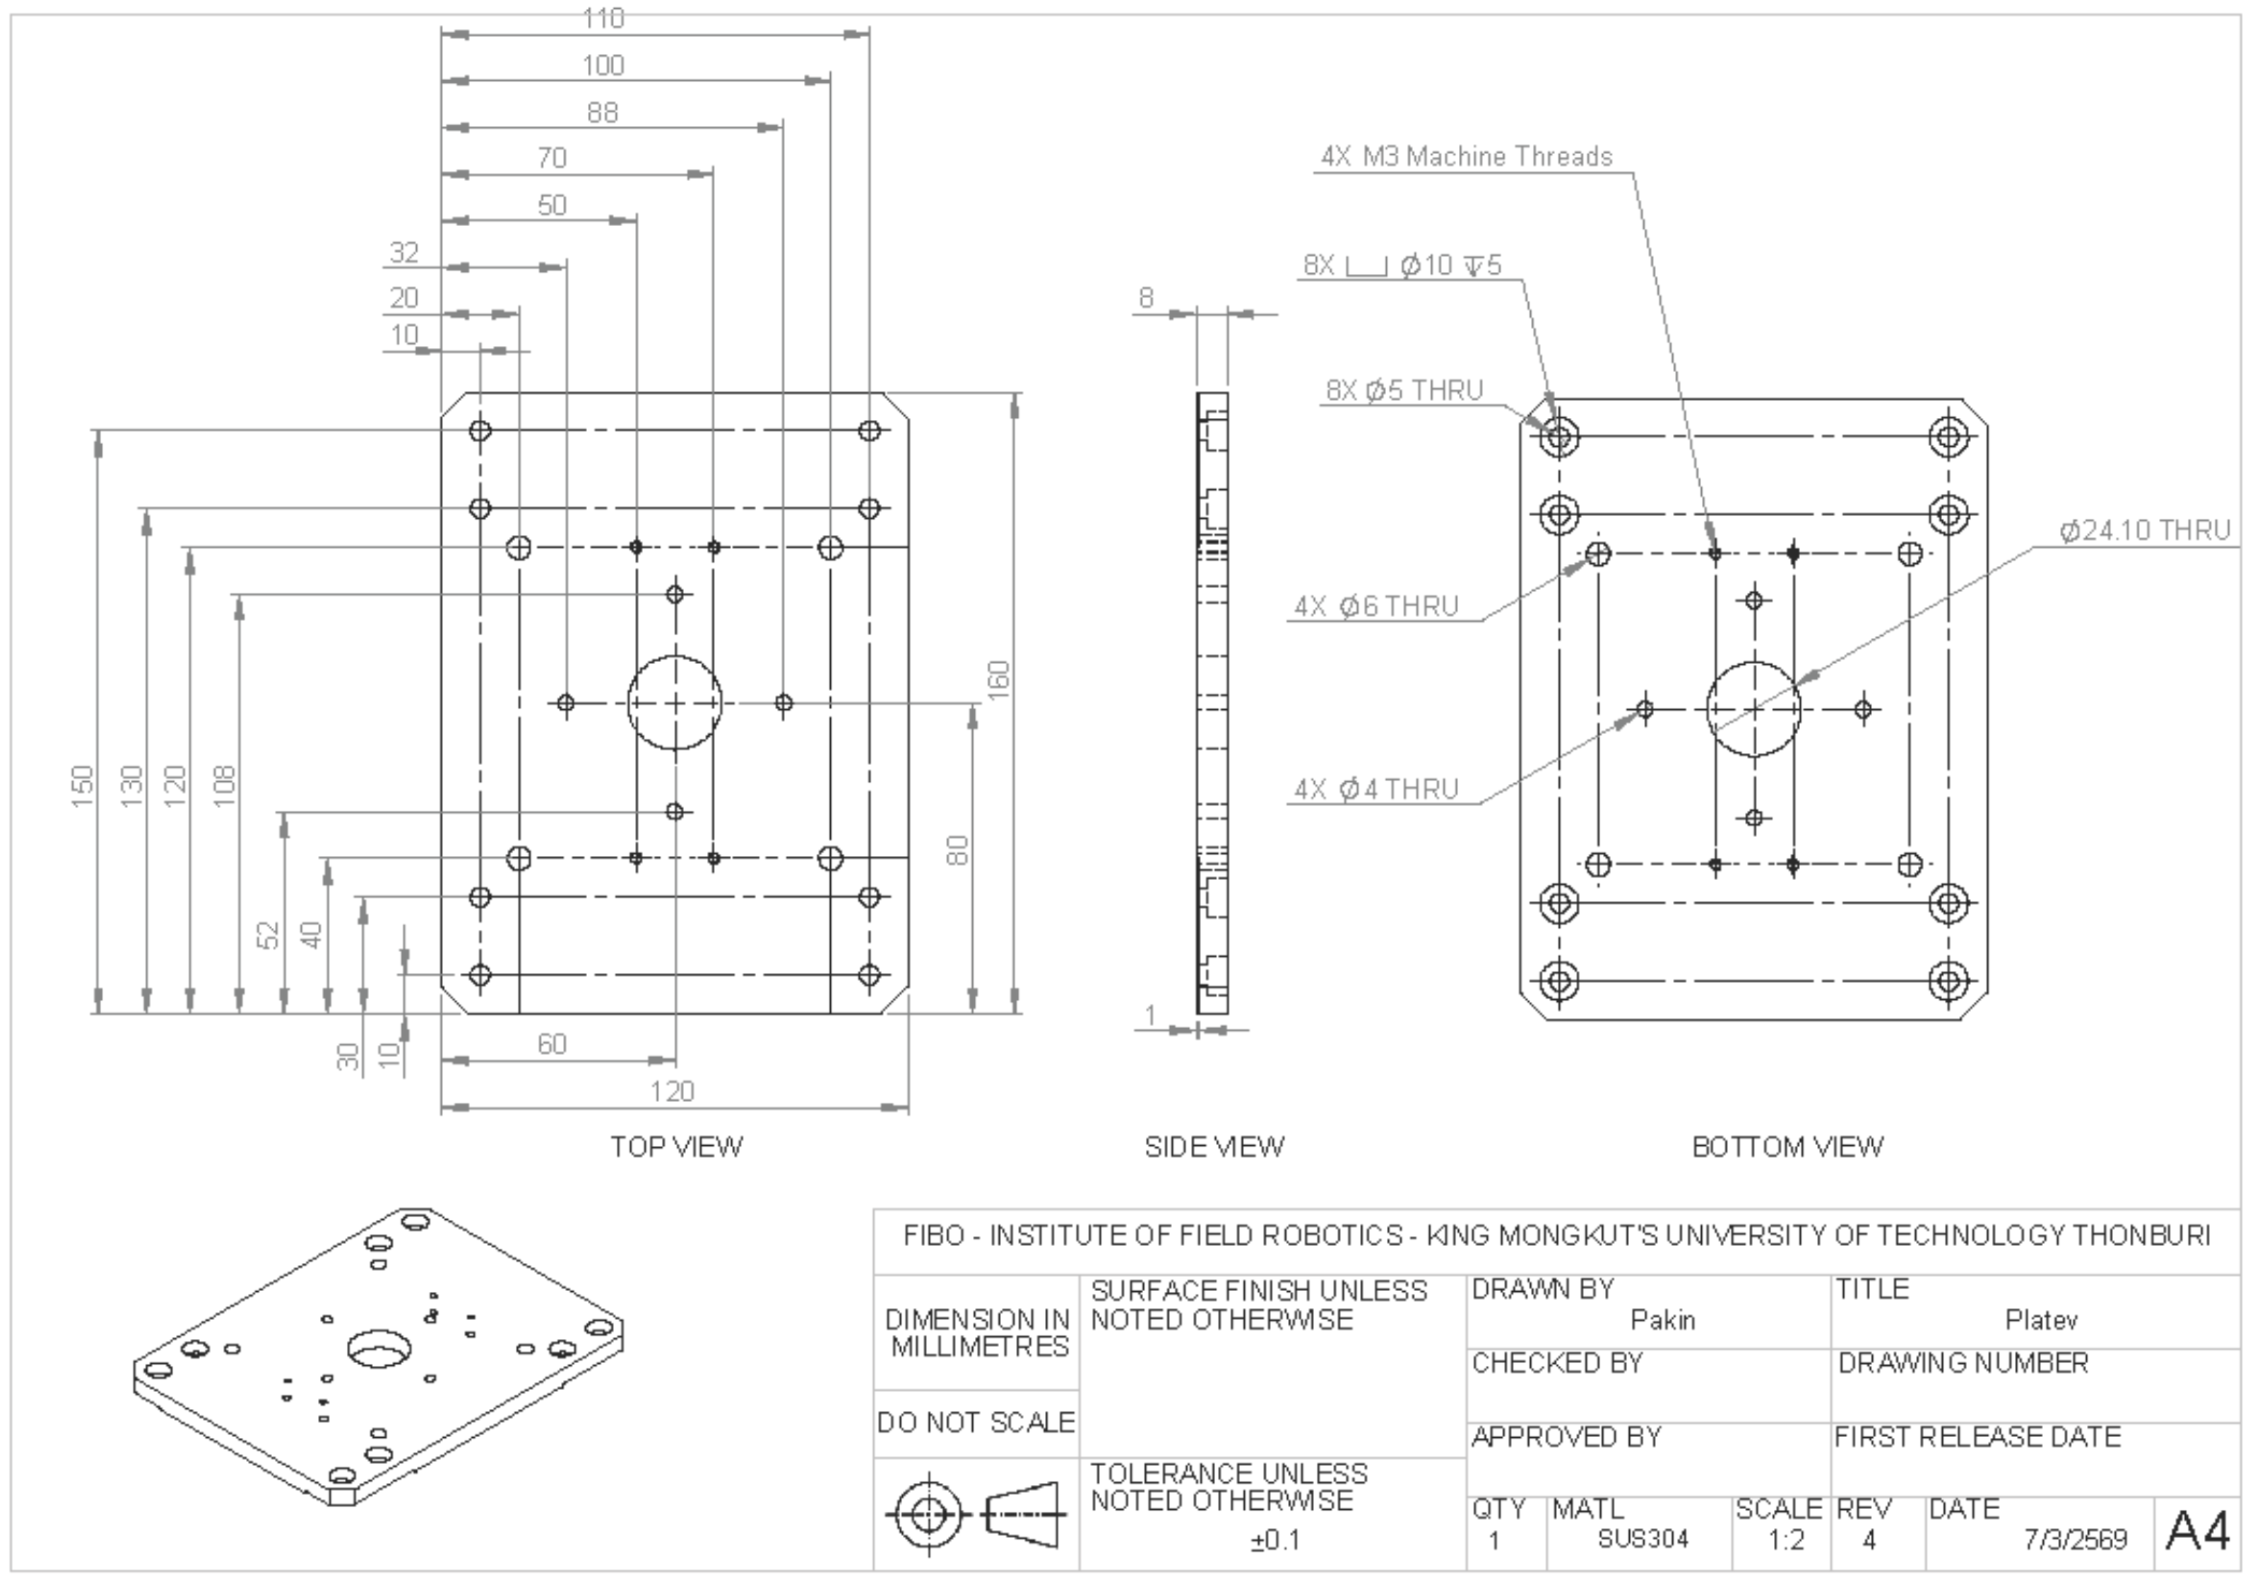
\includegraphics[width=\textwidth]{fig_drawing_plate_v}
    \caption{Engineering Drawing: Plate V}
    \label{fig:drawing_plate_v}
\end{figure}

% \input{sections/appendix_b_schematics.tex}
% \input{sections/appendix_c_code.tex}
% \input{sections/appendix_d_simscape.tex}

\end{document}